% Performance Before Outcomes -- version 9.0 (final): main text, Supplementary Information, references
% Build: pdflatex main; bibtex main; pdflatex main; pdflatex main
\documentclass[9pt,twocolumn,letterpaper]{extarticle}
\usepackage[T1]{fontenc}
\usepackage[utf8]{inputenc}
\usepackage{mathpazo}
\linespread{1.04}
\usepackage[scaled=0.90]{helvet}
\usepackage{amsmath,amssymb,amsthm,mathtools,bm}
\usepackage[letterpaper,left=0.62in,right=0.62in,top=0.80in,bottom=0.82in,columnsep=0.26in,headsep=0.22in,footskip=0.34in]{geometry}
\usepackage{microtype}
\usepackage{graphicx}
\usepackage[table]{xcolor}
\usepackage{booktabs,tabularx,array,multirow}
\usepackage{caption}
\usepackage{enumitem}
\usepackage{titlesec}
\usepackage{fancyhdr}
\usepackage{ragged2e}
\usepackage{stfloats}
\usepackage{flushend}
\usepackage[numbers,sort&compress]{natbib}
\usepackage[hyphens]{url}
\usepackage[colorlinks=true,linkcolor=accent,citecolor=accent,urlcolor=accent,pdftitle={Performance Before Outcomes},pdfauthor={Jepson Taylor and Erin Beilharz}]{hyperref}

\definecolor{ink}{HTML}{0B0B0B}
\definecolor{ink2}{HTML}{52514E}
\definecolor{accent}{HTML}{1C5CAB}
\definecolor{rulegray}{HTML}{C9C8C2}
\definecolor{band}{HTML}{F4F3EF}
\color{ink}

% ---- headings
\titleformat{\section}{\sffamily\bfseries\fontsize{11}{13}\selectfont}{\thesection}{0.6em}{}
\titleformat{\subsection}{\sffamily\bfseries\fontsize{9.4}{11.5}\selectfont}{\thesubsection}{0.5em}{}
\titleformat{\subsubsection}[runin]{\sffamily\bfseries\fontsize{9}{11}\selectfont}{}{0em}{}[.]
\titlespacing*{\section}{0pt}{11pt plus 2pt minus 2pt}{4.5pt}
\titlespacing*{\subsection}{0pt}{8pt plus 2pt minus 1pt}{3pt}
\titlespacing*{\subsubsection}{0pt}{5pt plus 1pt minus 1pt}{0.5em}
\setlength{\parindent}{1.1em}\setlength{\parskip}{0pt plus 0.9pt}
\raggedbottom % a column that cannot be filled ends short instead of opening a gap between paragraphs

% ---- floats and captions
\captionsetup{font={small},labelfont={bf,sf},labelsep=period,justification=justified,singlelinecheck=false,skip=5pt}
\captionsetup[table]{position=top,skip=4pt}
\renewcommand{\topfraction}{0.92}\renewcommand{\dbltopfraction}{0.92}\renewcommand{\bottomfraction}{0.6}
\renewcommand{\textfraction}{0.06}\renewcommand{\floatpagefraction}{0.75}\renewcommand{\dblfloatpagefraction}{0.7}
\setcounter{topnumber}{3}\setcounter{dbltopnumber}{3}\setcounter{totalnumber}{4}
\setlength{\textfloatsep}{10pt plus 2pt minus 2pt}\setlength{\dbltextfloatsep}{10pt plus 2pt minus 2pt}\setlength{\floatsep}{8pt plus 2pt minus 2pt}
\newcolumntype{L}{>{\RaggedRight\arraybackslash}X}
\newcolumntype{P}[1]{>{\RaggedRight\arraybackslash}p{#1}}
\newcolumntype{C}{>{\centering\arraybackslash}X}
\newcommand{\tablenote}[1]{\par\vspace{2pt}{\scriptsize\RaggedRight #1\par}}
\renewcommand{\arraystretch}{1.08}
\setlength{\tabcolsep}{4pt}

% ---- theorems
\newtheoremstyle{pbo}{5pt plus 1pt}{5pt plus 1pt}{\itshape}{}{\sffamily\bfseries\small}{.}{0.5em}{\thmname{#1}\thmnumber{ #2}\thmnote{ (#3)}}
\theoremstyle{pbo}
\newtheorem{proposition}{Proposition}
\newtheorem{corollary}{Corollary}
\newtheoremstyle{pbor}{5pt}{5pt}{}{}{\sffamily\bfseries\small}{.}{0.5em}{}
\theoremstyle{pbor}
\newtheorem*{remark}{Remark}

% ---- header and footer
\pagestyle{fancy}\fancyhf{}
\renewcommand{\headrulewidth}{0.3pt}\renewcommand{\headrule}{\color{rulegray}\hrule height 0.3pt}
\fancyhead[L]{\sffamily\scriptsize\color{ink2}PERFORMANCE BEFORE OUTCOMES}
\fancyhead[R]{\sffamily\scriptsize\color{ink2}Taylor and Beilharz \textperiodcentered{} preprint, November 2026}
\fancyfoot[C]{\sffamily\scriptsize\color{ink2}\thepage}

% ---- shorthands
\newcommand{\E}{\operatorname{E}}
\newcommand{\Var}{\operatorname{Var}}
\newcommand{\Cov}{\operatorname{Cov}}
\newcommand{\Corr}{\operatorname{Corr}}
\newcommand{\SD}{\operatorname{SD}}
\newcommand{\CV}{\operatorname{CV}}
\newcommand{\N}{\mathcal{N}}
\newcommand{\ccm}{\,cm$^3$}
\newcommand{\Hs}{\textit{H.~sapiens}}
\newcommand{\Homo}{\textit{Homo}}
\urlstyle{same}
\providecommand{\doi}[1]{doi:\,\href{https://doi.org/#1}{\nolinkurl{#1}}}
\setlist{leftmargin=1.3em,itemsep=1pt,topsep=3pt,parsep=0pt}
\frenchspacing
\emergencystretch=1.2em

\makeatletter\newcommand{\tabinput}[1]{\@@input #1 }\makeatother
% Generated by code/make_tex.py from results/*.json. Do not edit by hand.
\newcommand{\AimDomF}{0.070}
\newcommand{\AimDomG}{0.017}
\newcommand{\AimGain}{4.1}
\newcommand{\AimLoss}{2.6}
\newcommand{\AimMaxZ}{1.1}
\newcommand{\AimMixF}{0.053}
\newcommand{\AimMixG}{0.062}
\newcommand{\AimN}{12}
\newcommand{\AimPreF}{0.027}
\newcommand{\AimPreG}{0.072}
\newcommand{\AimRatDom}{0.25}
\newcommand{\AimRatPre}{2.7}
\newcommand{\AudAnc}{1\times10^{-16}}
\newcommand{\AudAsym}{5\times10^{-4}}
\newcommand{\AudBirths}{4\times10^{-16}}
\newcommand{\AudCK}{7\times10^{-4}}
\newcommand{\AudCeil}{0.004}
\newcommand{\AudCov}{6\times10^{-16}}
\newcommand{\AudCultures}{0}
\newcommand{\AudDelZ}{1.0}
\newcommand{\AudEnfCases}{355}
\newcommand{\AudEnfEq}{4\times10^{-16}}
\newcommand{\AudEnfZ}{1.0}
\newcommand{\AudEq}{1\times10^{-12}}
\newcommand{\AudFOC}{1\times10^{-7}}
\newcommand{\AudGss}{2\times10^{-16}}
\newcommand{\AudPoly}{1\times10^{-14}}
\newcommand{\AudQuad}{4\times10^{-17}}
\newcommand{\AudRoot}{2\times10^{-15}}
\newcommand{\AudSpeedGap}{0.007}
\newcommand{\AudSpeedLpm}{2\times10^{-13}}
\newcommand{\AudStage}{1\times10^{-15}}
\newcommand{\AudStageOpt}{1\times10^{-8}}
\newcommand{\AudWorldSign}{0}
\newcommand{\AudZ}{1.2}
\newcommand{\CcAgeM}{20.8}
\newcommand{\CcAgeN}{171}
\newcommand{\CcAgeW}{14.1}
\newcommand{\CcAloneM}{31}
\newcommand{\CcAloneMFor}{42}
\newcommand{\CcAloneW}{8}
\newcommand{\CcAloneWCount}{12}
\newcommand{\CcAloneWFor}{12}
\newcommand{\CcApprM}{21}
\newcommand{\CcApprW}{29}
\newcommand{\CcArrMenN}{148}
\newcommand{\CcArrWomenN}{151}
\newcommand{\CcBeat}{56}
\newcommand{\CcBeatN}{70}
\newcommand{\CcBeatPct}{80}
\newcommand{\CcBinN}{339}
\newcommand{\CcBrideService}{10}
\newcommand{\CcBridewealth}{57}
\newcommand{\CcCap}{58}
\newcommand{\CcCapN}{158}
\newcommand{\CcCapPct}{37}
\newcommand{\CcConsAsk}{39}
\newcommand{\CcConsMN}{54}
\newcommand{\CcConsMNec}{43}
\newcommand{\CcConsMNot}{17}
\newcommand{\CcConsN}{57}
\newcommand{\CcConsNec}{33}
\newcommand{\CcConsNot}{28}
\newcommand{\CcDivCommon}{49}
\newcommand{\CcDivCommonPct}{58}
\newcommand{\CcDivEq}{72}
\newcommand{\CcDivEqPct}{77}
\newcommand{\CcDivFreqN}{85}
\newcommand{\CcDivMaleOnly}{5}
\newcommand{\CcDivN}{93}
\newcommand{\CcDivRare}{25}
\newcommand{\CcDowry}{3}
\newcommand{\CcEaN}{1{,}291}
\newcommand{\CcEitherM}{18}
\newcommand{\CcEitherW}{18}
\newcommand{\CcForArrN}{41}
\newcommand{\CcForN}{46}
\newcommand{\CcForService}{16}
\newcommand{\CcGamesAny}{460}
\newcommand{\CcGamesAnyPct}{95}
\newcommand{\CcGamesForAny}{233}
\newcommand{\CcGamesForN}{237}
\newcommand{\CcGamesN}{486}
\newcommand{\CcGap}{6.7}
\newcommand{\CcGapCI}{5.9 to 7.4}
\newcommand{\CcGapHigh}{8.6}
\newcommand{\CcGapLow}{4.7}
\newcommand{\CcGapPolyCI}{0.41 to 0.74}
\newcommand{\CcGapPolyR}{0.60}
\newcommand{\CcMenOlderPct}{98}
\newcommand{\CcMono}{16}
\newcommand{\CcMonoN}{1{,}257}
\newcommand{\CcNoObjM}{19}
\newcommand{\CcNoObjW}{33}
\newcommand{\CcNoObjWPct}{22}
\newcommand{\CcPairDau}{44}
\newcommand{\CcPairN}{142}
\newcommand{\CcPairSame}{96}
\newcommand{\CcPairSon}{2}
\newcommand{\CcParM}{30}
\newcommand{\CcParMFor}{30}
\newcommand{\CcParW}{45}
\newcommand{\CcParWFor}{54}
\newcommand{\CcPolyMed}{10}
\newcommand{\CcPolyN}{128}
\newcommand{\CcPolyWomenMed}{10}
\newcommand{\CcPolyWomenN}{145}
\newcommand{\CcProdService}{8}
\newcommand{\CcRapeAbs}{8}
\newcommand{\CcRapeCom}{13}
\newcommand{\CcRapeComPct}{42}
\newcommand{\CcRapeN}{31}
\newcommand{\CcRapeOwnCom}{2}
\newcommand{\CcRapeOwnN}{12}
\newcommand{\CcRapeParCom}{8}
\newcommand{\CcRapeParN}{11}
\newcommand{\CcRapeRare}{10}
\newcommand{\CcRelMenOlder}{61}
\newcommand{\CcRelN}{70}
\newcommand{\CcRelWomenOlder}{2}
\newcommand{\CcSanAbs}{45}
\newcommand{\CcSanForN}{29}
\newcommand{\CcSanForPres}{13}
\newcommand{\CcSanN}{95}
\newcommand{\CcSanPres}{50}
\newcommand{\CcSanPresPct}{53}
\newcommand{\CcSccsN}{186}
\newcommand{\CcTrN}{1{,}272}
\newcommand{\CcWarGreat}{61}
\newcommand{\CcWarGreatPct}{40}
\newcommand{\CcWarN}{151}
\newcommand{\CueSG}{3.7\times10^{-5}}
\newcommand{\CueSGse}{6.3\times10^{-5}}
\newcommand{\CueSQ}{0.020}
\newcommand{\DAdiff}{9.9\times10^{-4}}
\newcommand{\DAmOne}{0.37}
\newcommand{\DAmTwo}{0.18}
\newcommand{\DAmZero}{0.50}
\newcommand{\DesILin}{5.5}
\newcommand{\DesISq}{2.1}
\newcommand{\DesIdespot}{19}
\newcommand{\DesIntHi}{3.0}
\newcommand{\DesIntLo}{1.9}
\newcommand{\DesKLin}{9.5}
\newcommand{\DesKSq}{13}
\newcommand{\DesShareLin}{0.53}
\newcommand{\DesShareSq}{0.35}
\newcommand{\DesThrLin}{0.05}
\newcommand{\DesThrSq}{0.16}
\newcommand{\ENineMaxZ}{1.2}
\newcommand{\ENineN}{20}
\newcommand{\EOneExact}{0.075556}
\newcommand{\EOneMC}{0.075637}
\newcommand{\EOneMaxDiff}{2.7\times10^{-4}}
\newcommand{\EThreeMaxZ}{2.7}
\newcommand{\EThreeN}{38}
\newcommand{\ETwoMaxZ}{2.6}
\newcommand{\ETwoN}{21}
\newcommand{\EnfCapFifth}{0.32}
\newcommand{\EnfCapHalf}{0.59}
\newcommand{\EnfCrowdAt}{0.58}
\newcommand{\EnfCrowdMin}{0.79}
\newcommand{\EnfCrowdT}{1.5}
\newcommand{\EnfEstar}{0.39}
\newcommand{\EnfIbmDiff}{0.006}
\newcommand{\EnfPmax}{0.18}
\newcommand{\EnfRecErr}{1\times10^{-14}}
\newcommand{\EnfT}{0.6}
\newcommand{\FixHi}{0.0801}
\newcommand{\FixLo}{0.0566}
\newcommand{\FixRatio}{1.42}
\newcommand{\FosAICLin}{43}
\newcommand{\FosAICOne}{21}
\newcommand{\FosAICPub}{6.9}
\newcommand{\FosAICStep}{4.8}
\newcommand{\FosBICFree}{9.7}
\newcommand{\FosBICLin}{33}
\newcommand{\FosBICStep}{7.9}
\newcommand{\FosBins}{26}
\newcommand{\FosBoot}{400}
\newcommand{\FosBpA}{2.15}
\newcommand{\FosBpB}{1.45}
\newcommand{\FosBpC}{0.65}
\newcommand{\FosCIA}{2.0--2.8}
\newcommand{\FosCIB}{0.7--1.7}
\newcommand{\FosCIC}{0.4--1.1}
\newcommand{\FosFreeBpA}{2.0}
\newcommand{\FosFreeBpB}{1.7}
\newcommand{\FosFreeBpC}{0.45}
\newcommand{\FosFreeSlA}{0.08}
\newcommand{\FosFreeSlB}{1.61}
\newcommand{\FosFreeSlC}{0.24}
\newcommand{\FosFreeSlD}{0.82}
\newcommand{\FosLevEnd}{1{,}477}
\newcommand{\FosLevI}{443}
\newcommand{\FosLevIII}{908}
\newcommand{\FosN}{233}
\newcommand{\FosRateHi}{1.1}
\newcommand{\FosRateII}{2.6}
\newcommand{\FosRateIV}{1.9}
\newcommand{\FosRateLo}{0.8}
\newcommand{\FosSDw}{0.116}
\newcommand{\FosSlII}{1.03}
\newcommand{\FosSlIV}{0.76}
\newcommand{\FosSlopeBin}{0.387}
\newcommand{\FosSlopeBinSE}{0.029}
\newcommand{\FosSlopeSpec}{0.434}
\newcommand{\FosSlopeSpecSE}{0.010}
\newcommand{\FosSpan}{3.19}
\newcommand{\FosStI}{0.12}
\newcommand{\FosStIII}{0.10}
\newcommand{\FosStIIIN}{19}
\newcommand{\FosStIIISE}{0.21}
\newcommand{\FosStIN}{16}
\newcommand{\FosStISE}{0.10}
\newcommand{\GssAfbRM}{0.30}
\newcommand{\GssAfbRW}{0.40}
\newcommand{\GssBatMGrad}{\ensuremath{-0.030}}
\newcommand{\GssBatMGradCI}{\ensuremath{-0.044} to \ensuremath{-0.014}}
\newcommand{\GssBatMMed}{5}
\newcommand{\GssBatMOne}{2.69}
\newcommand{\GssBatMTwenty}{2.23}
\newcommand{\GssBatWGrad}{\ensuremath{-0.059}}
\newcommand{\GssBatWGradCI}{\ensuremath{-0.069} to \ensuremath{-0.050}}
\newcommand{\GssBatWMed}{2}
\newcommand{\GssBatWOne}{2.76}
\newcommand{\GssBatWTwenty}{1.73}
\newcommand{\GssBoot}{2{,}000}
\newcommand{\GssCheck}{5\times10^{-16}}
\newcommand{\GssChlMIncHi}{11.5}
\newcommand{\GssChlMIncLo}{20.5}
\newcommand{\GssChlWIncHi}{17.6}
\newcommand{\GssChlWIncLo}{8.9}
\newcommand{\GssConvMNew}{\ensuremath{-0.011}}
\newcommand{\GssConvMNewCI}{\ensuremath{-0.041} to \ensuremath{+0.017}}
\newcommand{\GssConvMOld}{\ensuremath{+0.015}}
\newcommand{\GssConvWNew}{\ensuremath{-0.064}}
\newcommand{\GssConvWNewCI}{\ensuremath{-0.088} to \ensuremath{-0.039}}
\newcommand{\GssConvWOld}{\ensuremath{-0.023}}
\newcommand{\GssDivChlM}{17.2}
\newcommand{\GssDivChlW}{10.1}
\newcommand{\GssDivDiff}{\ensuremath{-0.07}}
\newcommand{\GssDivDiffCI}{\ensuremath{-0.12} to \ensuremath{-0.02}}
\newcommand{\GssDivM}{\ensuremath{-0.07}}
\newcommand{\GssDivMCI}{\ensuremath{-0.11} to \ensuremath{-0.03}}
\newcommand{\GssDivW}{0.00}
\newcommand{\GssDivWCI}{\ensuremath{-0.03} to \ensuremath{+0.03}}
\newcommand{\GssFloorM}{8.0}
\newcommand{\GssFloorMCI}{3.4 to 12.7}
\newcommand{\GssGateMFirst}{1}
\newcommand{\GssGateMFirstCI}{0 to 3}
\newcommand{\GssGateMNew}{31}
\newcommand{\GssGateMNewCI}{26 to 37}
\newcommand{\GssGateMOld}{9}
\newcommand{\GssGateMOldCI}{5 to 13}
\newcommand{\GssGateWFirst}{7}
\newcommand{\GssGateWFirstCI}{1 to 15}
\newcommand{\GssGateWNew}{61}
\newcommand{\GssGateWNewCI}{56 to 66}
\newcommand{\GssGateWOld}{18}
\newcommand{\GssGateWOldCI}{12 to 24}
\newcommand{\GssHomNew}{0.59}
\newcommand{\GssHomOld}{0.62}
\newcommand{\GssHypDiffYoung}{13}
\newcommand{\GssHypDiffYoungCI}{9 to 18}
\newcommand{\GssHypLessMid}{39}
\newcommand{\GssHypLessNew}{32}
\newcommand{\GssHypLessOld}{38}
\newcommand{\GssHypLessYoung}{27}
\newcommand{\GssHypMoreMid}{30}
\newcommand{\GssHypMoreNew}{36}
\newcommand{\GssHypMoreOld}{32}
\newcommand{\GssHypMoreYoung}{40}
\newcommand{\GssHypR}{0.61}
\newcommand{\GssIM}{0.53}
\newcommand{\GssIW}{0.49}
\newcommand{\GssInMFirst}{100.0}
\newcommand{\GssInMNew}{94.9}
\newcommand{\GssInMOld}{99.6}
\newcommand{\GssInWFirst}{99.8}
\newcommand{\GssInWNew}{91.7}
\newcommand{\GssInWOld}{99.4}
\newcommand{\GssIncDiffAcc}{\ensuremath{+0.085}}
\newcommand{\GssIncDiffAccCI}{\ensuremath{+0.070} to \ensuremath{+0.099}}
\newcommand{\GssIncMAcc}{\ensuremath{+0.047}}
\newcommand{\GssIncMAccCI}{\ensuremath{+0.036} to \ensuremath{+0.059}}
\newcommand{\GssIncMConv}{\ensuremath{+0.001}}
\newcommand{\GssIncMConvCI}{\ensuremath{-0.009} to \ensuremath{+0.013}}
\newcommand{\GssIncMNum}{\ensuremath{-0.034}}
\newcommand{\GssIncMNumCI}{\ensuremath{-0.050} to \ensuremath{-0.017}}
\newcommand{\GssIncMPair}{\ensuremath{+0.046}}
\newcommand{\GssIncMPairCI}{\ensuremath{+0.037} to \ensuremath{+0.054}}
\newcommand{\GssIncMTot}{\ensuremath{+0.013}}
\newcommand{\GssIncMTotCI}{\ensuremath{-0.008} to \ensuremath{+0.034}}
\newcommand{\GssIncWAcc}{\ensuremath{-0.038}}
\newcommand{\GssIncWAccCI}{\ensuremath{-0.047} to \ensuremath{-0.028}}
\newcommand{\GssIncWConv}{\ensuremath{-0.038}}
\newcommand{\GssIncWConvCI}{\ensuremath{-0.049} to \ensuremath{-0.028}}
\newcommand{\GssIncWNum}{\ensuremath{-0.078}}
\newcommand{\GssIncWNumCI}{\ensuremath{-0.094} to \ensuremath{-0.063}}
\newcommand{\GssIncWPair}{\ensuremath{+0.001}}
\newcommand{\GssIncWPairCI}{\ensuremath{-0.007} to \ensuremath{+0.009}}
\newcommand{\GssIncWTot}{\ensuremath{-0.116}}
\newcommand{\GssIncWTotCI}{\ensuremath{-0.134} to \ensuremath{-0.098}}
\newcommand{\GssIntChlM}{8.6}
\newcommand{\GssIntChlW}{8.4}
\newcommand{\GssN}{34{,}092}
\newcommand{\GssNevMNew}{13.3}
\newcommand{\GssNevMOld}{4.5}
\newcommand{\GssNevWNew}{11.4}
\newcommand{\GssNevWOld}{2.9}
\newcommand{\GssNmMFive}{2.6}
\newcommand{\GssNmMOne}{15.5}
\newcommand{\GssOutMFirst}{0.0}
\newcommand{\GssOutMFirstCI}{0.0 to 0.1}
\newcommand{\GssOutMNew}{5.1}
\newcommand{\GssOutMNewCI}{3.6 to 6.7}
\newcommand{\GssOutMOld}{0.4}
\newcommand{\GssOutMOldCI}{0.2 to 0.6}
\newcommand{\GssOutWFirst}{0.2}
\newcommand{\GssOutWFirstCI}{0.0 to 0.6}
\newcommand{\GssOutWNew}{8.3}
\newcommand{\GssOutWNewCI}{6.8 to 9.8}
\newcommand{\GssOutWOld}{0.6}
\newcommand{\GssOutWOldCI}{0.4 to 0.9}
\newcommand{\GssPairMChange}{\ensuremath{+0.052}}
\newcommand{\GssPairMChangeCI}{\ensuremath{+0.027} to \ensuremath{+0.077}}
\newcommand{\GssPairMNew}{\ensuremath{+0.078}}
\newcommand{\GssPairMNewCI}{\ensuremath{+0.056} to \ensuremath{+0.102}}
\newcommand{\GssPairMOld}{\ensuremath{+0.027}}
\newcommand{\GssPairMOldCI}{\ensuremath{+0.016} to \ensuremath{+0.039}}
\newcommand{\GssPairWChange}{\ensuremath{+0.029}}
\newcommand{\GssPairWChangeCI}{\ensuremath{+0.010} to \ensuremath{+0.050}}
\newcommand{\GssPairWNew}{\ensuremath{+0.020}}
\newcommand{\GssPairWNewCI}{\ensuremath{+0.003} to \ensuremath{+0.038}}
\newcommand{\GssPairWOld}{\ensuremath{-0.009}}
\newcommand{\GssPairWOldCI}{\ensuremath{-0.018} to 0.000}
\newcommand{\GssPartIncM}{\ensuremath{+0.01}}
\newcommand{\GssPartIncMCI}{\ensuremath{-0.03} to \ensuremath{+0.04}}
\newcommand{\GssPartIncW}{\ensuremath{+0.09}}
\newcommand{\GssPartIncWCI}{\ensuremath{+0.06} to \ensuremath{+0.12}}
\newcommand{\GssPartMedM}{5}
\newcommand{\GssPartMedW}{2}
\newcommand{\GssPartPreM}{\ensuremath{-0.01}}
\newcommand{\GssPartPreMCI}{\ensuremath{-0.04} to \ensuremath{+0.01}}
\newcommand{\GssPartPreW}{\ensuremath{+0.02}}
\newcommand{\GssPartPreWCI}{\ensuremath{-0.01} to \ensuremath{+0.04}}
\newcommand{\GssPartSchM}{\ensuremath{-0.01}}
\newcommand{\GssPartSchMCI}{\ensuremath{-0.04} to \ensuremath{+0.01}}
\newcommand{\GssPartSchW}{\ensuremath{+0.04}}
\newcommand{\GssPartSchWCI}{\ensuremath{+0.02} to \ensuremath{+0.07}}
\newcommand{\GssPartVocM}{\ensuremath{+0.05}}
\newcommand{\GssPartVocMCI}{\ensuremath{+0.01} to \ensuremath{+0.08}}
\newcommand{\GssPartVocW}{\ensuremath{+0.09}}
\newcommand{\GssPartVocWCI}{\ensuremath{+0.07} to \ensuremath{+0.13}}
\newcommand{\GssPlHighM}{10.2}
\newcommand{\GssPlHighW}{7.7}
\newcommand{\GssPlLowM}{17.6}
\newcommand{\GssPlLowW}{10.9}
\newcommand{\GssPlMHi}{10.2}
\newcommand{\GssPlMLo}{17.6}
\newcommand{\GssPlMNew}{15.5}
\newcommand{\GssPlMNone}{22.9}
\newcommand{\GssPlMOld}{8.7}
\newcommand{\GssPlWNew}{11.1}
\newcommand{\GssPlWOld}{7.1}
\newcommand{\GssPreDiffAcc}{\ensuremath{+0.035}}
\newcommand{\GssPreDiffAccCI}{\ensuremath{+0.026} to \ensuremath{+0.045}}
\newcommand{\GssPreMAcc}{\ensuremath{+0.016}}
\newcommand{\GssPreMAccCI}{\ensuremath{+0.008} to \ensuremath{+0.024}}
\newcommand{\GssPreMConv}{\ensuremath{-0.007}}
\newcommand{\GssPreMConvCI}{\ensuremath{-0.014} to \ensuremath{+0.001}}
\newcommand{\GssPreMNum}{\ensuremath{-0.046}}
\newcommand{\GssPreMNumCI}{\ensuremath{-0.057} to \ensuremath{-0.036}}
\newcommand{\GssPreMPair}{\ensuremath{+0.023}}
\newcommand{\GssPreMPairCI}{\ensuremath{+0.018} to \ensuremath{+0.028}}
\newcommand{\GssPreMTot}{\ensuremath{-0.031}}
\newcommand{\GssPreMTotCI}{\ensuremath{-0.044} to \ensuremath{-0.017}}
\newcommand{\GssPreWAcc}{\ensuremath{-0.019}}
\newcommand{\GssPreWAccCI}{\ensuremath{-0.026} to \ensuremath{-0.013}}
\newcommand{\GssPreWConv}{\ensuremath{-0.020}}
\newcommand{\GssPreWConvCI}{\ensuremath{-0.027} to \ensuremath{-0.014}}
\newcommand{\GssPreWNum}{\ensuremath{-0.061}}
\newcommand{\GssPreWNumCI}{\ensuremath{-0.071} to \ensuremath{-0.051}}
\newcommand{\GssPreWPair}{\ensuremath{+0.001}}
\newcommand{\GssPreWPairCI}{\ensuremath{-0.003} to \ensuremath{+0.005}}
\newcommand{\GssPreWTot}{\ensuremath{-0.081}}
\newcommand{\GssPreWTotCI}{\ensuremath{-0.093} to \ensuremath{-0.069}}
\newcommand{\GssQfMFive}{10.5}
\newcommand{\GssQfMOne}{21.9}
\newcommand{\GssQfMThree}{12.2}
\newcommand{\GssQfMTwo}{17.2}
\newcommand{\GssQfWFive}{19.5}
\newcommand{\GssQfWOne}{9.5}
\newcommand{\GssRemDiff}{\ensuremath{+0.08}}
\newcommand{\GssRemDiffCI}{\ensuremath{+0.03} to \ensuremath{+0.13}}
\newcommand{\GssRemM}{\ensuremath{+0.07}}
\newcommand{\GssRemMCI}{\ensuremath{+0.03} to \ensuremath{+0.10}}
\newcommand{\GssRemW}{\ensuremath{-0.02}}
\newcommand{\GssRemWCI}{\ensuremath{-0.05} to \ensuremath{+0.02}}
\newcommand{\GssSchDiffAcc}{\ensuremath{+0.035}}
\newcommand{\GssSchDiffAccCI}{\ensuremath{+0.025} to \ensuremath{+0.045}}
\newcommand{\GssSchMAcc}{\ensuremath{-0.003}}
\newcommand{\GssSchMAccCI}{\ensuremath{-0.012} to \ensuremath{+0.005}}
\newcommand{\GssSchMConv}{\ensuremath{-0.018}}
\newcommand{\GssSchMConvCI}{\ensuremath{-0.026} to \ensuremath{-0.010}}
\newcommand{\GssSchMNum}{\ensuremath{-0.081}}
\newcommand{\GssSchMNumCI}{\ensuremath{-0.094} to \ensuremath{-0.068}}
\newcommand{\GssSchMPair}{\ensuremath{+0.015}}
\newcommand{\GssSchMPairCI}{\ensuremath{+0.009} to \ensuremath{+0.021}}
\newcommand{\GssSchMTot}{\ensuremath{-0.085}}
\newcommand{\GssSchMTotCI}{\ensuremath{-0.100} to \ensuremath{-0.069}}
\newcommand{\GssSchWAcc}{\ensuremath{-0.038}}
\newcommand{\GssSchWAccCI}{\ensuremath{-0.044} to \ensuremath{-0.032}}
\newcommand{\GssSchWConv}{\ensuremath{-0.034}}
\newcommand{\GssSchWConvCI}{\ensuremath{-0.041} to \ensuremath{-0.028}}
\newcommand{\GssSchWNum}{\ensuremath{-0.126}}
\newcommand{\GssSchWNumCI}{\ensuremath{-0.137} to \ensuremath{-0.115}}
\newcommand{\GssSchWPair}{\ensuremath{-0.004}}
\newcommand{\GssSchWPairCI}{\ensuremath{-0.009} to \ensuremath{+0.001}}
\newcommand{\GssSchWTot}{\ensuremath{-0.164}}
\newcommand{\GssSchWTotCI}{\ensuremath{-0.177} to \ensuremath{-0.151}}
\newcommand{\GssShareM}{34}
\newcommand{\GssShareMNew}{41}
\newcommand{\GssShareMOld}{29}
\newcommand{\GssShareW}{28}
\newcommand{\GssShareWNew}{36}
\newcommand{\GssShareWOld}{23}
\newcommand{\GssTimShareM}{73}
\newcommand{\GssTimShareW}{56}
\newcommand{\GssTimSlopeM}{2.8}
\newcommand{\GssTimSlopeW}{3.4}
\newcommand{\GssVocDiffAcc}{\ensuremath{+0.016}}
\newcommand{\GssVocDiffAccCI}{\ensuremath{+0.001} to \ensuremath{+0.032}}
\newcommand{\GssVocMAcc}{\ensuremath{-0.011}}
\newcommand{\GssVocMAccCI}{\ensuremath{-0.024} to \ensuremath{+0.003}}
\newcommand{\GssVocMConv}{\ensuremath{-0.022}}
\newcommand{\GssVocMConvCI}{\ensuremath{-0.033} to \ensuremath{-0.009}}
\newcommand{\GssVocMNum}{\ensuremath{-0.054}}
\newcommand{\GssVocMNumCI}{\ensuremath{-0.070} to \ensuremath{-0.036}}
\newcommand{\GssVocMPair}{\ensuremath{+0.011}}
\newcommand{\GssVocMPairCI}{\ensuremath{+0.002} to \ensuremath{+0.020}}
\newcommand{\GssVocMTot}{\ensuremath{-0.065}}
\newcommand{\GssVocMTotCI}{\ensuremath{-0.086} to \ensuremath{-0.042}}
\newcommand{\GssVocWAcc}{\ensuremath{-0.027}}
\newcommand{\GssVocWAccCI}{\ensuremath{-0.036} to \ensuremath{-0.019}}
\newcommand{\GssVocWConv}{\ensuremath{-0.032}}
\newcommand{\GssVocWConvCI}{\ensuremath{-0.042} to \ensuremath{-0.024}}
\newcommand{\GssVocWNum}{\ensuremath{-0.089}}
\newcommand{\GssVocWNumCI}{\ensuremath{-0.104} to \ensuremath{-0.075}}
\newcommand{\GssVocWPair}{\ensuremath{+0.005}}
\newcommand{\GssVocWPairCI}{\ensuremath{-0.001} to \ensuremath{+0.011}}
\newcommand{\GssVocWTot}{\ensuremath{-0.117}}
\newcommand{\GssVocWTotCI}{\ensuremath{-0.134} to \ensuremath{-0.099}}
\newcommand{\HideRand}{0.30}
\newcommand{\HideThr}{0.44}
\newcommand{\HideThrMid}{0.48}
\newcommand{\JurAttMen}{0.42}
\newcommand{\JurAttWomen}{0.39}
\newcommand{\JurCeil}{0.30}
\newcommand{\JurFunMen}{0.29}
\newcommand{\JurFunWomen}{0.23}
\newcommand{\JurGapMax}{0.03}
\newcommand{\JurKAmb}{31}
\newcommand{\JurKAtt}{6}
\newcommand{\JurKFun}{11}
\newcommand{\JurKInt}{31}
\newcommand{\JurKSin}{38}
\newcommand{\JurOneAmb}{0.11}
\newcommand{\JurOneAtt}{0.40}
\newcommand{\JurOneFun}{0.26}
\newcommand{\JurOneInt}{0.11}
\newcommand{\JurOneSin}{0.10}
\newcommand{\LapWorst}{29}
\newcommand{\LapWorstR}{0.1}
\newcommand{\MGF}{1.76, 2.69, 4.52, and 6.0}
\newcommand{\MGFhiHi}{7.3}
\newcommand{\MGFhiLo}{2.2}
\newcommand{\MGFmod}{1.8--1.9}
\newcommand{\MGerr}{2}
\newcommand{\MGinflHi}{3.0}
\newcommand{\MGinflLo}{1.2}
\newcommand{\MGratio}{1.75$\times$, 2.67$\times$, 4.29$\times$, and 5.55$\times$}
\newcommand{\MGva}{0.49, 0.63, 0.93, and 1.19}
\newcommand{\MPAsiaMean}{1{,}073}
\newcommand{\MPAsiaN}{29}
\newcommand{\MPEurMean}{1{,}242}
\newcommand{\MPEurN}{23}
\newcommand{\MPMean}{1{,}155}
\newcommand{\MPN}{61}
\newcommand{\MPSD}{147}
\newcommand{\MultHiA}{23}
\newcommand{\MultHiB}{42}
\newcommand{\MultLoA}{4}
\newcommand{\MultLoB}{7}
\newcommand{\MutZHi}{2.6}
\newcommand{\MutZLo}{1.4}
\newcommand{\NObj}{51}
\newcommand{\NPred}{35}
\newcommand{\NProp}{19}
\newcommand{\NeaMean}{1{,}398}
\newcommand{\NeaN}{25}
\newcommand{\NeaSD}{159}
\newcommand{\NetFHi}{8}
\newcommand{\NetFLo}{5}
\newcommand{\NetGHi}{2.2}
\newcommand{\NetGLo}{1.4}
\newcommand{\NtAncErr}{4}
\newcommand{\NtCoeErr}{0.001}
\newcommand{\NtIqForty}{0.64}
\newcommand{\NtIqSixty}{0.97}
\newcommand{\NtIqUS}{0.28}
\newcommand{\NtNarBroad}{0.00}
\newcommand{\NtNarErr}{0.002}
\newcommand{\NtNarHurt}{$-$0.30}
\newcommand{\NtRitA}{9}
\newcommand{\NtRitB}{29}
\newcommand{\NtRitErr}{0.002}
\newcommand{\NtWaitCamp}{0.8}
\newcommand{\NtWaitErr}{0.003}
\newcommand{\NtWaitFive}{4.8}
\newcommand{\NtWaitOne}{24}
\newcommand{\NtWaitOneStaged}{95}
\newcommand{\PctEff}{97.7}
\newcommand{\PersPred}{2.001}
\newcommand{\PersSD}{0.016}
\newcommand{\PersSim}{2.007}
\newcommand{\PolyAimErr}{0.3}
\newcommand{\PolyDivExTen}{2.90}
\newcommand{\PolyDivFive}{2.2}
\newcommand{\PolyDivSimTen}{2.86}
\newcommand{\PolyDivTen}{3.4}
\newcommand{\PolyDivTwenty}{5.5}
\newcommand{\PolyNEight}{2.5}
\newcommand{\PolyNSix}{7.5}
\newcommand{\PolyRatioFour}{4.01}
\newcommand{\PolyRatioOne}{1.00}
\newcommand{\PolyRatioSixteen}{15.97}
\newcommand{\PolyShareErr}{0.003}
\newcommand{\PolySteinMax}{0.32}
\newcommand{\PolySteinMean}{0.57}
\newcommand{\PolyValOne}{0.15}
\newcommand{\PolyValSixteen}{0.65}
\newcommand{\PortCeilP}{0.83}
\newcommand{\PortCeilS}{0.19}
\newcommand{\PortDiv}{0.74}
\newcommand{\PortRep}{0.19}
\newcommand{\PortSGa}{0.030}
\newcommand{\PortSGb}{0.056}
\newcommand{\PortSGratio}{1.84}
\newcommand{\PortSSa}{0.030}
\newcommand{\PortSSb}{0.0023}
\newcommand{\PortSSratio}{13}
\newcommand{\PowFourA}{95}
\newcommand{\PowFourB}{94}
\newcommand{\PowOneAtFour}{62}
\newcommand{\PowOneHi}{970}
\newcommand{\PowOneLo}{850}
\newcommand{\PowSlope}{0.025}
\newcommand{\RateBase}{1.04\times10^{-4}}
\newcommand{\RateGens}{127{,}600}
\newcommand{\RateGridMax}{1.2\times10^{-3}}
\newcommand{\RatePhase}{2.8\times10^{-4}}
\newcommand{\RateTotalSD}{13.3}
\newcommand{\RecentDrop}{9}
\newcommand{\RefCited}{435}
\newcommand{\RefResolved}{410}
\newcommand{\RepCeil}{0.40}
\newcommand{\RepFrac}{94}
\newcommand{\RepGain}{1.44}
\newcommand{\RepMaxZ}{2.4}
\newcommand{\RepNmid}{3}
\newcommand{\RepNsafe}{19}
\newcommand{\RepROne}{0.18}
\newcommand{\RepRmid}{0.30}
\newcommand{\RepRsafe}{0.38}
\newcommand{\ReqBase}{6.9\times10^{-4}}
\newcommand{\ReqHi}{2.7\times10^{-3}}
\newcommand{\ReqLo}{3.3\times10^{-4}}
\newcommand{\SapLate}{1{,}481}
\newcommand{\SapLateN}{37}
\newcommand{\SapMean}{1{,}474}
\newcommand{\SapMid}{1{,}476}
\newcommand{\SapMidN}{32}
\newcommand{\SapN}{80}
\newcommand{\SapOld}{1{,}444}
\newcommand{\SapOldN}{11}
\newcommand{\SapSD}{141}
\newcommand{\SapWinMean}{1{,}446}
\newcommand{\SapWinN}{17}
\newcommand{\SdAccM}{0.14}
\newcommand{\SdAccW}{0.11}
\newcommand{\SdActM}{37}
\newcommand{\SdActW}{48}
\newcommand{\SdAftAttM}{36}
\newcommand{\SdAftAttW}{29}
\newcommand{\SdAftN}{124}
\newcommand{\SdAge}{26.4}
\newcommand{\SdExpM}{47}
\newcommand{\SdExpW}{47}
\newcommand{\SdGapDiff}{11}
\newcommand{\SdGapDiffCI}{6 to 15}
\newcommand{\SdGapM}{10}
\newcommand{\SdGapMCI}{7 to 13}
\newcommand{\SdGapW}{\ensuremath{-1}}
\newcommand{\SdGapWCI}{\ensuremath{-4} to \ensuremath{+2}}
\newcommand{\SdLegPear}{0.95}
\newcommand{\SdLegSpear}{0.9}
\newcommand{\SdM}{277}
\newcommand{\SdMatch}{16}
\newcommand{\SdN}{551}
\newcommand{\SdPanAmbM}{0.7}
\newcommand{\SdPanAmbW}{\ensuremath{-0.4}}
\newcommand{\SdPanAttM}{16.0}
\newcommand{\SdPanAttW}{11.7}
\newcommand{\SdPanFunM}{5.1}
\newcommand{\SdPanFunW}{3.5}
\newcommand{\SdPanIntM}{2.5}
\newcommand{\SdPanIntW}{3.0}
\newcommand{\SdPanShaM}{\ensuremath{-0.4}}
\newcommand{\SdPanShaW}{2.9}
\newcommand{\SdPanSinM}{\ensuremath{-2.2}}
\newcommand{\SdPanSinW}{\ensuremath{-1.6}}
\newcommand{\SdPopCVM}{0.61}
\newcommand{\SdPopCVW}{0.50}
\newcommand{\SdPopZeroM}{6.5}
\newcommand{\SdPopZeroW}{1.5}
\newcommand{\SdRevAmbM}{\ensuremath{-1.3}}
\newcommand{\SdRevAmbW}{0.1}
\newcommand{\SdRevAttM}{21.4}
\newcommand{\SdRevAttW}{15.3}
\newcommand{\SdRevDiffAtt}{6.1}
\newcommand{\SdRevDiffAttCI}{3.4 to 9.2}
\newcommand{\SdRevDiffInt}{\ensuremath{-2.8}}
\newcommand{\SdRevDiffIntCI}{\ensuremath{-5.4} to \ensuremath{+0.1}}
\newcommand{\SdRevFunM}{10.2}
\newcommand{\SdRevFunW}{6.8}
\newcommand{\SdRevIntM}{1.3}
\newcommand{\SdRevIntW}{4.1}
\newcommand{\SdRevShaM}{7.8}
\newcommand{\SdRevShaW}{10.3}
\newcommand{\SdRevSinM}{0.2}
\newcommand{\SdRevSinW}{0.1}
\newcommand{\SdRows}{8{,}378}
\newcommand{\SdSat}{0.16}
\newcommand{\SdSatAtt}{0.01}
\newcommand{\SdSatCI}{0.04 to 0.29}
\newcommand{\SdSatN}{202}
\newcommand{\SdSelfAmb}{0.22}
\newcommand{\SdSelfAtt}{0.28}
\newcommand{\SdSelfFun}{0.26}
\newcommand{\SdSelfInt}{0.06}
\newcommand{\SdSelfSin}{0.04}
\newcommand{\SdSessions}{21}
\newcommand{\SdStAmbM}{8.7}
\newcommand{\SdStAmbW}{12.8}
\newcommand{\SdStAttM}{27.0}
\newcommand{\SdStAttW}{17.9}
\newcommand{\SdStFunM}{17.6}
\newcommand{\SdStFunW}{17.3}
\newcommand{\SdStIntM}{19.4}
\newcommand{\SdStIntW}{20.9}
\newcommand{\SdStShaM}{10.9}
\newcommand{\SdStShaW}{12.7}
\newcommand{\SdStSinM}{16.4}
\newcommand{\SdStSinW}{18.3}
\newcommand{\SdW}{274}
\newcommand{\SdYesM}{47}
\newcommand{\SdYesW}{37}
\newcommand{\SerAfr}{0.46}
\newcommand{\SerAfrCI}{0.30--0.70}
\newcommand{\SerAfrN}{89}
\newcommand{\SerAsia}{0.22}
\newcommand{\SerAsiaCI}{0.10--0.34}
\newcommand{\SerAsiaN}{29}
\newcommand{\SerEur}{0.40}
\newcommand{\SerEurCI}{0.22--0.56}
\newcommand{\SerEurN}{47}
\newcommand{\TisApproachHi}{571}
\newcommand{\TisApproachLo}{71}
\newcommand{\TisBack}{4.0}
\newcommand{\TisEco}{0.28, 0.53, 0.95, and 1.61}
\newcommand{\TisPos}{1, 2, 4, 8}
\newcommand{\VerCleanHalf}{0.3}
\newcommand{\VerCleanNine}{32}
\newcommand{\VerDstar}{0.42}
\newcommand{\VerHalfNine}{24}
\newcommand{\VerHalfZero}{2.4}
\newcommand{\VerMaxDiff}{0.0005}
\newcommand{\VerN}{40}
\newcommand{\VerRbHi}{0.90}
\newcommand{\VerRbLo}{0.50}
\newcommand{\VerRpAll}{0.83}
\newcommand{\VerRpHi}{0.33}
\newcommand{\VerRpLo}{0.82}
\newcommand{\VerUpperNine}{53}
\newcommand{\VerUpperZero}{7}
\newcommand{\VgActEver}{2.31}
\newcommand{\VgActNever}{1.41}
\newcommand{\VgActNew}{2.14}
\newcommand{\VgActOld}{3.11}
\newcommand{\VgAlphaM}{$-$0.05}
\newcommand{\VgAlphaW}{$-$0.03}
\newcommand{\VgAncN}{34{,}092}
\newcommand{\VgAsFri}{$-$7.5}
\newcommand{\VgAsFriCI}{$-$13.4 to $-$1.8}
\newcommand{\VgAsN}{2{,}142}
\newcommand{\VgAsNeigh}{$-$2.6}
\newcommand{\VgAsNeighCI}{$-$7.2 to 1.4}
\newcommand{\VgAsRel}{+8.1}
\newcommand{\VgAsRelCI}{2.8 to 12.7}
\newcommand{\VgAsWor}{+1.8}
\newcommand{\VgAsWorCI}{$-$2.6 to 7.7}
\newcommand{\VgBarNew}{33}
\newcommand{\VgBarOld}{43}
\newcommand{\VgBirthN}{23{,}120}
\newcommand{\VgChange}{$-$0.44}
\newcommand{\VgFriNew}{65}
\newcommand{\VgFriOld}{78}
\newcommand{\VgIdealEver}{2.58}
\newcommand{\VgIdealGap}{0.37}
\newcommand{\VgIdealN}{21{,}334}
\newcommand{\VgIdealNever}{2.48}
\newcommand{\VgIdealNew}{2.51}
\newcommand{\VgIdealOld}{2.54}
\newcommand{\VgIf}{0.49}
\newcommand{\VgIm}{0.53}
\newcommand{\VgKidsEverNew}{1.69}
\newcommand{\VgKidsEverOld}{1.98}
\newcommand{\VgKidsNevNew}{0.77}
\newcommand{\VgKidsNevOld}{0.22}
\newcommand{\VgKidsNew}{1.26}
\newcommand{\VgKidsOld}{1.70}
\newcommand{\VgMarr}{$-$0.41}
\newcommand{\VgMarrShare}{94}
\newcommand{\VgMarrShareCI}{78 to 121}
\newcommand{\VgMarrShareM}{82}
\newcommand{\VgMarrShareW}{106}
\newcommand{\VgNeM}{0.89}
\newcommand{\VgNeRatio}{1.01}
\newcommand{\VgNeRatioCI}{1.00 to 1.03}
\newcommand{\VgNeRatioNew}{1.14}
\newcommand{\VgNeRatioNewCI}{1.08 to 1.20}
\newcommand{\VgNeRatioOld}{0.96}
\newcommand{\VgNeRatioOldCI}{0.94 to 0.98}
\newcommand{\VgNeW}{0.90}
\newcommand{\VgNeighMid}{50}
\newcommand{\VgNeighNew}{35}
\newcommand{\VgNeighOld}{60}
\newcommand{\VgNevNew}{47}
\newcommand{\VgNevOld}{16}
\newcommand{\VgNevYNew}{62}
\newcommand{\VgNevYOld}{29}
\newcommand{\VgNoPartMNew}{15}
\newcommand{\VgNoPartMOld}{9}
\newcommand{\VgNoPartNew}{13}
\newcommand{\VgNoPartOld}{8}
\newcommand{\VgNoPartWNew}{11}
\newcommand{\VgNoPartWOld}{7}
\newcommand{\VgOnlineNew}{22}
\newcommand{\VgOnlineOld}{9}
\newcommand{\VgParNevNew}{32}
\newcommand{\VgParNevOld}{13}
\newcommand{\VgQM}{15}
\newcommand{\VgQMNew}{20}
\newcommand{\VgQW}{12}
\newcommand{\VgQWNew}{14}
\newcommand{\VgRecChange}{$-$0.13}
\newcommand{\VgRecMarr}{$-$0.12}
\newcommand{\VgRelNew}{69}
\newcommand{\VgRelOld}{75}
\newcommand{\VgWithinEver}{$-$0.20}
\newcommand{\VgWithinNever}{+0.17}
\newcommand{\VgWorNew}{18}
\newcommand{\VgWorOld}{27}
\newcommand{\WdAgeCtry}{55}
\newcommand{\WdAgeGap}{2.2}
\newcommand{\WdAgePeople}{45{,}189}
\newcommand{\WdAgePos}{54}
\newcommand{\WdBudAgeM}{4.6}
\newcommand{\WdBudAgeW}{4.3}
\newcommand{\WdBudHealthM}{6.0}
\newcommand{\WdBudHealthW}{5.9}
\newcommand{\WdBudKindM}{6.5}
\newcommand{\WdBudKindW}{6.8}
\newcommand{\WdBudLooksM}{6.1}
\newcommand{\WdBudLooksW}{5.3}
\newcommand{\WdBudN}{82{,}327}
\newcommand{\WdBudRelM}{2.7}
\newcommand{\WdBudRelW}{2.8}
\newcommand{\WdBudResM}{4.0}
\newcommand{\WdBudResW}{5.0}
\newcommand{\WdCtry}{70}
\newcommand{\WdDoorCtry}{50}
\newcommand{\WdDoorCtryCI}{0.7 to 4.1}
\newcommand{\WdDoorCtryMed}{2.0}
\newcommand{\WdDoorCtryPos}{35}
\newcommand{\WdDoorHealthM}{$-$0.1}
\newcommand{\WdDoorHealthW}{$-$1.0}
\newcommand{\WdDoorKindM}{$-$0.3}
\newcommand{\WdDoorKindMCI}{$-$0.8 to 0.4}
\newcommand{\WdDoorKindW}{+0.5}
\newcommand{\WdDoorKindWCI}{$-$0.1 to 1.1}
\newcommand{\WdDoorLooksM}{+4.6}
\newcommand{\WdDoorLooksMCI}{3.8 to 5.4}
\newcommand{\WdDoorLooksW}{+3.5}
\newcommand{\WdDoorLooksWCI}{2.4 to 4.4}
\newcommand{\WdDoorN}{86{,}033}
\newcommand{\WdDoorResDiff}{2.8}
\newcommand{\WdDoorResDiffCI}{1.8 to 3.6}
\newcommand{\WdDoorResM}{+4.0}
\newcommand{\WdDoorResMCI}{3.1 to 5.0}
\newcommand{\WdDoorResW}{+1.3}
\newcommand{\WdDoorResWCI}{0.8 to 1.9}
\newcommand{\WdEqLooks}{+0.52}
\newcommand{\WdEqLooksCI}{0.31 to 0.68}
\newcommand{\WdEqRes}{$-$0.34}
\newcommand{\WdEqResCI}{$-$0.54 to $-$0.10}
\newcommand{\WdHealthPos}{52}
\newcommand{\WdKindD}{0.27}
\newcommand{\WdKindPos}{69}
\newcommand{\WdKindTopM}{48}
\newcommand{\WdKindTopN}{69}
\newcommand{\WdKindTopW}{55}
\newcommand{\WdLooksD}{0.15}
\newcommand{\WdLooksMax}{0.43}
\newcommand{\WdLooksMin}{$-$0.53}
\newcommand{\WdLooksPos}{55}
\newcommand{\WdN}{117{,}293}
\newcommand{\WdPeople}{86{,}456}
\newcommand{\WdResD}{0.39}
\newcommand{\WdResHi}{1.36}
\newcommand{\WdResLo}{0.03}
\newcommand{\WdResPos}{70}
\newcommand{\WdScrHours}{2.5}
\newcommand{\WdScrM}{+0.1}
\newcommand{\WdScrMCI}{$-$0.5 to 0.6}
\newcommand{\WdScrN}{101{,}509}
\newcommand{\WdScrW}{+0.6}
\newcommand{\WdScrWCI}{0.2 to 1.1}
\newcommand{\WdScrY}{+0.1}
\newcommand{\WdScrYCI}{$-$0.3 to 0.5}
\newcommand{\WelchD}{0.5}
\newcommand{\WelchDiff}{76}
\newcommand{\WelchP}{0.04}
\newcommand{\WelchPct}{6}
\newcommand{\WtAgeCtry}{39}
\newcommand{\WtAgeEq}{$-$0.14}
\newcommand{\WtAgeEqCI}{$-$0.48 to 0.22}
\newcommand{\WtAgeGap}{2.1}
\newcommand{\WtAgePos}{39}
\newcommand{\WtCtry}{45}
\newcommand{\WtHealthM}{6.00}
\newcommand{\WtHealthW}{6.10}
\newcommand{\WtIntAboveM}{25}
\newcommand{\WtIntAboveW}{39}
\newcommand{\WtIntD}{0.10}
\newcommand{\WtIntM}{5.92}
\newcommand{\WtIntPos}{35}
\newcommand{\WtIntW}{6.03}
\newcommand{\WtKindM}{6.12}
\newcommand{\WtKindW}{6.23}
\newcommand{\WtLooksD}{0.29}
\newcommand{\WtLooksM}{5.85}
\newcommand{\WtLooksPos}{41}
\newcommand{\WtLooksW}{5.56}
\newcommand{\WtN}{14{,}399}
\newcommand{\WtResD}{0.29}
\newcommand{\WtResM}{5.11}
\newcommand{\WtResPos}{44}
\newcommand{\WtResW}{5.48}


\begin{document}
\onecolumn
\thispagestyle{empty}
\begingroup
\noindent{\sffamily\scriptsize\color{accent}\textbf{RESEARCH ARTICLE \;\textperiodcentered\; PREPRINT \;\textperiodcentered\; NOVEMBER 10, 2026}}\par
\vspace{5pt}
\noindent{\sffamily\bfseries\fontsize{25}{28}\selectfont Performance {\color{accent}Before Outcomes}\par}
\vspace{4pt}
\noindent{\sffamily\itshape\fontsize{13.5}{16}\selectfont\color{ink} It takes a village to read a mind\par}
\vspace{2pt}
\noindent{\sffamily\fontsize{10.6}{13.2}\selectfont\color{ink2} How being judged at everything, by people who knew us for years, could build a mind for anything, and what happens when the jury goes home\par}
\vspace{4pt}
\noindent{\sffamily\fontsize{10}{12}\selectfont Jepson Taylor and Erin Beilharz\par}
\vspace{2pt}
\noindent{\color{rulegray}\rule{\textwidth}{0.5pt}}\par
\vspace{2pt}
\noindent{\sffamily\bfseries\small Abstract.}\;
Hominin brains tripled in volume over three million years, at about $10^{-4}$ standard deviations per generation. The
puzzle is why a costly organ kept growing for a hundred thousand generations. One candidate starts from timing: a
partner's worth is not known until midlife, yet partners are chosen young, on performance. We take selection
through mating apart into five links and measure them in six open data sets. In \SdRows{} four-minute meetings two
observers agree moderately about a stranger's looks (\JurOneAtt) and hardly at all about intelligence (\JurOneInt); it
would take \JurKInt{} such observers to read intelligence dependably, and people act on what they can read. Yet in 45
countries both sexes say they want kindness and intelligence above looks and money. A village can read what no suitor
can, and in a standard sample of \CcSccsN{} societies a village did: a daughter chooses her husband alone in \CcAloneW\%
of those coded, so the mechanism needs a jury with years of evidence, not romance or consent. Nineteen propositions show that comparing people on
$K$ domains multiplies selection on general ability $K$-fold; that a test shows what a person can do, not what the person
will do; and that safe contests can replace dangerous ones only for the first. Men are selected at the door, in the United States and
in 70 countries, and women after it. The door is closing: Americans want as many children as in 1972, and \VgMarrShare\% of
the fall in children per young adult is accounted for by fewer people marrying. No ancestral parameter is estimated;
\NPred{} predictions could each count against the mechanism.\par
\vspace{3pt}
\noindent\colorbox{band}{\parbox{\dimexpr\textwidth-2\fboxsep}{\small{\sffamily\bfseries Significance.}\;
Why did human brains keep growing when brains are expensive? ``Intelligence is attractive'' is too coarse to test, and in
a four-minute meeting it is nearly false. Minds are read by communities over years, not by suitors in an evening; the
judges were mostly parents and elders; and being judged at everything is what favors a general mind. Two consequences
reach beyond evolution. A society that lets its juries disperse should expect people to pair later and less, and the
United States shows that pattern. And anyone who selects artificial minds by test scores faces the same law: many
independent judges, many kinds of task, and conduct observed when it is not a test.}}\par
\vspace{3pt}
\noindent{\sffamily\bfseries\small Keywords.}\; {\small human brain evolution; mate choice; sexual selection; general intelligence; marriage; fertility decline; culture; AI evaluation.}\par
\vspace{3pt}
\noindent\hfil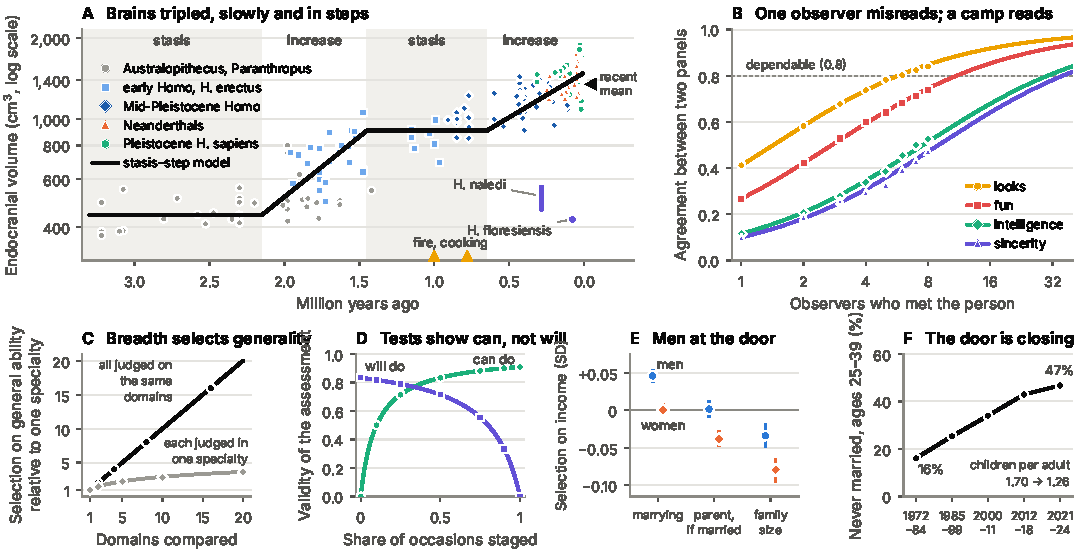
\includegraphics[width=0.93\textwidth]{figures/fig1_main.pdf}\par
\vspace{0pt}
\captionof{figure}{\textbf{The argument in six pictures.} \textbf{(A)}~Endocranial volume of fossil
hominins~\cite{du2018,will2021}, a stasis--step model fitted to \FosN{} other crania~\cite{gingerich2022}, late small-brained
\Homo~\cite{berger2015,kubo2013}, the recent mean~\cite{beals1984}, and earliest secure fire~\cite{berna2012,zohar2022}. \textbf{(B)}~Agreement between two panels of observers about the same person after
four-minute meetings (points; \SdN{} people~\cite{fisman2006}) and the Spearman--Brown law (lines). \textbf{(C)}~Selection on
general ability relative to one specialty (Corollary~\ref{cor:generalist}, Proposition~\ref{prop:division}).
\textbf{(D)}~Validity of 40 observations for what a person can do and will do (Proposition~\ref{prop:staging}).
\textbf{(E)}~Selection on income at three episodes of reproduction, United States, with 95\% intervals ($n=\GssN$).
\textbf{(F)}~Adults aged 25--39 who have never married, United States ($n=\VgBirthN$; Table~\ref{tab:births}).}
\label{fig:main}
\vspace{2pt}
\noindent{\sffamily\scriptsize\color{ink2} Not peer reviewed. Concept and direction: J.~Taylor. Review questions that shaped this version: the authors. Literature synthesis, mathematics, code, data analysis and drafting were AI-assisted (see the disclosure).\par}
\endgroup
\twocolumn

\section{Introduction}\label{sec:intro}

\noindent Hominin endocranial volume roughly tripled across the Plio-Pleistocene, mostly through change within lineages
rather than species turnover~\cite{puschel2024,du2018}. The increase departed from the brain--body scaling of other
primates~\cite{miller2019}, and it was paid for: a child's brain takes about two-thirds of resting metabolism at its
peak~\cite{kuzawa2014}, and human energy budgets exceed those of other apes~\cite{pontzer2016}. Per generation, however, the
change was slow, about $10^{-4}$ standard deviations~\cite{gingerich2022}. Selection that weak is easy to supply. The puzzle
is persistence: why a costly organ kept its direction for some hundred thousand generations, in several lineages, yet not
in all.

One candidate begins with a problem of timing. Much of what a human partner is worth cannot be seen when partners are
chosen. A forager's hunting skill peaks near age 33~\cite{koster2020,gurven2006}, and the number of children a person
raises is not known until middle age, yet marriages are made in the teens and twenties. A capacity that pays at forty and
cannot be seen at twenty is invisible to any selection that works through other people's choices. Humans fill the gap with
performance: foraging, craft, contest, play and speech, repeated in public for years before lifetime outcomes are known.
If prospective partners, their kin and allies used that evidence, and if their decisions changed who reproduced,
information became selection. Nothing in this requires that a bride chose freely; in most recorded societies she did not
(Section~\ref{sec:reschoice}). It requires that whoever decided had watched for years. The idea has a long history in theories of sexual and social
selection~\cite{miller2000ch,miller2000book,hooper2008,westeberhard1983,nesse2007,flinn2005,crespi2022,progovac2026}, and
animal breeders know its logic as a formula: gain per generation equals genetic variation times the accuracy of selection
decisions times their intensity~\cite{lush1937,hazel1943,falconer1996}. Gain rises sharply when accuracy is obtained
early; genomic prediction at birth raised annual gain in dairy cattle by 50--100\%~\cite{garciaruiz2016}. We call the
hypothesis \emph{performance before outcomes}.

The usual test asks whether intelligence is attractive. That question is too coarse to answer, because selection through
mating is a chain of separable links: \emph{who assesses} (a partner, the partner's kin, rivals, allies); \emph{what they
observe} (a cue, a performance, or a record); \emph{how accurately} it forecasts a heritable capacity; \emph{which episode
of reproduction} the decision governs; and \emph{with what aim}, that is, which trait the observation loads on. We take the
chain apart, state each link as a model with proofs and simulation checks, and measure the links that can be measured: in
the fossil record, in a speed-dating experiment, in a national survey followed for fifty years, in the coded ethnographic
record of \CcSccsN{} societies, and in two cross-national surveys of 45 and 175 countries.

Eight results follow. One observer cannot read a mind and a camp can, and people act only on what they can read. Being
judged across many domains aims selection at the generalist. Capacity is selected only where it is delivered, and delivery
cannot be read from a test that the person recognizes: it has to be observed unannounced or enforced by others. The sexes
are selected at different episodes, then and now: men at the door, women after it. The chooser was seldom a free young
woman: parents and elders decide most marriages in the ethnographic record, coercion is common, and the mechanism needs a
jury with years of evidence, not romance or consent. Culture changes the weights on each link without changing the links.
Where a dangerous test is banned a safe, repeatable one takes its place, and keeps what it showed about capacity while
losing what it showed about nerve. And the jury is now being dismissed: Americans want as many children as they did fifty
years ago, and almost all of the shortfall arises before a couple forms. None of this estimates an ancestral parameter.
The paper derives what would have to be true if mate selection contributed to brain expansion, shows which parts hold in
living people, and lists the observations that would count against it. Proofs, simulations, the evidence base and audits
of common claims are in the Supplementary Information (SI).

\section{Results}

\subsection{A slow, persistent, stepwise expansion}\label{sec:resfossil}

We reanalyzed \FosN{} dated crania~\cite{gingerich2022}. Log volume rose by \FosSlopeSpec{} per million years, which is
\FosRateLo--\FosRateHi{}$\times10^{-4}$ standard deviations per generation. A constant trend fits poorly
($\Delta\mathrm{AICc}=\FosAICLin$). The record is better described by stasis broken by two steps, with change points near
\FosBpA, \FosBpB{} and \FosBpC{} million years ago and plateaus at \FosLevI{} and \FosLevIII\ccm{} (Figs.~\ref{fig:main}A
and~\ref{fig:fossils}A), although analyses of cranial shape favor random walks and stasis~\cite{hubbe2026} and stasis
cannot be told from slow change within phases. Over the last 0.9 million years volume rose in three regional series
(Fig.~\ref{fig:fossils}B): by \SerAfr{} log units per million years in the African series leading to \Hs, \SerEur{} in
western Eurasia leading to Neanderthals, and \SerAsia{} in eastern Asia~\cite{will2021}. Neanderthals (\NeaMean\ccm) were
close to contemporaneous \Hs{} (\SapMean\ccm), while two late species kept brains under 600\ccm, the size of an
australopith's, long after the last australopiths had gone: \textit{H.~naledi} in southern Africa about 0.3 million years
ago~\cite{dirks2017}, and \textit{H.~floresiensis} on the island of Flores until some 60,000 years
ago~\cite{sutikna2016} (Fig.~\ref{fig:fossils}C). They lived at the same time as large-brained people, not beside
australopiths and, on Flores, beside no one: the island was reached only by sea, and the lineage was there by 0.7 million
years ago~\cite{brumm2016,vandenbergh2016}. Volume in our own species has not risen for at least 100,000 years, and recent
populations average \RecentDrop\% less than Pleistocene ones~\cite{beals1984}.

What needs explaining is therefore not speed. If the whole increase were a correlated response to selection on a cognitive
capacity, the selection differential required is about $\ReqBase$ standard deviations per generation
(Section~\ref{sec:strength}). The questions are why the direction persisted, why benefits kept pace with rising cost, why
several lineages moved in parallel while others did not, and why change came in steps.

\begin{figure*}[t]
\centering
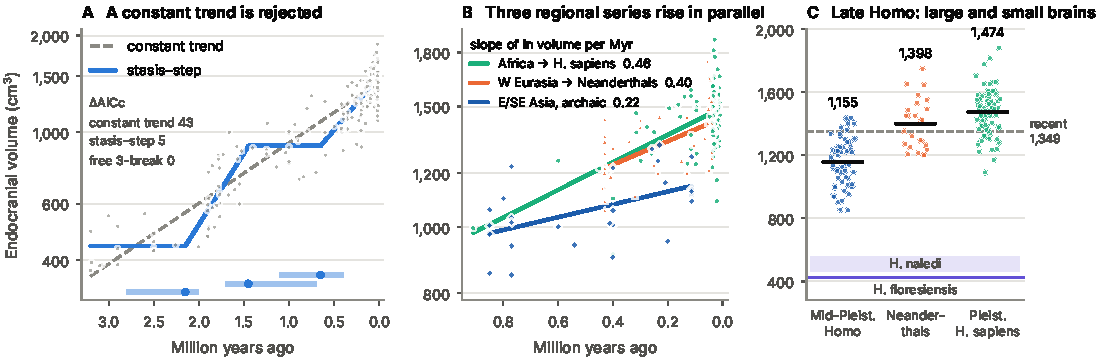
\includegraphics[width=\textwidth]{figures/fig2_fossils.pdf}
\caption{\textbf{The fossil record: slow, stepwise, parallel.} \textbf{(A)}~Endocranial volume of \FosN{} crania~\cite{gingerich2022}
with a constant trend and the stasis--step model; bars at the bottom are bootstrap 95\% intervals for the change points.
\textbf{(B)}~Three regional series over the last 0.9~Myr with fitted slopes~\cite{will2021}. \textbf{(C)}~Late \Homo: specimens and
group means for Middle Pleistocene \Homo, Neanderthals and Pleistocene \Hs~\cite{will2021}; bands mark
\textit{H.~naledi} and \textit{H.~floresiensis}~\cite{berger2015,kubo2013}; the dashed line is the mean of recent
populations~\cite{beals1984}. Claim level: reanalysis of published open data.}
\label{fig:fossils}
\end{figure*}

\subsection{Mate selection has five links}\label{sec:decomp}

The breeder's equation organizes the first three links. If decisions rest on a score $Y$ whose squared correlation with a
capacity is the validity $R$, the response of the capacity's breeding value per generation is
\begin{equation}
S=\sigma_A\cdot h\sqrt R\cdot i,\qquad i=\Corr(Y,W)\,\CV(W),\label{eq:mainidentity}
\end{equation}
genetic standard deviation times accuracy times intensity, where $W$ is reproductive contribution
(Proposition~\ref{prop:identity}). Information enters as $\sqrt R$, so poor information still has an effect, and it is
separable from reproductive inequality: validity can change the response while the distribution of reproduction stays fixed.
\emph{Who assesses} and \emph{what they observe} set $R$. A static cue is read at a glance; a performance has an outcome and
can be repeated; a record accumulates many performances and travels by talk. Parents arrange most marriages in foraging
societies~\cite{walker2011,apostolou2007} and weigh a suitor's investment and cooperation more than their children
do~\cite{buunk2008}; a model with only the partner's choice mistakes one juror for the jury.

The fourth link is the episode. Lifetime reproduction is a sequence, and a selection differential is the sum of the
contributions of its stages~\cite{arnold1984}. For a standardized trait $z$ and completed family size $c$ the split is exact
(Proposition~\ref{prop:episodes}):
\begin{equation}
S=\underbrace{\E[z\mid c>0]}_{\text{access}}+\underbrace{\frac{\Cov(z,c\mid c>0)}{\E[c\mid c>0]}}_{\text{number}}.\label{eq:split}
\end{equation}
Access, becoming a parent at all, is decided largely by other people, though intention, infertility and timing enter it
too. It divides further into pairing and the conversion of a partnership into parenthood. Number depends on timing and on
the stability of unions. Under natural fertility a third term, the survival of children, is at least as
large~\cite{volk2013,sear2008}. Table~\ref{tab:anatomy} sets out the links by sex.

The fifth link is aim. A score loads on some traits more than others, and the loading, not the intensity of competition,
decides what evolves.

\begin{table*}[t]
\caption{The anatomy of mate selection by episode and sex. ``Small-scale societies'' summarizes cited field evidence
(Sections~\ref{sec:evidence} and~\ref{sec:hidden}); ``today'' summarizes Section~\ref{sec:restoday}. Entries describe where trait
variation is converted into reproductive variation; none is an estimate of ancestral selection.}
\label{tab:anatomy}
\scriptsize
\begin{tabularx}{\textwidth}{@{}P{0.115\textwidth}P{0.125\textwidth}LLP{0.205\textwidth}@{}}
\toprule
Episode & Decided mainly by & What varies among men & What varies among women & Today (United States, this paper)\\
\midrule
Access: obtaining a partner and becoming a parent &
Prospective partner; the partner's parents and kin; rivals and allies &
Large. Men's standing predicts reproductive success across 33 societies~\cite{vonrueden2016}; kin arrange most marriages and
apply their own criteria~\cite{walker2011,apostolou2007,apostolou2010}; men's variance in reproductive success usually exceeds
women's~\cite{brown2009,betzig2012}. &
Smaller. Assessed qualities affect \emph{whom} a woman marries (partner quality) more than whether she does; Hadza men
look for hard work and women for intelligence and foraging skill~\cite{marlowe2004}. &
Men: income and standing favored at pairing; childlessness concentrated at the bottom of the income distribution. Women: no
effect at pairing over the whole period; schooling, standing and income lower the chance of motherhood
(Tables~\ref{tab:gss} and~\ref{tab:funnel}).\\
\addlinespace
Timing: age at first birth &
The couple and their kin &
Prestigious Tsimane men marry wives who first give birth at younger ages, the strongest path from status to fitness
there~\cite{vonrueden2011}. &
Earlier first birth lengthens the reproductive span. &
Later first birth, which goes with more schooling, accounts for \GssTimShareW\% (women) and \GssTimShareM\% (men) of the
schooling--family-size relation among parents.\\
\addlinespace
Number: births while partnered; remarriage, polygyny &
The couple; rivals for additional partners &
Serial marriage raised men's number in the United States and polygyny did in nineteenth-century
Utah~\cite{jokela2010,moorad2011}. Among Pimbwe, once years married are held constant, extra partners help women and not
men~\cite{borgerhoffmulder2019}. &
Birth spacing, limited by energy and help. Extra husbands added little in the United States and Utah
samples~\cite{jokela2010,moorad2011}. &
Negative association with schooling, vocabulary and standing in both sexes; a second marriage adds children for men
only; more sexual partners go with fewer children.\\
\addlinespace
Survival of off\-spring &
The mother; allomothers; the father's provisioning &
Provisioning and protection. Prestigious Tsimane men have lower offspring mortality~\cite{vonrueden2011}; which relatives
improve child survival varies among societies~\cite{sear2008}. &
Large. A mother's knowledge~\cite{mcdade2007}, standing~\cite{alami2020} and kin help~\cite{sear2008} predict child health and
survival. &
Negligible variance: nearly all children survive.\\
\bottomrule
\end{tabularx}
\end{table*}

\emph{The assessor need not be the bride, and the choice need not be free.} The identity holds for any assessor. If a
share $\kappa$ of matings is settled without regard to the assessed trait, by capture or coercion, the differential on
that trait is
\begin{equation}
S=(1-\kappa)\,S_{\text{assessed}}+\kappa\,S_{\text{force}},\label{eq:coercion}
\end{equation}
where $S_{\text{force}}$ is whatever a contest of force selects, which is the body (Section~\ref{sec:rescontest}).
Coercion subtracts from the pathway in proportion to its share and puts selection on formidability in its place
(simulation: largest error \NtCoeErr). Section~\ref{sec:reschoice} reports what the ethnographic record codes about who
the assessor was and about $\kappa$.

\subsection{One observer cannot read a mind; a camp can}\label{sec:resjury}

How much does one meeting reveal, and how fast do observers converge? In the Columbia speed-dating
experiment~\cite{fisman2006}, \SdN{} graduate students met in \SdSessions{} sessions; each pair talked for four minutes,
rated the other on six attributes and said yes or no to meeting again (\SdRows{} meetings; Methods). Two observers of the
same person agree \JurOneAtt{} about looks and \JurOneFun{} about how much fun someone is, but only \JurOneInt,
\JurOneAmb{} and \JurOneSin{} about intelligence, ambition and sincerity. Agreement between two panels of $k$ observers
then rises as the Spearman--Brown law requires~\cite{spearman1910,brown1910},
\begin{equation}
r_k=\frac{k\,r_1}{1+(k-1)\,r_1},\label{eq:sb}
\end{equation}
to within \JurGapMax{} at every panel size we could test (Fig.~\ref{fig:main}B). A dependable verdict ($r_k=0.8$) takes
\JurKAtt{} observers for looks, \JurKFun{} for fun, \JurKInt{} for intelligence and \JurKSin{} for sincerity. A suitor
cannot read a mind in an evening. A camp of a few dozen people~\cite{hill2011} that has watched someone for years can.
The gain comes only from independent observation. If observers share a fraction $c$ of their error, as people repeating
one report do, their consensus grows while its accuracy cannot exceed $r_1/[r_1+c(1-r_1)]$: \JurCeil{} for a trait read as
poorly as intelligence, at $c=0.3$ (Section~\ref{sec:speed}).
Asking does not help: self-ratings of intelligence and sincerity correlate \SdSelfInt{} and \SdSelfSin{} with the panel's
verdict. Nor is the verdict mere consensus: the panel's rating of intelligence, and not of looks, tracks the median
entrance-test score of the person's college ($r=\SdSat$; \SdSatCI; $n=\SdSatN$).

\emph{People act on what they can read.} Before the event women gave most weight to intelligence and sincerity, and men to
looks and then intelligence. What earned a yes was looks above all, in both sexes, then shared interests and fun;
intelligence earned little, sincerity and ambition nothing (Fig.~\ref{fig:jury}A). The sexes differ less in what they do
than in what they say~\cite{eastwick2014,eastwick2025}: men respond more to looks (by \SdRevDiffAtt{} points per standard
deviation; \SdRevDiffAttCI) and women slightly more to intelligence (\SdRevDiffInt; \SdRevDiffIntCI), as the original
authors found~\cite{fisman2006}, but the profiles have one shape. That shape is the order in which four minutes can read
the attributes ($r=\SdLegPear$ between agreement and effect across the five personal attributes; Fig.~\ref{fig:jury}B).
With five attributes this cannot separate legibility from taste (prediction P27), but it is what the theory requires: a
preference is only as strong as the instrument that serves it. Societies that select on mind and character must possess
instruments that read them.

\emph{Access is unequal within minutes, and misjudged.} Women said yes to \SdYesW\% of partners and men to \SdYesM\%;
\SdPopZeroM\% of men and \SdPopZeroW\% of women received no yes at all. Each sex expected a yes from \SdExpW\% of partners.
Women received one from \SdActW\% and men from \SdActM\%: men overestimated their welcome by \SdGapM{} points (\SdGapMCI)
and women did not (Fig.~\ref{fig:jury}C), the asymmetry that error-management theory
predicts~\cite{haselton2000,perilloux2012}. Neither sex knew which partners had said yes (correlations of \SdAccM{} and
\SdAccW{} between guess and outcome).

\begin{figure*}[t]
\centering
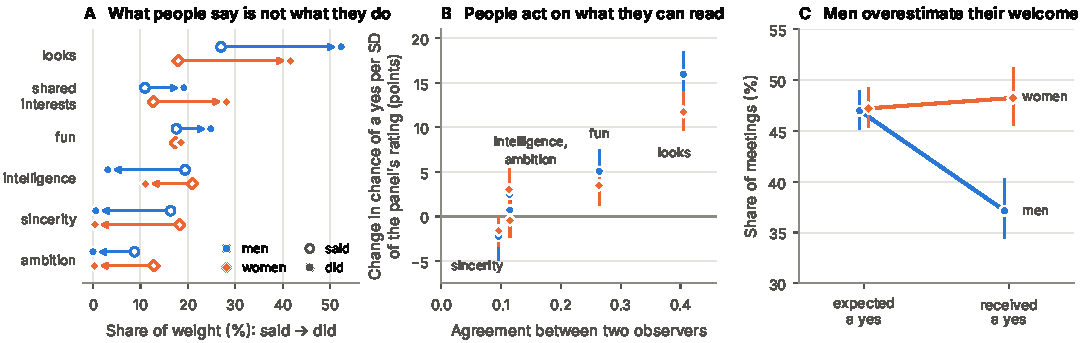
\includegraphics[width=\textwidth]{figures/fig3_jury.pdf}
\caption{\textbf{Said, done, and what four minutes can read.} Columbia speed-dating experiment~\cite{fisman2006}: \SdN{}
people, \SdRows{} meetings; men are circles and women diamonds; whiskers are 95\% bootstrap intervals. \textbf{(A)}~For each
attribute, the share of 100 points given to it before the event (open markers) and its share of the summed positive
effects on a yes (filled markers); arrows run from said to did. \textbf{(B)}~Change in the probability of a yes per standard
deviation of everyone else's rating of the partner, against the agreement between two observers of the same person.
\textbf{(C)}~Share of meetings in which a person expected a yes (the 1--10 guess rescaled to 0--100) and in which a yes was
received. Claim level: reanalysis of public data.}
\label{fig:jury}
\end{figure*}

\emph{Night talk and long acquaintance.} Published results show the same thing outside the laboratory. Among 167
couples, those who had known each other longer before dating were less alike in rated attractiveness: agreement about who
is desirable is strongest early in acquaintance and gives way as people learn what a glance cannot
show~\cite{hunt2015}. Two-thirds of adults in seven samples said their romance began as a
friendship~\cite{stinson2022}. The forager's instrument for this was the evening. Among the Ju/'hoansi, talk by day was
of practical matters and complaints about others, and talk by firelight was stories~\cite{wiessner2014}; people in three
societies without electricity fall asleep 3.3 hours after sunset on average~\cite{yetish2015}. Fire lengthened the day
for observation as well as for digestion~\cite{dunbar2014}. It added occasions, an audience, and a domain, speech, on
which everyone present could be compared. The payoffs are measurable in living foragers: skilled Agta storytellers are
preferred as camp-mates and have more surviving children~\cite{smith2017}; Agta and BaYaka mothers who are better
connected in the camp's network of contacts have more living offspring~\cite{page2017}; and BaYaka with more partners in
cooperation are better nourished, the women more fertile~\cite{chaudhary2016}.

\subsection{Breadth aims selection at the generalist}\label{sec:resgeneralist}

Let performance in each of $K$ domains be the sum of a general capacity $G$ and a domain-specific one, and let standing
depend on the average across domains. Then the selection differential on general capacity relative to that on any one
specialty is
\begin{equation}
\frac{S_{A_G}}{S_{A_{S_k}}}=K\,\frac{V_{A,G}}{V_{A,S}}\label{eq:mainaim}
\end{equation}
(Corollary~\ref{cor:generalist}; Fig.~\ref{fig:main}C). One venue cannot tell a generalist from a specialist. Each added venue
dilutes every specialty and leaves the pull on what the venues share undiminished. Four further results sharpen this.

\emph{Breadth buys time.} With few domains, no amount of watching reaches a given accuracy for general capacity, because
domain-specific ability and persistent error never average out; with many, a little evidence from each suffices
(Proposition~\ref{prop:time}; Fig.~\ref{fig:polymath}A). Mastery of any one demanding skill arrives late, so a specialist's
quality is known late. A generalist's can be known early, from how a young person does in many things, including how
quickly new ones are picked up. Performance before outcomes is feasible for general capacity in a way that it is not for a
single skill.

\emph{Expenditure follows breadth.} If general capacity costs $c_G$ per unit and specific skill $c_S$, the share of
investment devoted to general capacity at equilibrium is $Kc_S/(Kc_S+c_G)$, which passes one half when the number of commonly
assessed domains equals the cost ratio (Proposition~\ref{prop:polymath}; Fig.~\ref{fig:polymath}B). General capacity is the
expensive kind if it resides in tissue serving every domain, so a lineage with a narrow repertoire should invest in
specialized skill however intense its competition, and one with a broad repertoire in general capacity. Cumulative culture
adds domains, which ties the demand for a general-purpose brain to the breadth of culture and not to its depth.

\emph{Breadth taxes show.} Inflating one performance moves a $K$-domain average by $1/K$ of the inflation, while general
capacity moves it in full, so common comparison dilutes exaggeration exactly as it dilutes specialty, without requiring
that display be costly (Corollary~\ref{cor:inflation}; Fig.~\ref{fig:polymath}C). What it cannot dilute is a talent for
seeming that carries across every venue.

\emph{Division of labor restores the specialist.} If each person performs, and is compared, only in the domain of their
greatest talent, the aim on general capacity weakens by a factor $Kc_K$, where $c_K$ is the variance of the largest of $K$
standard normal variables: \PolyDivFive-fold for five domains and \PolyDivTen-fold for ten (Proposition~\ref{prop:division};
grey line in Fig.~\ref{fig:main}C). What removes the generalist aim is the loss of a common set of domains, not esteem for
excellence.

The conditions for the generalist aim were met in small societies without occupational specialization. Tsimane adults
command a broad repertoire across food production, child care, craft, music and storytelling, most of it before first
reproduction~\cite{schniter2015}. The general factor has biological standing: across 62 primate species, innovation,
social learning, tool use and extractive foraging form one composite that covaries with brain volume~\cite{reader2011}; most
genetic influences on human cognitive abilities are shared across abilities~\cite{kovas2006,plomin2015}; and the cortex that
expanded most in our lineage is association cortex~\cite{hill2010,buckner2013}, recruited by demanding tasks of every
kind~\cite{duncan2010}. Two cautions apply. A portfolio rewards whatever is common to all venues, which includes health,
condition and opportunity as well as cognition. And the argument shows what such selection would favor, not that it
occurred.

\begin{figure*}[t]
\centering
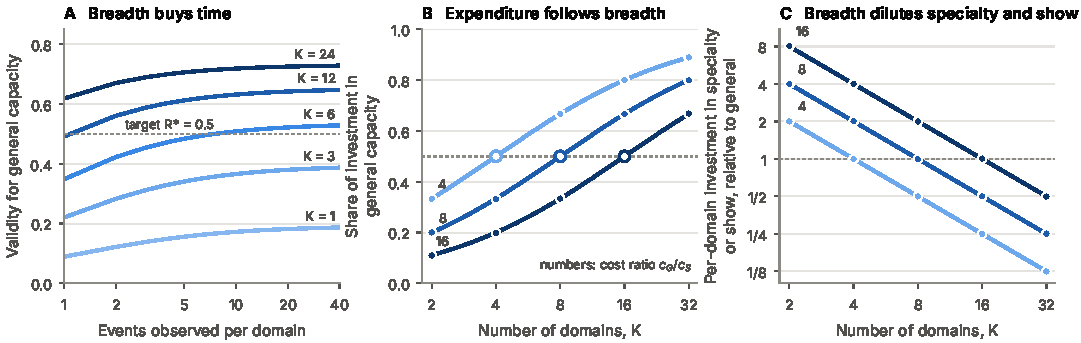
\includegraphics[width=\textwidth]{figures/fig4_polymath.pdf}
\caption{\textbf{Selecting the generalist.} \textbf{(A)}~Breadth buys time: validity for general capacity against events observed
per domain, for 1 to 24 domains (Eq.~\ref{eq:RG}); the dashed line is the target $R^*=0.5$, reached only with more than
five domains (Proposition~\ref{prop:time}). \textbf{(B)}~Expenditure follows breadth: share of investment cost devoted to general
capacity at evolutionary equilibrium, for three ratios of the cost of general to specific capacity; curves are
Eq.~\eqref{eq:share}, markers individual-based simulations, and open circles mark the threshold $K^\dagger=c_G/c_S$.
\textbf{(C)}~Breadth dilutes specialty and show: equilibrium investment per domain in a specific skill, or in exaggerating one
performance at the same cost, relative to investment in general capacity (lines: Eq.~\ref{eq:gstar}; markers: the same
simulations). Parameters are illustrative (Table~\ref{tab:experiments}). Claim level: exact results with numerical checks.}
\label{fig:polymath}
\end{figure*}

\subsection{Contests of force select the body}\label{sec:rescontest}

Popular accounts give fighting the leading role. A contest of force loads on formidability. In the model, moving the basis
of standing from dominance to prestige raises selection on general capacity \AimGain-fold and lowers selection on
formidability \AimLoss-fold at the same intensity (Proposition~\ref{prop:aim}). The comparative record agrees: across primates,
stronger male contest goes with dimorphism in body and canine size~\cite{plavcan2012} and not with larger
brains~\cite{schillaci2006,lemaitre2009,fitzpatrick2012}. Contest contributed to the mind indirectly. Restraint makes contests
repeatable, and repetition is information: validity rises from \RepROne{} for a single decisive fight toward \RepRsafe{} when
bouts are cheap enough to hold nineteen (Proposition~\ref{prop:repeat}). And strong rival coalitions make it rational even for
a dominant to share reproduction (Proposition~\ref{prop:despot}), which lowers intensity \DesIntLo- to \DesIntHi-fold while
moving the criterion of standing from force toward esteem conferred by others~\cite{boehm1993,wrangham2018}. Leveling slows
selection and re-aims it.

\emph{When a dangerous test is banned, a safe one takes its place.} Games with a winner and a loser are recorded in
\CcGamesAny{} of \CcGamesN{} societies with data~\cite{roberts1959,kirby2016}. Men who take part in Sereer ritual
wrestling have more children, although women rank wrestling low among the qualities they say they
want~\cite{llaurens2009}: the verdict of a public contest is used by someone other than the bride. A current case shows
the substitution as it happens. A Maasai warrior once proved himself by killing a lion. With lions scarce and the hunt
illegal, elders conceived in 2008, and first held in 2012, a tournament of running, throwing and a standing high jump
modeled on the warriors' jumping dance, to stand in for the hunt as the mark of manhood, bravery and
prestige~\cite{maasaiolympics,aljazeera2022,hazzah2009,goldman2013}. A man may by custom marry only after the ceremony
that ends warriorhood~\cite{aljazeera2023,spencer1988}; we found no source that makes the height of a jump a condition of
marriage, and standing, not eligibility, is what the jump confers. The theory says what such a change keeps and what it
loses. For capacity it loses nothing: $n$ repetitions of a safe trial of reliability $\rho_s$ match one dangerous trial
of reliability $\rho_d$ once
\begin{equation}
n\ \ge\ \frac{\rho_d\,(1-\rho_s)}{\rho_s\,(1-\rho_d)}\label{eq:ritual}
\end{equation}
(Corollary~\ref{cor:ritual}), which is \NtRitA{} jumps when one jump tells a fifth as much as the hunt, and the whole
community can watch each of them. For willingness to face real danger it loses everything, because a tournament is a
recognized test (Section~\ref{sec:resverify}). That has to be read elsewhere, in years of herding and of service to the
age-set. Safe, repeatable rituals are how a society keeps reading capacity when it can no longer afford the price of the
old test.

\subsection{Capacity is selected only where it is delivered}\label{sec:resdelivery}

A partner's capacity is worth nothing to a chooser unless its product arrives. Let $b$ be the benefit a candidate can
produce and $p$ the share that reaches the chooser and the chooser's children. With value $pb$, the selection differentials
on the two traits are $S_{A_B}\propto\bar p\,R_b$ and $S_{A_P}\propto\bar b\,R_p$ (Proposition~\ref{prop:delivery}). Where
partners deliver nothing, choice for benefits puts no selection on capacity, however able the candidates. The two traits
are complements, so capacity and commitment rise together or not at all, and the take-off has a threshold. And the two
are known through different evidence: capacity shows in performance, which is public and quick; delivery shows in conduct
when interests conflict, which is private and slow.

Present-day evidence fits the distinction. Warmth and trustworthiness form a factor of partner ideals separate from
attractiveness and from status~\cite{fletcher1999}; kindness behaves as a necessity in both sexes~\cite{li2002}; a partner's
perceived commitment and appreciation predict the quality of a relationship where the partner's traits add
nothing~\cite{joel2020}; responsiveness raises desire~\cite{birnbaum2016}; and about two-thirds of relationships in seven
samples began as friendships~\cite{stinson2022}. Human paternal investment, unusual among
mammals~\cite{geary2000,marlowe2000}, is what makes $\bar p$ large enough for the rest of the mechanism to matter.

\subsection{A test shows what a person can do, not what the person will do}\label{sec:resverify}

A candidate who knows when assessment is taking place can change what it shows, and capacity and delivery respond in
opposite ways. Capacity cannot be displayed beyond its level, so the occasions on which a person tries hardest are the best
evidence of it. Delivery is a choice, so an occasion known to be a test says nothing about what will be chosen later. If a
share $d$ of $n$ observed occasions is recognizable as assessment, the validities for capacity and delivery are
\begin{equation}
R_b=\frac{V_B}{V_B+\sigma^2/(dn)},\qquad R_p=\frac{V_P}{V_P+\nu/[(1-d)n]}\label{eq:mainstaging}
\end{equation}
(Proposition~\ref{prop:staging}; Fig.~\ref{fig:main}D). Only occasions that cannot be told from ordinary life inform an
assessor about delivery, and after $m$ of them without a default the default rate is bounded only by about $3/m$:
reliability is never established, only not yet refuted. The speed-dating data show the limit case. A four-minute date is
all test, and sincerity is the attribute it reads worst and rewards least (Fig.~\ref{fig:jury}B). People reason as the
result requires. They ask first whether another person intends good or ill and then whether that person can act on the
intention~\cite{fiske2007}; they weigh good performances more heavily in judging competence and bad conduct more heavily in
judging character~\cite{reeder1979,wojciszke1993}; and maximum and typical performance correlate only
moderately~\cite{beus2012}. Display also bends toward its audience: single women in a business school reported lower
desired salaries and less willingness to travel when single male classmates would see their answers, and no less when the
answers were private~\cite{bursztyn2017}. The practices that add unstaged observation are familiar: long acquaintance
before commitment~\cite{wachtmeister1999,seymour2009,stinson2022}, brideservice under the eyes of
in-laws~\cite{walker2011}, life in a group small enough that conduct is seen daily, and reports from people whose
interests differ from the candidate's.

The alternative to verifying a disposition is to make it matter less. If third parties enforce delivery of a share $e$ of
every candidate's product, as foragers' norms of sharing do~\cite{woodburn1982,peterson1993,wiessner2005}, capacity is
selected in proportion to $e+(1-e)\bar p$ and commitment in proportion to $1-e$ (Proposition~\ref{prop:enforce}).
Enforcement therefore removes the take-off threshold: capacity is selected from the outset, with no evolved commitment at
all (Fig.~\ref{fig:verify}A). It also hides disposition from selection, so evolved commitment is greatest under partial
enforcement, and where choice alone would have sufficed, enforcement crowds commitment out and can lower what is
delivered in all (Fig.~\ref{fig:verify}B). On this reading leveling did more than change the criterion of standing
(Section~\ref{sec:rescontest}): by enforcing delivery it made capacity worth choosing before commitment had evolved. As
history that order is conjecture.

\begin{figure*}[t]
\centering
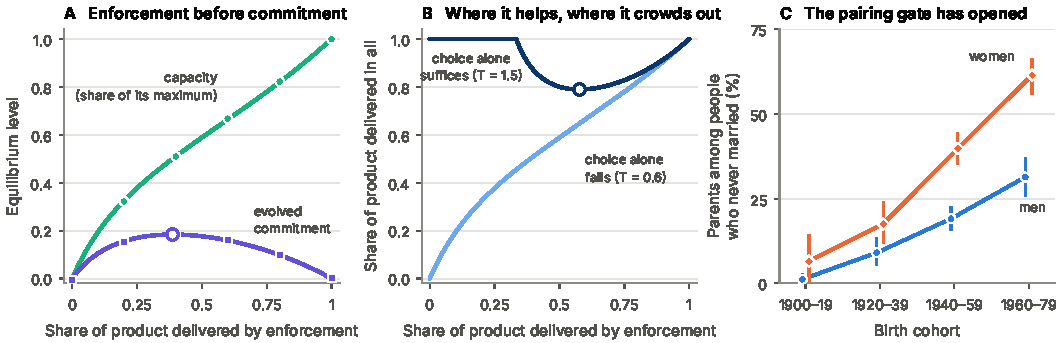
\includegraphics[width=\textwidth]{figures/fig5_verify.pdf}
\caption{\textbf{Enforcement, and a gate.} \textbf{(A)}~Equilibrium capacity, as a share of its maximum, and evolved commitment
against the share of product whose delivery third parties enforce, when choice alone is below the take-off threshold
($T=\EnfT$; Proposition~\ref{prop:enforce}); lines: exact; markers: individual-based simulation; the open circle marks the
peak of commitment. \textbf{(B)}~Share of product delivered in all, enforced plus volunteered, below the threshold ($T=\EnfT$)
and above it ($T=\EnfCrowdT$), where enforcement lowers delivery to a minimum of \EnfCrowdMin{} (open circle).
\textbf{(C)}~Among people who never married, the percentage who are parents, by birth cohort and sex, United States General
Social Survey, ages 45--79; whiskers are 95\% bootstrap intervals; men are circles and women diamonds. Parameters in A and
B are illustrative (Table~\ref{tab:experiments}). Claim level: A and B, exact results with numerical checks; C, reanalysis
of public data~\cite{gss2024}.}
\label{fig:verify}
\end{figure*}

\subsection{Men are selected at the door, women after it}\label{sec:ressexes}

In small-scale and historical societies the episode differs by sex (Table~\ref{tab:anatomy}). For men it is access. Men's
standing predicts reproductive success across 33 societies~\cite{vonrueden2016}; men's variance in reproductive success
usually exceeds women's~\cite{brown2009,betzig2012}; and in a Finnish population with every episode recorded, variance in mating
success explained most of men's excess variance in fitness~\cite{courtiol2012}. For women it is the survival of children and
the timing of the first birth. A Tsimane mother's plant knowledge predicts her children's health~\cite{mcdade2007}, her
political influence predicts their growth and freedom from illness~\cite{alami2020}, relatives improve child survival in
almost every population studied~\cite{sear2008}, and prestigious men gain chiefly through wives who start
earlier~\cite{vonrueden2011}. Selection on women's competence and social skill did not need anyone's choice of them. Cognition
is nonetheless similar in the two sexes, as shared inheritance guarantees whichever sex is selected~\cite{lande1980}.

\label{sec:restoday}Present-day data cannot show what happened in the Pleistocene, but they show which features of human
mate selection persist when fertility is controlled. We applied Eq.~\eqref{eq:split} to \GssN{} adults aged 45--79 in the
United States General Social Survey~\cite{gss2024}, for four traits standardized within sex and birth decade
(Table~\ref{tab:gss}; Methods).

\emph{Number runs against every trait in both sexes.} Among parents, more schooling, a larger vocabulary, a more
prestigious occupation and a higher income go with fewer children. Later first births account for \GssTimShareW\% of the
relation with schooling among mothers and \GssTimShareM\% among fathers.

\emph{Access has opposite signs in the two sexes.} For income the access component is \GssIncMAcc{} (\GssIncMAccCI) in men and
\GssIncWAcc{} (\GssIncWAccCI) in women. For men the two episodes cancel, leaving a total near zero: what pairing rewards,
family size takes back, and a single correlation between status and fertility would report no selection where there are
two opposed episodes.

\emph{For men the door is marriage, and it is a floor.} Splitting access into pairing (ever marrying) and conversion
(parenthood given pairing) puts all of men's advantage at the first step: \GssIncMPair{} (\GssIncMPairCI) for income at
pairing and \GssIncMConv{} at conversion (Fig.~\ref{fig:main}E; Table~\ref{tab:funnel}). Occupational standing, schooling
and vocabulary are also positive at pairing in men. Childlessness falls from \GssQfMOne\% in the lowest fifth of men's
income to \GssQfMThree\% in the middle fifth and \GssQfMFive\% in the highest (Fig.~\ref{fig:today}A); \GssNmMOne\% of men
in the lowest fifth never married, against \GssNmMFive\% in the highest, and the gradient is concentrated at the bottom
(difference in differences \GssFloorM{} percentage points; \GssFloorMCI). Standing buys a man a marriage, not more partners
and not more children: the rank correlation between a man's income and his lifetime number of sexual partners is
\GssPartIncM{} (\GssPartIncMCI), and family size is highest for people reporting one lifetime partner
(Fig.~\ref{fig:today}C).

\emph{For women the selection comes after the door.} Pooled over cohorts, no trait has a detectable effect on whether a
woman marries (income: \GssIncWPair; \GssIncWPairCI); the negative access component arises at conversion (\GssIncWConv),
and childlessness rises from \GssQfWOne\% to \GssQfWFive\% across fifths of women's income. In women born 1960--1979 the
sign at the door has turned: higher income now goes with marrying (\GssPairWNew; \GssPairWNewCI), while its relation to
motherhood within marriage has grown more negative (\GssConvWNew; \GssConvWNewCI). The same trait is now favored at the
door and disfavored after it.

\emph{Leaving and re-entering a marriage pays men only.} Relative to people of their sex and birth decade in a first
marriage, remarried men have \GssRemM{} more children (\GssRemMCI) and remarried women \GssRemW{} (\GssRemWCI); men who
divorced and did not remarry have \GssDivM{} (\GssDivMCI) and such women \GssDivW{} (Fig.~\ref{fig:today}F), as serial
marriage does elsewhere~\cite{jokela2010}.

\emph{The gate passes less and selects more.} Selection at pairing can act only on reproduction that passes through
pairing. Among people born 1920--1939, \GssGateMOld\% of never-married men and \GssGateWOld\% of never-married women were
parents; among those born 1960--1979 the figures are \GssGateMNew\% and \GssGateWNew\% (Fig.~\ref{fig:verify}C). Over the
same cohorts the share of men never marrying rose from \GssNevMOld\% to \GssNevMNew\% and the pairing differential on
men's income rose from \GssPairMOld{} to \GssPairMNew{} (change \GssPairMChange; \GssPairMChangeCI;
Table~\ref{tab:gssgate}). Who marries whom changed too: wives had more schooling than their husbands in \GssHypMoreMid\% of
marriages of people born 1940--1959 and less in \GssHypLessMid\%; for those born from 1980 the figures are
\GssHypMoreYoung\% and \GssHypLessYoung\%, the reversal seen worldwide~\cite{esteve2016}. Many births outside marriage are
to cohabiting couples~\cite{lundberg2016}, so these figures describe marriage, not partnership. Meanwhile access has
tightened at younger ages: at 22--34 the share with no sexual partner in the past year rose from \GssPlMOld\% to
\GssPlMNew\% among men and from \GssPlWOld\% to \GssPlWNew\% among women between 1989--2002 and 2016--2024, and it is graded
by income in both sexes (Fig.~\ref{fig:today}D; Table~\ref{tab:funnel})~\cite{ueda2020}. Childlessness now carries
\GssShareMNew\% of the opportunity for selection among men and \GssShareWNew\% among women born 1960--1979, up from
\GssShareMOld\% and \GssShareWOld\% in those born 1920--1939 (Fig.~\ref{fig:today}E).

These patterns replicate and extend earlier reports. Low-income men are more often childless in Britain, Sweden, the Nordic
countries and the United States, while the relation for women is negative or
reversing~\cite{nettle2008,fieder2007,barthold2012,hopcroft2021,weeden2006,kolk2023,jalovaara2019,kolk2019}. In the Nordic countries the
negative gradient of women's education has vanished~\cite{jalovaara2019}, so the sign for women tracks institutions; the
positive sign for men is found wherever it has been sought. Genetic evidence points the same way. Scores for educational
attainment are negatively associated with number of children, largely through timing~\cite{kong2017,beauchamp2016,hughjones2022},
and carriers of rare damaging variants are more often childless, men especially, apparently for want of a
partner~\cite{gardner2022}. The differentials here are phenotypic, from one country, and self-reported; income is partly a
consequence of family formation~\cite{kleven2019}; the cohort comparisons were not planned in advance; and nothing in them
bears on the worth of any person or group (Section~\ref{sec:gss}).

\begin{table*}[t]
\caption{Selection differentials in a present-day population, split into access and number (Eq.~\ref{eq:split}). United States,
General Social Survey 1972--2024, ages 45--79, cohorts 1900--1979. Units: standard deviations of the trait per generation;
95\% bootstrap intervals in brackets.}\label{tab:gss}
\footnotesize
\begin{tabularx}{\textwidth}{@{}P{0.19\textwidth}lrCCC@{}}
\toprule
\tabinput{generated/tab_gss.tex}
\bottomrule
\end{tabularx}
\tablenote{Access is the mean standardized trait among parents; number is the covariance of the trait with family size among
parents divided by their mean family size; the two sum to the total. Traits are standardized, and fitness is relative, within
sex and decade of birth. Income is measured at ages 45--64. Phenotypic differentials, not genetic responses. Claim level:
reanalysis.}
\end{table*}

\begin{table*}[t]
\caption{Seven steps on the path to parenthood, by sex: where a higher income, or a marriage, pays. United States, General
Social Survey; ages 45--79 unless stated; 95\% bootstrap intervals in brackets.}\label{tab:funnel}
\footnotesize
\begin{tabularx}{\textwidth}{@{}P{0.135\textwidth}LP{0.2\textwidth}P{0.2\textwidth}@{}}
\toprule
\tabinput{generated/tab_funnel.tex}
\bottomrule
\end{tabularx}
\tablenote{The three differentials are computed among respondents whose marital status is known, so the number component
differs in the third decimal from Table~\ref{tab:gss}. Family size in the last two rows is relative to the mean of the
respondent's sex and decade of birth, and the comparison is with people in a first marriage who never divorced. None of
the rows is causal.}
\end{table*}

\begin{figure*}[t]
\centering
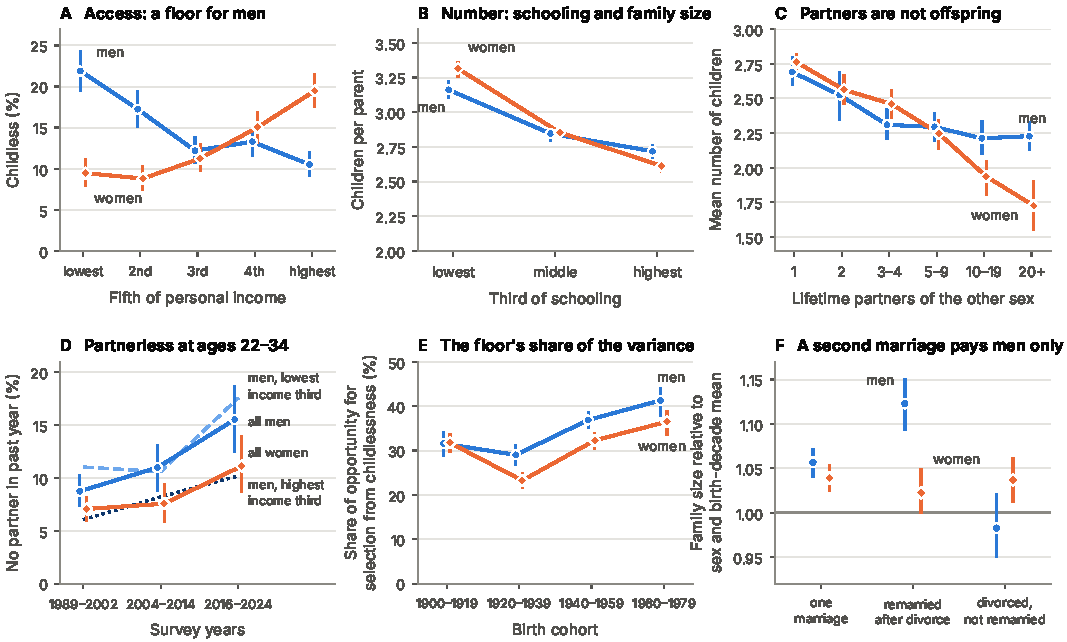
\includegraphics[width=\textwidth]{figures/fig6_today.pdf}
\caption{\textbf{Where selection sits in a present-day population.} United States, General Social Survey 1972--2024, adults aged
45--79 born 1900--1979 (panel D: ages 22--34); whiskers are 95\% bootstrap intervals; men are circles and women diamonds.
\textbf{(A)}~Percentage childless by fifth of personal income within sex and birth decade: a floor for men, and a rise at the
top for women. \textbf{(B)}~Mean number of children among parents by third of schooling. \textbf{(C)}~Mean number of children by
reported lifetime number of opposite-sex partners since age 18; the category of no partners is omitted because it contains
inconsistent reports. \textbf{(D)}~Percentage reporting no sexual partner in the past year, by period; dashed and dotted lines
are men in the lowest and highest thirds of own income, shown without intervals. \textbf{(E)}~Share of the opportunity for
selection that is due to childlessness (Eq.~\ref{eq:oppsplit}), by birth cohort. \textbf{(F)}~Family size by marital history,
relative to the mean of the respondent's sex and decade of birth. Source: authors' analysis of public
data~\cite{gss2024}.}
\label{fig:today}
\end{figure*}

\emph{The door in 70 countries.} A survey of \WdN{} people in 175 countries~\cite{kowal2025} allows a test outside the
United States, with self-ratings in place of records. Within country and sex, and holding age fixed, a standard deviation
of a man's rating of his own financial prospects goes with \WdDoorResM{} percentage points in the probability that he has
a partner (\WdDoorResMCI). For a woman the figure is \WdDoorResW{} (\WdDoorResWCI), and the difference is \WdDoorResDiff{}
points (\WdDoorResDiffCI; \WdDoorN{} people in \WdCtry{} countries with at least fifty of each sex;
Fig.~\ref{fig:world}C). Men's coefficient exceeds women's in \WdDoorCtryPos{} of the \WdDoorCtry{} countries with enough
respondents to estimate each. Looks go with having a partner in both sexes (\WdDoorLooksM{} and \WdDoorLooksW{} points).
Self-rated kindness goes with nothing (\WdDoorKindM{} and \WdDoorKindW), though kindness is what both sexes say they want
most (Section~\ref{sec:resculture}). These are cross-sectional self-reports, and having a partner may itself raise a man's
view of his prospects.

\emph{Who becomes an ancestor.} A popular reading of the genetic record holds that twice as many women as men left
descendants, or that only half of all men ever fathered a child~\cite{baumeister2010}. The observation behind it is sound.
Mitochondrial lineages coalesce about twice as deep as Y-chromosome lineages in each of three
populations~\cite{wilder2004}, and comparisons of maternal, paternal and X-linked diversity point the same
way~\cite{hammer2008,lippold2014}. The reading is not. Such data estimate a ratio of effective numbers, and for a sex in
which a share $q$ leaves no offspring and family size among the rest has mean $m$ and variance $m+\alpha m^2$,
\begin{equation}
\frac{N_e}{N}=\frac{1-q}{1+\alpha}\label{eq:ancestors}
\end{equation}
whatever the mean (Proposition~\ref{prop:ancestors}; simulation within \NtAncErr\%). A twofold ratio follows if 80\% of
women and 40\% of men reproduce and parents of each sex are otherwise alike. It follows equally if the same share of each
sex reproduces and fathers differ among themselves as much as $\alpha=1$ implies, as under polygyny, and competition among
patrilineal clans produces it with no difference in headcounts at all~\cite{zeng2018,karmin2015}
(Fig.~\ref{fig:choice}D). Nor does a lineage hold twice as much female DNA: mother and father contribute equally to every
child's other chromosomes. In the United States the two effective numbers are nearly equal, \VgNeM{} of the census number
for men and \VgNeW{} for women born 1900--1979, a ratio of \VgNeRatio{} (\VgNeRatioCI). The ratio has risen to
\VgNeRatioNew{} (\VgNeRatioNewCI) among those born 1960--1979, as men's childlessness reached \VgQMNew\% against women's
\VgQWNew\%. What the genetic ratio does establish is that men's reproduction was the more unequal for a very long time.
That is the condition under which a floor at the door selects: excluding 40\% of men puts an intensity of \NtIqForty{}
standard deviations on whatever admits the rest (Corollary~\ref{cor:floor}); the \VgQM\% excluded in the United States
puts \NtIqUS.

\subsection{A jury chose, and the bride was often not asked}\label{sec:reschoice}

\begin{figure*}[t]
\centering
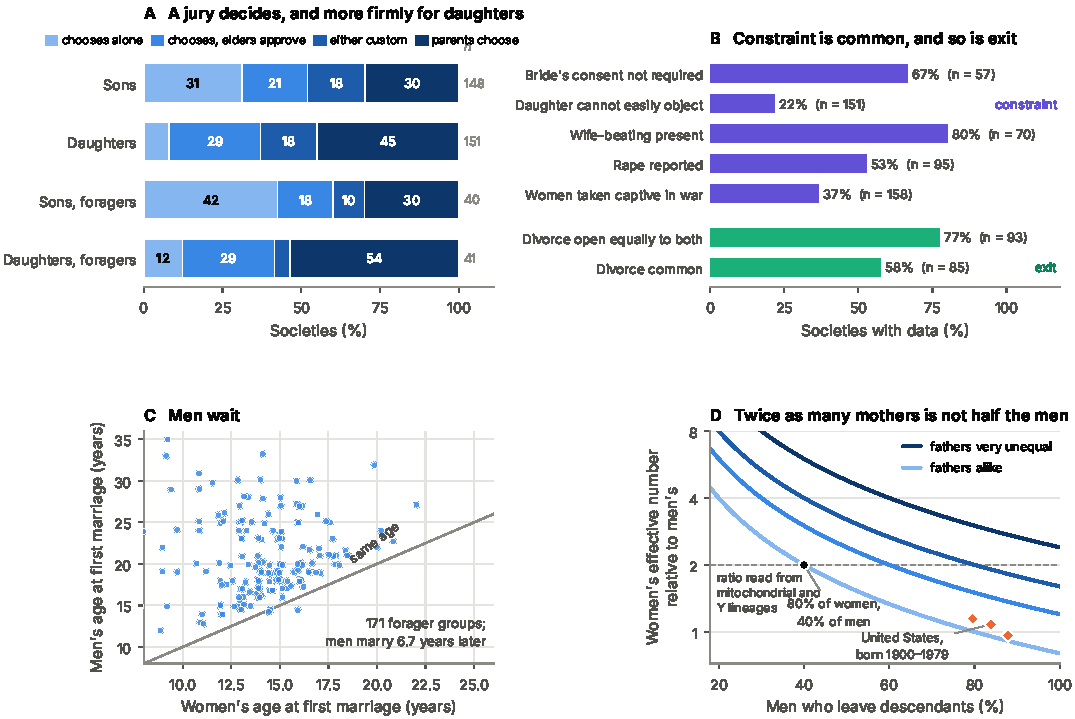
\includegraphics[width=\textwidth]{figures/fig7_choice.pdf}
\caption{\textbf{Who decided, and who became an ancestor.} \textbf{(A)}~Who chooses a spouse, for sons and for daughters, in
the Standard Cross-Cultural Sample and among its foragers (codes of Broude and Greene~\cite{broude1983}; numbers of societies
at right). \textbf{(B)}~Percentage of societies with data in which each practice is coded: constraint on the bride and
coercion (violet), and exit from marriage (green)~\cite{frayser1985,broude1983,sanday1981book,white1988,whyte1978}.
\textbf{(C)}~Age at first marriage of men against women in \CcAgeN{} hunter-gatherer groups~\cite{binford2001}.
\textbf{(D)}~Ratio of women's to men's effective number against the share of men who leave descendants, when 80\% of women
do, for four degrees of inequality among fathers ($\alpha=0$, 0.5, 1, 2; Eq.~\ref{eq:ancestors}). Dashed line: the twofold
ratio read from uniparental lineages~\cite{wilder2004}; circle: the popular reading of it; diamonds: three United States
birth cohorts. Sources: authors' analysis of the D-PLACE release~\cite{kirby2016} and of public survey data~\cite{gss2024}.}
\label{fig:choice}
\end{figure*}

The words mate choice suggest a young woman choosing freely. The coded ethnographic record says otherwise
(Fig.~\ref{fig:choice}A,B; Table~\ref{tab:cultures}). In the Standard Cross-Cultural Sample of \CcSccsN{}
societies~\cite{murdock1969,kirby2016} a daughter chooses her husband alone in \CcAloneW\% of \CcArrWomenN{} societies, and a
son his wife in \CcAloneM\% of \CcArrMenN. Parents choose for \CcParW\% of daughters, and in \CcNoObjW{} societies she cannot
easily object~\cite{broude1983}. Where both sexes are coded the daughter is less free than the son in \CcPairDau{}
societies and freer in \CcPairSon. Foragers are no exception (parents choose in \CcParWFor\% of \CcForArrN), as an
independent coding of 190 foraging societies also found~\cite{apostolou2007,walker2011}. The bride's consent is necessary
in \CcConsNec\% of \CcConsN{} societies with information, and in \CcConsNot\% she is not consulted~\cite{frayser1985}.
Coercion is coded often where it is coded at all. Rape is reported in \CcSanPres{} of \CcSanN{}
societies~\cite{sanday1981,sanday1981book} and rated common in \CcRapeCom{} of \CcRapeN~\cite{broude1976}; women were taken
captive in war in \CcCapPct\% of \CcCapN~\cite{white1988}; wife-beating is present in \CcBeatPct\% of \CcBeatN. These codes
are ethnographers' judgments of societies described in the last two centuries. The small samples select for societies in
which the matter was recorded, and none measures the share of conceptions that followed coercion. That share, the $\kappa$
of Eq.~\eqref{eq:coercion}, is unknown for any ancestral population, and we do not guess it.

Three things follow for the hypothesis. It never needed a free bride. It needs an assessor who has watched the candidate
for years, and the record puts parents, elders and in-laws in that seat; a literature built on female choice has
underweighted them~\cite{apostolou2007,apostolou2010}. Parents weigh signs of investment and of cooperation with the family more, and signs of heritable quality such as looks
less, than their children do~\cite{buunk2008}, so their verdict loads on what long observation reveals. Second, coercion
is not outside the model. It is the contest of force of Section~\ref{sec:rescontest}, and where it decides a mating it
selects the body and the coalition in place of the mind. Third, the bride's own judgment was exercised after the wedding
more than before it. Divorce is open equally to both spouses in \CcDivEqPct\% of \CcDivN{} societies and is common in
\CcDivCommonPct\% of \CcDivFreqN~\cite{whyte1978,broude1983}. A wife who could not refuse could often leave, and leaving is
a judgment of delivery, the half that display cannot show (Section~\ref{sec:resverify}). Men, for their part, wait. In
\CcAgeN{} forager groups men first marry at \CcAgeM{} years and women at \CcAgeW, a gap of \CcGap{} years (\CcGapCI) that
is wider where more men have several wives ($r=\CcGapPolyR$; \CcGapPolyCI)~\cite{binford2001} (Fig.~\ref{fig:choice}C).
The wait falls in the years when a hunter's returns are still climbing, so a man is judged on a longer public record than
a woman is. A girl married at fourteen cannot have been chosen on a record of her own, which is one reason her assessment
continues afterward.

\subsection{Culture changes the weights, not the links}\label{sec:resculture}

The five links are found wherever they have been looked for. What varies among societies is who fills each role and how
much each kind of evidence weighs (Table~\ref{tab:culture}). Two data sets and three patterns bear on the argument.

\begin{figure*}[t]
\centering
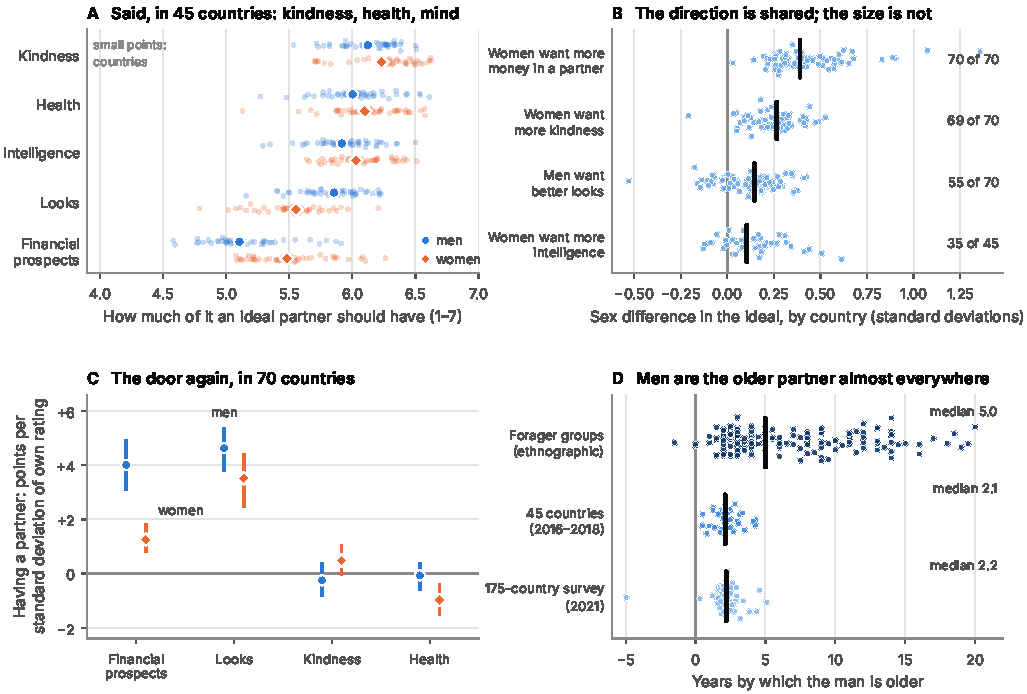
\includegraphics[width=\textwidth]{figures/fig8_world.pdf}
\caption{\textbf{The direction is shared; the size is cultural.} \textbf{(A)}~How much of each quality an ideal long-term
partner should have, in 45 countries (large markers: all respondents; small points: country means)~\cite{walter2020}.
\textbf{(B)}~Sex difference in the ideal, one point per country, in pooled standard deviations, signed so that the commonly
reported direction is positive; bar: median; right: countries with that direction. Intelligence from the 45-country
file~\cite{walter2020}, the rest from the 175-country file~\cite{kowal2025}. \textbf{(C)}~Change in the probability of having
a partner per standard deviation of a person's rating of their own financial prospects, looks, kindness and health, within
country and sex and holding age fixed, with 95\% intervals from resampling countries~\cite{kowal2025}. \textbf{(D)}~Years by
which the man is the older partner: \CcAgeN{} forager groups~\cite{binford2001} and country means from the two
surveys. Countries are units of replication and none is named. Source: authors' analysis of open data.}
\label{fig:world}
\end{figure*}

\emph{Stated ideals in 45 and 175 countries.} Two open cross-national files let the claim be checked. In 45 countries
(\WtN{} people~\cite{walter2020}) both sexes say an ideal partner should above all be kind (\WtKindM{} for men and
\WtKindW{} for women, of 7), healthy, and intelligent (\WtIntM, \WtIntW); looks (\WtLooksM, \WtLooksW) and financial
prospects (\WtResM, \WtResW) come below. Women rate intelligence above both looks and money in \WtIntAboveW{} of the 45
countries and men in \WtIntAboveM{} (Fig.~\ref{fig:world}A). A good mind is what people everywhere say they want, and it
is what four minutes cannot show them (Section~\ref{sec:resjury}). That gap between the wish and the evidence is the space
this hypothesis occupies. In the larger file (\WdPeople{} people in \WdCtry{} countries with at least fifty respondents of
each sex~\cite{kowal2025}) women want better financial prospects in a partner than men do in all \WdResPos{} countries, but
the difference runs from \WdResLo{} to \WdResHi{} standard deviations (median \WdResD). Men want better looks in
\WdLooksPos, by a median of only \WdLooksD, with reversals in the rest (Fig.~\ref{fig:world}B). Given thirty points to
divide among six qualities, both sexes give the most to kindness. Across countries the difference in wanting resources is
smaller where respondents hold more equal views of the sexes (rank correlation \WdEqRes; \WdEqResCI), as one earlier study
found and another did not~\cite{zentner2012,walter2020}, while the difference in wanting looks is larger there
(\WdEqLooks; \WdEqLooksCI). The man is the older partner on average in \WdAgePos{} of \WdAgeCtry{} countries and in all
\WtAgePos{} of the smaller sample, by a median of \WdAgeGap{} years against \CcGap{} among foragers
(Fig.~\ref{fig:world}D). These are convenience samples answering questionnaires, and countries are not independent of one
another.


\emph{Who assesses varies most.} Kin arrange most marriages among foragers~\cite{walker2011}. In the United States meeting
online is now the most common way for heterosexual couples to meet, and the part played by friends and family has
shrunk~\cite{rosenfeld2019}. By Proposition~\ref{prop:staging} that is a move from unstaged evidence held by people who
know the candidate to staged evidence exchanged between strangers. Cues of capacity survive the move; evidence of delivery
does not (prediction P28).

\emph{The floor moves with the marriage system and the sex ratio.} About 85\% of societies in the anthropological record
have permitted polygyny~\cite{henrich2012}, which raises the share of men left unpaired and, by
Corollary~\ref{cor:floor}, the intensity of selection on whatever wins wives there; normative monogamy shrinks the pool of
unmarried men~\cite{henrich2012}. Among eight Makushi communities men's mating effort resembled women's where men were in
surplus and turned toward short-term relationships only where men were scarce~\cite{schacht2015}.

\emph{What counts in a partner tracks what each sex contributes locally.} Men's greater weight on youth and looks, and
women's on resources, appear across 45 countries~\cite{walter2020}, but both sexes choose partners nearer their own age
where gender equality is greater~\cite{walter2020}, and the size of the preference gap fell with gender parity in one
analysis~\cite{zentner2012} and not robustly in another~\cite{walter2020}. Where a wife's earnings cross a norm the market
registers it: the share of couples in which the wife earns just over half of household income drops
sharply~\cite{bertrand2015}, and promotion to a top job doubled the probability of divorce for women and not for men, in
traditional couples only~\cite{folke2020}. Cues are local as well: heavier bodies were preferred in poorer
sites~\cite{swami2010}, masculine faces where health was worse~\cite{debruine2010}, and the usual readings of facial
masculinity were weak or reversed in small-scale societies~\cite{scott2014}. None of this is a difference between kinds of
people. Each is a response to who pays, who watches and what is scarce.

\begin{table*}[t]
\caption{What varies among societies, and the link it moves. Each row cites a comparative study; ``moves'' names the
parameter of the models in Section~\ref{sec:theory} that the practice changes. The rows are associations across or within
societies, not experiments, and none ranks a population.}
\label{tab:culture}
\scriptsize
\begin{tabularx}{\textwidth}{@{}P{0.13\textwidth}LP{0.25\textwidth}P{0.17\textwidth}@{}}
\toprule
What varies & Evidence & Link and parameter it moves & Consequence in the model\\
\midrule
Who chooses &
Parents or kin arrange marriages in about 85\% of 190 foraging societies~\cite{walker2011,apostolou2007} and weigh investment
and cooperation more than their children do~\cite{buunk2008}; in the United States meeting online has displaced friends and
family~\cite{rosenfeld2019}. &
Link 1, who assesses; unstaged observation $(1-d)n$ and so the validity for delivery $R_p$. &
Delivery is selected where the jury knows the candidate (Proposition~\ref{prop:staging}).\\
Marriage system &
About 85\% of societies have permitted polygyny~\cite{henrich2012}; polyandry is permitted in 53 societies outside its classical area, most often egalitarian
ones~\cite{starkweather2012}; beliefs in several fathers per child are widespread among 128 lowland South American
societies~\cite{walker2010}. &
Link 4, the episode; the share of men unpaired, $q$. &
Intensity $\varphi(z_q)/(1-q)$ rises with $q$ (Corollary~\ref{cor:floor}).\\
Payments and service &
Brideservice, brideprice or exchange in about 80\% of foraging societies~\cite{walker2011}; marriage payments of four to six
times annual household income, whose direction has switched within societies~\cite{anderson2007}. &
Enforced delivery $e$ before and at marriage; which family assesses. &
Capacity is selected before commitment (Proposition~\ref{prop:enforce}).\\
Sharing norms &
Meat widely shared, much of it on demand, with ridicule and exclusion for those who
refuse~\cite{woodburn1982,peterson1993,wiessner2005}. &
Enforced delivery $e$ to the band. &
As above; standing is conferred by those who receive.\\
Sex ratio &
Men's mating effort resembles women's where men are in surplus~\cite{schacht2015}; sociosexuality tracks sex ratio across 48
nations, with sex differences in every one~\cite{schmitt2005}. &
Which sex must be accepted; the floor $q$. &
The floor falls on the more numerous sex.\\
Women's earnings and gender equality &
Partners' ages converge with gender equality~\cite{walter2020}; a drop in couples where the wife out-earns the
husband~\cite{bertrand2015}; divorce after women's promotion~\cite{folke2020}; single women understating ambition before
single men~\cite{bursztyn2017}; wives now the more schooled spouse~\cite{esteve2016}. &
Link 5, aim: the weight on a woman's capacity $b$, and what she displays. &
Display follows the audience's weights; validity for women's capacity falls where it is penalized.\\
Health and subsistence &
Heavier bodies preferred in poorer sites~\cite{swami2010}; masculine faces preferred where health is
poorer~\cite{debruine2010}; standard readings of facial masculinity weak or reversed in small-scale
societies~\cite{scott2014}; Hadza and Shuar partners valued for work and character~\cite{marlowe2004,pillsworth2008}. &
Link 2, what is observed: which cues carry weight. &
Cue validity is local (Corollary~\ref{cor:cue}).\\
Paternal investment &
Jealousy is more severe where fathers invest more and extramarital sex is rarer, across 11
populations~\cite{scelza2020}; the romantic kiss is present in 46\% of 168 cultures~\cite{jankowiak2015}. &
Mean delivery $\bar p$ and how it is policed; the form of display. &
Capacity matters in proportion to $\bar p$ (Proposition~\ref{prop:delivery}).\\
Division of labor &
Tsimane adults command a broad common repertoire~\cite{schniter2015}; occupational specialization narrows comparison to one
domain. &
Link 5, aim: the number of common domains $K$. &
Generalist aim weakens by $Kc_K$ (Proposition~\ref{prop:division}).\\
\bottomrule
\end{tabularx}
\end{table*}

\subsection{The jury is being dismissed}\label{sec:resvillage}

\begin{figure*}[t]
\centering
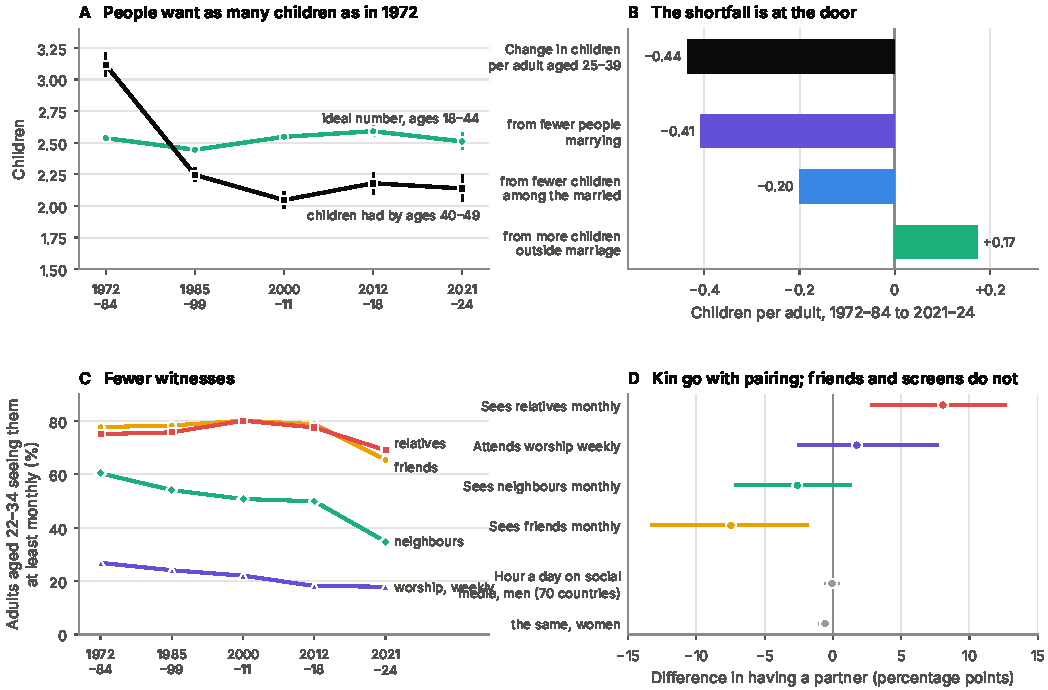
\includegraphics[width=\textwidth]{figures/fig9_village.pdf}
\caption{\textbf{Wanted, paired, born: the United States, 1972--2024.} \textbf{(A)}~Ideal number of children for a family
(adults aged 18--44) and number of children had (adults aged 40--49), by survey period, with 95\% intervals.
\textbf{(B)}~Change in children per adult aged 25--39 between 1972--1984 and 2021--2024, divided into the part due to more
people never marrying and the parts due to change within marital status. \textbf{(C)}~Adults aged 22--34 who spend a social
evening at least monthly with friends, relatives or neighbors, and who attend worship weekly. \textbf{(D)}~Difference in the
percentage with a steady partner between adults aged 22--34 who do and do not have each tie, holding age, sex, schooling,
income rank and survey year fixed; and, in grey, the difference per daily hour of social media in the 175-country
survey~\cite{kowal2025}. Associations, with 95\% bootstrap intervals. Source: authors' analysis of public
data~\cite{gss2024}.}
\label{fig:village}
\end{figure*}

If minds are read by juries over years, a society that dismisses the jury should find pairing harder. Three observations
from the United States fit that expectation, and three do not.

\emph{People want as many children as they did.} Asked the ideal number of children for a family, adults aged 18--44 said
\VgIdealOld{} in 1972--1984 and \VgIdealNew{} in 2021--2024, and those who had never married said \VgIdealNever{}
(Fig.~\ref{fig:village}A). The number people have had by their forties fell from \VgActOld{} to \VgActNew{} over the same
years. It stands at \VgActNever{} among the never married and \VgActEver{} among the ever married.

\emph{The shortfall is at the door.} Among adults aged 25--39 the number of children fell from \VgKidsOld{} to \VgKidsNew{}
per person, while the share never married rose from \VgNevOld\% to \VgNevNew\% (Fig.~\ref{fig:main}F). The move toward the
never married accounts for \VgMarr{} of the \VgChange{} (\VgMarrShare\%; \VgMarrShareCI). Change among the married
contributed \VgWithinEver, and more children outside marriage \VgWithinNever{} (Fig.~\ref{fig:village}B).
This is an accounting of where the births went and not a cause, since people who want no children may not marry. But the
stated ideals did not move. Later and less marriage runs with later and fewer births in East Asia too~\cite{raymo2015}, the
recent Nordic decline is of births forgone and not only postponed~\cite{hellstrand2021}, and no economic or policy change
since 2007 explains much of the American one~\cite{kearney2022}.

\emph{There are fewer witnesses.} Among adults aged 22--34, \VgNeighOld\% spent a social evening with a neighbor at least
monthly in 1972--1984 and \VgNeighNew\% in 2021--2024; with friends, \VgFriOld\% and \VgFriNew\%. Weekly worship fell from
\VgWorOld\% to \VgWorNew\%, and time online rose from \VgOnlineOld{} to \VgOnlineNew{} hours a week since 2000--2011
(Fig.~\ref{fig:village}C; the latest surveys were partly self-administered, which may affect these answers). The share with
no sexual partner in the past year rose from \VgNoPartOld\% to \VgNoPartNew\%, and among men from \VgNoPartMOld\% to
\VgNoPartMNew\%, as others report~\cite{ueda2020,twenge2017,lei2021}. Meeting online has displaced introduction by friends
and family as the commonest way for couples to form~\cite{rosenfeld2019}. In the terms of the model, a jury holding years
of unstaged evidence gives way to one observer holding a profile, which is all test (Proposition~\ref{prop:staging}). If a
commitment waits until a partner's delivery is known to a given reliability, the wait is inversely proportional to the
number of independent witnesses and to the unstaged share of what they saw (Proposition~\ref{prop:waiting}): \NtWaitCamp{}
periods for a camp of thirty, \NtWaitFive{} for five friends, \NtWaitOne{} for one observer alone. A fertile window is
finite, so a longer wait means fewer births.

\emph{What does not fit.} Young adults who see relatives at least monthly are more often partnered (\VgAsRel{} points;
\VgAsRelCI), but those who see friends monthly are less often partnered (\VgAsFri; \VgAsFriCI), and neighbors and worship
show nothing reliable (Fig.~\ref{fig:village}D). Kin are the jury of the ethnographic record, so the first result is the
one the theory expects; but single people have more evenings free, and one survey cannot order cause and effect. Across 70
countries an hour more a day on social media goes with \WdScrM{} points more singlehood among men (\WdScrMCI) and
\WdScrW{} among women, which is next to nothing. And in one national panel couples who met online married sooner, not
later~\cite{rosenfeld2017}. The claim that survives is narrow. Births are being lost before couples form, at the step where
evidence about a partner is thinnest and, for men, where selection on standing is strongest and rising
(Table~\ref{tab:funnel}). Specialization belongs in the same account. It lengthens training, which postpones first
births~\cite{nibhrolchain2012}. It moves people away from kin, and thinner kin networks are a leading explanation of the
transition to small families~\cite{newson2005,sear2011,colleran2020}. And it replaces common comparison on many domains with
separate ladders, the condition under which selection stops favoring the generalist (Proposition~\ref{prop:division}).
Whether generalists are the better adapted to survive is not something these data can show.

\subsection{Small brains, shrinking brains and restless minds}\label{sec:reshominins}

Neanderthals reached brain sizes like ours in communities far smaller than those of later
\Hs~\cite{prufer2014,skov2022}, so no account may depend on large networks. The present one does not: in a small community
everyone observes everyone for years, so validity can be high, while the number of candidates, and hence intensity, is
low. The prediction for such populations is a slower and noisier response, not none. The two lineages also differ in
organization more than in size: Neanderthal endocasts are elongated where ours became globular~\cite{neubauer2018}, so
volume is the wrong variable for comparing their cognition and the right one for the energetic argument, since tissue is
what costs. Small-brained species persisted while large-brained ones lived elsewhere, so no account may treat enlargement
as inevitable. \textit{H.~floresiensis} is the clearest case, and it meets the conditions under which the model expects
the least response: a small population isolated on an island~\cite{sutikna2016,brumm2016}, with few candidates to choose
among and a tight energy budget. \textit{H.~naledi} is harder, since large-brained people lived in Africa at the
time~\cite{dirks2017}. In the model, tissue follows demand only when it is functionally coupled to capacity and affordable
(Proposition~\ref{prop:tissue}); cheaper calories and shared care relax the second
condition~\cite{carmody2011,hawkes1998,burkart2014}. A model given the dates of such relaxations reproduces stasis and steps, but
that is a consistency check and not a test.

\emph{Smaller brains, more of the alleles.} Brain mass has fallen since the late Pleistocene, by more than 5\% in 50,000
years on one estimate and largely in step with body size~\cite{stibel2021,ruff1997}; whether it fell again in the last few
thousand years is disputed~\cite{desilva2021,villmoare2022}. Over the last ten thousand years in West Eurasia, meanwhile,
combinations of alleles that today predict measures of cognitive performance rose by about one standard deviation on the
scale of present variation~\cite{akbari2026}. The two are compatible. Selection through assessment acts on performance,
and performance can be had from more tissue or from better use of it. When tissue becomes dearer or its marginal return
falls, the response moves to the second route (Proposition~\ref{prop:tissue}). The pattern is selection for doing more
with less, which is what engineers obtain when a small model is trained to match a large one~\cite{hinton2015}. The
caution of the source applies: those alleles were scored in industrial societies, and what they did in a Neolithic
village is unknown.

\emph{Restless minds.} Variants of the dopamine receptor gene \textit{DRD4} that are associated with novelty seeking and
with attention-deficit diagnoses show signs of past positive selection~\cite{ding2002,williams2006} and are commoner in
populations that migrated farther~\cite{matthews2011}. Among Ariaal men in Kenya, carriers were better nourished than
non-carriers in a nomadic community and worse nourished in a settled one~\cite{eisenberg2008}. In a foraging task, adults
who screened positive for attention deficits left depleted patches sooner and earned more~\cite{barack2024}. The Ariaal
study gives no percentage advantage, and we could not trace the figure of 20\% sometimes quoted. Against a simple story of
lost advantage, alleles associated with the diagnosis have been declining in frequency since the Paleolithic, long before
farming~\cite{esteller2020}. The present framework adds one thing. A trait that helps in some domains and hurts in others
is neutral when people are compared on all of them, and it becomes a deficit in exact proportion to its mean loading on
whatever narrower set a test covers (Corollary~\ref{cor:narrow}; simulated slopes \NtNarBroad{} and \NtNarHurt). Years of
seated, sustained, solitary work are such a set. On this reading a diagnosis measures a variant against a test. It does
not show that the variant was built for the forest. For heightened smell or hearing as selected traits we found no
comparable evidence: foragers name odors far better than neighboring farmers who speak a closely related
language~\cite{majid2018}, which points to practice and not to genes.

\section{Discussion}

\subsection{What we conclude}\label{sec:conclude}

Asked as ``is intelligence attractive?'', the hypothesis has no clear answer: measured intelligence can be detected but is
not itself attractive~\cite{driebe2021}, and stated preferences predict choices weakly~\cite{todd2007,eastwick2014,eastwick2025}.
Asked link by link, it yields eight conclusions. Each is marked as measured here, derived, or conjectured.

\textbf{1. Minds are read by communities, not by suitors} (measured; derived). In 45 countries both sexes say they want
kindness and intelligence in a partner above looks and money. In four minutes neither can be read: strangers do not agree
on who has them, and choose on looks. Reading a mind dependably takes dozens of independent observers or years of
acquaintance, and shared gossip does not substitute for either.

\textbf{2. The chooser was a jury, and the bride was often not asked} (measured in the coded record). The hypothesis needs
long observation by whoever decides. It does not need romance or consent. Coercion subtracts from it in proportion to its
share and selects the body in its place.

\textbf{3. Breadth built generality} (derived). Comparing everyone on $K$ kinds of performance multiplies selection on
general ability $K$-fold relative to any specialty. Separate ladders remove the multiplier.

\textbf{4. A test shows capacity; only conduct shows delivery} (derived). Safe, repeated contests can replace dangerous
ones for the first and never for the second, which must be watched on unremarkable days or enforced by third parties.

\textbf{5. Men are selected at the door and women after it} (measured in the United States; the door also in 70
countries). The door is a floor on standing, and it has been rising for men in each cohort. Selection on women runs
through when and whether births follow.

\textbf{6. ``Half of all men never reproduced'' misreads a real asymmetry} (derived; measured). The genetic record gives a
ratio of effective numbers. It shows that men's reproduction was the more unequal, not how many men had none.

\textbf{7. Culture sets the weights, not the links} (measured in \CcSccsN{} societies and in 45 and 70 countries). Women
want resources in a partner more than men do in all \WdResPos{} countries of one survey and \WtResPos{} of 45 in the
other; the size of the difference varies forty-fold.

\textbf{8. The jury is being dismissed} (measured in one country; mechanism conjectured). Americans want the children they
wanted fifty years ago. Nearly all of the shortfall arises before a couple forms, while young adults see neighbors,
friends and congregations less and meet partners as strangers. A society that wants its births back might ask first how
people come to know each other well enough to commit.

On the brain itself the fossil record tests none of this. It leaves room for it, and smaller brains carrying more of the
alleles for performance is what selection on performance under a cost on tissue would produce (conjectured). Nine
selection drivers, four acting on men, four on women and one on both, are set out with their evidence in
Section~\ref{sec:hidden} (Table~\ref{tab:drivers}).

\subsection{What the evidence corrects}

Checked against the literature, eighteen common claims fare unevenly (Tables~\ref{tab:audit} and~\ref{tab:audittoday}). Restrained
fighting is the animal norm and not a human invention. Formal games are thousands of years old, not millions, and cannot
have caused a change that was complete long before. Body shape and facial symmetry are weak guides to fertility and
health~\cite{lidborg2025,pound2014}. Preferences do not shift toward masculine men across the cycle~\cite{wood2014,jones2018}. Of
masculine traits only strength predicts both mating and reproduction~\cite{lidborg2022}. More partners do not mean more
children. The part of the popular account that holds best is its widest: hunters, gatherers, makers, storytellers and
organizers were watched for a long time by people with a stake in judging them well.

\subsection{Is the mechanism still operating?}

In part, and not toward larger brains. The floor on men's access and the value of stable unions still operate. Marriage
gates less of reproduction than it did and selects more strongly on men's income. Timing operates with its sign reversed
for schooling. The drivers that acted through child survival contribute almost no variance where nearly all children
survive. The generalist aim has been narrowed by division of labor toward one occupation per person. Information about
ability is more abundant than ever, though nothing shows that it is used more accurately than a forager's years of direct
observation. The net effects are small beside environmental change: selection on education-linked variants is about 0.01
standard units per decade~\cite{kong2017}, test-score trends in both directions arise within
families~\cite{bratsberg2018}, and brain volumes rose across twentieth-century birth cohorts~\cite{decarli2024}. An
ancient-DNA study of 15,836 West Eurasians reports that combinations of alleles which today predict measures of cognitive
performance rose over the last ten millennia, with the caution that such effects were measured in industrialized societies
and their relation to what was adaptive in the past is unclear~\cite{akbari2026}; it does not show what was selected or
through which episode. For the foreseeable future, development, health, schooling and culture will move human cognition
far more than selection will.

\subsection{For builders of artificial minds}\label{sec:ai}

Nothing in the propositions is specific to genes. They describe any population of learners that is selected, or trained,
on a score, and nine of them bear on open problems in the evaluation of artificial systems. \emph{The score sets the aim,
not the pressure.} More intense selection on one score yields more of whatever the score loads on
(Proposition~\ref{prop:aim}); if reward is enough to produce intelligence~\cite{silver2021}, what is rewarded decides which
intelligence. \emph{Breadth selects generality.} Averaging over $K$ tasks that every candidate must attempt multiplies
selection on what the tasks share by $K$ (Eq.~\ref{eq:mainaim}), the formal case for ability-oriented over task-oriented
evaluation~\cite{hernandezorallo2017,legg2007}; a leaderboard on which each system is ranked on its best task restores the
specialist (Proposition~\ref{prop:division}), a single benchmark invites shortcuts~\cite{geirhos2020}, and aggregate scores
hide them~\cite{burnell2023}. \emph{Judges that share their errors agree without being right.} Independent evaluators add
accuracy as Eq.~\eqref{eq:sb} says; evaluators with a common source of error, such as one rubric or one body of training
data, add agreement and stop at the ceiling of Eq.~\eqref{eq:ceiling}, so agreement among judges does not measure their
accuracy. \emph{Breadth taxes gaming, except gaming that generalizes} (Corollary~\ref{cor:inflation}):
an indicator on which decisions depend comes under pressure~\cite{campbell1979}, and only evidence of a different kind
removes a general talent for passing tests. \emph{A recognized test measures capability, not disposition}
(Proposition~\ref{prop:staging}): an evaluation that a system can tell from use bounds what it can do and says nothing
about what it will do, so disposition has to be observed in use or made not to matter by limits on what the system can
reach (Proposition~\ref{prop:enforce}), the argument of a companion manuscript~\cite{taylor2026iina}. \emph{What is enforced
is no longer selected.} In the same proposition, guaranteeing an outcome removes the pressure that would have produced the
disposition to deliver it. \emph{A narrow test makes a deficit of a difference.} A system that trades strength on some
tasks for strength on others is neutral on a broad suite and fails a benchmark confined to its weak side
(Corollary~\ref{cor:narrow}); what a benchmark calls a defect may be a property of the benchmark. \emph{A price on size
selects efficiency.} Score selection with a cost on parameters moves gains from scale to use, as it appears to have done
in our own lineage and as distillation does by design~\cite{hinton2015}. \emph{A safe test can replace a dangerous one
only for capability} (Eq.~\ref{eq:ritual}): sandboxed trials, repeated, read what a system can do and say nothing of what
it will do when the stakes are real. These are parallels of form. They are not evidence about any system.

\subsection{Relation to other accounts}

The mechanism is an amplifier on the demand side. It does not replace ecological, social or cultural
accounts~\cite{kaplan2000,gonzalezforero2018,dunbar1998,muthukrishna2018}, which say why capacity is useful; it specifies a
channel through which usefulness could become persistent selection, and it makes predictions they do not: that breadth of
common comparison matters more than depth of culture, that the criterion of standing matters more than the intensity of
competition, that a preference cannot outrun the instrument that serves it, and that selection weakens where access is
decoupled from assessed performance. It does not explain the energy budget or the developmental supply of variants.

\subsection{Limitations}

No ancestral parameter is estimated. The models are Gaussian and mostly one-generation. Deception enters only in its
simplest form, delivery conditional on being assessed (Proposition~\ref{prop:staging}); display and assessment do not
coevolve, and enforcement is given, not derived. A product of correlations cannot show that the channel operated, and we
make no such claim (Section~\ref{sec:strength}). Phenotypic validity is not genetic accuracy. The generalist results assume
independent, equally weighted domains. The speed-dating sample is graduate students at one university, selected for
academic ability, in a setting that is all test; the law of Eq.~\eqref{eq:sb} should travel, the particular agreements
need not. The survey analysis is phenotypic and from one country, and its access component includes chosen childlessness
and infertility. The cross-cultural rows are associations. The ethnographic codes are outsiders' judgments of recently described societies, the cross-national files are convenience samples of self-report, and the division of falling births is an accounting and not a cause. Claims were checked against abstracts, not full texts. A
register of \NObj{} objections and the conditions under which the pathway fails are in Sections~\ref{sec:redteam}
and~\ref{sec:limits}.

\subsection{What would count against it}

Section~\ref{sec:predictions} lists \NPred{} predictions with the results that would weaken each. Seven are decisive.
Diverse observation should beat repeated observation of one domain at fixed total time (P2). Standing should track
independently measured general capacity where it is conferred as prestige and not where it is taken by force (P5, P13). In
natural-fertility populations selection on men's standing should lie in access at the low tail and not in family size among
fathers (P17). A person competent in several domains should be judged higher in general ability, and preferred as a
long-term partner or ally, over a specialist of equal total excellence (P22). Evidence of reliable investment should
raise the weight of competence in consequential choices (P23). Judgments of reliability formed from unannounced
observation should predict later conduct better than judgments formed from the same amount of staged interaction, with the
reverse for ability (P24). And lengthening an encounter or adding observers should shift the weight of choice toward
intelligence and sincerity (P27). If these fail, the mechanism fails with them.

\section{Methods}\label{sec:methods}

\emph{Fossil record.} Three open compilations were used as published: 233 crania with consensus dates and
volumes~\cite{gingerich2022}, 166 \Homo{} specimens with taxon, age and site~\cite{will2021}, and 94 early
hominins~\cite{du2018}. Piecewise-linear models of log volume on time were compared by AICc and BIC; change points were
located by grid search with \FosBoot{} bootstrap resamples. Regional series were assigned by site coordinates
(Section~\ref{sec:explananda}).

\emph{Theory and simulation.} The nineteen propositions are derived for Gaussian traits under additive inheritance
(Section~\ref{sec:theory}); proofs are in Section~\ref{app:proofs}. Each was checked by Monte Carlo or individual-based
simulation against its exact value, and re-derived by an independent construction that shares no code with the experiments
(Section~\ref{sec:experiments}). Parameter values are illustrations, not estimates.

\emph{Speed dating.} The public file of the Columbia experiment~\cite{fisman2006} has \SdRows{} rows, one per person per
meeting, for \SdN{} people. Ratings are on a 1--10 scale and were
centered on each rater's mean. Agreement between two observers is the one-way intraclass correlation among the ratings a
person received; agreement between panels is the correlation, across persons, of the means of two disjoint random sets of
$k$ raters. What predicted a yes is a linear probability model of the decision on the six ratings,
standardized over all meetings, with a fixed effect for each chooser, fitted separately by sex, using either the chooser's
own ratings or the mean rating the partner received from everyone else. Expected interest is the 1--10 guess that the
partner would say yes, rescaled to 0--1. Intervals are percentile bootstraps over persons. Variables describing race and
religion were not used (Section~\ref{sec:speed}).

\emph{Present-day selection.} The General Social Survey cumulative file, 1972--2024~\cite{gss2024}, supplied \GssN{} respondents
aged 45--79 born 1900--1979 with known number of children. Traits were years of schooling, a ten-word vocabulary test,
occupational prestige, and the logarithm of personal income at ages 45--64. Each trait was standardized, and fitness made
relative, within sex and decade of birth; cells were combined by their weights. Access, number, pairing and conversion
follow Eq.~\eqref{eq:split}. Survey weights were applied. Intervals are percentile bootstraps (\GssBoot{} resamples of
respondents within cells; 500 to 1,000 for the later analyses). Results were stable without weights, in the age window
50--74, and in surveys before and after 1990 (Section~\ref{sec:sitables}). Only aggregates by sex and cohort are reported.

\emph{Ethnographic codes.} We used the D-PLACE release~\cite{kirby2016} of the Standard Cross-Cultural
Sample~\cite{murdock1969} (\CcSccsN{} societies), of the Ethnographic Atlas (\CcEaN) and of Binford's hunter-gatherer
compilation~\cite{binford2001} (\CcBinN{} groups): who chooses a spouse, and wife-beating~\cite{broude1983};
consent~\cite{frayser1985}; rape~\cite{broude1976,sanday1981book}; captives~\cite{white1988}; divorce~\cite{whyte1978}; ages at
first marriage and polygyny~\cite{binford2001}; games~\cite{roberts1959}. Foragers are societies whose dominant subsistence is
gathering, hunting or fishing. Missing codes were dropped variable by variable. Societies share ancestry and neighbors, so
we give counts and shares and claim no significance across them; the interval for the forager age gap resamples groups and
ignores their relatedness. For games we report presence only (Section~\ref{sec:notes}).

\emph{Cross-national surveys.} The 175-country file~\cite{kowal2025} (\WdN{} rows) and the 45-country
file~\cite{walter2020} (\WtN{} rows) were read as deposited. A country enters a country-level analysis if it has at least
fifty men and fifty women with the variable (thirty in the smaller file). Sex differences are differences in pooled
standard deviations. Having a partner was regressed on four self-ratings standardized within country and sex, with age and
its square, after removing country means; intervals resample countries. No country is named or ranked.

\emph{Births, ideals and ties.} A second extract of the General Social Survey supplied marital status, number of
children, ideal number of children, social evenings, worship, hours online and partners in the past year. The change in
children per adult aged 25--39 was divided, by the standard decomposition of a difference between two rates, into a part
due to the share never married and parts due to change within marital status. Effective numbers use
$N_e/N=\bar k/(\bar k-1+V/\bar k)$ on completed families, which equals Eq.~\eqref{eq:ancestors} identically. Ties were
related to having a steady partner by a linear probability model with age, sex, schooling, income rank and year.

\emph{Literature.} Searches ran to November 10, 2026. Of \RefCited{} references, \RefResolved{} have a DOI resolved
against Crossref; specific claims were checked against abstracts where one could be retrieved, and otherwise limited to
what the title states.

\section*{Data and code availability}

\noindent All code, results and the three fossil datasets are in the accompanying package; one script rebuilds every number,
table and figure. The survey file and the speed-dating file are public and are downloaded by scripts that verify them, not
redistributed (Section~\ref{app:repro}).

\section*{Acknowledgments and AI-assistance disclosure}

\noindent Jepson Taylor conceived the hypothesis and directed the work: that reciprocal assessment of intelligence, drive
and condition through hunting, contests, play and games, before lifetime outcomes are known, could have accelerated
selection on human cognition; that selection favored generalists over specialists; and the account examined in
Section~\ref{sec:audit}. Section~\ref{sec:verification} was prompted by a companion manuscript on the oversight of artificial
agents~\cite{taylor2026iina}. The authors' review of the previous version raised the ten questions answered in
Section~\ref{sec:notes}, which led to Sections~\ref{sec:reschoice} and~\ref{sec:resvillage}, to
Propositions~\ref{prop:ancestors} and~\ref{prop:waiting}, and to the passages on ritual contests, shrinking brains and
restless minds; each author's contribution is to be confirmed before submission. Literature search and synthesis, mathematics, code, simulations, data analysis, figures and drafting
were carried out with Claude (Anthropic); earlier drafts also used ChatGPT (OpenAI). The main graphic and all figures are
generated by code from the results and data; no figure was produced by an image-generation model. The manuscript has not
been externally reviewed. A human author must verify the claims, settle authorship and affiliation, and take responsibility
for the content before any submission; journals differ in their policies on AI-assisted manuscripts, and those policies
should be checked for the chosen venue.


\clearpage
\twocolumn[{\noindent{\sffamily\scriptsize\color{accent}\textbf{SUPPLEMENTARY INFORMATION}}\par\vspace{4pt}
\noindent{\sffamily\bfseries\fontsize{17}{20}\selectfont Performance {\color{accent}Before Outcomes}\par}\vspace{3pt}
\noindent{\sffamily\fontsize{10.5}{13}\selectfont\color{ink2} It takes a village to read a mind: how being judged at everything, by people who knew us for years, could build a mind for anything, and what happens when the jury goes home\par}\vspace{4pt}
\noindent{\color{rulegray}\rule{\textwidth}{0.5pt}}\par\vspace{4pt}
\noindent{\small Contents: S1~scope and claim levels; S2~the fossil record; S3~ten claims about ancestral selection, checked; S4~evidence base;
S5~theory; S6~numerical experiments; S7~mate selection today, with a speed-dating experiment; S8~ten questions raised in review, answered; S9~nine drivers; S10~is the
mechanism still operating; S11~how strong must selection be; S12~other hominins; S13~predictions and a first study; S14~limitations; S15~objections;
S16~the oldest games; S17~additional tables; S18~proofs; S19~reproducibility and data.\par}\vspace{10pt}}]
\setcounter{section}{0}\renewcommand{\thesection}{S\arabic{section}}\renewcommand{\theHsection}{S\arabic{section}}
\setcounter{figure}{0}\renewcommand{\thefigure}{S\arabic{figure}}\renewcommand{\theHfigure}{S\arabic{figure}}
\setcounter{table}{0}\renewcommand{\thetable}{S\arabic{table}}\renewcommand{\theHtable}{S\arabic{table}}
\setcounter{equation}{0}\renewcommand{\theequation}{S\arabic{equation}}\renewcommand{\theHequation}{S\arabic{equation}}
\section{Scope, claim levels and verification}\label{sec:scope}

\noindent Every statement in the paper belongs to one of the levels in Table~\ref{tab:levels}, and tables and figures name the
level of what they report. The main text states results; this Supplementary Information gives the audit of the fossil rate
(Section~\ref{sec:explananda}), the evidence base (Sections~\ref{sec:audit},~\ref{sec:evidence} and~\ref{sec:today}), the theory
with proofs (Sections~\ref{sec:theory} and~\ref{app:proofs}), the numerical experiments (Section~\ref{sec:experiments}), the
evidence for each driver (Section~\ref{sec:hidden}), the predictions and a first study design (Section~\ref{sec:predictions}),
the limitations (Section~\ref{sec:limits}), a register of objections (Section~\ref{sec:redteam}) and what is needed to rebuild
every number (Section~\ref{app:repro}).

\begin{table}[t]
\caption{Claim levels used throughout.}\label{tab:levels}
\footnotesize
\begin{tabularx}{\columnwidth}{@{}P{0.27\columnwidth}L@{}}
\toprule
Level & Meaning and permissible inference\\
\midrule
External evidence & A cited observation or result, restricted to its population and design.\\
Reanalysis & A computation on published open data, reproducible from the package.\\
Exact result & A consequence of stated assumptions; not a measurement of history.\\
Numerical check & An executed simulation verifying an implementation or probing sensitivity.\\
Plausibility bound & An order-of-magnitude comparison combining published summaries with stated assumptions.\\
Testable hypothesis & A relationship new observations could support or reject.\\
Historical conjecture & An unverified claim about ancestral timing, magnitude, or anatomy.\\
\bottomrule
\end{tabularx}
\end{table}

\section{What needs explaining: rate, pattern, parallels}\label{sec:explananda}

\subsection{The per-generation rate}

\noindent ``Rapid'' needs a denominator. Three quantities are often run together: net change per year in the fossil record,
inherited response per generation, and the part of that response attributable to a proposed mechanism. A large endpoint
difference establishes neither of the last two. Gingerich's consensus series regresses log endocranial volume (ECV) on time
with slope 0.416 per million years over about 3.19~million years, uses a within-population standard deviation of 0.10 for
$\ln$~ECV, and assumes a 25-year generation~\cite{gingerich2022}. The implied total change is \RateTotalSD{} within-population
standard deviations over about \RateGens{} generations, or $\RateBase$ haldanes (standard deviations per generation).
Table~\ref{tab:rates} varies the generation time and the fraction of the interval in which change occurred. Even if all change
were packed into a tenth of the time, the required rate stays near $10^{-3}$ haldanes. For comparison, the median absolute
linear selection gradient in natural populations is 0.16~\cite{kingsolver2001}. Du and colleagues likewise found that
within-lineage brain size evolved far more slowly than traits change in living populations~\cite{du2018}.

\textit{Reanalysis.} We refitted the series from the published specimen data (Supplementary Dataset~1
of~\cite{gingerich2022}; $n=\FosN$). Ordinary least squares of $\ln$~ECV on age gives a slope of $\FosSlopeSpec\pm\FosSlopeSpecSE$
per Myr at the specimen level and $\FosSlopeBin\pm\FosSlopeBinSE$ across the \FosBins{} occupied 100-kyr bins, bracketing the
published value. The pooled within-bin standard deviation is \FosSDw, a little above the 0.10 used in the original. Across
these choices the long-run rate is $(\FosRateLo$--$\FosRateHi)\times10^{-4}$ haldanes. The rate audit does not depend on one
summary.

\begin{table}[t]
\caption{Required long-run rate (haldanes) for the hominin ECV increase.}\label{tab:rates}
\footnotesize
\begin{tabularx}{\columnwidth}{@{}Xcccc@{}}
\toprule
 & \multicolumn{4}{c}{Fraction of interval with directional change}\\
\cmidrule(l){2-5}
Generation (yr) & 1.0 & 0.5 & 0.25 & 0.1\\
\midrule
\tabinput{generated/tab_rates.tex}
\bottomrule
\end{tabularx}
\tablenote{Inputs: slope 0.416 $\ln$~ECV per Myr and $s=0.10$~\cite{gingerich2022}. Using $s=0.08$ raises each entry by 25\%.
Claim level: plausibility bound.}
\end{table}

\subsection{Is selection needed at all?}

If the rate is so small, could drift alone have produced it? Lande's benchmark gives the variance of neutral change in the
mean after $t$ generations as $h^2t/N_e$ in phenotypic variance units~\cite{lande1976}. Table~\ref{tab:drift} reports the
standardized departure $z$ of the observed \RateTotalSD{} standard deviations from that expectation. With $h^2=0.5$, drift is
rejected for long-term $N_e\ge5{,}000$ but not for $N_e\approx1{,}000$. A mutational-input benchmark, which ignores all
constraint, is more permissive still: with mutational variance $10^{-3}V_E$ per generation~\cite{lynch1990} the departure is
only $z=\MutZLo$--$\MutZHi$.

\begin{table}[t]
\caption{Departure ($z$) of the observed change from Lande's neutral benchmark.}\label{tab:drift}
\footnotesize
\begin{tabularx}{\columnwidth}{@{}Xccccc@{}}
\toprule
 & \multicolumn{5}{c}{Long-term effective size $N_e$}\\
\cmidrule(l){2-6}
$h^2$ & 1,000 & 2,000 & 5,000 & 10,000 & 20,000\\
\midrule
\tabinput{generated/tab_drift.tex}
\bottomrule
\end{tabularx}
\tablenote{$z=\RateTotalSD/\sqrt{h^2t/N_e}$ with $t=\RateGens$ generations. Values $z<2$ mean drift cannot be excluded by
magnitude alone.}
\end{table}

Magnitude alone therefore cannot exclude drift under every defensible parameter set. Three considerations nonetheless weigh
against neutrality. First, cost: an organ that claims a large share of a child's energy budget~\cite{kuzawa2014} sits under
strong stabilizing selection, so a sustained shift in its mean implies a shift in the balance of costs and benefits, not
neutral wandering. Second, parallelism: several regional series rose together (Section~\ref{sec:parallel}), and drift has no
preferred direction. Third, the long-run increase arises mainly within species~\cite{puschel2024,du2018}.

\subsection{The pattern is stepwise, not a constant trend}

At 100-kyr resolution, Gingerich identifies four phases alternating between stasis and directional change, with boundaries
near 2.0, 1.5, and 0.7~Ma~\cite{gingerich2022}. Hubbe and Harvati fitted six evolutionary models to neurocranial and facial
landmark data for eight time-ordered groups in the \Hs{} and Neanderthal lineages; for the neurocranium, unbiased random walk
and stasis were best supported, and gradual directional selection played a limited role~\cite{hubbe2026}. This is a serious
challenge to any account that assumes a constant directional push. It is also typical of fossil series: directional change
is the best-supported model in only about 5\% of fossil sequences~\cite{hunt2007}, and stabilizing selection around a moving
optimum produces random-walk and stasis signatures at long timescales~\cite{estes2007}. Such fits describe the pattern at
the sampled resolution, not the process. A complete account needs a mechanism in which net selection keeps its sign while
realized change is gated by constraints.

\textit{Reanalysis.} The specimen data support the stepwise description but not its dates (Fig.~\ref{fig:fossils}A). A
constant trend is rejected against every piecewise alternative ($\Delta$AICc $=\FosAICLin$ and $\Delta$BIC $=\FosBICLin$ relative
to the best model under each criterion). A four-phase model with zero slope in phases~I and~III and free breakpoints lies
within $\Delta$AICc $=\FosAICStep$ of an unconstrained three-breakpoint model and is preferred to it by BIC. Its breakpoints,
\FosBpA, \FosBpB{} and \FosBpC~Ma, are close to the published ones, with levels of \FosLevI{} and \FosLevIII\ccm{} in the two
stasis phases (Table~\ref{tab:phases}). Two cautions follow. The unconstrained model puts small positive slopes in the
``stasis'' phases (\FosFreeSlA{} and \FosFreeSlC{} per Myr, against \FosFreeSlB{} and \FosFreeSlD{} in the directional phases),
and with \FosStIN{} and \FosStIIIN{} specimens those phases cannot exclude slow change (slopes $\FosStI\pm\FosStISE$ and
$\FosStIII\pm\FosStIIISE$). And the steps are poorly dated: bootstrap 95\% intervals for the three breakpoints are \FosCIA,
\FosCIB{} and \FosCIC~Ma. Stasis and steps is the better description; any test that relies on the exact timing of a step
is weak.

\begin{table}[t]
\caption{Phases of hominin brain-size change. Published phases are from the binned consensus series~\cite{gingerich2022}; fitted
values are from the stasis--step model applied here to the same \FosN{} specimens.}\label{tab:phases}
\footnotesize
\begin{tabularx}{\columnwidth}{@{}lllL@{}}
\toprule
Phase & Published (Ma) & Fitted (Ma) & Fitted level or rate\\
\midrule
I, stasis & 3.2--2.0 & 3.2--\FosBpA & \FosLevI\ccm\\
II, increase & 2.0--1.5 & \FosBpA--\FosBpB & \FosSlII{} per Myr; $\FosRateII\times10^{-4}$ haldanes\\
III, stasis & 1.5--0.7 & \FosBpB--\FosBpC & \FosLevIII\ccm\\
IV, increase & 0.7--0.01 & \FosBpC--0.01 & \FosSlIV{} per Myr; $\FosRateIV\times10^{-4}$ haldanes; ends at \FosLevEnd\ccm\\
\bottomrule
\end{tabularx}
\tablenote{Bootstrap 95\% intervals for the breakpoints (\FosBoot{} resamples): \FosCIA, \FosCIB, \FosCIC~Ma. Claim level:
reanalysis.}
\end{table}

The budget-limited mechanism developed in Section~\ref{sec:theory} predicts that directional phases begin after relaxations
of the energetic budget or of the information ceiling, with short lags. The record offers only weak tests. The onset of
phase~IV lies close to the earliest well-dated evidence for cooking, fish cooked at Gesher Benot Ya'aqov about 780,000 years
ago~\cite{zohar2022}, and follows fire at Wonderwerk Cave about one million years ago~\cite{berna2012}. Phase~II has no
comparably dated energetic marker. First appearances are lower bounds, the breakpoints carry intervals several hundred
thousand years wide, and dates should not be moved to fit episodes; the alignment is hypothesis-generating only.
Environmental variables also predict body and brain size in \Homo~\cite{will2021}, an alternative that any test must
include.

\subsection{Parallel series, and exceptions}\label{sec:parallel}

Large brains did not arise once. In the compilation of Will and colleagues~\cite{will2021}, log volume rises with time in three regional series over the
last 0.9~Myr (Fig.~\ref{fig:fossils}B): by \SerAfr{} per Myr (95\% bootstrap interval \SerAfrCI; $n=\SerAfrN$) from African Middle
Pleistocene \Homo{} to Pleistocene \Hs, by \SerEur{} (\SerEurCI; $n=\SerEurN$) from western Eurasian Middle Pleistocene \Homo{} to
Neanderthals, and by \SerAsia{} (\SerAsiaCI; $n=\SerAsiaN$) among East and Southeast Asian archaic \Homo, a series that includes
late-surviving \textit{H.~erectus}. These are regional series, not clean lineages, and gene flow connected
them~\cite{green2010,prufer2014}; but three rises are harder to attribute to chance than one. Neanderthals averaged
\NeaMean\ccm{} (SD~\NeaSD; $n=\NeaN$) and Pleistocene \Hs{} \SapMean\ccm{} (SD~\SapSD; $n=\SapN$): a difference of \WelchPct\%
(Welch $p=\WelchP$) that is half a within-group standard deviation and depends on which specimens a compilation includes.
Outside this compilation, the Harbin cranium, now attributed to Denisovans, has a volume near 1,420\ccm~\cite{ni2021,fu2025},
and one of the Xuchang crania is estimated near 1,800\ccm~\cite{li2017}.

Nor was enlargement universal. \textit{H.~naledi}, with the stature and body mass of a small modern human, had an endocranial
volume of 465--560\ccm{} and lived between 335 and 236 thousand years ago~\cite{berger2015,dirks2017}. \textit{H.~floresiensis}
had 426\ccm{} and is known from deposits 100 to 60 thousand years old~\cite{brown2004,kubo2013,sutikna2016}. A demand-side account must
leave room for lineages in which demand, if present, did not become tissue.

\subsection{The last 300,000 years}

Within Pleistocene \Hs{} there is no trend: means are \SapOld\ccm{} before 100~ka ($n=\SapOldN$), \SapMid\ccm{} for
100--30~ka ($n=\SapMidN$) and \SapLate\ccm{} for 30--10~ka ($n=\SapLateN$), in line with a reanalysis that found stability over
the last 300,000 years~\cite{villmoare2022}. Recent populations average about 1,349\ccm~\cite{beals1984}, \RecentDrop\% below the
terminal Pleistocene mean. That a reduction occurred is widely accepted; its timing is not. Proposals range from a gradual
Holocene decline that tracks a fall of about 10\% in body mass~\cite{ruff1997} to an abrupt drop about 3,000 years
ago~\cite{desilva2021,desilva2023}, which a reassessment of the same data did not find~\cite{villmoare2022}.
Section~\ref{sec:present} returns to what this means for the mechanism.

\subsection{The restated explananda}

A satisfactory demand-side account should address:
\begin{description}[leftmargin=2.1em,labelwidth=1.6em,labelsep=0.5em,itemsep=0.5pt,font=\sffamily\bfseries\footnotesize]
\item[Q1] \emph{Persistence}: why the net direction of change was sustained across some $10^{5}$ generations, through whatever
reversals occurred within them, instead of settling at an ecological optimum.
\item[Q2] \emph{Cost-paying}: why benefits kept pace as the organ grew more expensive.
\item[Q3] \emph{Parallelism with exceptions}: why several late lineages enlarged together while others stayed small.
\item[Q4] \emph{Pattern}: why stasis alternated with steps.
\item[Q5] \emph{Target}: why selection favored domain-general capacity rather than many separate specialized skills.
\item[Q6] \emph{Both-sex expression}: cognitive capacities differ little between the sexes. This is not diagnostic of mutual
choice, because shared autosomal inheritance transmits selection on either sex to both~\cite{lande1980}.
\item[Q7] \emph{Display surplus}: why humans invest heavily in costly, public, skill-revealing behavior with no immediate
subsistence return.
\item[Q8] \emph{Variance}: why substantial heritable variation in cognition persists.
\end{description}

\section{Ten common claims about ancestral selection, checked}\label{sec:audit}

\noindent A familiar account of how mating shaped the human mind runs as follows. As groups grew, subordinate males became
worth keeping as fighters; men learned to best one another without lasting harm; watching them wrestle, hunt and play revealed
health, drive and intelligence early in life; women and their families chose accordingly; and because the criteria came
before, not after, a lifetime's outcomes, the mind evolved faster. Women in turn were chosen on cues of fertility and health.
Versions of this account circulate widely, and it motivated the present work. It is easy to believe and hard to test, so
each claim is stated and checked in Table~\ref{tab:audit}. Three conclusions shape the rest of the paper.

\textbf{What survives.} The strongest part is the part about hunters (claim N8). Foraging skill is valuable, slow to
mature, variable among men, and hard to rank from a few observations; people in foraging societies say they care about
intelligence, persistence and hard work in a spouse; and better hunters have more children. That is the setting in which
early, repeated, public information should matter most. The claim about subordinate males as fighters (N1) also survives, and
Proposition~\ref{prop:despot} gives it a precise form.

\textbf{What is wrong.} Four things. Restrained fighting is not a human invention and does not require intelligence
(N2): it is the rule among animals. Contests of force select formidability, and comparative data give no sign that stronger
male contest enlarges brains (N3). Formal games are a few thousand years old and cannot have caused a change that was
complete hundreds of thousands of years earlier (N7; Section~\ref{sec:games}). And the cues by which men are said to choose
women (N9, N10) have weak validity as measured and aim largely at a life stage, which is not heritable.

\textbf{What changes in the theory.} The account treats public contest as a single thing that both intensifies
competition and reveals quality. The audit separates four quantities that the theory keeps apart: how accurately a
performance reveals a trait, how strongly standing governs reproduction, which trait the performance reveals, and whether the
performance can be repeated. Leveling within groups lowers the second; safe, varied performance raises the first and the
fourth; and the shift from dominance by force to standing by skill across many domains changes the third. The last of these,
not any increase in competition, is what points selection at a general-purpose brain.

\begin{table*}[t]
\caption{Ten common claims about ancestral selection, checked. Each is stated in the strong form in which it circulates.}
\label{tab:audit}
\scriptsize
\begin{tabularx}{\textwidth}{@{}P{0.022\textwidth}P{0.165\textwidth}P{0.085\textwidth}LP{0.20\textwidth}@{}}
\toprule
 & Claim & Verdict & Evidence and correction & Consequence for the theory\\
\midrule
N1 & As groups grew, subordinate males became valuable as extra fighters, so killing or maiming every rival became costly. &
Supported, restated &
Chimpanzees enter intergroup contests when they outnumber rivals, and killers outnumber victims by a median of eight to
one~\cite{wilson2002,wilson2014}; raids approximate Lanchester's square law~\cite{johnson2015}. Human male reproductive skew is low
for a mammal, in part because men cooperate~\cite{ross2023}, and foragers actively level would-be
dominants~\cite{boehm1993,boehm1999,gavrilets2012}. Corrections: what makes subordinates valuable is the strength of rival coalitions,
not the size of one's own group; ``alpha'' and ``beta'' misdescribe human status, which has a dominance route and a prestige
route~\cite{henrich2001,cheng2013}; and the antiquity and frequency of war are disputed~\cite{bowles2009,fry2013,gomez2016,lahr2016,sala2015}. &
Proposition~\ref{prop:despot}. Leveling lowers intensity (Proposition~\ref{prop:identity}), so by itself it slows selection; its
importance is what it does to the aim.\\
\addlinespace
N2 & Besting rivals without lasting harm became important; boxing or wrestling takes far more intelligence than two rams
butting horns. & Half right &
Restrained, ritualized contest is the animal norm and needs little
cognition~\cite{maynardsmith1973,parker1974,enquist1983,arnott2009}; the rams already do it. What is distinctive in humans: weapons
and coalitions make unregulated fights deadly for either party~\cite{wrangham2018,gintis2015}; contests are rule-bound, refereed,
watched and discussed; and they come in many kinds. Coalitional play fighting is recorded in all 46 forager culture clusters
with adequate descriptions~\cite{scalise2018}, and combat sports are almost exclusively male across 50
societies~\cite{deaner2013}. &
Proposition~\ref{prop:repeat}: a safe contest can be repeated, and repetition is information. The gain is accuracy, not
cleverness in the fighting itself.\\
\addlinespace
N3 & Watching men fight or wrestle revealed health, drive and intelligence, and became an early criterion in mating. &
Strength yes; intelligence weakly &
Observers judge strength and fighting ability accurately from bodies and faces~\cite{sell2009}; Sereer wrestlers have more
children~\cite{llaurens2009}; in one well-studied sample men's dominance, not their attractiveness to women, predicted mating
success~\cite{hill2013}, and contest may have been the main mode of sexual selection in men~\cite{puts2010}. Bystanders use
contests in mate choice in other species, though not always in favor of winners~\cite{doutrelant2000,ophir2003}. But across
primates, stronger male contest goes with body and canine dimorphism~\cite{plavcan2012} and with smaller relative
brains~\cite{schillaci2006}; across mammals it does not enlarge them~\cite{lemaitre2009,fitzpatrick2012}. &
Proposition~\ref{prop:aim}: a contest of force selects formidability. It bears on capacity only through its small loading on
skill.\\
\addlinespace
N4 & Because these were criteria applied before, not at the end of, life, the evolution of mind accelerated. &
Core idea, reworded &
Selection never waits for the end of life. What matters is how accurately those making consequential decisions (marriage,
alliance, support) can forecast a candidate's eventual value at the time they decide. Earlier information raises that
accuracy; in dairy cattle the same move raised genetic gain by 50--100\%~\cite{garciaruiz2016}. ``Accelerated'' needs care:
per generation the change was slow (Section~\ref{sec:explananda}). & Proposition~\ref{prop:identity}.\\
\addlinespace
N5 & Humans selected hero warriors: risk-takers with purpose, strength, and the intelligence to rally others. & Mixed &
Killers had more wives and children among Yanomam\"o~\cite{chagnon1988}, as did prolific raiders among Nyangatom elders, through
bridewealth~\cite{glowacki2015}; but the more aggressive Waorani warriors left fewer descendants~\cite{beckerman2009}. Societies
that offer warriors more rewards lose more men to war~\cite{glowacki2013}. Heroic, not gratuitous, risk is attractive in a
mate~\cite{farthing2005}. Theory predicts that
high-ranking men contribute most to between-group contests~\cite{gavrilets2014}. &
Courage in defense is one performance venue, and standing is how a group pays for a public good. Sign and size depend on
context.\\
\addlinespace
N6 & Women selected tribal leaders for power. & Partly &
Men's status predicts reproductive success across 33 nonindustrial populations~\cite{vonrueden2016}, and women weigh status
more than men do~\cite{buss1989,walter2020}. But forager leaders have little coercive power~\cite{boehm1999}; kin arrange most
forager marriages~\cite{walker2011,apostolou2007}; leaders in the ethnographic record are marked more by expertise and ``neural
capital'' than by dominance~\cite{garfield2019}; and among Tsimane both prestige and dominance pay, prestige chiefly through
wives who begin reproducing earlier~\cite{vonrueden2011}. Reproductive monopoly by powerful men is a Holocene
pattern~\cite{karmin2015,zeng2018} that enlarged no brains. &
The standing route ($\beta_S$), with assessors who are mostly kin. Power detached from assessed capacity is the decoupling
case (prediction~P8).\\
\addlinespace
N7 & Early games displayed the best players in public. & Too recent to be a cause &
Every attested formal game is younger than about 8,000 years, and all secure ones are younger than about 5,500
(Table~\ref{tab:games}): the last 0.2\% of the record, long after brains reached modern size. Games show the propensity. Play,
contest and coalitional play fighting, which are widely documented~\cite{roberts1959,deaner2013,scalise2018,pellis2000}, are the
ancestral analogue. & The mechanism needs public, repeated, outcome-revealing performance, not boards or stadia.\\
\addlinespace
N8 & Successful hunters needed determination, intelligence and health, and both sexes had early indicators of them. &
Supported; the strongest part &
Hunting skill peaks near age~33 and takes ten to twenty years beyond adult size to mature~\cite{koster2020,gurven2006}; better
hunters have more children~\cite{smith2004}. Hadza name ``intelligence'' and ``heart'' beside strong arms as what makes a
hunter~\cite{apicella2014}; Hadza women value intelligence and foraging in a husband, and men value hard work in a
wife~\cite{marlowe2004}. Yet reputations track measured skill only noisily~\cite{stibbardhawkes2018}, and daily returns vary too much
that large samples are needed to tell hunters apart by skill~\cite{hillkintigh2009}. &
The setting of the model: valuable, slow to reveal, noisy. Repetition, diversity and years of observation make it assessable
(Propositions~\ref{prop:portfolio} and~\ref{prop:repeat}; Table~\ref{tab:indicators}).\\
\addlinespace
N9 & Women were chosen for signs that they could bear many children: large hips, large breasts, good health. &
Largely unsupported as stated &
Men's preferences track youth and nubility~\cite{kenrick1992,lassek2019,marlowe1998}. The low waist--hip ratios and body-mass
indices judged most attractive, long read as signs of fecundity~\cite{singh1993}, do not indicate higher fertility or better
health~\cite{lassek2018a,lassek2018b,bovet2019}. A systematic review of direct fertility measures (19 articles, 68 effect
sizes) concluded that the evidence is too weak to support the claim that feminine morphology indicates reproductive potential:
a less feminine waist--hip ratio may reflect past births, and no study has related fertility to facial
femininity~\cite{lidborg2025}. One study
links larger breasts and narrow waists to higher estradiol~\cite{jasienska2004}. Where hips and fat do bear on brains is energy
and obstetrics: infant fat buffers the brain's fuel supply~\cite{kuzawa1998,cunnane2003}, gluteofemoral stores may supply
neurodevelopmental lipids~\cite{lassek2008}, and pelvis, stature and head size covary in ways that ease
birth~\cite{fischer2015,mitteroecker2016,dunsworth2012}. &
Corollary~\ref{cor:cue}: a cue to a life stage is not a heritable target and adds nothing to selection on capacity. The link
to brains is on the budget side ($\kappa_B$).\\
\addlinespace
N10 & Facial symmetry and other facial markers became health indicators. & Preference real; validity weak &
Symmetric and average faces are preferred~\cite{rhodes2006}. The pooled association of fluctuating asymmetry with health and
quality is positive but small, in a literature with publication bias~\cite{vandongen2011}; in 4,732 British adolescents facial
asymmetry was unrelated to childhood health~\cite{pound2014}. The preference may serve to avoid marked developmental disturbance
rather than to rank healthy partners. &
A persuasive cue with low validity. Validity is a parameter, not an assumption (Corollary~\ref{cor:score}).\\
\bottomrule
\end{tabularx}
\end{table*}


\subsection{Which capacities, and which early indicators?}\label{sec:indicators}

Popular accounts name three drivers: intelligence, determination and health. The ethnographic and psychological record
suggests a wider set, each with public indicators available years before lifetime outcomes are known
(Table~\ref{tab:indicators}). Three features recur. The indicators are behavioral and repeated, not static. Different
indicators load on different capacities, so observing several is more informative about what they share than observing one
many times, a point made formally in Proposition~\ref{prop:portfolio}. And every indicator can mislead: none is valid by
assumption, and the measured validities are modest. Strangers' impressions of intelligence from short behavioral episodes do
predict test scores, and prediction improves as episodes are added, with diminishing returns beyond about
six~\cite{borkenau2004}; ratings by others predict a person's outcomes better than self-reports do, and their accuracy
rises with acquaintance~\cite{connelly2010}.

\begin{table*}[t]
\caption{Capacities that matter to partners, kin and allies, with indicators available early in life. ``Seen or valued''
cites evidence that the indicator is observed, used, or tied to outcomes; none of the entries measures ancestral validity.}
\label{tab:indicators}
\scriptsize
\begin{tabularx}{\textwidth}{@{}P{0.125\textwidth}P{0.19\textwidth}LP{0.25\textwidth}@{}}
\toprule
Capacity & Early, public indicator & Evidence that it is seen or valued & Caveat\\
\midrule
General intelligence, learning speed & Solving problems in view of others; tracking and hunting decisions; verbal fluency,
humor, storytelling &
Impressions from short episodes predict test scores and improve with more episodes~\cite{borkenau2004}; humor production tracks
intelligence~\cite{greengross2011}; skilled Agta storytellers are preferred campmates and have more children~\cite{smith2017};
Hadza women value intelligence in a husband~\cite{marlowe2004}. &
Measured intelligence was detectable but did not raise appeal in brief encounters~\cite{driebe2021}; validity depends on venue
and time.\\
Persistence, industriousness (``drive'') & Sustained effort in foraging, craft and brideservice over months and years &
Hadza men value hard work in a wife~\cite{marlowe2004}; brideservice places a suitor's work under his in-laws'
eyes~\cite{walker2011}; perseverance of effort is heritable (about 37\%)~\cite{rimfeld2016}. &
``Grit'' is close to conscientiousness~\cite{crede2017}; among Tsimane men an intermediate level of industriousness goes with
the highest fertility~\cite{gurven2014}.\\
Health and condition & Vigor in play, dance, endurance and contest; recovery from injury and illness &
Endurance capacities are old in \Homo~\cite{bramble2004} and are displayed in persistence hunting~\cite{liebenberg2006}. &
Static cues such as facial symmetry carry little health information~\cite{vandongen2011,pound2014}.\\
Strength, formidability & Wrestling, carrying, throwing, large-game hunting &
Judged accurately at a glance~\cite{sell2009}; the strongest predictor of Hadza hunting reputation, and stronger men have
more children~\cite{apicella2014}; muscularity predicts men's partner numbers~\cite{lassek2009}. &
Selects brawn (Proposition~\ref{prop:aim}); costly in food and immune function~\cite{lassek2009}.\\
Courage, calibrated risk-taking & Hunting dangerous prey, defense, raids &
Heroic risk is preferred in mates~\cite{farthing2005}; warriors are rewarded with standing, wives or
bridewealth~\cite{glowacki2013,glowacki2015}. &
Unrestrained aggression can lower fitness~\cite{beckerman2009}; confidence without ability misleads~\cite{murphy2015}.\\
Social skill, leadership, persuasion & Mediation, organizing hunts and moves, oratory &
Leaders are marked by expertise, counsel and respect~\cite{garfield2019}; Tsimane leaders by strength, allies and
trust~\cite{vonrueden2014}; extraverted men have more wives and children in rural Senegal~\cite{alvergne2010}. &
In modern samples intelligence correlates only 0.2--0.3 with leadership, and perceived intelligence more than
measured~\cite{judge2004}.\\
Generosity, trustworthiness & Public sharing of meat; help in need &
When partners can choose, people compete to be generous~\cite{barclay2007}; reputations travel by
gossip~\cite{dunbar2004,sommerfeld2007}. & Can be feigned in the short run; needs long observation.\\
Knowledge and craft & Tool-making, plant knowledge, navigation, healing &
Each standard deviation of a Tsimane' mother's plant knowledge raised the odds of good child health by more than
half~\cite{mcdade2007}; Hadza and Ache men watch over 300 other men make tools in a lifetime~\cite{hill2014}. &
Accrues with age and opportunity, the nuisance term $\tau^2$ of the model.\\
Caregiving, cooperation in child-rearing & Care of younger kin by adolescents; help from grandmothers &
Shared care spreads the cost of slow development~\cite{hawkes1998,burkart2014}. & Little direct evidence that it is used as a
criterion in choosing partners.\\
\bottomrule
\end{tabularx}
\end{table*}

\section{Evidence base and closest predecessors}\label{sec:evidence}

\subsection{Scope and verification}

\noindent The literature was searched on November~9--10, 2026, extending earlier searches with targeted queries on contest
competition, coalitional conflict, leveling, the validity of physical attractiveness cues, the antiquity of games, late
hominins, and selection in contemporary populations. This is an integrative review, not a systematic one; no pooled effect is
estimated. Bibliographic records for all \RefResolved{} references with a DOI were retrieved from Crossref and the reference
list is generated from them. Specific claims were checked against the abstracts of the cited sources where an abstract could
be retrieved (Section~\ref{app:repro}).

\subsection{Preferences, perception, and validity}

Intelligence ranks among the most desired partner traits for both sexes across cultures, alongside average sex differences in
other preferences~\cite{buss1989,walter2020}. Evidence linking measured intelligence to immediate appeal is mixed. A small study
found intelligent men consistently appealing~\cite{prokosch2009}, but larger video and live-interaction studies found that
measured intelligence was detectable yet did not predict appeal, whereas perceived intelligence and funniness
did~\cite{driebe2021}. Overconfidence can raise desirability while risking perceived arrogance~\cite{murphy2015}. Humor
production is predicted by intelligence and predicts lifetime sexual partners~\cite{greengross2011}; musical aptitude showed no
positive association with partner number in more than 10,000 Swedish twins~\cite{mosing2015}. Stated ideals predict
in-person desire poorly~\cite{eastwick2008}. Two results bear on the central premise. Judgments of intelligence from short
behavioral episodes predict test scores, and prediction improves as more episodes are pooled, with small gains beyond about
six~\cite{borkenau2004}: the concave return to repetition assumed in the model. And ratings by others predict a person's
outcomes better than self-reports, with accuracy that rises with acquaintance~\cite{connelly2010}: the return to long
observation. The lesson is
that validity is a parameter, not an assumption. Displays can be persuasive without being informative.

\subsection{Performance, standing, and reproduction in small-scale societies}

Table~\ref{tab:field} collects the field evidence most relevant to the mechanism. In a meta-analysis of 288 results from 33
nonindustrial populations, men's status predicted reproductive success with a pooled correlation of about 0.19; effects were
similar whether status rested on hunting ability, political influence, wealth, or formidability, and similar across
subsistence types~\cite{vonrueden2016}. Better hunters have higher age-corrected reproductive success in all five societies
reviewed by Smith~\cite{smith2004}; whether men hunt mainly to provision their families or to display is
debated~\cite{hawkes2002,gurvenhill2009}, and the mechanism here needs only that hunting be observed and valued. Among Tsimane forager-horticulturalists both dominant and prestigious men have more
surviving offspring, and the strongest path from prestige to fitness is marriage to women who begin reproducing
earlier~\cite{vonrueden2011}, which is the Darwin--Fisher route of the model below. Among Agta foragers, skilled storytellers
were nearly twice as likely to be named as preferred campmates and had 0.53 more living offspring~\cite{smith2017}. Sexual
selection operates even under imposed monogamy, as a historical Finnish population shows~\cite{courtiol2012}, while a
meta-analysis finds that masculine traits predict mating more consistently than reproduction~\cite{lidborg2022}. On the
women's side, a Tsimane' mother's plant knowledge predicts her children's health independently of schooling and
wealth~\cite{mcdade2007}, a direct return to a woman's own capacity. These are correlational results. None measures cognitive
capacity independently of standing, which is the key missing parameter (Section~\ref{sec:strength}).

\begin{table*}[t]
\caption{Field and population evidence linking observable performance or standing to reproduction.}\label{tab:field}
\scriptsize
\begin{tabularx}{\textwidth}{@{}P{0.155\textwidth}P{0.15\textwidth}P{0.175\textwidth}LP{0.20\textwidth}@{}}
\toprule
Study & Population & Performance or standing & Reproductive association & Principal limitation\\
\midrule
von Rueden \& Jaeggi~\cite{vonrueden2016} & 33 nonindustrial populations & Status: hunting, influence, wealth, formidability &
Pooled $r\approx0.19$ (288 results); similar across status types & Men only; cognition not measured\\
Smith~\cite{smith2004} & Ache, Hadza, !Kung, Lamalera, Meriam & Hunting success & Better hunters have higher age-corrected
reproductive success & Provisioning, signaling and phenotypic correlation not separated\\
Smith, Bliege Bird \& Bird~\cite{smith2003} & Meriam, Torres Strait & Public, costly turtle hunting & Earlier first
reproduction, more and higher-quality mates & No manipulation\\
von Rueden et al.~\cite{vonrueden2011} & Tsimane, Bolivia & Dominance and prestige (peer rated) & Both raise in-pair surviving
offspring; prestige via wives who reproduce earlier & One society; status causes and consequences entangled\\
Apicella~\cite{apicella2014} & Hadza, Tanzania & Upper-body strength, hunting reputation & Stronger men have more children &
Strength, not cognition\\
Smith et al.~\cite{smith2017} & Agta, Philippines & Storytelling skill (peer nominations) & 0.53 more living offspring;
preferred campmates & Correlational\\
Llaurens et al.~\cite{llaurens2009} & Sereer, Senegal & Traditional wrestling & More offspring among participants after
covariates & Prestige and family decisions; injury costs\\
Glowacki \& Wrangham~\cite{glowacki2015} & Nyangatom, Ethiopia & Raiding record & Elders who raided more have more wives and
children & Works through bridewealth; pastoralists\\
Beckerman et al.~\cite{beckerman2009} & Waorani, Ecuador & Raiding record & More aggressive warriors have \emph{lower}
reproductive success & Extreme homicide rates\\
Gurven et al.~\cite{gurven2014} & Tsimane, Bolivia & Personality factors & Several factors raise men's fertility;
industriousness has an intermediate optimum & Self-report; varies by region in women\\
McDade et al.~\cite{mcdade2007} & Tsimane', Bolivia & Mother's plant knowledge & Better child growth and immune markers &
Offspring quality, not number\\
Greengross \& Miller~\cite{greengross2011} & U.S.\ students & Humor production & More lifetime sexual partners & Mating, not
fertility\\
Mosing et al.~\cite{mosing2015} & Swedish twins & Musical aptitude & No positive association with partner number &
Low-fertility modern population\\
\bottomrule
\end{tabularx}
\end{table*}

\subsection{Assessment is multi-party, long-windowed, and pooled by talk}

Across 190 hunter-gatherer societies, parents or close kin arrange marriages in about 85\%, and brideservice, brideprice, or
other exchange occurs in about 80\%; phylogenetic reconstruction infers arranged marriage at least since the out-of-Africa
dispersal~\cite{walker2011}. Parental choice is itself a selective force on mating~\cite{apostolou2007}. This weakens any model
that assumes autonomous mate choice, and it strengthens the information argument: kin evaluate a prospective son- or
daughter-in-law over years, and brideservice places a young man's provisioning under the direct observation of his in-laws
before the marriage is secure. Prestige, freely conferred on those whose skill others wish to learn from~\cite{henrich2001},
is a parallel assessment market.

The audience is large. Forager bands are small, but they are nodes in networks of hundreds: Hadza and Ache men are
estimated to watch over 300 other men make tools in a lifetime, against about 20 male partners for a male
chimpanzee~\cite{hill2014}, and co-residents are mostly unrelated~\cite{hill2011}. Information also travels secondhand. About
two-thirds of conversation time is given to social topics~\cite{dunbar2004}, and gossip changes how people treat a third
party even when they have observed that party directly~\cite{sommerfeld2007}. Language multiplies the observers of every
performance at almost no cost, and it also multiplies shared error, a trade-off formalized in Section~\ref{sec:portfolio}.

\subsection{Venues for performance}

The ancestral analogue of games is a performance ecology: foraging returns that are publicly shared and discussed,
tool-making, tracking, play, contests, song, dance, and talk. Children in foraging societies learn subsistence skills in
mixed-age play groups, and adults begin to teach hunting only in adolescence~\cite{lewlevy2017}, so a decade of public
practice precedes marriage. Fire extended the social day. Among Ju/'hoansi foragers daytime talk centered on work and gossip,
whereas over 80\% of firelit talk concerned stories, song, dance, and spiritual matters~\cite{wiessner2014}. Fire use is
documented at Wonderwerk Cave about one million years ago~\cite{berna2012}, and habitual use in Europe from roughly
400,000--300,000 years ago~\cite{roebroeks2011}. Adult playfulness has been studied as a mate
signal~\cite{chick2012,moraes2022}, sport participation shifts perceived mate characteristics~\cite{schultehostedde2012}, mating
games and sport have been analyzed as culturally evolving signals~\cite{deblock2007,deblock2009}, and quick verbal wit has
been proposed as a target of selection since early grammar~\cite{progovac2026}. Games of strategy track political complexity
across cultures, while games of physical skill are widespread~\cite{roberts1959}.

\subsection{Contest, coalition, and leveling}

Three literatures bear on the narrative of Section~\ref{sec:audit}. First, animal contest theory explains why fights are
usually restrained: contestants assess one another through graded, repeated displays and escalate only when closely matched or
when the future is worth little~\cite{maynardsmith1973,parker1974,enquist1983,enquist1990,arnott2009}. Second, human men bear
the marks of contest competition, in muscle mass, in the accuracy with which strength is read from bodies and faces, and in
the link between dominance and mating success~\cite{puts2010,sell2009,lassek2009,hill2013}; yet human sexual dimorphism in body
and canine size is modest among primates~\cite{plavcan2012}, and the species is better described as one of mutual mate choice
with moderate sex differences than as a contest specialist~\cite{stewartwilliams2013}. Third, human groups level their
dominants. Foragers ridicule, desert and occasionally kill would-be despots~\cite{boehm1993,boehm1999}; models show that
coalitions of the weak can evolve to curb the strong~\cite{gavrilets2012,pandit2003}, that reproductive leveling favors
group-beneficial traits under intergroup competition~\cite{bowles2006}, and that within-group conflict falls as between-group
conflict rises~\cite{reeve2007}. Across primates male mating skew falls as the number of males in a group
rises~\cite{kutsukake2006}, and human reproductive skew is low for a mammal~\cite{ross2023}. How often Pleistocene groups
fought is disputed: estimates of mortality from intergroup violence that are high enough to drive the evolution of
altruism~\cite{bowles2009} sit beside evidence that most lethal events among mobile foragers are personal
disputes~\cite{fry2013}, a phylogenetic baseline of about 2\% of deaths from conspecific violence~\cite{gomez2016}, a massacre
of foragers about 10,000 years ago~\cite{lahr2016}, and lethal interpersonal violence 430,000 years ago~\cite{sala2015}.

\subsection{Comparative evidence}

Mate choice for cognitive traits has been reviewed across nonhuman vertebrates~\cite{boogert2011}. Female budgerigars shifted
preference toward males seen solving problems~\cite{chen2019}. In budgerigars a composite score across four cognitive tasks
predicted male reproductive output, whereas individual tasks mostly did not~\cite{medinagarcia2021}, the pattern the portfolio
theorem predicts. In mosquitofish, paternity analysis of 2,430 offspring showed that inhibitory control and spatial learning
predicted siring success while other cognitive traits did not~\cite{vinogradov2025}. A zebra-finch study found that dance
complexity tracked body condition and attractiveness, not cognitive performance~\cite{baroudagues2025}: displays can carry
condition rather than capacity.

Phylogenetic comparisons cut against any simple claim that sexual selection enlarges brains. Across primates, relative
brain size is unrelated to sperm competition and \emph{negatively} related to male competition for mates, and the largest
relative brains occur in monogamous species~\cite{schillaci2006}. Across mammals, brain mass does not vary with the level of
sperm competition~\cite{lemaitre2009}; in pinnipeds, stronger sexual selection goes with smaller relative brains in males
because bodies enlarge, not because brains shrink~\cite{fitzpatrick2012}. Outside primates, larger relative brains go with
pair-bonded mating systems~\cite{shultz2007}. Experiments supply two further facts. Artificial selection on relative brain
size in guppies produced a rapid response, better learning in large-brained females, smaller guts, and fewer
offspring~\cite{kotrschal2013}: brain tissue is heritable, functional, and costly in a vertebrate. And large-brained female
guppies discriminate male quality better~\cite{corrallopez2017}: assessment is itself cognitively demanding.

\subsection{Rival mechanisms that produce the same appeal}

Three mechanisms can generate the attraction patterns the hypothesis predicts without valid information about capacity.
Display and preference can coevolve by runaway, so a chosen display need not reveal anything~\cite{lande1981}. Observers can
copy others' choices, inferring attractiveness from popularity; models show this alone can maintain variation in traits and
preferences~\cite{duval2023}, and a meta-analysis confirms that humans copy mate choices~\cite{gouda2018}. And status can
raise both training access and mating success. These rivals predict gains in appeal without gains in accuracy, which is why
the decisive experiment crosses information with endorsement (Section~\ref{sec:predictions}).

\subsection{Energetics, development, and genetics}

Humans have elevated total energy expenditure relative to other apes~\cite{pontzer2016}; cooking and processing raise energy
returns and reduce chewing~\cite{carmody2011,zink2016}; comparative data do not support a simple brain--gut
exchange~\cite{navarrete2011}; and cooperative care and grandmothering spread the cost of slow
development~\cite{hawkes1998,burkart2014}. The mother's body is part of the budget. Human infants are unusually fat, which
buffers the brain's energy supply~\cite{kuzawa1998,cunnane2003}; gestation length and neonatal size appear limited by maternal
metabolism as much as by the pelvis~\cite{dunsworth2012}; and pelvis shape, stature and head size covary so that women with
large heads, who tend to bear large-headed infants, have birth canals that accommodate them~\cite{fischer2015}, under selection
that is weak on average but severe at the margin~\cite{mitteroecker2016}. Prolonged brain growth may already have been present
in \textit{Australopithecus afarensis}~\cite{gunz2020} and extended growth in early \Homo~\cite{zollikofer2024}. Brain shape and
size have distinct histories~\cite{neubauer2018}; a human-like organization of the frontal lobes appears only 1.7--1.5~million
years ago, after the first dispersal from Africa~\cite{poncedeleon2021}; and developmental dynamics can generate enlargement
without direct selection on volume~\cite{gonzalezforero2024}.

Within contemporary humans, brain volume correlates with intelligence at about $r=0.24$ in meta-analysis~\cite{pietschnig2015}
and $r=0.19$ in a preregistered sample of 13,608~\cite{nave2019}; the genetic correlation is about
0.24~\cite{jansen2020}. Such genetic correlations can be inflated by cross-trait assortative mating~\cite{border2022}, but the
association persists within families at about the same size, the pattern expected if larger brains contribute causally to
ability~\cite{lee2019}. Partner correlations are about 0.44 for IQ score and 0.55 for educational
attainment~\cite{horwitz2023}, and assortment leaves genomic signatures~\cite{robinson2017}.

\subsection{Closest theoretical predecessors}

Mutual choice for cognitive indicators~\cite{miller2000ch,miller2000book}, costly signaling under
monogamy~\cite{hooper2008,grafen1990}, mutual choice under direct benefits~\cite{courtiol2016}, sexual selection through
breeding date in monogamous species~\cite{kirkpatrick1990}, social selection by partner
choice~\cite{westeberhard1983,nesse2007}, and runaway social competition~\cite{alexander1989,flinn2005,crespi2022} are all
established. Contest as the main mode of sexual selection in men~\cite{puts2010}, leveling~\cite{boehm1999,gavrilets2012},
and Lanchester's laws in human combat~\cite{johnson2015} are each developed elsewhere. Mating games and sport as culturally
evolving signals have been analyzed directly~\cite{deblock2007,deblock2009}, strategic and assessment-driven models of
intelligence exist~\cite{gavrilets2006,baroudagues2022}, and the mathematics of response to selection on an imperfect index is
eighty years old~\cite{lush1937,hazel1943,crow1958}. What is added here is a quantitative account of how information limits
and aims social selection, how it accumulates across generations, how contest and coalition change its intensity and its
target, and how it interacts with the energetic budget to produce persistent, stepwise investment in tissue.

\section{Theory}\label{sec:theory}

\subsection{Common setup}

\noindent Let $A$ be an individual's additive breeding value for a transferable capacity and $C=A+E$ its phenotype, with
$A\sim\N(\mu,V_A)$ and $E\sim\N(0,V_E)$ independent, $V_P=V_A+V_E$, and $h^2=V_A/V_P$. Observers see an averaged score from
$n$ events,
\begin{equation}
Y=\lambda C+U+\sigma\sqrt{\rho}\,Z_0+\sigma\sqrt{(1-\rho)/n}\,Z_n,\label{eq:score}
\end{equation}
where $U\sim\N(0,\tau^2)$ is persistent nuisance (training, opportunity), $\rho$ is the shared fraction of event error, and
$Z_0,Z_n$ are independent standard normals. Target validity is
\begin{equation}
R=\Corr(C,Y)^2=\frac{\lambda^2V_P}{\lambda^2V_P+\tau^2+\sigma^2[\rho+(1-\rho)/n]}.\label{eq:validity}
\end{equation}
Let $Z=(Y-\E Y)/\SD(Y)$ denote \emph{standing}, the individual's standardized position in the assessed ranking. Transmission
is Mendelian and unbiased within families, and inheritance follows the infinitesimal model~\cite{bulmer1980}. Response is the
change in mean breeding value among offspring, computed with the Price equation~\cite{price1970}.

\subsection{The core identity: information times opportunity}

Let reproductive allocation within a sex depend only on the observed score, $w=W(Y)\ge0$ with $\E W>0$.

\begin{proposition}[Information--opportunity identity]\label{prop:identity}
If\/ $\E[A\mid Y]$ is linear in $Y$ (exact under joint Gaussianity), the selection differential on breeding value is
\begin{equation}
S=\frac{\Cov(A,W)}{\E W}=\underbrace{\sigma_A}_{\text{genetic}}\;\underbrace{h\sqrt{R}}_{\text{accuracy}}\;
\underbrace{\Corr(Y,W)}_{\text{alignment}}\;\underbrace{\CV(W)}_{\text{opportunity}},\label{eq:identity}
\end{equation}
where $h\sqrt{R}=\Corr(A,Y)$ is the accuracy of the score as a predictor of breeding value and $\CV(W)^2$ is the opportunity
for selection attributable to standing~\cite{crow1958}. Without linearity, $|S|\le\SD(\E[A\mid Y])\,\CV(W)$.
\end{proposition}

Equation~\eqref{eq:identity} is the animal breeder's key equation, gain equals intensity times accuracy times
$\sigma_A$~\cite{lush1937,hazel1943,falconer1996}, with intensity $i=\Corr(Y,W)\CV(W)$; the bound is the opportunity bound of
sexual-selection theory~\cite{crow1958,moorad2013,henshaw2016}. None of this is new mathematics. Its value is organizational:
each ingredient of the hypothesis maps onto one factor. The performance ecology sets accuracy through $R$; institutions
(mating system, marriage rules, how strongly standing governs access) set intensity; and assortment changes $\sigma_A$ across
generations. Three consequences follow.

\emph{Information and inequality are separable.} $R$ enters only through accuracy. Any allocation that depends on
standardized standing alone has $\CV(W)$ and $\Corr(Y,W)$ independent of $R$, so the response scales exactly as $\sqrt{R}$ at
fixed opportunity. A contrast that raises reproductive inequality is an opportunity effect, not an information effect, and
must not be counted as one.

\emph{Equal contribution is a hard null.} If every participating parent has the same expected contribution, $\CV(W)=0$ and
$S=0$ for any $R$. Information can change which individuals reproduce only if contribution varies.

\emph{Leverage is greatest where traits are hardest to see.} The proportional gain from raising validity from $R_0$ to $R_1$
is $\sqrt{R_1/R_0}$, largest when baseline validity is low. In U.S.\ Holstein cattle, replacing progeny testing, which
waits for daughters' lactation records, with genomic prediction at birth cut generation intervals sharply and raised annual
genetic gain by 50--100\% for yield and three- to fourfold for lowly heritable traits~\cite{garciaruiz2016}. One difference
matters: in hominins earlier information did not shorten generations, because life histories
slowed~\cite{kaplan2000,zollikofer2024}. The leverage is on accuracy at the moment decisions are made, not on generation
time. This is the precise sense in which performance comes ``before outcomes'' (claim N4 of Table~\ref{tab:audit}).

\begin{remark}[Phenotypic validity is not genetic accuracy]
The accuracy that enters the response is $\Corr(A,Y)$. It equals $h\sqrt R$ only when the non-genetic part of the score is
independent of breeding value. Where it is not, as when access to training is inherited with rank, a score can predict the
phenotype better and the breeding value worse; selection-index theory gives the general case~\cite{hazel1943}. Every statement
about validity in this paper concerns the phenotype. Genetic accuracy has to be measured and cannot be assumed from it.
\end{remark}

\subsection{Model I: three routes from information to selection}

Two routes do not fit the form of Eq.~\eqref{eq:identity}: fitness can depend on one's own capacity directly, and on a
partner's capacity. Individuals of sex $s$ pair by ideal reciprocal rank matching on $Y$ (or do not pair, in which case the
partner route is absent). Expected reproductive contribution is
\begin{equation}
w_s=\exp(\beta_{N,s}C+\beta_{D,s}C_p+\beta_{S,s}Z),\label{eq:routes}
\end{equation}
where $C_p$ is the partner's capacity. The three coefficients are distinct routes: $\beta_N$ is the return to one's own
capacity (provisioning, survival of offspring); $\beta_D$ is the return to a partner's capacity (direct benefits of a capable
partner); and $\beta_S$ is the return to one's own standing (earlier marriage, more or preferred mates, kin and ally
support, prestige).

\begin{proposition}[Three-route decomposition]\label{prop:routes}
Under Gaussianity and ideal rank matching on $Y$, the within-sex selection differential on breeding value is
\begin{equation}
S_s=V_A\Big[\beta_{N,s}+\beta_{D,s}R+\beta_{S,s}\sqrt{R/V_P}\,\Big],\label{eq:threeroute}
\end{equation}
and the response of mean breeding value is $\Delta\bar A=\tfrac12(S_f+S_m)$.
\end{proposition}

\begin{corollary}[Information bottleneck]\label{cor:bottleneck}
If $R=0$, only the own-capacity route remains. However strong the preference for capacity, choice generates no selection on
capacity without information about it.
\end{corollary}

\begin{corollary}[Selection follows the score]\label{cor:score}
Suppose the score also contains a heritable display component $D$ with additive variance $V_{A,D}$, independent of $C$.
Standing selection changes the display by $\beta_SV_{A,D}/\SD(Y)$ and capacity by $\beta_S\lambda V_A/\SD(Y)$. When display
variance dominates the score, choice drives presentation rather than capacity.
\end{corollary}

Three points deserve emphasis. First, the standing route is a pure information effect: $\Var(\ln w)=\beta_S^2$ whatever $R$
is. The partner-quality route is not. Assortment raises $\Var(X)=V_P(1+R)/2$ and therefore the inequality of pair output;
holding $\Var(\ln W)$ fixed in a model where selection acts only on pair output, the gain from $R=0$ to $R=1$ is $\sqrt2$,
not 2: on a log scale, half of the apparent information effect is increased reproductive inequality. Second, the standing route scales with
$\sqrt{R}$ while the partner-quality route scales with $R$, so standing is the less information-limited channel: at $R=0.25$
(with $V_P=1$) the partner route operates at a quarter of its full-information strength and the standing route at half. Third,
the standing route does not require assortment at all. Status-dependent mating, earlier pairing of higher-ranked
individuals (the Darwin--Fisher mechanism~\cite{kirkpatrick1990}, observed among Tsimane~\cite{vonrueden2011}), and kin or ally
support all enter through $\beta_S$.

\subsection{Model II: portfolio assessment}\label{sec:portfolio}

Let performance in domain $k$ be $T_k=G+S_k$, where $G\sim\N(0,V_G)$ is a general capacity and $S_k\sim\N(0,V_S)$ is
domain-specific, all independent. Observers see $n$ events in each of $K$ domains with domain-persistent nuisance $U_k$
(variance $\tau^2$), within-domain shared error fraction $\rho$, and a general nuisance $\Omega$ (variance $\omega^2$) common
to all domains, such as opportunity or presentation:
\begin{equation}
Y=\frac1K\sum_{k=1}^K\big(T_k+U_k+\bar e_k\big)+\Omega.\label{eq:portfolio}
\end{equation}

\begin{proposition}[Portfolio validity]\label{prop:portfolio}
Validity for the general capacity is
\begin{equation}
R_G=\frac{V_G}{V_G+\big(V_S+\tau^2+\sigma^2[\rho+(1-\rho)/n]\big)/K+\omega^2}.\label{eq:RG}
\end{equation}
Repetition within one domain has ceiling $V_G/(V_G+V_S+\tau^2+\rho\sigma^2+\omega^2)$; diversity raises the ceiling to
$V_G/(V_G+\omega^2)$.
\end{proposition}

\begin{proposition}[Diversity concentrates selection on general capacity]\label{prop:diversity}
Under standing selection $w=\exp(\beta_SZ)$, with heritabilities $h_G^2,h_S^2,h_\Omega^2$, the selection differentials on
breeding values are
\begin{equation}
S_{A_G}=\frac{\beta_Sh_G^2V_G}{\SD(Y)},\quad S_{A_{S_k}}=\frac{\beta_Sh_S^2V_S}{K\,\SD(Y)},\quad
S_{A_\Omega}=\frac{\beta_Sh_\Omega^2\omega^2}{\SD(Y)}.\label{eq:diversity}
\end{equation}
\end{proposition}

For a fixed observation budget, spreading events across domains lowers $\SD(Y)$ and so raises selection on the general
capacity, while the push on each specialized skill falls as $1/K$. Diversity cannot remove the general nuisance $\Omega$,
which sets the irreducible ceiling and remains the channel for selection on presentation. The prediction is concrete:
composite indices across many performance domains should predict reproductive outcomes better than any single domain, as in
budgerigars~\cite{medinagarcia2021}. This is also the answer to objection O29. That a hunter's reputation tracks his measured
skill only weakly~\cite{stibbardhawkes2018} is what Eq.~\eqref{eq:RG} gives for $K=1$ with large event noise; the question for
the hypothesis is what assessors achieve with many venues and many years.

\begin{remark}[Reputation pooled by talk]
If each assessor also hears reports from $g$ others about independent events, the events behind a judgment rise from $n$ to
$gn$ at almost no cost to the performer, but hearsay adds a shared distortion of variance $\varsigma^2$ that no number of
informants removes: the bracket in Eq.~\eqref{eq:validity} becomes $\tau^2+\varsigma^2+\sigma^2[\rho+(1-\rho)/(gn)]$. Language
therefore drives validity quickly to a ceiling set by shared bias. That ceiling is where the rival mechanisms of copying and
prestige cascades~\cite{duval2023,gouda2018} act: they inflate $\varsigma^2$.
\end{remark}

\subsection{Model IIb: the generalist target}\label{sec:generalist}

Proposition~\ref{prop:diversity} has a consequence that deserves separate statement, because it identifies what kind of mind
this form of selection builds. Write $V_{A,G}=h_G^2V_G$ and $V_{A,S}=h_S^2V_S$.

\begin{corollary}[Generalist aim]\label{cor:generalist}
When all candidates are compared on the same $K$ domains,
\begin{equation}
\frac{S_{A_G}}{S_{A_{S_k}}}=K\,\frac{V_{A,G}}{V_{A,S}}.\label{eq:aimK}
\end{equation}
A single venue ($K=1$) cannot tell a generalist from a specialist: it selects the two kinds of ability in proportion to their
genetic variances. Each added venue dilutes every specialty and leaves the pull on general capacity undiminished.
\end{corollary}

Two qualifications keep this honest. The push summed over all specialties does not fall; it is spread over $K$ independent
directions while the push on general capacity stays in one. And the general nuisance $\Omega$ is selected in the same
proportion as $G$ (Eq.~\ref{eq:diversity}): what a portfolio rewards is whatever is common to all venues, which includes
general cognitive capacity but also health, condition and opportunity. $V_{A,G}$ should therefore be read broadly. That
breadth is itself informative. Most genetic influences on cognitive abilities are shared across abilities~\cite{kovas2006,plomin2015},
and a large mutational target makes a general factor a natural index of genome-wide condition~\cite{rowe1996,keller2006}.

\begin{proposition}[Breadth buys time]\label{prop:time}
Let $R^*<V_G/(V_G+\omega^2)$ be a target validity for general capacity, $D=V_G(1/R^*-1)-\omega^2$ and
$Q=V_S+\tau^2+\rho\sigma^2$. The number of observed events per domain needed to reach the target is
\begin{equation}
n^*(K)=\frac{(1-\rho)\sigma^2}{KD-Q}\quad\text{for }K>K_{\min}=\frac{Q}{D},\label{eq:nstarK}
\end{equation}
and the target is unreachable for $K\le K_{\min}$ however long observation continues.
\end{proposition}

With the illustrative values used in the numerical experiments and $R^*=0.5$, no amount of watching reaches the target with
five domains or fewer; six domains need \PolyNSix{} events each, eight need \PolyNEight, and twelve need about one
(Fig.~\ref{fig:polymath}A). This joins the two halves of the hypothesis. Mastery of any one demanding skill arrives late, so a
specialist's quality is known late. A generalist's can be known early, because a little evidence from each of many domains,
including how quickly new ones are picked up, isolates the one thing the domains share. Performance before outcomes is
feasible for general capacity in a way that it is not for any single skill.

\begin{proposition}[Expenditure follows breadth]\label{prop:polymath}
Let a heritable general investment $g$ raise performance in every domain and heritable specific investments $s_k$ raise it in
one, $T_k=G+g+S_k+s_k$, at costs $\tfrac12c_Gg^2$ and $\tfrac12c_Ss_k^2$ in log fitness, under standing selection
$w\propto\exp(\beta_SZ)$. The evolutionary equilibrium is
\begin{equation}
g^*=\frac{\beta_S}{c_G\,\SD(Y)},\qquad s_k^*=\frac{\beta_S}{K\,c_S\,\SD(Y)},\label{eq:gstar}
\end{equation}
and the share of total investment cost devoted to general capacity is
\begin{equation}
\pi_G=\frac{Kc_S}{Kc_S+c_G},\qquad\text{which passes one half at }K^\dagger=\frac{c_G}{c_S}.\label{eq:share}
\end{equation}
\end{proposition}

General capacity is the expensive kind of ability if it resides in tissue that serves every domain, so $c_G/c_S$ is large.
Proposition~\ref{prop:polymath} then says that general capacity dominates investment only once the number of commonly assessed
domains exceeds that cost ratio. A lineage with a narrow repertoire should invest in specialized skill however intense its
competition; one with a broad repertoire should invest in general capacity. As cumulative culture adds domains (tools, fire,
song, speech, craft, healing), $K$ rises and with it the weight on $g$, which ties the demand for a general-purpose brain to
the breadth of culture and not to its depth. As history this is conjecture. As a comparison across species and societies it is
testable (prediction P22).

\begin{proposition}[Division of labor restores the specialist]\label{prop:division}
Suppose each individual performs, and is compared with others, only in the domain of their greatest specific talent. Within a
specialty the covariances of the score with breeding values satisfy
\begin{equation}
\frac{\Cov(A_G,Y)}{\Cov(A_{S},Y)}=\frac{V_{A,G}}{c_K\,V_{A,S}},\label{eq:division}
\end{equation}
where $c_K$ is the variance of the largest of $K$ independent standard normal variables ($c_2=0.68$, $c_5=0.45$, $c_{10}=0.34$,
$c_{20}=0.28$). Relative to common comparison (Eq.~\ref{eq:aimK}) the aim on general capacity is weaker by the factor $Kc_K$:
\PolyDivFive-fold for five domains, \PolyDivTen{} for ten and \PolyDivTwenty{} for twenty. The instrument is also a single venue,
with the low validity ceiling of Proposition~\ref{prop:portfolio}.
\end{proposition}

\begin{remark}[Commensurability, not the rule]
Honoring each person's best performance, instead of their average, does not by itself change the aim. By Stein's lemma
$\Cov(G,\max_kY_k)=V_G$ and $\Cov(S_k,\max_jY_j)=V_S/K$, so the ratio in Eq.~\eqref{eq:aimK} is unchanged as long as everyone is
seen in every domain; only validity falls, because a maximum is a noisier instrument than a mean. What removes the generalist
aim is the loss of a common set of domains.
\end{remark}

The setting in which selection is aimed at the generalist is therefore specific: small societies with little division of labor
beyond sex and age, in which every adult forages, makes tools, builds, sings, argues and raises children under the eyes of the
same few dozen people. Societies with occupational specialization narrow each person's publicly comparable performance toward
one domain and, on this model, relax selection on general capacity in favor of whatever each niche rewards. That is one
candidate reading of smaller Holocene brains in more complex societies~\cite{desilva2021}, beside smaller bodies and inherited
rank; the reduction itself is disputed (Section~\ref{sec:present}).

\subsection{Model III: assortment across generations}

Under ideal rank matching on scores the phenotypic correlation between partners is $m=R$; with idiosyncratic tastes $m<R$
(Section~\ref{sec:experiments}). Because $A$ affects pairing only through $C$, $\Cov(A_f,A_m)=mh^2V_A$.

\begin{proposition}[Assortment inflates additive variance]\label{prop:assort}
In the infinitesimal model with constant linkage-equilibrium (genic) variance $V_{LE}$ and log-linear selection,
\begin{equation}
V_{A,t+1}=\tfrac12V_{A,t}\big(1+mh_t^2\big)+\tfrac12V_{LE}.\label{eq:assort}
\end{equation}
For $m<1$ the equilibrium $V_A^*$ is the positive root of $(1-m)V^2+(V_E-V_{LE})V-V_{LE}V_E=0$; for $m=1$ a finite
equilibrium exists only if $V_E>V_{LE}$. Under the pair-output model the long-run per-generation response is
$\tfrac b2V_A^*(1+m)$, an amplification over random mating of
\begin{equation}
F(m)=\frac{V_A^*}{V_{LE}}(1+m).\label{eq:F}
\end{equation}
\end{proposition}

Assortment builds positive gametic-phase disequilibrium among capacity-increasing alleles~\cite{bulmer1980,crow1968}.
Table~\ref{tab:F} gives $F$ over plausible ranges. At the modern partner correlation for IQ score ($m=0.44$~\cite{horwitz2023})
and genic heritability 0.4--0.5, $F\approx\MGFmod$; at $m=0.8$ it ranges from \MGFhiLo{} to \MGFhiHi. Modern correlations are
not ancestral values, but they show the scale is not negligible.

\begin{table}[t]
\caption{Long-run amplification $F(m)$ relative to random mating.}\label{tab:F}
\footnotesize
\begin{tabularx}{\columnwidth}{@{}Xccccc@{}}
\toprule
 & \multicolumn{5}{c}{Partner correlation $m$}\\
\cmidrule(l){2-6}
Genic $h^2$ & 0.2 & 0.4 & 0.6 & 0.8 & 1.0\\
\midrule
\tabinput{generated/tab_F.tex}
\bottomrule
\end{tabularx}
\tablenote{Genic $h^2=V_{LE}/(V_{LE}+V_E)$. $\infty$: no finite equilibrium in the infinitesimal model; finite loci,
stabilizing selection, or mutation--selection balance would bind first.}
\end{table}

\subsection{Model IV: positional demand, energy budget, and tissue}

Now let capacity be costly. Individual fitness is
\begin{equation}
w=\exp\!\Big(\beta_NC+\beta_SZ-\frac c2C^2\Big),\label{eq:cost}
\end{equation}
where $c$ is a quadratic cost (energy, development time, risk).

\begin{proposition}[Positional persistence]\label{prop:persist}
Under Gaussianity the exact one-generation response and the equilibrium are
\begin{align}
\Delta\bar A&=\frac{V_A\big(\beta_N+\beta_S\sqrt{R/V_P}-c\mu\big)}{1+cV_P},\label{eq:persist}\\
\mu^*&=\frac{\beta_N+\beta_S\sqrt{R/V_P}}{c}.\label{eq:mustar}
\end{align}
The standing gradient does not depend on $\mu$: as the whole population improves, the bar rises with it. The equilibrium
does not depend on $V_A$, which sets only the approach rate $V_Ac/(1+cV_P)$.
\end{proposition}

\begin{corollary}[Positional surplus]\label{cor:surplus}
Standing is zero-sum: $\E[\beta_SZ]=0$ at every $\mu$. The equilibrium therefore exceeds the level $\beta_N/c$ that maximizes
mean log fitness by $\beta_S\sqrt{R/V_P}/c$, and the population bears the cost of that surplus without aggregate benefit,
unless capacity also generates benefits for others.
\end{corollary}

The surplus is the evolutionary analogue of an arms race, and it has a constructive reading. If capacity produces spillovers
(innovations, teaching, coordination) that raise others' fitness, competition for standing becomes a private engine for a
public good, a link to cultural-brain accounts~\cite{muthukrishna2018} that deserves formal treatment.

Contrast an absolute, saturating ecological benefit $f(C)=\beta_E\kappa(1-e^{-C/\kappa})$. Its gradient
$\E[f'(C)]=\beta_Ee^{V_P/2\kappa^2}e^{-\mu/\kappa}$ declines as the population improves, and the elasticity of the equilibrium
with respect to the inverse cost is $1/(1+\mu^*/\kappa)<1$, falling as investment grows. Under positional demand the
elasticity is exactly one. Ecological demand that never saturates behaves like positional demand; the distinction is
saturation, not the label ``ecological.'' The cultural ratchet, which keeps creating new niches, is one way ecological
demand avoids saturation~\cite{muthukrishna2018}; rank-based assessment is another, and the two are complementary.

\emph{The anatomical bridge.} Capacity need not be made of tissue. Let $C=aB+K+E$, where $B$ is tissue investment (brain
size), $K$ is tissue-independent organization (efficiency, wiring, motivation, plasticity), and $a\ge0$ is the functional
contribution of tissue to capacity. Both $B$ and $K$ are heritable with additive covariance matrix $\mathbf G$, and each
carries a quadratic cost:
\begin{equation}
\ln w=\beta_{\mathrm{eff}}C-\frac{\kappa_B}2B^2-\frac{\kappa_K}2K^2,\qquad\beta_{\mathrm{eff}}=\beta_N+\beta_S\sqrt{R/V_P}.\label{eq:tissuefit}
\end{equation}

\begin{proposition}[Tissue tracks demand, information, and budget]\label{prop:tissue}
Under Lande's multivariate response $\Delta\bar{\mathbf z}=\mathbf G\bm\beta$~\cite{lande1979,lande1983} with nonsingular
$\mathbf G$, the unique equilibrium is
\begin{equation}
B^*=\frac{a\beta_{\mathrm{eff}}}{\kappa_B},\qquad K^*=\frac{\beta_{\mathrm{eff}}}{\kappa_K},\qquad\frac{B^*}{K^*}=\frac{a\kappa_K}{\kappa_B},\label{eq:tissue}
\end{equation}
independent of $\mathbf G$. If $a=0$, tissue returns to its cost optimum whatever the genetic correlation between tissue and
capacity; correlated responses are transient.
\end{proposition}

\begin{corollary}[Information and energy co-limit tissue]\label{cor:colimit}
At current tissue $\bar B$, the selection gradient on tissue is positive only if
\begin{equation}
\sqrt{R/V_P}>\frac{\kappa_B\bar B/a-\beta_N}{\beta_S},\label{eq:threshold}
\end{equation}
a validity threshold that rises with current tissue. Taking the assessed capacity to be the general factor of
Proposition~\ref{prop:portfolio}, validity cannot exceed $R_{\max}=V_G/(V_G+\omega^2)$, so maximal tissue investment is
$B_{\max}=a(\beta_N+\beta_S\sqrt{R_{\max}/V_P})/\kappa_B$: the energy budget and the general nuisance jointly cap the organ.
\end{corollary}

Proposition~\ref{prop:tissue} turns a caveat into conditions. Permanent enlargement requires that larger tissue functionally
improve the assessed capacity ($a>0$). A genetic correlation alone, such as the $r_g\approx0.24$ between brain volume and
intelligence~\cite{jansen2020}, is compatible with $a>0$ but does not establish it; the within-family association of brain
size with ability~\cite{lee2019} and the response to artificial selection in guppies~\cite{kotrschal2013} are better evidence.
Tissue investment is proportional to demand, to $\sqrt R$, and to the inverse of tissue cost. As tissue becomes cheaper
through cooking, provisioning, or cooperative care, allocation shifts toward tissue; when it becomes dearer, toward
organization, consistent with later changes in brain shape without further size increase~\cite{neubauer2018}. With the
illustrative values used below the approach time is $1/(G_{BB}\kappa_B)$, about $10^2$--$10^3$ generations, short relative to
fossil sampling intervals. Persistent positional demand combined with stepwise relaxation of the budget would therefore
produce stasis punctuated by steps. That is the kind of pattern found in Section~\ref{sec:explananda}, and it is compatible
with random-walk and stasis fits~\cite{hubbe2026}; but the model is given the dates of its steps and does not predict them,
so the match in shape is a consistency check and not a test (prediction P9 states what a test requires).
Corollary~\ref{cor:colimit} adds a second lever. With $\beta_N=0$, $\beta_S\sqrt{R/V_P}=0.04$ at $R=0.5$, $a=0.5$, and
$\kappa_B=0.0025$, the tissue cap is about 5 standard deviations when assessment is limited to one contest domain
($R_{\max}=0.19$) but about 10 with a diverse portfolio ($R_{\max}=0.83$), with no change in the energy budget. Wider and fairer
public assessment can raise the ceiling on the organ just as cheaper calories can.

\subsection{Model V: contest, coalition, and the aim of selection}\label{sec:modelv}

Popular accounts give physical contest and coalitional fighting the leading roles (Section~\ref{sec:audit}). Three
results state what such contests can and cannot do. They concern, in turn, what a contest selects, how much it reveals, and
how much reproduction it governs.

\subsubsection{Aim} Let formidability $F$ (size, strength, fighting skill) and general capacity $G$ be independent
heritable traits with phenotypic variances $V_F,V_G$ and heritabilities $h_F^2,h_G^2$. Standing rests on a composite of
venues $k$, weighted $\omega_k\ge0$:
\begin{equation}
Y=\sum_k\omega_k\big(\ell_{Fk}F+\ell_{Gk}G+e_k\big),\label{eq:venues}
\end{equation}
with independent errors $e_k$. Write $\bar\ell_F=\sum_k\omega_k\ell_{Fk}$ and $\bar\ell_G=\sum_k\omega_k\ell_{Gk}$ for the
composite loadings.

\begin{proposition}[The score sets the aim]\label{prop:aim}
Under joint Gaussianity, for any allocation $W(Y)$ with intensity $i=\Corr(Y,W)\CV(W)$,
\begin{equation}
S_{A_F}=\frac{i\,h_F^2\bar\ell_FV_F}{\SD(Y)},\qquad S_{A_G}=\frac{i\,h_G^2\bar\ell_GV_G}{\SD(Y)},\label{eq:aim}
\end{equation}
so that $S_{A_G}/S_{A_F}=\bar\ell_Gh_G^2V_G/(\bar\ell_Fh_F^2V_F)$ whatever the intensity, the shape of the allocation rule, or
the amount of noise.
\end{proposition}

Intensity scales the response; the loading aims it. A society in which standing is won by force has a large $\bar\ell_F$ and
a small $\bar\ell_G$, and however fierce the competition it selects mostly on the body. This is what the comparative record
shows: where males contest most intensely, bodies and canines enlarge~\cite{plavcan2012} and relative brain size does
not~\cite{schillaci2006,lemaitre2009,fitzpatrick2012}. Selection turns toward capacity when the weights $\omega_k$ move toward
venues that load on it: hunting returns, craft, mediation, oratory, teaching. The shift from standing taken by dominance to
standing conferred as prestige~\cite{henrich2001,cheng2013} is such a move.

\begin{corollary}[A cue to a state is not a target]\label{cor:cue}
Let a preferred cue be $Q=T+A_Q+e$, where $T$ is a transient state through which every individual passes (age, parity) and
$A_Q$ is a heritable component independent of capacity. Then $S_{A_Q}=i\,V_{A_Q}/\SD(Q)$ and $S_{A_G}=0$. The larger the share
of cue variance due to state, the smaller the heritable response; and the strength of the preference is irrelevant to
capacity.
\end{corollary}

This disposes of claims N9 and N10 as engines of brain evolution. Preferences for youth are strong and nearly
universal~\cite{kenrick1992}, but to the extent that they track age they select a stage of life, not a lineage. Heritable
variation in the \emph{timing} of life-history events is a different matter and can be selected, as it is at present
(Section~\ref{sec:gss}).

\subsubsection{Repeatability} Animal contests are sequences of mutual assessment in which each exchange is a
sample~\cite{enquist1983,arnott2009}. The same holds for an audience. Let each contest event cost its participants $\delta>0$
in expected log fitness (injury, death, time), and let the value of assessment to those who use it be proportional to its
accuracy, $B\sqrt{R(n)}$, as it is when the expected quality of a chosen partner or ally is intensity times accuracy.

\begin{proposition}[Safe contests inform more]\label{prop:repeat}
With $R(n)$ from Eq.~\eqref{eq:validity}, the net benefit $B\sqrt{R(n)}-\delta n$ has a unique maximizer $n^*$, strictly
decreasing in $\delta/B$. Validity at the optimum therefore rises as contests become safer, from at most $R(1)$ for a single
decisive fight toward the ceiling $\lambda^2V_P/(\lambda^2V_P+\tau^2+\rho\sigma^2)$. Equivalently, at fixed cumulative risk
$D=n\delta$ validity is $\lambda^2V_P/(\lambda^2V_P+\tau^2+\sigma^2[\rho+(1-\rho)\delta/D])$, decreasing in the severity
$\delta$.
\end{proposition}

This is the sound core of claim N2. The advantage of besting a rival ``without long-term consequence'' is not that it takes
intelligence. It is that the contest can be held again next month, against someone else, in front of the same people. A
fight to the death samples ability once and removes the loser: in the terms of Proposition~\ref{prop:identity} it is an
opportunity effect with accuracy $R(1)$. A season of wrestling is an information effect. Weapons sharpen the contrast: once
any man can kill any other from ambush or with allies, unregulated fighting becomes expensive for the strong as well as the
weak~\cite{wrangham2018,gintis2015}, $\delta$ for escalated contests rises, and regulated ones take their place.

\subsubsection{Leveling} Let a dominant male decide how many subordinate males to tolerate. Each of $k$ tolerated
subordinates fights for the group and takes a share $q$ of its reproduction, the price of his staying and fighting. The
group meets rival coalitions of strength $M$ and prevails with probability
\begin{equation}
p(k)=\frac{(1+k)^\theta}{(1+k)^\theta+M^\theta},\label{eq:csf}
\end{equation}
a ratio contest success function~\cite{hirshleifer1989} in which $\theta=1$ corresponds to Lanchester's linear law (a series
of duels) and $\theta=2$ to the square law (concentrated attack, as in raids and with
projectiles)~\cite{johnson2015,wilson2002}. The dominant's expected reproduction is $U(k)=(1-kq)\,p(k)$.

\begin{proposition}[The despot's dilemma]\label{prop:despot}
$\ln U$ is strictly concave in $k$, with a unique optimum $k^*$. (i)~$k^*>0$ if and only if\/
$\theta M^\theta/(1+M^\theta)>q$: a dominant facing weak rivals tolerates no one. (ii)~$k^*$ is increasing in the rivals'
strength $M$ and decreasing in the subordinates' price $q$. (iii)~As $M\to\infty$, $k^*\to(\theta-q)/[q(1+\theta)]$ and the
dominant's share falls to $(1+q)/(1+\theta)$: about one half under the linear law and one third under the square law.
\end{proposition}

Proposition~\ref{prop:despot} is claim N1 with its comparative statics corrected. What makes subordinates worth keeping is
not the size of one's own group but the strength of the coalitions it must face; an arms race in coalition size follows,
since each group's tolerance raises its rivals' $M$. The square law, which chimpanzee and human raiding
approximate~\cite{wilson2002,wilson2014,johnson2015}, makes the effect stronger. The model is a top-down bound in the tradition of
concession models of reproductive skew~\cite{vehrencamp1983,johnstone2000}: it gives the skew a dominant would \emph{choose}. Leveling from below, by coalitions of subordinates armed with weapons and
words~\cite{boehm1999,gavrilets2012,pandit2003}, reaches the same place faster, and the rewards that societies attach to
defense~\cite{glowacki2013} are the subordinates' price $q$ paid in standing.

\subsubsection{Synthesis: leveling re-aims selection, and slows it} By Proposition~\ref{prop:identity}, lower skew means
lower intensity. In the example of Table~\ref{tab:modelv}, the opportunity for selection among twenty males falls from
\DesIdespot{} under despotism to \DesILin{} or \DesISq{} when rivals are strong, a \DesIntLo- to \DesIntHi-fold drop in intensity.
Leveling is therefore not an accelerator. Its significance for the brain is that it changes the criterion. Where one male
can no longer take reproduction by force, standing has to be conferred by others, and others confer it on what is useful to
them: skill, judgment, generosity, the ability to rally a coalition. Under the illustrative loadings of
Table~\ref{tab:modelv}, moving standing from a contest of force to skill and prestige raises selection on capacity
\AimGain-fold and lowers selection on formidability \AimLoss-fold at equal intensity. Combined with the fall in intensity, and assuming
unchanged alignment, the net effect is a \NetGLo- to \NetGHi-fold increase in selection on capacity and a \NetFLo- to \NetFHi-fold decrease in selection
on formidability. The numbers are illustrations, but the direction is at least consistent with the hominin record, in which canine dimorphism
is minimal and body-size dimorphism modest~\cite{plavcan2012} while brains enlarged. The hero of claim N5 fits here too. A group can pay for dangerous public service
only in standing, and what it rewards is courage that is useful, which is why heroic risk attracts and gratuitous risk does
not~\cite{farthing2005}, and why the fitness of warriors varies with what their societies
reward~\cite{glowacki2013,glowacki2015,beckerman2009}.

\subsection{Model VI: episodes of selection}\label{sec:episodes}

The models above treat reproduction as one quantity. It is a sequence, and the place in the sequence where selection acts
decides who exerts it and what information they need.

\begin{proposition}[Access and number]\label{prop:episodes}
Let $c\ge0$ be completed family size, $p=\Pr(c>0)$, and relative fitness $w=c/\E c$. For any trait $z$ with mean zero,
\begin{equation}
S=\Cov(z,w)=\underbrace{\E[z\mid c>0]}_{\text{access}}+\underbrace{\frac{\Cov(z,c\mid c>0)}{\E[c\mid c>0]}}_{\text{number}},\label{eq:episodes}
\end{equation}
and the opportunity for selection splits as
\begin{equation}
I=\Var(w)=\frac{1-p}{p}+\frac{I_{c>0}}{p},\label{eq:oppsplit}
\end{equation}
where $I_{c>0}$ is the squared coefficient of variation of family size among parents.
\end{proposition}

This is the two-episode case of the partition of Arnold and Wade~\cite{arnold1984}; under natural fertility a third term, the
survival of offspring, is at least as large (Section~\ref{sec:decomp}). The two terms of Eq.~\eqref{eq:episodes} are governed by
different decisions. Access is decided mostly by other people: whether anyone accepts a person as a partner. Number is decided
mostly by the couple and their circumstances.

\begin{corollary}[A floor is enough]\label{cor:floor}
If the fraction $q$ with the lowest assessed scores do not reproduce and all others reproduce equally, then with $z_q=\Phi^{-1}(q)$
\begin{equation}
S_A=\sigma_A\,h\sqrt R\;\frac{\varphi(z_q)}{1-q},\qquad I=\frac{q}{1-q}.\label{eq:floor}
\end{equation}
The intensity $\varphi(z_q)/(1-q)$ is 0.20, 0.35 and 0.50 for $q=0.1$, 0.2 and 0.3.
\end{corollary}

A floor that excludes one or two people in ten, operated by assessors whose information is poor, delivers selection
differentials on capacity far above what the fossil rate requires (Section~\ref{sec:strength}). No champion needs to
out-reproduce anyone.

\begin{remark}[Daily life is made of easy items]
Whether a floor or a ladder can be enforced depends on what assessors can see. A task that most adults complete (bringing food
home most weeks, keeping a shelter, holding one's temper, keeping an agreement) is, in the language of test theory, an easy
item: its outcome carries information about people near the bottom of the distribution and almost none about differences among
the able. Hard items that separate the best from the good are rare events with few observers. The information that
accumulates about everyone, at no cost, is therefore information about the lower tail, which is the information a floor needs.
\end{remark}

\subsection{Model VII: capacity and delivery}\label{sec:delivery}

A partner's value to a chooser is not the partner's capacity alone. Let $b$ be the benefit a candidate can produce, and
$p\in[0,1]$ the share of it that reaches the chooser and the chooser's children: willingness and reliability of investment.
With compatibility $c$ and expected harm $h$, a chooser's expected return is $v=pb+c-h$. The division follows the factors found
in studies of partner ideals~\cite{fletcher1999} and the logic of choice for direct benefits~\cite{hoelzer1989}. Write
$b=\bar b+B$ and $p=\bar p+P$ with $B$ and $P$ heritable, independent and jointly normal with their breeding values, and let
reproductive contribution rise with assessed value, $w=1+s(\hat v-\E\hat v)$, where capacity and delivery are assessed with
validities $R_b$ and $R_p$.

\begin{proposition}[Capacity pays in proportion to delivery]\label{prop:delivery}
The selection differentials on the two breeding values are
\begin{equation}
S_{A_B}=s\,\bar p\,R_b\,V_{A,B},\qquad S_{A_P}=s\,\bar b\,R_p\,V_{A,P}.\label{eq:delivery}
\end{equation}
With quadratic costs $\tfrac12c_B\bar b^2$ and $\tfrac12c_P\bar p^2$, the state without investment or surplus capacity
($\bar b=\bar p=0$) is stable if $s^2R_bR_p<c_Bc_P$ and unstable otherwise; when it is unstable the two traits rise together
until delivery reaches its bound, where $\bar b^*=sR_b/c_B$.
\end{proposition}

Three consequences follow. First, where nothing a partner produces reaches the chooser ($\bar p\approx0$), choice for
benefits exerts no selection on capacity, however able the candidates and however accurately ability is seen. Capacity
becomes a target of choice only in a species in which partners invest, and human paternal investment is unusual among
mammals~\cite{geary2000,marlowe2000}. Second, the two traits are complements: each strengthens selection on the other, so
capacity and commitment take off together or not at all. Third, they are known through different evidence. Capacity shows in
performance, which is public and quick to observe. Delivery shows in conduct when interests conflict, which is private and
slow. $R_p$ is raised by long acquaintance and by assessors with a stake, such as parents and kin, and not by spectacle. As
history the joint take-off is conjecture; the complementarity is testable now (prediction P23).

\subsection{Model VIII: tests, enforcement and verification}\label{sec:verification}

Models I--VII take validity as given. A candidate who knows when assessment is taking place can change what it shows, and
the two components of Model VII respond in opposite ways. Capacity cannot be displayed beyond its level, so the occasions on
which a candidate tries hardest are the best evidence of it. Delivery is a choice, so an occasion on which the candidate
knows the choice is being judged is no evidence of what will be chosen later. Students of animal signals draw the same line
between signals that cannot be faked and signals that must be kept honest by cost or checking~\cite{maynardsmith1995,grafen1990}.
Occupational psychology separates maximum from typical performance, which correlate only moderately, with ability the
stronger correlate of the first~\cite{sackett1988,beus2012}. And people reason about one another this way: perceivers ask
first whether another person intends good or ill and then whether that person is able to act on the
intention~\cite{fiske2007}, and they weigh good performances more heavily when judging competence and bad conduct more
heavily when judging morality~\cite{reeder1979,skowronski1987,wojciszke1993}.

Let an assessor observe $n$ occasions, of which a share $d$ are \emph{staged}, that is, recognizable to the candidate as
assessment. On a staged occasion the candidate performs at capacity, $y=b+\varepsilon$ with $\Var\varepsilon=\sigma^2$, and
delivers. On an unstaged occasion the candidate defaults with probability $q=1-p$, where $p$ is the disposition of
Model~VII with variance $V_P$; write $\nu=\E[q(1-q)]$. The assessor scores capacity by the mean of the staged performances
and delivery by the number of defaults seen.

\begin{proposition}[A staged test measures capacity; unstaged observation measures delivery]\label{prop:staging}
(i)~The validities for capacity and for delivery are
\begin{equation}
R_b=\frac{V_B}{V_B+\sigma^2/(dn)},\qquad R_p=\frac{V_P}{V_P+\nu/[(1-d)n]},\label{eq:staging}
\end{equation}
so $R_b$ rises and $R_p$ falls with $d$, and $R_p\to0$ as $d\to1$ for every $n$. (ii)~A candidate with default rate $q$
keeps a clean record with probability $(1-q)^{(1-d)n}$. An even chance of seeing one default needs
$(1-d)n\ge\ln2/[-\ln(1-q)]$ occasions, and after a clean record the 95\% upper limit on $q$ is
$1-0.05^{1/[(1-d)n]}\approx3/[(1-d)n]$. (iii)~The product $R_bR_p$, which sets the take-off condition of
Proposition~\ref{prop:delivery}, vanishes at $d=0$ and at $d=1$ and is greatest at
\begin{equation}
d^*=\frac{\sqrt{A(1+C)}}{\sqrt{A(1+C)}+\sqrt{C(1+A)}},\qquad A=\frac{\sigma^2}{nV_B},\quad C=\frac{\nu}{nV_P}.\label{eq:dstar}
\end{equation}
\end{proposition}

Only occasions that the candidate cannot tell from ordinary life carry information about delivery, and no number of
recognized tests substitutes for them. Part~(ii) is the rule of three for a record without failures~\cite{hanley1983}:
reliability is never established, only not yet refuted, at a rate set by unstaged observation alone. The result is the
validity form of an audit-volume bound derived for the oversight of artificial agents in a companion
manuscript~\cite{taylor2026iina}, where the same asymmetry between what a system can do and what it will do appears. With
the illustrative values of experiment E16 (\VerN{} occasions), moving from one staged occasion in ten to nine in ten raises
validity for capacity from \VerRbLo{} to \VerRbHi{} and lowers validity for delivery from \VerRpLo{} to \VerRpHi{}
(Fig.~\ref{fig:main}D). A candidate who defaults on a quarter of unstaged occasions then keeps a clean record with
probability \VerCleanNine\%, against \VerCleanHalf\% when half of the occasions are unstaged. Part~(iii) rests on the
simplification that capacity is read only from staged occasions; if daily life also shows capacity, $d^*$ is smaller and
parts (i) and (ii) are unchanged for delivery. Either way an assessor needs both kinds of occasion: the contest or festival
for what a person can do, and unremarkable days for what the person does.

Three familiar practices raise $(1-d)n$. One is time: courtship has been modeled as time traded for information about a
partner's intentions~\cite{wachtmeister1999,seymour2009,sozou2005}, about two-thirds of relationships begin as
friendships~\cite{stinson2022}, and brideservice keeps a suitor under the eyes of his in-laws before a marriage is secure
(Section~\ref{sec:evidence}). The second is scale: in a band of a few dozen, conduct is seen daily by people who are not
its audience. The third is report.

\begin{remark}[What is shown cannot reveal what is withheld]
A candidate also chooses which occasions an assessor attends. Any statistic computed from the attended occasions has the
same distribution for a candidate with nothing to hide as for one who keeps the same faults away from every attended
occasion, so no amount of attended observation bounds what was concealed. The remedy is an informant whose interests differ
from the candidate's: a rival, who gains by reporting faults~\cite{buss1990}; a former partner; the chooser's own kin. If
each of $m$ informants independently knows of a concealed fault with probability $\rho$, it stays hidden with probability
$(1-\rho)^m$; informants who share one source count as one (the shared distortion $\varsigma^2$ of
Section~\ref{sec:portfolio}). Deception is a documented tactic in courtship~\cite{tooke1991}, women tend to underestimate
men's commitment~\cite{haselton2000}, and moral character outweighs warmth in the impressions people
form~\cite{goodwin2014}: assessors behave as if they know that display is selected.
\end{remark}

\subsubsection{Enforcement} Verification is one answer to a disposition that cannot be read. The other is to make the
disposition matter less. Let a share $e\in[0,1]$ of every candidate's product reach the assessors whatever the candidate's
disposition, because third parties enforce it. Among foragers the meat of large animals is widely shared and much sharing is
by demand~\cite{woodburn1982,peterson1993,gurven2004}; norms are enforced by criticism, ridicule and
exclusion~\cite{wiessner2005,boehm1999}; and a successful Hadza hunter has been reported not to control the distribution
of his kill~\cite{hawkes2001}. The delivered share is then $\delta=e+(1-e)p$ and a candidate's value is $\delta b$.

\begin{proposition}[Enforcement substitutes for verification]\label{prop:enforce}
(i)~The selection differentials are
\begin{equation}
S_{A_B}=s\,[e+(1-e)\bar p]\,R_b\,V_{A,B},\qquad S_{A_P}=s\,(1-e)\,\bar b\,R_p\,V_{A,P}.\label{eq:enforce}
\end{equation}
(ii)~With the costs of Proposition~\ref{prop:delivery} and $T=s^2R_bR_p/(c_Bc_P)$, the state $\bar b=\bar p=0$ is not an
equilibrium for any $e>0$. If $T(1-e)<1$ the unique stable equilibrium is
\begin{equation}
\bar b^*=\frac{sR_b}{c_B}\cdot\frac{e}{1-T(1-e)^2},\qquad \bar p^*=\frac{T\,e\,(1-e)}{1-T(1-e)^2};\label{eq:enforceeq}
\end{equation}
otherwise delivery reaches its bound and $\bar b^*=sR_b/c_B$. (iii)~For $T<1$, $\bar b^*$ increases with $e$ from zero to
$sR_b/c_B$, while $\bar p^*$ is zero at $e=0$ and at $e=1$ and greatest at $e^*=1-(1-\sqrt{1-T})/T$.
\end{proposition}

Three consequences follow. First, enforcement removes the threshold. Proposition~\ref{prop:delivery} left a circle:
capacity is worth choosing only where partners deliver and delivery only where partners are capable, so below $T=1$ nothing
starts. With $e>0$ capacity is selected from the outset, in proportion to what is enforced and with no evolved commitment
at all. In the illustration of E16, with $T=\EnfT$, enforcing one-fifth of the product brings capacity to \EnfCapFifth{} of
its maximum and enforcing half brings it to \EnfCapHalf{} (Fig.~\ref{fig:verify}A). Second, enforcement hides disposition
from selection: $S_{A_P}$ carries the factor $(1-e)$. Evolved commitment is therefore greatest under partial enforcement
($e^*=\EnfEstar$ in the illustration) and is not selected at all through choice when enforcement is complete; persistent
takers can still be selected against directly, by the sanctions themselves~\cite{wrangham2019}. Where choice alone is
already above threshold the same factor works against delivery: with $T=\EnfCrowdT$, enforcing \EnfCrowdAt{} of the product
lowers the delivered share at equilibrium from one to \EnfCrowdMin{} (Fig.~\ref{fig:verify}B), because what is enforced no
longer selects for commitment. Third, enforcement changes
who the assessors are. Product that is shared across a band reaches everyone, so a wife gains little by marrying the
producer, which is the puzzle that the show-off hypothesis addressed~\cite{hawkes2002}. Under enforcement the assessors
whose decisions matter are those who receive the product and control access: the people who confer standing, and the
parents and kin who arrange most marriages (Section~\ref{sec:evidence}). How much of a hunter's product his own household
keeps is disputed: later Hadza data show sharing that favors producers' households, with the best hunters providing three
to four times as much food to their families as median hunters~\cite{wood2013,gurvenhill2009}. In the model that dispute
concerns the size of $e$ in one population, not the logic.

The order of events that this suggests, limits on what the strong could keep first and selection on capacity afterward, is
conjecture, as is the leveling synthesis of Section~\ref{sec:modelv}, which says the same of the criterion of
standing. The comparative statics can be tested now (predictions P24--P26 and P28).

\begin{corollary}[Breadth taxes exaggeration]\label{cor:inflation}
Let candidates be able to raise the appearance of performance in domain $k$ by $f_k$, at cost $\tfrac12c_Ff_k^2$ in log
fitness and with no benefit to anyone. In the setting of Proposition~\ref{prop:polymath}, exaggeration is selected as a
specialty is: its equilibrium level is $f_k^*=\beta_S/(K\,c_F\,\SD(Y))$ per domain, the total spent on it is proportional
to $1/K$, and heritable variation in domain-specific showmanship is selected, at equal genetic variance, $K$ times more
weakly than general capacity (Eq.~\ref{eq:aimK}). A talent for seeming that operates in every domain is not diluted; it belongs to the general nuisance
$\Omega$ of Eq.~\eqref{eq:RG}.
\end{corollary}

Breadth therefore protects an assessment against gaming without requiring that display be costly: a candidate who
inflates one performance moves a $K$-domain average by $1/K$ of the inflation, while real general capacity moves it in
full. What breadth cannot remove is an impression that carries across every venue. That takes evidence of a different
kind, the record of Section~\ref{sec:decomp}: what was produced and who received it, kept by people with a stake in the
answer. An indicator on which decisions depend comes under pressure to be
gamed~\cite{campbell1979}; common comparison across many domains, records kept by interested parties, and enforcement by
third parties are three defenses that do not require reading anyone's motives.

\subsection{Model IX: who decides, who becomes an ancestor, and how long a choice must wait}\label{sec:modelix}

Four further results answer questions raised in review of the previous version (Section~\ref{sec:notes}). Each is short,
and each was checked by simulation (E21, Section~\ref{sec:experiments}).

\subsubsection{Coercion} Let a share $\kappa$ of matings be settled without regard to a trait $A$ that assessors would
otherwise use, and let the rest be settled by assessment. Fitness is a mixture, so the differential on $A$ is the mixture
of the differentials, Eq.~\eqref{eq:coercion}. If what settles the coerced matings is uncorrelated with $A$, then
$S_A=(1-\kappa)S_{\text{assessed}}$ exactly: in simulation, with the upper half of a population reproducing and
$\kappa=0$, 0.25, 0.5, 0.75, the differential on the assessed trait falls in proportion and that on the trait rewarded by
force rises by the same amount (largest error \NtCoeErr). The result needs no assumption about who assesses. It applies as
well when parents choose, with $S_{\text{assessed}}$ computed for the trait their criterion loads on.

\subsubsection{Effective numbers}
\begin{proposition}[Who becomes an ancestor]\label{prop:ancestors}
In a large population, let a share $q$ of one sex leave no offspring, and let the number left by the others have mean $m$
and variance $m+\alpha m^2$, where $\alpha=0$ is the Poisson case and $\alpha>0$ measures lasting differences among
parents. Then the variance effective number of that sex, for an autosomal or a uniparentally inherited marker, is
\begin{equation*}
\frac{N_e}{N}=\frac{\bar k}{\bar k-1+V/\bar k}=\frac{1-q}{1+\alpha},
\end{equation*}
where $\bar k$ and $V$ are the mean and variance over all members of the sex. The ratio does not depend on mean family
size. For two sexes of equal number,
$N_{e,f}/N_{e,m}=\big[(1-q_f)/(1-q_m)\big]\big[(1+\alpha_m)/(1+\alpha_f)\big]$.
\end{proposition}

A ratio of two is therefore not a count. With $q_f=0.2$ it is met by $q_m=0.6$ and equal $\alpha$ (the popular ``80\% of
women, 40\% of men''); by $q_m=0.2$ with $\alpha_m=1$ and $\alpha_f=0$; and by every combination between
(Fig.~\ref{fig:choice}D). It is also met with no difference in individual reproduction at all, when men compete as members
of patrilineal groups that grow or die out together, since the lineage and not the man is then the unit that
drifts~\cite{zeng2018}; and it is moved by sex differences in migration and generation length, which the proposition
ignores. In the General Social Survey (completed families, \VgAncN{} respondents born 1900--1979) the directly computed
ratio and the identity agree to rounding error ($\AudAnc$), $\alpha$ is slightly negative in both sexes (\VgAlphaM{} for men
and \VgAlphaW{} for women: families are more equal than chance), and $N_{e,f}/N_{e,m}=\VgNeRatio$ (\VgNeRatioCI). The
standardized variance in number of children, Crow's index~\cite{crow1958}, is \VgIm{} for men and \VgIf{} for women. Men report somewhat
fewer children than women do in surveys, which biases $q_m$ upward.

\subsubsection{Waiting for evidence}
\begin{proposition}[Thin evidence delays commitment]\label{prop:waiting}
Suppose a commitment is made when a partner's delivery is known with reliability $R^*$. Let each of $k$ independent
witnesses observe $\lambda$ occasions per period, of which a share $d$ are recognized by the candidate as tests and carry
no information about delivery (Proposition~\ref{prop:staging}), and let one unstaged observation have reliability $r_1$.
Then the waiting time is
\begin{equation}
T=\frac{R^*(1-r_1)}{r_1(1-R^*)}\cdot\frac{1}{k\,\lambda\,(1-d)}.\label{eq:waiting}
\end{equation}
It is inversely proportional to the number of witnesses and to the unstaged share. If births begin at commitment and are
spaced $b$ periods apart within a fertile window $W$ that opens at age $a_0$, completed family size is
$\max\{0,(W-a_0-T)/b\}$, which falls linearly in $T$ and reaches zero at $T=W-a_0$.
\end{proposition}

With $r_1=0.05$, $R^*=0.8$ and four occasions per witness per period, a camp of thirty in which a fifth of occasions are
staged reaches the threshold in \NtWaitCamp{} periods, five friends in \NtWaitFive, one observer in \NtWaitOne, and one
observer who sees mostly staged occasions in \NtWaitOneStaged{} (simulated reliabilities within \NtWaitErr{} of $R^*$).
The numbers are illustrations. The proportionality is the result, and it is what connects a thinner community to later
and fewer unions without any change in what people want. It is a conjecture about present-day populations. One finding
runs against its simplest form, that couples who met online in the United States married sooner~\cite{rosenfeld2017}; those
who search online may be selected for readiness to commit, and the proposition is about the wait before a couple forms as
much as after.

\subsubsection{Safe contests and narrow tests}
\begin{corollary}[Safe contests buy reliability by repetition]\label{cor:ritual}
Let one dangerous trial reveal capacity with reliability $\rho_d$ and one safe trial with reliability $\rho_s<\rho_d$,
errors independent across trials. Then $n$ safe trials are at least as reliable about capacity as the dangerous one if and
only if $n\ge\rho_d(1-\rho_s)/[\rho_s(1-\rho_d)]$. If the safe trials are recognized as tests, their validity for
delivery under risk is zero for every $n$ (Proposition~\ref{prop:staging}).
\end{corollary}

\begin{corollary}[A narrow test makes a deficit of a difference]\label{cor:narrow}
Let a trait $x$ load $a_k$ on performance in domain $k$, and let assessment use the average of a set $T$ of domains. The
selection, or evaluation, gradient on $x$ is proportional to $\bar a_T$, its mean loading over $T$. A trait with
$\sum_{k=1}^{K}a_k=0$ is neutral under comparison on all $K$ domains and is penalized in proportion to $|\bar a_T|$ under a
test confined to domains on which it hurts, while the gradient on general ability is the same under both.
\end{corollary}

In simulation with ten domains, a trait that adds 0.3 standard deviations in five and subtracts 0.3 in the other five has
a slope of \NtNarBroad{} on the ten-domain average and \NtNarHurt{} on the average of the five on which it hurts; the slope
on general ability is one in both. The corollary is linear algebra, and it states exactly what the generalist result
implies for variation that is not general: breadth of comparison is what keeps mixed profiles neutral, and narrowing the
comparison is what turns one of them into a deficit.

\section{Executed numerical experiments}\label{sec:experiments}

\subsection{Protocol}

\noindent All experiments were executed in Python~3.13 with NumPy~2.5 and SciPy~1.18 using fixed \texttt{SeedSequence} seeds
(Table~\ref{tab:experiments}). Parameter values are dimensionless illustrations, not estimates of ancestral heritability or
selection. Monte Carlo standard errors are between-replicate standard deviations divided by the square root of the number of
replicates; they measure computational precision only. Where a table reports the largest standardized deviation $|z|$ across
many comparisons, the number of comparisons is given, since a maximum near 2.5 is expected among twenty to forty independent
checks. The code was written from the equations in Section~\ref{sec:theory}; for the pair-output baseline at $n=32$, $\rho=0$,
for example, the exact response is \EOneExact{} and the Monte Carlo mean \EOneMC.

\begin{table*}[t]
\caption{Executed experiments and verification outcomes.}\label{tab:experiments}
\scriptsize
\begin{tabularx}{\textwidth}{@{}P{0.035\textwidth}P{0.14\textwidth}P{0.33\textwidth}Lr@{}}
\toprule
ID & Purpose & Design & Verification outcome & Seed\\
\midrule
E1 & Pair-output baseline & 20 replicates $\times$ 20,000 pairs; 18 repetition conditions plus random pairing &
Max $|\text{MC}-\text{exact}|=\EOneMaxDiff$ & 20261109\\
E2 & Proposition~\ref{prop:routes} & 3 scenarios $\times$ 7 validity values; 20 replicates $\times$ 20,000 per sex &
Max $|z|=\ETwoMaxZ$ over \ETwoN{} comparisons & 20261111\\
E3 & Propositions~\ref{prop:portfolio}--\ref{prop:diversity} & 8 splits of a 24-event budget (20 replicates $\times10^5$) plus
repeat-versus-diverse series & Max $|z|=\EThreeMaxZ$ over \EThreeN{} comparisons & 20261112\\
E4 & Proposition~\ref{prop:assort} & Individual-based; 5,000 per sex; 150 generations; 10 replicates; 5 conditions &
Final means and $V_A$ within \MGerr\% of the recursion & 20261113\\
E5 & Decentralized matching, non-display & Men-proposing deferred acceptance, 1,000 per sex, 15 replicates; non-display
with $2\times10^5$ individuals & Response within $\DAdiff$ of $bV_A(1+m)/2$ & 20261114\\
E6 & Propositions~\ref{prop:persist}--\ref{prop:tissue} & Individual-based equilibrium (5,000 per sex, 1,500 generations, 6
replicates); deterministic bivariate dynamics & Equilibrium $\PersSim\pm\PersSD$ (SD) against predicted \PersPred & 20261115\\
E7 & Rate audit, envelope & Analytic grids from published summaries & Tables~\ref{tab:rates},~\ref{tab:drift},~\ref{tab:envelope} &
---\\
E8 & Stage-2 power & Crossed observer $\times$ target simulation, 500 replicates per cell & Fig.~\ref{fig:power} & 20261116\\
E9 & Proposition~\ref{prop:identity} & 4 allocation shapes $\times$ 5 validities, $2\times10^5$ individuals, 20 replicates;
Laplace traits; pair-output model at fixed opportunity & Max $|z|=\ENineMaxZ$ over \ENineN; bound never violated & 20261118\\
E10 & Proposition~\ref{prop:aim}, Corollary~\ref{cor:cue} & 3 regimes $\times$ 2 allocation rules, $2\times10^5$ individuals, 20
replicates; state-dominated cue & Max $|z|=\AimMaxZ$ over \AimN{} comparisons & 20261120\\
E11 & Proposition~\ref{prop:repeat} & Validity for 1--64 explicit events ($10^5$ individuals, 20 replicates); optimum by
root-finding and by grid search & Max $|z|=\RepMaxZ$; $n^*$ monotone in $\delta/B$ & 20261121\\
E12 & Proposition~\ref{prop:despot} & Grid over rival strength, share and contest exponent; first-order root against
brute-force maximum & Log-concavity, monotonicity and limit confirmed & ---\\
E13 & Fossil reanalysis & Three open datasets; model comparison; \FosBoot{} bootstrap resamples & Section~\ref{sec:explananda};
Fig.~\ref{fig:fossils} & 20261119\\
E14 & Present-day decomposition (Proposition~\ref{prop:episodes}) & General Social Survey 1972--2024, \GssN{} respondents aged
45--79; \GssBoot{} bootstrap resamples; five robustness variants; three-episode and fifths analyses & Access and number sum to
the total to $\le\GssCheck$; Tables~\ref{tab:gss},~\ref{tab:gsscohort}--\ref{tab:gssthree} & 20261110\\
E15 & Propositions~\ref{prop:time}--\ref{prop:division}, Corollary~\ref{cor:generalist} & Aim ratio for 1--16 common domains and
1--20 specialties ($3$--$4\times10^5$ individuals, 20 replicates); individual-based evolution of general and specific
investment (20,000 individuals, 700 generations, 15 conditions $\times$ 4 replicates) & Aim ratio within \PolyAimErr\% of
$K V_{A,G}/V_{A,S}$; expenditure share within \PolyShareErr{} of Eq.~\eqref{eq:share}; Figs.~\ref{fig:main}C,~\ref{fig:polymath} & 20261121\\
E16 & Propositions~\ref{prop:staging}--\ref{prop:enforce} & Validity for capacity and delivery at seven staging shares
($3\times10^5$ candidates, 20 replicates); equilibrium under enforcement by closed form, by iteration and by
individual-based evolution (20,000 individuals, 2,000 generations, 6 levels $\times$ 3 replicates) & Validities within
\VerMaxDiff{} of Eq.~\eqref{eq:staging}; equilibria within \EnfIbmDiff{} of Eq.~\eqref{eq:enforceeq};
Figs.~\ref{fig:main}D,~\ref{fig:verify} & 20261123\\
E17 & Agreement among observers; said and did (Section~\ref{sec:speed}) & Columbia speed-dating file, \SdRows{} meetings of
\SdN{} people; split-panel agreement for panels of 1--8 (400 draws); linear probability models with chooser fixed effects;
bootstraps over persons & Agreement within \JurGapMax{} of Eq.~\eqref{eq:sb}; Figs.~\ref{fig:main}B,~\ref{fig:jury};
Table~\ref{tab:speed} & 20261124\\
E18 & Who decides, constraint and coercion (Section~\ref{sec:reschoice}) & D-PLACE release of the Standard Cross-Cultural
Sample, Ethnographic Atlas and Binford's compilation; tabulation of published codes; bootstraps over groups for the forager
age gap & Table~\ref{tab:cultures}; Fig.~\ref{fig:choice}A--C & 20261126\\
E19 & Ancestors, births, ideals, ties (Sections~\ref{sec:ressexes},~\ref{sec:resvillage}) & General Social Survey, second
extract; effective numbers on completed families; decomposition of a difference between two rates; linear probability
model; 300--500 bootstraps & Tables~\ref{tab:births},~\ref{tab:village}; Figs.~\ref{fig:main}F,~\ref{fig:choice}D,~\ref{fig:village} & 20261127\\
E20 & Ideals and pairing across countries (Section~\ref{sec:resculture}) & 175-country file (\WdN{} rows) and 45-country
file (\WtN{} rows); country-level differences; fixed-effects linear probability model; 1{,}000 resamples of countries &
Table~\ref{tab:world}; Fig.~\ref{fig:world} & 20261128\\
E21 & Proposition~\ref{prop:ancestors},~\ref{prop:waiting}; Corollaries~\ref{cor:ritual},~\ref{cor:narrow};
Eq.~\eqref{eq:coercion} & Drift at a uniparental marker with 4{,}000 parents and 6{,}000 replicates per cell; simulated
panels, trials, domains and mixtures & Effective number within \NtAncErr\%; other checks within \NtWaitErr{} to
\NtNarErr & 20261129\\
A1--A17 & Independent audit & Conditional-Gaussian construction; quadrature; root versus iteration; covariance algebra;
direct maximization; exact summation; recomputation from raw files; exact enumeration; recounts by a second reader & Max $|z|=\AudZ$; exact checks agree to $\le\AudEq$ (Section~\ref{sec:auditnum}) & 20261117\\
\bottomrule
\end{tabularx}
\end{table*}

\subsection{The information--opportunity identity}

Experiment~E9 tests Proposition~\ref{prop:identity} with four allocation rules that differ greatly in shape: exponential
allocation (the standing route), a bounded percentile-acceptance rule, truncation at the median, and a convex rule that
quadruples the contribution of roughly the top sixth. For each rule the opportunity $\CV(W)$ is the same at every validity,
and the response divided by $\sqrt{R}$ is constant to within Monte Carlo error (Table~\ref{tab:identity}). The percentile
rule attains \PctEff\% of the Cauchy--Schwarz bound. With heavy-tailed (Laplace) breeding values, environments, and errors,
the linear prediction errs by up to \LapWorst\% (truncation at $R=\LapWorstR$), but the bound computed from a binned
conditional expectation is never violated. Finally, holding the variance of log pair output fixed in the pair-output model,
the response rises from \FixLo{} to \FixHi{} as $R$ goes from 0 to 1, a factor of \FixRatio, that is $\sqrt2$, rather than 2.

\begin{table}[t]
\caption{Information at fixed opportunity (E9): response divided by $\sqrt R$.}\label{tab:identity}
\footnotesize
\begin{tabularx}{\columnwidth}{@{}Xcccc@{}}
\toprule
Allocation rule & $\CV(W)$ & $R=0.1$ & $R=0.5$ & $R=1$\\
\midrule
\tabinput{generated/tab_identity.tex}
\bottomrule
\end{tabularx}
\tablenote{$V_A=0.4$, $V_P=1$. Pair-output model with $\Var(\ln W)$ held fixed: response \FixLo{} at $R=0$ and \FixHi{} at
$R=1$.}
\end{table}

\subsection{Three routes and portfolios}

Fig.~\ref{fig:routes}A confirms Proposition~\ref{prop:routes} for three scenarios: a pair-output model, the same
model with a standing effect, and status-dependent mating success in men without any assortment. Adding a modest standing
coefficient ($\beta_S=0.1$) raises the response at $R=1$ from $2.0\times$ to $3.0\times$ the information-free baseline within a
single generation. Part of that gain comes from assortment raising the inequality of pair output; the standing component is a
pure information effect. The concave $\sqrt R$ shape means much of the standing benefit is available at moderate validity.

Fig.~\ref{fig:routes}B confirms Proposition~\ref{prop:portfolio}. With 64 observed events, putting every event in a new
domain gives $R_G=\PortDiv$, against \PortRep{} for 64 repetitions in one domain, which cannot exceed its ceiling of
\PortCeilS. For a fixed budget of 24 events, moving from 1 to 24 domains raises the selection differential on general
capacity by a factor of \PortSGratio{} (from \PortSGa{} to \PortSGb) and lowers the push on each specialized skill
\PortSSratio-fold (from \PortSSa{} to \PortSSb).

\begin{figure*}[t]
\centering
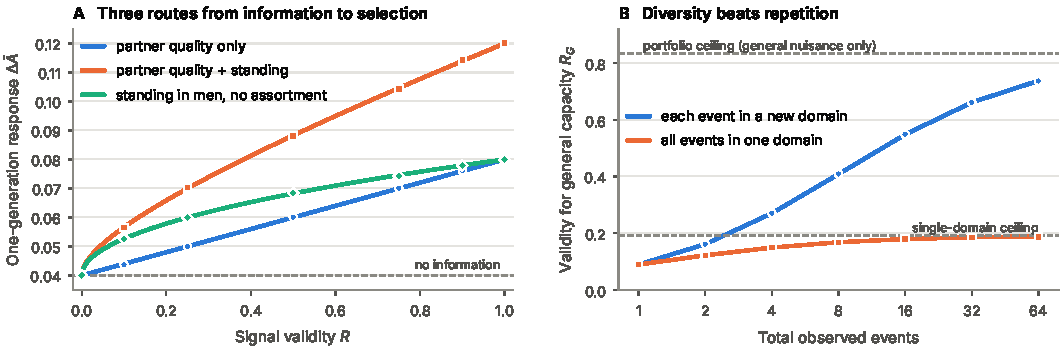
\includegraphics[width=\textwidth]{figures/figS1_routes.pdf}
\caption{\textbf{Routes and portfolios.} \textbf{(A)}~One-generation response under three routes ($V_A=0.4$, $V_P=1$): a
pair-output model ($b=0.2$); the same plus standing ($\beta_S=0.1$); and standing-dependent mating success in men
only ($\beta_N=0.1$, $\beta_S=0.2$), with no assortment. Lines: Eq.~\eqref{eq:threeroute}; markers: Monte Carlo means $\pm2$
standard errors (E2). \textbf{(B)}~Validity for general capacity when a fixed number of events is spread across new domains
or repeated within one; dashed lines are the ceilings of Proposition~\ref{prop:portfolio}. Parameters: $V_G=V_S=0.5$,
$\tau^2=0.5$, $\sigma^2=4$, $\rho=0.25$, $\omega^2=0.1$ (E3). Synthetic calculations, not estimates of human parameters.}
\label{fig:routes}
\end{figure*}

\subsection{Multigenerational amplification}

Fig.~\ref{fig:multigen} shows the individual-based simulation of Proposition~\ref{prop:assort}. With pair output $b=0.05$
and genic heritability 0.4, rank matching on observed scores raised additive variance to \MGva{} for initial validities
0.40, 0.67, 0.91, and 1, matching the recursion to within \MGerr\%. After 150 generations the cumulative response relative
to random pairing was \MGratio; the corresponding equilibrium amplifications are \MGF. The single-generation ceiling of two is
therefore not a ceiling on evolution. These ratios hold the pair-output coefficient fixed and so include the opportunity
increase that assortment creates. The genetic part is unambiguous: additive variance itself rose \MGinflLo- to
\MGinflHi-fold.

\begin{figure*}[t]
\centering
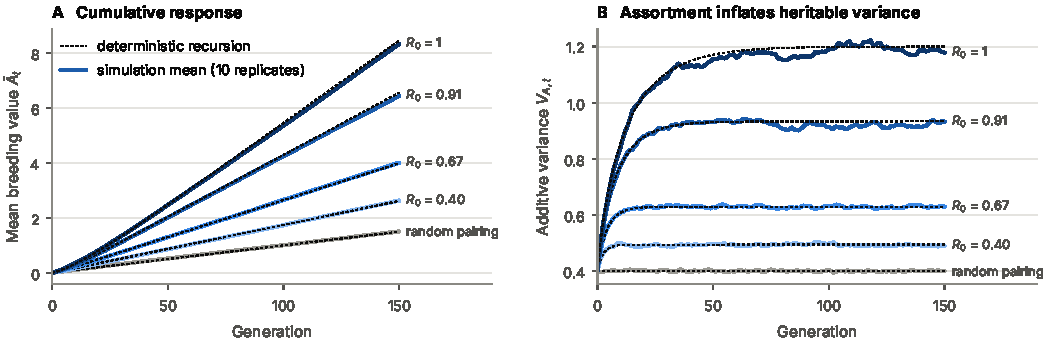
\includegraphics[width=\textwidth]{figures/figS2_multigen.pdf}
\caption{\textbf{Assortment across generations} (E4). Individual-based infinitesimal-model simulation: 5,000 individuals per
sex, 10 replicates, pair output $b=0.05$, $V_{LE}=0.4$, $V_E=0.6$. Partners are rank-matched on scores with fixed observation
noise; $R_0$ is the initial validity. Solid: simulation means; dotted: Eq.~\eqref{eq:assort} with mean response
$\tfrac b2V_{A,t}(1+m_t)$. Synthetic calculations.}
\label{fig:multigen}
\end{figure*}

\subsection{Decentralized matching and strategic non-display}

Ideal rank matching is a strong assumption. Experiment~E5 replaces it with men-proposing deferred
acceptance~\cite{gale1962} in which each person ranks potential partners by standardized score plus an idiosyncratic taste
term with standard deviation $s$. With common rankings ($s=0$) the stable matching gives $m=\DAmZero$ at $R=0.5$.
Idiosyncratic taste lowers the partner correlation, to \DAmOne{} at $s=1$ and \DAmTwo{} at $s=2$ (Table~\ref{tab:robust}), but
the response continues to follow $bV_A(1+m)/2$. The partner-quality route is thus governed by the realized phenotypic partner
correlation, a quantity measurable in any population. Non-display was modeled in two ways. When a random fraction $q$ do not
perform, validity falls to $(1-q)R$. When the lowest-scoring fraction hides and observers infer that hiders are below
average, validity falls much less (\HideThr{} instead of \HideRand{} at $q=0.4$), as disclosure unraveling
predicts~\cite{milgrom1981}.

\begin{table}[t]
\caption{Robustness to decentralized matching and non-display ($R=0.5$; E5).}\label{tab:robust}
\footnotesize
\begin{tabularx}{\columnwidth}{@{}Xccc@{}}
\toprule
\tabinput{generated/tab_robust.tex}
\bottomrule
\end{tabularx}
\end{table}

\subsection{Persistence, budget, and tissue}

Fig.~\ref{fig:persist}B verifies Proposition~\ref{prop:persist} in a finite population whose variance, validity, and
heritability evolve freely under the cost: the simulated equilibrium was \PersSim{} (between-replicate SD~\PersSD) against
\PersPred{} predicted from the realized $R$ and $V_P$. Fig.~\ref{fig:persist}A iterates Proposition~\ref{prop:tissue} with
$a=0.5$, $\kappa_K=0.01$, $\beta_{\mathrm{eff}}=0.04$, and tissue cost $\kappa_B$ halved three times. Both benefit types
begin with the same marginal value. Under positional demand, tissue investment doubles with each halving (\TisPos~SD), as
Eq.~\eqref{eq:tissue} predicts. Under saturating ecological demand, the same budget relaxations yield \TisEco~SD. When
positional returns are halved in the final phase (decoupling), tissue falls back to \TisBack~SD; the ecological trajectory is
unaffected. The time constant of each step is \TisApproachLo{} to \TisApproachHi{} generations, so at fossil resolution the
trajectory reads as stasis and steps.

\begin{figure*}[t]
\centering
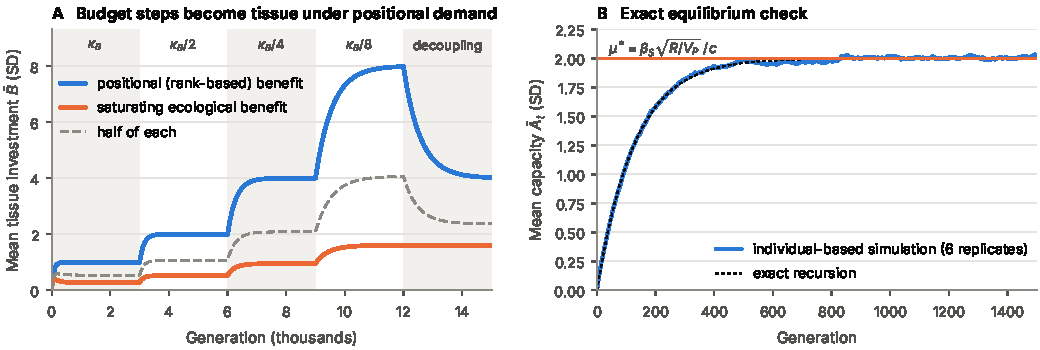
\includegraphics[width=\textwidth]{figures/figS3_persist.pdf}
\caption{\textbf{Persistence, budget, and tissue} (E6). \textbf{(A)}~Deterministic bivariate dynamics of
Proposition~\ref{prop:tissue}: tissue $B$ and organization $K$ with $\mathbf G=\mathrm{diag}(0.7,0.4)$, $a=0.5$,
$\kappa_K=0.01$, initial marginal benefit 0.04. Tissue cost $\kappa_B=0.02$ is halved at 3,000-generation intervals; in the
last phase positional returns are halved. \textbf{(B)}~Individual-based check of Proposition~\ref{prop:persist} (5,000 per
sex, 6 replicates, $c=0.02$, initial $R=0.5$); the horizontal line is Eq.~\eqref{eq:mustar} at realized $R$ and $V_P$.
Synthetic calculations, not fits to fossil data.}
\label{fig:persist}
\end{figure*}

\subsection{Contest, coalition, and aim}

Experiments E10--E12 check Model~V (Fig.~\ref{fig:contest}; Table~\ref{tab:modelv}). \emph{Aim.} Three illustrative regimes
weight three venues differently: a contest of force (loadings 1.0 on formidability and 0.25 on capacity), hunting (0.6 and
0.6), and verbal performance (0 and 1.0). With equal heritabilities, the simulated differentials match
Eq.~\eqref{eq:aim} under both an exponential rule ($\beta_S=0.2$) and a top-decile rule, and the ratio $S_{A_G}/S_{A_F}$ is
the same under both, as the proposition requires. Moving from the contest regime to skill and prestige raises selection on
capacity from \AimDomG{} to \AimPreG~SD and lowers selection on formidability from \AimDomF{} to \AimPreF. A cue in which 80\%
of the variance is a transient state yields a heritable response of only \CueSQ{} and no response in capacity
($|S_{A_G}|=\CueSG$, within one standard error of zero).

\emph{Repeatability.} With event noise four times the phenotypic variance, a single decisive contest has validity
\RepROne, against a ceiling of \RepCeil. As the cost per event falls from $\delta/B=0.2$ to $0.001$, the optimal number of
events rises from one to \RepNsafe{} and validity at the optimum to \RepRsafe, \RepFrac\% of the ceiling; at fixed intensity
the response is \RepGain{} times that of the single fight.

\emph{Leveling.} With subordinates' price $q=0.05$, a dominant tolerates no rivals until rival strength exceeds
$M=\DesThrLin$ fighter-equivalents under the linear law, or \DesThrSq{} under the square law. As $M$ grows his optimal share
falls toward \DesShareLin{} and \DesShareSq{} respectively, and the opportunity for selection among twenty males falls from
\DesIdespot{} to \DesILin{} and \DesISq.

\begin{figure*}[t]
\centering
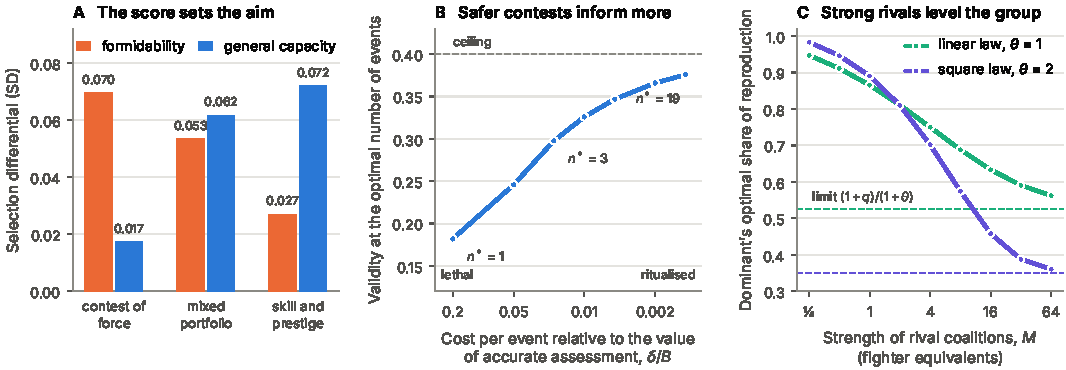
\includegraphics[width=\textwidth]{figures/figS4_contest.pdf}
\caption{\textbf{Contest, coalition, and aim} (E10--E12). \textbf{(A)}~Selection differentials on breeding values for
formidability and general capacity under three weightings of venues, at equal intensity (Proposition~\ref{prop:aim}).
\textbf{(B)}~Validity at the optimal number of contest events as the cost per event falls (Proposition~\ref{prop:repeat});
labels give $n^*$. \textbf{(C)}~The dominant's optimal share of reproduction as rival coalitions strengthen, with $q=0.05$
(Proposition~\ref{prop:despot}); dashed lines are the limits $(1+q)/(1+\theta)$. Loadings, costs and shares are
illustrative assumptions.}
\label{fig:contest}
\end{figure*}

\begin{table}[t]
\caption{Model~V illustrations (E10, E12). Loadings and shares are assumptions.}\label{tab:modelv}
\footnotesize
\begin{tabularx}{\columnwidth}{@{}Xccccc@{}}
\toprule
\multicolumn{6}{@{}l}{\textit{(a) Aim at equal intensity ($\beta_S=0.2$, $h^2=0.5$)}}\\
Regime & $\bar\ell_F$ & $\bar\ell_G$ & $S_{A_F}$ & $S_{A_G}$ & Ratio\\
\midrule
\tabinput{generated/tab_aim.tex}
\bottomrule
\end{tabularx}

\vspace{4pt}
\begin{tabularx}{\columnwidth}{@{}Xcccccc@{}}
\toprule
\multicolumn{7}{@{}l}{\textit{(b) The despot's dilemma ($q=0.05$; pool of 20 males)}}\\
 & \multicolumn{3}{c}{Linear law, $\theta=1$} & \multicolumn{3}{c}{Square law, $\theta=2$}\\
\cmidrule(lr){2-4}\cmidrule(l){5-7}
Rivals $M$ & $k^*$ & Share & $I$ & $k^*$ & Share & $I$\\
\midrule
\tabinput{generated/tab_despot.tex}
\bottomrule
\end{tabularx}
\tablenote{$k^*$: tolerated subordinates (integer optimum); Share: the dominant's share of group reproduction; $I$: opportunity
for selection among the 20 males, which is 19 when one male monopolizes reproduction.}
\end{table}

\subsection{The generalist target}

Experiment~E15 checks the results of Section~\ref{sec:generalist} (Figs.~\ref{fig:main}C and~\ref{fig:polymath}). With everyone compared on $K$
common domains, the simulated ratio of the selection differential on general capacity to that on one specialty is
\PolyRatioOne, \PolyRatioFour{} and \PolyRatioSixteen{} for $K=1$, 4 and 16, against exact values of 1, 4 and 16, while validity
for general capacity rises from \PolyValOne{} to \PolyValSixteen. When each individual is instead assessed only in the domain
of their greatest specific talent, the ratio is \PolyDivSimTen{} for ten specialties (exact, to first order in the strength of
selection, \PolyDivExTen), so common comparison aims \PolyDivTen{} times more strongly at general capacity than division of
labor does. Under a rule that honors each person's best performance while everyone is still seen in every domain, the
covariances are $V_G$ and $V_S/K$ as Stein's lemma requires, and only validity falls (from \PolySteinMean{} to \PolySteinMax{} at
$K=10$). In the individual-based evolution of a general investment and $K$ specific ones, the share of cost devoted to
general capacity matches Eq.~\eqref{eq:share} to within \PolyShareErr{} in all fifteen conditions, passing one half where the
number of domains equals the cost ratio.

\subsection{Tests and enforcement}

Experiment~E16 checks Section~\ref{sec:verification} (Figs.~\ref{fig:main}D and~\ref{fig:verify}A,B). Candidates were given a capacity, a default
rate drawn from a beta distribution with mean one quarter, and \VerN{} observed occasions split between staged and unstaged.
Simulated validities for capacity and for delivery agree with Eq.~\eqref{eq:staging} to within \VerMaxDiff{} at all seven
staging shares; the share that maximizes their product is \VerDstar, as Eq.~\eqref{eq:dstar} gives. For enforcement,
iterating the recursion for the means reproduces Eq.~\eqref{eq:enforceeq} to $\EnfRecErr$ both below and above the
threshold, and an individual-based population in which assessors shrink noisy signals of each trait settles within
\EnfIbmDiff{} of the predicted capacity and commitment at six levels of enforcement. With no enforcement and $T=\EnfT$
neither trait leaves zero; with complete enforcement capacity reaches its maximum and commitment stays at zero.

\subsection{Independent audit}\label{sec:auditnum}

A separate script re-derives each proposition by a different construction and imports no model code.
Proposition~\ref{prop:routes} was checked by constructing matched pairs directly from the conditional Gaussian distribution of
capacity given a shared score, with no sorting (40 blocks of 200,000 pairs; maximum $|z|=\AudZ$ across five validities);
Proposition~\ref{prop:persist} by 120-point Gauss--Hermite quadrature of the tilted density (maximum error $\AudQuad$);
Proposition~\ref{prop:assort} by comparing the quadratic root with fixed-point iteration (error $\AudRoot$, and divergence
confirmed where no equilibrium exists); Propositions~\ref{prop:portfolio} and~\ref{prop:aim} by explicit covariance algebra on
loading matrices (error $\AudCov$); Propositions~\ref{prop:repeat} and~\ref{prop:despot} by direct numerical maximization over
200 random parameter draws each (first-order residual $\AudFOC$; monotonicity confirmed; limiting share within $\AudAsym$);
and Proposition~\ref{prop:tissue} by iterating the dynamics for 20 random positive-definite $\mathbf G$ (equilibrium error
$\AudEq$, with tissue returning to zero when $a=0$). Corollary~\ref{cor:generalist} was checked by covariance algebra on
the loading vector and Proposition~\ref{prop:polymath} by iterating the dynamics for 20 random genetic covariance matrices
(error $\AudPoly$); the constants $c_K$ of Proposition~\ref{prop:division} by Monte Carlo (error $\AudCK$); and the
present-day decomposition by an independent implementation that reproduces every component of Table~\ref{tab:gss} checked to
$\AudGss$. Proposition~\ref{prop:delivery} was checked by Monte Carlo with $2\times10^6$ individuals (largest standardized
deviation \AudDelZ) and its threshold by the eigenvalues of 200 random systems, with no mismatch.
Proposition~\ref{prop:staging} was checked by exact summation over the default rate and the binomial count (error
$\AudStage$) and its optimum by bounded minimization (error $\AudStageOpt$); Proposition~\ref{prop:enforce} by Monte Carlo
covariances (largest standardized deviation \AudEnfZ), by solving the stationarity conditions directly in \AudEnfCases{}
random interior cases (error $\AudEnfEq$), and by eigenvalues of 400 random systems, with no mismatch. The speed-dating
results were recomputed from the raw file without the experiment's code: agreement between two observers by correlating
two randomly drawn observers of each person, a different estimator from the intraclass correlation (largest difference
\AudSpeedGap); the choice model with explicit chooser dummies in place of within-chooser centering (largest difference
$\AudSpeedLpm$ points); and expected and actual yeses by direct tabulation (identical). The ceiling of Eq.~\eqref{eq:ceiling} was checked by
simulating panels with shared error (largest difference \AudCeil). The audit detects coding
and algebra errors. It cannot validate
ancestral parameters or the historical interpretation.

Four further checks cover version 9. A14 verifies Proposition~\ref{prop:ancestors} by exact enumeration over discrete
family-size distributions, with no simulation (largest difference $\AudAnc$). A15 confirms that the three parts of the
decomposition of falling births sum to the change ($\AudBirths$) and that the directly computed effective numbers equal the
identity in the survey data. A16 recounts two cross-cultural variables from the raw file with a second reader that does
not use the same parser (difference in counts: \AudCultures). A17 recomputes, with a different reader, the number of
countries in the 175-country file in which women's ideal for a partner's financial prospects exceeds men's (difference:
\AudWorldSign).

\section{Mate selection today: stated, chosen, reproduced}\label{sec:today}

\noindent A present-day population cannot show what happened in the Pleistocene. It is, however, the only place where every
link of Section~\ref{sec:decomp} can be measured, and it shows which features of human mate selection persist when fertility
is controlled and which do not. Three bodies of evidence need to be kept apart: what people say they want, whom they choose,
and who has children.

\subsection{What people say they want}

Across 37 cultures, and again across 45 countries three decades later, women and men both rank kindness, intelligence and
health near the top; women give more weight to financial prospects and men to youth and attractiveness~\cite{buss1989,walter2020}.
When people must build a partner from a limited budget, physical attractiveness behaves as a necessity for men, status and
resources as necessities for women, and kindness and intelligence as necessities for both~\cite{li2002}; the ordering holds in
Eastern and Western samples~\cite{thomas2020}. Factor analyses of what people want in a partner return three dimensions:
warmth and trustworthiness, vitality and attractiveness, and status and resources~\cite{fletcher1999}; compatibility has
recently been proposed as a fourth, valued most in long-term contexts~\cite{jonason2026}.

\subsection{Whom people choose}

Stated preferences are a weak guide to choices. In speed dating, what people said they wanted did not predict whom they
picked~\cite{todd2007}. A meta-analysis of 97 studies of live and ongoing relationships found that physical attractiveness
predicted romantic evaluations at $r\approx0.40$ and earning prospects at $r\approx0.10$ in \emph{both} sexes, with sex
differences that were small and not significant~\cite{eastwick2014}. Machine-learning models given more than a hundred
self-reported traits and preferences predicted who was generally desired and who was generally desiring, but nothing about
which particular pairs clicked~\cite{joel2017}. In a registered report with 10,358 participants in 43 countries, the match
between a person's stated ideals and a partner's traits predicted how that partner was evaluated, but modestly
($\beta=0.19$ for the pattern across 35 traits, 0.11 beside a normative pattern, 0.04 on average for single traits); both
sexes understated how much attractiveness mattered to them, and women overstated, and men understated, how much earning
potential did~\cite{eastwick2025}. Across 11,196 couples, partners' personalities and traits added nothing to the
prediction of relationship quality beyond each person's own view of the relationship~\cite{joel2020}. The evidence is not
all one way: in a preregistered prospective study, preferences recorded while single did predict the characteristics of later
partners~\cite{gerlach2019}.

Several regularities do hold in behavior. Women in speed dating weighted intelligence more and men attractiveness more, and
men did not value a woman's intelligence or ambition once it exceeded their own~\cite{fisman2006}. In a field experiment that
sent invitations from constructed profiles on a large dating site, both sexes preferred attractive profiles; highly
educated women preferred highly educated men, and highly educated men preferred less educated women to the same degree,
so the two groups most likely to stay single were unattractive men with little education and unattractive women with
much~\cite{egebark2021}. Users of dating sites pursue partners more desirable than themselves~\cite{bruch2018}, yet stated
preferences alone, without search frictions, reproduce the sorting seen in marriages~\cite{hitsch2010}. Women's greater
selectivity is real but conditional: it grows with the number of candidates~\cite{fisman2006} and disappears when women are the
ones who approach~\cite{finkel2009}.

Spouses resemble each other. Partner correlations are positive across 22 traits~\cite{horwitz2023}, strongest for
education, attitudes and substance use; assortment on education and height leaves a detectable imprint on the
genome~\cite{yengo2018,robinson2017}. Educational homogamy in the United States rose from 1960 to 2003~\cite{schwartz2005}. In the
survey analyzed below the correlation between spouses' years of schooling was \GssHomOld{} in 1972--1989 and \GssHomNew{} in
2008--2024. As women's schooling has overtaken men's in most countries, the old pattern of women marrying
up in education has ended~\cite{esteve2016}.

\subsection{Said and done: \SdRows{} four-minute meetings}\label{sec:speed}

\emph{Data.} The Columbia speed-dating experiment~\cite{fisman2006} recruited \SdN{} graduate and professional students
(\SdW{} women, \SdM{} men; mean age \SdAge) to \SdSessions{} sessions in 2002--2004. Each pair talked for four minutes.
Each person then rated the other from 1 to 10 on attractiveness, sincerity, intelligence, fun, ambition and shared
interests, said whether they wished to meet again, and guessed how likely the other was to say yes. Before the event each
had divided 100 points among the six attributes. The public file has one row per person per meeting. We verified it by
checksum against four independent mirrors and reproduce the sample sizes of the original report. Variables describing race
and religion were not read.

\emph{Agreement.} Ratings were centered on each rater's mean, which removes leniency and differences among sessions.
Agreement between two observers of the same person, the one-way intraclass correlation, is \JurOneAtt{} for looks,
\JurOneFun{} for fun, \JurOneInt{} for intelligence, \JurOneAmb{} for ambition and \JurOneSin{} for sincerity
(Table~\ref{tab:speed}). Correlating the means of two disjoint random panels of $k$ raters reproduces the Spearman--Brown
curve from $k=1$ to 8 with a largest gap of \JurGapMax{} (Fig.~\ref{fig:main}B). The law is a statistical necessity when
errors are independent, so it should hold in any population. Independence is the condition that matters. Let $r_1$ be one
observer's squared correlation with the truth. If part of the error is common to all observers, so that their errors
correlate $c$, the error of a panel mean has variance $(1-r_1)[c+(1-c)/k]$, and the accuracy of the pooled verdict tends to
\begin{equation}
r_\infty=\frac{r_1}{r_1+c\,(1-r_1)}\label{eq:ceiling}
\end{equation}
however many observers are added: \JurCeil{} for a trait read as poorly as intelligence is here, at $c=0.3$. Shared error
also raises agreement, so consensus then overstates accuracy. In the experiment every rater met the person separately,
which is why the law fits; people who pass on one another's reports add voices and not observers. What a camp supplies is
many independent witnesses of many occasions. The single-observer agreements, unlike the law, need not travel, and here
they are lowered for intelligence by the narrow range of a sample selected for academic ability. Agreement does not differ by the
sex of the person rated for looks (\JurAttMen{} for men, \JurAttWomen{} for women) and is somewhat higher for men's fun
than for women's (\JurFunMen{} against \JurFunWomen).

\emph{Said and did.} Table~\ref{tab:speed} gives the points allocated before the event and the change in the probability
of a yes per standard deviation of each rating, from a linear probability model with a fixed effect for each chooser. The
model was fitted with the chooser's own ratings and again with the mean rating the partner received from everyone else,
which removes the chooser's halo. Either way looks come first for both sexes, then fun; intelligence earns one to four
points; sincerity and ambition earn none. In the sessions that asked, the day after, what had mattered in their decisions
($n=\SdAftN$), women put looks at \SdAftAttW\% and men at \SdAftAttM\%, well above what either had said beforehand, so the
gap between saying and doing is partly visible to the people themselves.

\emph{Legibility and weight.} Across the five attributes of a person, the effect of the panel's rating on a yes
correlates \SdLegPear{} with the agreement between two observers (rank correlation \SdLegSpear). Five points cannot
separate two readings: that people act on what they can read, or that what is easy to read happens to be what matters for
a first meeting. Prediction P27 separates them by lengthening the encounter and adding observers.

\emph{Access and misreading.} Women said yes to \SdYesW\% of partners and men to \SdYesM\%; \SdMatch\% of meetings ended
in a mutual yes. The share of partners who said yes to a person has a coefficient of variation of \SdPopCVM{} among men
and \SdPopCVW{} among women. Rescaling the 1--10 guess to 0--1, each sex expected a yes from \SdExpW\% of partners; women
received \SdActW\% and men \SdActM\%. The scale is arbitrary, but the sexes gave the same answer and met different
outcomes: men's expectation exceeded their outcome by \SdGapM{} points (\SdGapMCI), women's by \SdGapW{} (\SdGapWCI), a
difference of \SdGapDiff{} (\SdGapDiffCI). Men's overestimate of women's interest is what error-management theory predicts~\cite{haselton2000}. A speed-meeting
study designed to test it found the same in men and an underestimate in women~\cite{perilloux2012}, which these data do
not show. Within a person the guess correlates \SdAccM{} (men) and \SdAccW{} (women) with what the
partner decided.

\emph{Checks.} Self-ratings made before the event correlate \SdSelfAtt{} with the panel's verdict for looks, \SdSelfFun{}
for fun, \SdSelfAmb{} for ambition, \SdSelfInt{} for intelligence and \SdSelfSin{} for sincerity. The panel's rating of
intelligence correlates \SdSat{} (\SdSatCI; $n=\SdSatN$) with the median entrance-test score of the person's undergraduate
college, and its rating of looks \SdSatAtt. A speed date is a staged test in the sense of
Proposition~\ref{prop:staging}: everyone knows they are being assessed. The attribute closest to delivery, sincerity, is
the one that observers agree on least, that self-report tracks least, and that earns nothing.

\subsection{Desire, trust, and how relationships begin}\label{sec:desire}

Three further bodies of work bear on what is assessed. \emph{Desire.} Across 211 studies men report a stronger sex drive
than women ($g=0.69$; 0.54 after adjustment for biased responding), a difference between overlapping
distributions~\cite{frankenbach2022}. Willingness to accept a casual offer depends less on the sex of the person asked than on
who is asking: perceived sexual skill of the proposer predicted acceptance in both sexes, and the large sex difference of the
classic studies disappeared for some proposers~\cite{conley2011}. Within relationships, a partner's responsiveness raises
desire, more strongly in women, by making the other feel valued~\cite{birnbaum2016}. \emph{Trust.} What best predicts the
quality of a relationship is each person's perception of the other's commitment and appreciation; the partner's traits add
nothing further~\cite{joel2020}. Such perceptions are partly accurate and partly projection: in 107 couples, judgments of a
partner's willingness to increase intimacy tracked the partner's own report, while judgments of the partner's aversion to
deception did not and mainly reflected assumed similarity~\cite{wickham2020}. \emph{Beginnings.} In seven samples
($n=1{,}897$) about two-thirds of romantic relationships began as friendships, a route that research on initial attraction
between strangers largely overlooks~\cite{stinson2022}. Together these findings say that people assess two things, what a
partner can do and whether the partner will do it for them, and that the second is learned from conduct over time and not
from a first impression (Proposition~\ref{prop:delivery}).

The same two questions organize person perception in general. Perceivers judge others on warmth, read as intent, and on
competence, read as the ability to act on it~\cite{fiske2007}; moral character counts for more than warmth in the
impressions they form~\cite{goodwin2014}. The two are inferred by different rules. Models of impression formation assume a
negativity bias for morality and a positivity bias for competence, and experiments bear this out, the first most strongly
for extreme behavior and the second for moderate behavior~\cite{wojciszke1993,skowronski1987}. The logic is that of a
restrictive schema~\cite{reeder1979}: one skilled act is evidence of ability, since the unskilled cannot produce it, and
one dishonest act is evidence of character, since the honest do not. Occupational
psychology draws the same line between maximum and typical performance, which correlate about 0.4 in a meta-analysis, with
ability more strongly related to the first~\cite{beus2012,sackett1988}. Proposition~\ref{prop:staging} derives these rules
from what a recognized test can and cannot show. It also accounts for three features of courtship that preference lists
leave unexplained: that it takes time, which models treat as information bought by waiting~\cite{wachtmeister1999,seymour2009};
that women tend to underestimate men's commitment~\cite{haselton2000}; and that rivals disparage one another to prospective
partners~\cite{buss1990}, which supplies what a candidate would withhold.

\subsection{Context changes the weights, not the links}

What is weighted varies with circumstance. On tight budgets, Eastern and Western participants allocated differently for
almost every trait (average $d=0.42$) while still putting the same traits first~\cite{thomas2020}. Compatibility is weighted
more in long-term than in short-term contexts~\cite{jonason2026}. The sign of women's access component has reversed in
countries where earning and childbearing have been made compatible (Section~\ref{sec:gss}). A survey of 117,293 people in 175
countries is now public and allows such moderators to be tested directly~\cite{kowal2025}. Two limits apply. The decomposition
predicts that weights follow measurable conditions, such as insecurity, the burden of care and the availability of partners,
and not ancestry: sorting by group on a dating site reflects opportunity and expectation as well as preference, and users
who receive and answer a message across a racial boundary go on to start more such exchanges themselves~\cite{lewis2013}. And
this paper's own analyses compare no racial, ethnic or national groups, and nothing reviewed here supports ranking any.

Table~\ref{tab:culture} places the comparative evidence against the links. Its rows are published comparisons of
institutions and conditions, and each maps to a parameter of the models: who assesses, the share of occasions that are
unstaged, the enforced share of a candidate's product, the share of one sex left unpaired, the number of domains on which
everyone is compared, and the weight a partner's capacity carries. Three cautions apply to them. They are associations
across societies or communities, with the usual confounding. Stated preferences are the outcome in several, and stated
preferences are weak guides to choices (Section~\ref{sec:speed}). And where two large studies disagree, as on whether sex
differences in stated preferences shrink with gender equality~\cite{zentner2012,walter2020}, we report both. What the
table adds is a way to say what a cultural difference would have to change for selection to change: a society that moves
partner choice from kin to strangers, for example, alters the validity of delivery and leaves the validity of capacity
alone, and that is a testable statement (prediction P28).

\subsection{Who reproduces: an access--number decomposition}\label{sec:gss}

\emph{Data and method.} The General Social Survey has interviewed probability samples of United States adults since
1972~\cite{gss2024}. We use all \GssN{} respondents aged 45 to 79 born 1900--1979 with a known number of children, and four traits:
years of schooling, a ten-word vocabulary test, the prestige score of the respondent's occupation, and (for ages 45--64) the
logarithm of personal income. Each trait is standardized, and fitness made relative, within sex and decade of birth, so that
secular trends in schooling and family size do not enter. Eq.~\eqref{eq:split} then divides the selection differential into
access and number. Survey weights are applied; intervals are percentile bootstraps (\GssBoot{} resamples of respondents within
cells). The code reads the public file and reproduces every number here (Section~\ref{app:repro}).

\emph{The number component is negative for every trait in both sexes} (Table~\ref{tab:gss}, Fig.~\ref{fig:today}B). Among people who
become parents, those with more schooling, larger vocabularies, more prestigious occupations and higher incomes have fewer
children. Timing accounts for much of it. Each year's delay in the first birth goes with \GssTimSlopeW\% fewer children for
mothers and \GssTimSlopeM\% for fathers, schooling correlates \GssAfbRW{} (women) and \GssAfbRM{} (men) with age at first birth,
and the path through timing accounts for \GssTimShareW\% of the schooling--number relation in women and \GssTimShareM\% in men.

\emph{The access component has opposite signs in the two sexes.} For income it is $\GssIncMAcc$ (\GssIncMAccCI) in men and
$\GssIncWAcc$ (\GssIncWAccCI) in women; the difference, \GssIncDiffAcc{} (\GssIncDiffAccCI), is the largest contrast in the
table. Of men in the lowest third of income for their cohort, \GssChlMIncLo\% were childless, against \GssChlMIncHi\% in the
highest third; for women the figures run the other way, \GssChlWIncLo\% and \GssChlWIncHi\%. Occupational
prestige shows the same asymmetry at smaller size. For men's income the two components nearly cancel, leaving a total
differential indistinguishable from zero ($\GssIncMTot$; \GssIncMTotCI). A single correlation between status and fertility
would report ``no selection'' where there are two opposed episodes.

\emph{Three episodes, and the shape of the floor.} Access can be divided once more, into pairing (the mean trait of those who
ever married) and conversion (the further difference between parents and the ever-married); the three terms still sum to the
total (Table~\ref{tab:gssthree}). For men every trait is positive at pairing: income \GssIncMPair{} (\GssIncMPairCI), occupational
prestige \GssPreMPair, schooling \GssSchMPair{} and vocabulary \GssVocMPair. Conversion adds nothing for men's income
(\GssIncMConv) and is negative for schooling and vocabulary. For women no trait has a detectable effect at pairing, and
conversion is negative for all four. By fifths of income, men's childlessness is \GssQfMOne, \GssQfMTwo, \GssQfMThree{} percent in
the three lowest and \GssQfMFive{} in the highest, and the share never married falls from \GssNmMOne\% to \GssNmMFive\%
(Fig.~\ref{fig:today}A). The fall is concentrated at the bottom: the lowest-to-middle difference exceeds the middle-to-highest by
\GssFloorM{} percentage points (\GssFloorMCI). Marriage is an imperfect marker of pairing in recent cohorts, in which many
couples cohabit, so the pairing term is conservative for them.

\emph{The pattern is stable.} It appears in every birth cohort from 1900--1919 to 1960--1979, without weights, in the stricter
age window 50--74, and in surveys before and after 1990 (Tables~\ref{tab:gsscohort} and~\ref{tab:gssrobust}).

\emph{It is not new, and it is not peculiar to the United States.} British men with low incomes are more often childless
while women's income is negatively related to family size~\cite{nettle2008}; in European and United States samples the sex
difference in the status--fertility relation is driven by childlessness~\cite{fieder2007,barthold2012,hopcroft2006,weeden2006}; men
with higher incomes in the United States are more likely to marry, less likely to divorce and less likely to be
childless, and the reverse holds for women~\cite{hopcroft2021}. In Swedish registers the gradient of fertility on lifetime income is
strongly positive for men, and for women it has moved from negative to positive across cohorts born 1940--1970~\cite{kolk2023};
in the Nordic countries generally the negative gradient of women's education has vanished while the least educated men
remain the most often childless~\cite{jalovaara2019}. Swedish men with the lowest intelligence-test scores are the least likely
to have a first child~\cite{kolk2019}. What the present analysis adds is the exact split, for four traits and both sexes in one
sample, and its stability over eighty years of birth cohorts. The contrast across countries matters for interpretation: the
sign of the access term for women tracks institutions, since it has reversed where earning and childbearing have been made compatible. The
positive sign for men is found everywhere it has been looked for.

\emph{How much of the variance is the floor?} The opportunity for selection is $I=\GssIM$ in men and \GssIW{} in women, a small
sex difference of the size reported from other United States data~\cite{jokela2010}. Childlessness accounts for \GssShareM\% of it in
men and \GssShareW\% in women (Eq.~\ref{eq:oppsplit}), and the share has risen from \GssShareMOld\% and \GssShareWOld\% in cohorts
born 1920--1939 to \GssShareMNew\% and \GssShareWNew\% in those born 1960--1979 (Fig.~\ref{fig:today}E). As family sizes converge
on two, whether one becomes a parent at all carries a growing part of what variance remains.

\emph{The pairing gate.} Selection at pairing can act only on reproduction that passes through pairing, and the share that
does has fallen (Table~\ref{tab:gssgate}; Fig.~\ref{fig:verify}C). Among men born 1920--1939, \GssGateMOld\% (\GssGateMOldCI)
of those who never married were fathers, and never-married men accounted for \GssOutMOld\% of the children reported by men.
Among men born 1960--1979 the figures are \GssGateMNew\% (\GssGateMNewCI) and \GssOutMNew\%. For women they rose from
\GssGateWOld\% (\GssGateWOldCI) and \GssOutWOld\% to \GssGateWNew\% (\GssGateWNewCI) and \GssOutWNew\%. At the same time
the gate became more selective. The share of men never marrying rose from \GssNevMOld\% to \GssNevMNew\%, and the pairing
component of the differential on men's income rose from \GssPairMOld{} (\GssPairMOldCI) to \GssPairMNew{} (\GssPairMNewCI),
a change of \GssPairMChange{} (\GssPairMChangeCI). For women the pairing component moved from \GssPairWOld{}
(\GssPairWOldCI) to \GssPairWNew{} (\GssPairWNewCI), a change of \GssPairWChange{} (\GssPairWChangeCI): in the most recent
cohort women with higher incomes are slightly more likely to have married, where the pooled estimate of
Table~\ref{tab:gssthree} shows no effect. Event-history data likewise find that women's earnings became more important for
marriage formation between the early and late baby-boom cohorts~\cite{sweeney2002}. Two cautions apply. The survey records
marriage, not partnership, and most births outside marriage now occur to cohabiting couples, with a strong gradient by
education~\cite{lundberg2016}; and men may report children born outside marriage less completely than women do. The
cohort comparison was not planned in advance and should be read as description.

\emph{Standing and sexual partners.} Among respondents aged 45--79 the rank correlation between income and the lifetime
number of sexual partners of the other sex is \GssPartIncM{} (\GssPartIncMCI) in men and \GssPartIncW{} (\GssPartIncWCI)
in women; for vocabulary it is \GssPartVocM{} and \GssPartVocW, for schooling \GssPartSchM{} and \GssPartSchW, and for
occupational standing \GssPartPreM{} and \GssPartPreW{} (medians of \GssPartMedM{} partners for men and \GssPartMedW{} for
women). In this population a man's standing predicts whether he has a partner and whether he marries, not how many
partners he has; the small positive association in women is what later marriage would produce. Reported partner counts
are known to be biased, differently in the two sexes~\cite{mitchell2019}.

\emph{Marital history.} Table~\ref{tab:gsshist} and Fig.~\ref{fig:today}F give family size by marital history, relative
to the mean of the respondent's sex and decade of birth. Against people in a first marriage, remarried men have \GssRemM{} (\GssRemMCI) and
remarried women \GssRemW{} (\GssRemWCI), a sex difference of \GssRemDiff{} (\GssRemDiffCI). Men who divorced and did not
remarry have \GssDivM{} (\GssDivMCI), and \GssDivChlM\% of them are childless against \GssIntChlM\% of men in a first
marriage; for women the figures are \GssDivW{} (\GssDivWCI), \GssDivChlW\% and \GssIntChlW\%. The question about divorce
was put only to the currently married and widowed, and history is not randomly assigned: childless marriages end more
often. The asymmetry agrees with earlier findings that serial marriage raises men's reproductive success and not
women's~\cite{jokela2010}.

\emph{Who marries up.} Among currently married respondents the wife had more schooling than the husband in
\GssHypMoreOld\% of marriages of people born 1920--1939 and less in \GssHypLessOld\%; for those born 1960--1979 the figures
are \GssHypMoreNew\% and \GssHypLessNew\%, and for those born from 1980, \GssHypMoreYoung\% and \GssHypLessYoung\%
(a difference of \GssHypDiffYoung{} points; \GssHypDiffYoungCI; Table~\ref{tab:gsshyp}). The correlation between spouses'
schooling stayed near \GssHypR. In the oldest cohort, born 1900--1919, wives were also the more schooled spouse more often
than not, so husbands' advantage in schooling belongs to the middle of the century and is not a constant that recently
ended. The reversal follows the reversal of the sex gap in schooling and is seen
worldwide~\cite{esteve2016}.

\emph{Genetic evidence points the same way.} Polygenic scores for educational attainment are negatively associated with
number of children in Iceland, the United States and the United Kingdom, largely through later
childbearing~\cite{kong2017,beauchamp2016,hughjones2022,barban2016}; the association reverses once age at first birth is
controlled~\cite{hughjones2022}. On the access side, people who carry rare variants that damage genes under strong selective
constraint are more often childless, more so men than women, apparently because they are less likely to find a partner; the
authors estimate that this accounts for about a fifth of the purifying selection against such variants, while explaining less
than one percent of childlessness~\cite{gardner2022}.

\emph{Limits.} These are phenotypic differentials. They predict genetic change only to the extent that the covariance
between trait and fitness is genetic, which observational data cannot show~\cite{morrissey2010}. Income at ages 45--64 is partly
a consequence of family formation, with opposite effects on mothers' and fathers' earnings~\cite{kleven2019}; schooling is
mostly complete before childbearing and vocabulary is comparatively stable, which is why all four are shown. Respondents
are survivors to at least 45, number of children is top-coded at eight, and everything is self-reported. The estimates
describe one country. They carry no implication for the worth of any person or group and are no basis for policy.

\subsection{Sexual behavior: partners are not offspring}

Sexual selection theory expects reproductive success to rise with the number of mates, more steeply in
males~\cite{jones2009}. In this population it does not rise at all. Among adults aged 45--79, mean family size is highest
for those reporting exactly one lifetime partner of the other sex (\GssBatMOne{} children for men, \GssBatWOne{} for women) and
falls with each further category, to \GssBatMTwenty{} and \GssBatWTwenty{} for twenty or more (Fig.~\ref{fig:today}C). The slope of
relative fitness on relative partner number is \GssBatMGrad{} (\GssBatMGradCI) in men and \GssBatWGrad{} (\GssBatWGradCI) in women.
Reported counts are imperfect: men report more partners than women (medians \GssBatMMed{} and \GssBatWMed{} here), a gap that
estimation and social norms largely explain~\cite{mitchell2019}. The sign of the relation does not depend on such errors. With
effective contraception, status still predicts men's mating opportunities but not their fertility~\cite{perusse1993}, and what
predicts children is the time spent in a stable union: in a natural-fertility population, years married, not number of
partners, carried the relation between mating and reproductive success~\cite{borgerhoffmulder2019}.

Access, by contrast, has been tightening. At ages 22--34 the share reporting no sexual partner in the past year rose from
\GssPlMOld\% to \GssPlMNew\% among men and from \GssPlWOld\% to \GssPlWNew\% among women between 1989--2002 and 2016--2024
(Fig.~\ref{fig:today}D). Among men it is graded by income: \GssPlMLo\% in the lowest third against \GssPlMHi\% in the highest in the
latest period, and \GssPlMNone\% among men with no earnings. An analysis of the same survey for 2000--2018 found the rise
concentrated among unmarried men and associated with low income and with part-time or no employment~\cite{ueda2020}.

\subsection{Eight claims about present-day mate choice, checked}

Table~\ref{tab:audittoday} continues the audit of Table~\ref{tab:audit} for claims about the present.

\begin{table*}[t]
\caption{Eight common claims about present-day mate choice and selection, checked.}\label{tab:audittoday}
\scriptsize
\begin{tabularx}{\textwidth}{@{}P{0.028\textwidth}P{0.20\textwidth}P{0.10\textwidth}L@{}}
\toprule
 & Claim & Verdict & Evidence\\
\midrule
N11 & What people say they want is what they choose. & Weak guide &
Stated preferences did not predict speed-dating choices~\cite{todd2007}; attractiveness and earning prospects predict
evaluations about equally in both sexes whatever people state~\cite{eastwick2014}; pair-specific attraction is not predictable
from traits and preferences~\cite{joel2017}. Against this, preferences recorded while single predicted later partners'
characteristics in one prospective study~\cite{gerlach2019}.\\
\addlinespace
N12 & Women choose on status; men choose on looks. & Half right &
The difference in stated priorities holds across cultures~\cite{buss1989,walter2020,li2002}. In live evaluation both sexes
respond mainly to attractiveness~\cite{eastwick2014,egebark2021}. Where the sexes differ is in outcomes: income raises men's chances
of marriage and fatherhood and lowers women's chances of motherhood (Table~\ref{tab:gss})~\cite{nettle2008,hopcroft2021}, and
education preferences in a field experiment had opposite signs~\cite{egebark2021}.\\
\addlinespace
N13 & Intelligence is attractive. & Perceived, not measured &
Measured intelligence can be detected from videos and in live interaction but does not raise attractiveness; perceived
intelligence and funniness do~\cite{driebe2021}. Humor ability tracks intelligence and predicts mating
success~\cite{greengross2011}. Men did not value women's intelligence above their own~\cite{fisman2006}. General capacity reaches
choice through performance and standing more than through direct attraction.\\
\addlinespace
N14 & Women are the choosy sex. & Conditional &
Women are more selective in most settings, more so with more candidates~\cite{fisman2006}; the difference vanished when women
approached and men sat~\cite{finkel2009}. Human mating does not follow one universal pattern of sex roles~\cite{brown2009}, both
sexes choose~\cite{stewartwilliams2013}, and in most small-scale societies kin choose too~\cite{walker2011}.\\
\addlinespace
N15 & Women's preferences shift toward masculine men when fertile. & Not supported &
A meta-analysis of 58 reports was largely nonsupportive, with effects confined to published studies using imprecise
definitions of the fertile phase~\cite{wood2014}; a large longitudinal study with hormone assays found no relation between
hormonal status and preference for facial masculinity~\cite{jones2018}.\\
\addlinespace
N16 & Masculine faces and deep voices mark the men who reproduce most. & Mostly not &
Across 96 studies, strength and muscularity were the only consistent predictors of both mating and reproduction; voice
pitch, height and testosterone predicted mating only, and facial masculinity predicted neither~\cite{lidborg2022}.\\
\addlinespace
N17 & For men, more partners mean more offspring. & Not now &
Family size peaks at one lifetime partner in both sexes and declines thereafter (Fig.~\ref{fig:today}C). Status predicts men's
mating opportunities but not fertility under contraception~\cite{perusse1993}. Men with three or more successive spouses had 19\%
more children than men with one, with no such effect in women~\cite{jokela2010}: unions, not partners, are what count.\\
\addlinespace
N18 & Selection on humans has stopped; or, intelligence is being bred out. & Neither &
Selection continues on many traits~\cite{byars2010,sanjak2018,gardner2022,akbari2026}. On education-linked variants it is negative
and slow, about 0.01 standard units per decade in Iceland~\cite{kong2017}, too slow to account for more than a small part of
observed change~\cite{beauchamp2016}. Test-score trends in both directions arise within families and are
environmental~\cite{bratsberg2018}; brain volumes rose across twentieth-century birth cohorts~\cite{decarli2024}.\\
\bottomrule
\end{tabularx}
\end{table*}

\section{Questions raised in review, and what the evidence says}\label{sec:notes}

Review of the previous version raised ten questions. Each is stated here with the evidence found, a verdict, and the
change it made to the paper. New analyses are experiments E18--E21 (Section~\ref{sec:experiments}); new formal results are
in Section~\ref{sec:modelix}.

\subsubsection{1. Does ``female choice'' assume consent? Was rape common}
\emph{Evidence.} Table~\ref{tab:cultures} gives every relevant code in the Standard Cross-Cultural Sample. A daughter
chooses alone in \CcAloneW\% of societies; her consent is unnecessary in two-thirds of those with information; rape is
reported in about half of the societies coded for it by one team and rated common in \CcRapeCom{} of \CcRapeN{} by another;
captives, wife-beating and unequal access to divorce are all recorded. Among the \CcRapeParN{} societies coded for both,
rape is rated common in \CcRapeParCom{} where parents choose a daughter's husband and in \CcRapeOwnCom{} of \CcRapeOwnN{}
where she chooses; the numbers are too small to bear weight. Low rates of extra-pair paternity in historical
populations~\cite{larmuseau2016} bound conceptions outside recognized unions, not coercion within them. Male aggression
against women has a comparative and evolutionary literature of its own~\cite{smuts1992}, and raiding for women is described
ethnographically~\cite{chagnon1988}. \emph{Verdict.} The objection is right about the word and does not touch the
mechanism. No rate of coercion can be given for the Pleistocene. \emph{Change.} The paper no longer writes of choice by
women where it means decision by whoever decides; Eq.~\eqref{eq:coercion} states what coercion does to the pathway;
Section~\ref{sec:reschoice} reports the record; objection O45 and prediction P30 follow.

\begin{table*}[t]
\caption{Who decides a marriage, and how much constraint and coercion is coded, in the Standard Cross-Cultural Sample and in
Binford's hunter-gatherer compilation (D-PLACE release~\cite{kirby2016}). Counts and shares of societies with a code; no
significance is claimed across societies, which share ancestry and neighbors.}\label{tab:cultures}
\scriptsize
\begin{tabularx}{\textwidth}{@{}P{0.24\textwidth}P{0.10\textwidth}rL@{}}
\toprule
\tabinput{generated/tab_cultures.tex}
\bottomrule
\end{tabularx}
\end{table*}

\subsubsection{2. Did only half of all men reproduce? Is there twice as much female DNA}
\emph{Evidence.} The claim descends from the twofold deeper coalescence of mitochondrial than Y-chromosome
lineages~\cite{wilder2004} and was popularized as ``80\% of women and 40\% of men''~\cite{baumeister2010}. Later work with
complete sequences confirms larger differences among populations for the Y chromosome, with regional variation and smaller
effects than first reported~\cite{lippold2014}; X-linked diversity is higher than expected relative to
autosomes~\cite{hammer2008}; a recombination-based estimate puts the breeding ratio nearer one than two~\cite{labuda2010}; and a
bottleneck in Y lineages within the last ten thousand years~\cite{karmin2015} is explained by competition among patrilineal
kin groups without any change in how many men fathered children~\cite{zeng2018}. Across societies with data, the variance
in men's reproductive success exceeds women's by amounts that depend on the marriage system~\cite{brown2009,betzig2012}.
\emph{Verdict.} Half right. Men's reproduction has been the more unequal; the headcount is not recoverable from the ratio
(Proposition~\ref{prop:ancestors}); and autosomal DNA comes equally from mothers and fathers in every generation, so the
second claim is false as stated. \emph{Change.} Proposition~\ref{prop:ancestors}, Fig.~\ref{fig:choice}D, estimates for
the United States, and the link to the floor (Corollary~\ref{cor:floor}).

\subsubsection{3. Did \textit{Homo floresiensis} live beside australopiths, or alone on an island}
\emph{Evidence.} Neither beside australopiths nor beside anyone. The Liang Bua remains date to about 100,000--60,000 years
ago~\cite{sutikna2016}; similar hominins were on Flores by 0.7 million years ago~\cite{brumm2016,vandenbergh2016}; a second
small-bodied island species is known from Luzon~\cite{detroit2019}. The last australopiths lived more than a million years
earlier, in Africa. The brain of \textit{H.~floresiensis} is of australopith size~\cite{kubo2013}, which is the source of
the confusion and was the point of plotting it. \emph{Verdict.} The earlier wording (``persisted beside large-brained
ones'') invited the misreading. \emph{Change.} Text corrected in Sections~\ref{sec:resfossil} and~\ref{sec:reshominins};
isolation is now part of the explanation offered.

\subsubsection{4. Was attention deficit an advantage for hunter-gatherers? Is there a 20\% figure}
\emph{Evidence.} Section~\ref{sec:reshominins} gives the five findings we could verify~\cite{ding2002,matthews2011,eisenberg2008,barack2024,esteller2020}
and one theory of how a minority strategy could persist~\cite{williams2006}. The Ariaal study compared 65 nomadic and 87
settled men and found body mass index higher in carriers of the \textit{DRD4} 7R allele among nomads and lower among the
settled, mainly through fat-free mass; it reports no percentage advantage in efficiency. \emph{Verdict.} Plausible for
exploration-related traits in mobile settings; unsupported as a claim that a clinical condition was selected for; the 20\%
figure could not be traced. \emph{Change.} Corollary~\ref{cor:narrow} states what the framework can say: a mixed profile is
neutral under broad comparison and a deficit under a narrow test. Prediction P33 tests it.

\subsubsection{5. Brains shrank while cognitive alleles rose: doing more with less}
\emph{Evidence.} Both parts hold with caveats: a decline of more than 5\% in 50,000 years, largely tracking body
size~\cite{stibel2021,ruff1997}, with the timing of any later drop disputed~\cite{desilva2021,villmoare2022}; and a
one-standard-deviation rise over ten thousand years in combinations of alleles that predict cognitive measures
today~\cite{akbari2026}. Selection for prosociality, likened to domestication, has also been proposed for recent human
evolution~\cite{hare2017}. \emph{Verdict.} Compatible, and predicted by Proposition~\ref{prop:tissue} when tissue is costly. The
comparison with efficient machine-learning models is an analogy of form. \emph{Change.} A paragraph in
Section~\ref{sec:reshominins} and a statement in Section~\ref{sec:ai}.

\subsubsection{6. Was neurodivergence selected for the forest: sharper senses, attention, smell}
\emph{Evidence.} Hunter-gatherers name odors far better than neighboring horticulturalists who speak a closely related
language~\cite{majid2018}, which attributes the difference to way of life. Common variants associated with autism show
signatures of positive selection, which the authors relate to cognitive ability~\cite{polimanti2017}. We found
no study showing heritable sensory acuity that was favored in foragers and relaxed in farmers. \emph{Verdict.} Not
supported as stated. Diagnostic categories are modern and should not be projected onto past populations. \emph{Change.}
One sentence in Section~\ref{sec:reshominins}.

\subsubsection{7. Do storytellers have more children? What of social networks, fire, and staying up late}
\emph{Evidence.} Yes for Agta storytellers~\cite{smith2017}, for network position among Agta and BaYaka
mothers~\cite{page2017}, and for cooperative ties among the BaYaka~\cite{chaudhary2016}; Hadza networks are structured by
cooperation~\cite{apicella2012}; firelit talk is stories~\cite{wiessner2014,dunbar2014}, and people without electricity
stay awake some hours after dark~\cite{yetish2015}. Status of several kinds goes with men's reproductive success across
33 nonindustrial societies~\cite{vonrueden2016}. We could not identify the book cited to us as \emph{Outbound}. \emph{Verdict.}
Supported, and it enters the model in two places that the cooking hypothesis does not: fire raises the number of occasions
and observers (Eq.~\ref{eq:sb}) and adds speech as a domain of common comparison (Corollary~\ref{cor:generalist}).
\emph{Change.} A paragraph in Section~\ref{sec:resjury}; prediction P31.

\subsubsection{8--9. The Maasai: lion hunting replaced by jumping; safe, repeatable rituals}
\emph{Evidence.} The tournament exists and was created for that purpose~\cite{maasaiolympics,aljazeera2022}; lion killing by
Maasai has several motives, of which the warrior's proof is one~\cite{hazzah2009,goldman2013}; marriage by custom follows
the ceremony that ends warriorhood~\cite{aljazeera2023,spencer1988}. Ritual fights raise men's reproductive success among the
Sereer~\cite{llaurens2009}, sports are overwhelmingly male in 50 societies~\cite{deaner2013}, and games with winners are
nearly universal (\CcGamesAny{} of \CcGamesN{} societies; \CcGamesForAny{} of \CcGamesForN{} foraging societies). We report
only the presence of games~\cite{roberts1959}: the distribution of types in the release looked implausible to us (most
foraging societies coded as having games of strategy alone), and we could not check it against the source. \emph{Verdict.} Supported as a case of substitution.
That jump height decides eligibility to marry is not supported by any source we found; prestige is what is at stake.
\emph{Change.} Corollary~\ref{cor:ritual}, a paragraph in Section~\ref{sec:rescontest}, prediction P32.

\subsubsection{10. Specialization, online life, the loss of community, and falling births}
\emph{Evidence.} Tables~\ref{tab:births} and~\ref{tab:village}. Ideals have not moved; the fall in children per young
adult is accounted for almost wholly by the rise of the never married; social evenings with neighbors and friends, and
weekly worship, have declined; time online has risen; having no partner has become commoner, especially for men. Against
the simple story: seeing friends goes with being single, time on social media is unrelated to being single in 70
countries, and couples who met online married sooner in one panel~\cite{rosenfeld2017}. Completed fertility falls short of
intentions in Europe and the United States generally~\cite{beaujouan2019}, and social networks shape fertility
decisions~\cite{bernardi2014}. \emph{Verdict.} Supported at the level of accounting and trend; the causal step from thin
community to fewer unions is conjecture, formalized as Proposition~\ref{prop:waiting}. On generalists: the model says
division of labor removes the premium on general ability (Proposition~\ref{prop:division}); it does not say generalists
survive better. \emph{Change.} Section~\ref{sec:resvillage}, Fig.~\ref{fig:village}, predictions P34 and P35, objection O49.

\begin{table*}[t]
\caption{Marriage, children and ideals among adults in the General Social Survey. Children and marital status: ages
25--39. Ideal number of children for a family: ages 18--44, answers of ``as many as you want'' excluded. Weighted.}\label{tab:births}
\scriptsize
\begin{tabularx}{\textwidth}{@{}lrCCCCC@{}}
\toprule
\tabinput{generated/tab_births.tex}
\bottomrule
\end{tabularx}
\end{table*}

\begin{table*}[t]
\caption{Social ties and partnership among adults aged 22--34, by survey period (General Social Survey; percentages unless
stated; weighted). Questions on partners began in 1988 and on time online in 2000. Surveys from 2021 were partly
self-administered.}\label{tab:village}
\scriptsize
\begin{tabularx}{\textwidth}{@{}Lrrrrr@{}}
\toprule
\tabinput{generated/tab_village.tex}
\bottomrule
\end{tabularx}
\end{table*}

\begin{table*}[t]
\caption{Stated ideals and partnership across countries. K: 175-country survey~\cite{kowal2025}, countries with at least 50
men and 50 women (150 of each for the partnership row). W: 45-country survey~\cite{walter2020}. Differences $d$ are in pooled
standard deviations. No country is named or ranked.}\label{tab:world}
\scriptsize
\begin{tabularx}{\textwidth}{@{}LcrP{0.34\textwidth}@{}}
\toprule
\tabinput{generated/tab_world.tex}
\bottomrule
\end{tabularx}
\end{table*}

\subsubsection{The conclusions were not strong or important enough}
The earlier version reported what could be derived and measured and stopped. This one states eight conclusions and marks
the status of each (Section~\ref{sec:conclude}). The two with the widest consequences are that the reading of minds is a
property of communities, and that the births now missing in the United States are missing at the step where a couple
forms. Both are stated as strongly as the data allow and no more strongly: the first is measured and derived, the second
is an accounting in one country with a conjectured mechanism and three findings against its simplest form.

\subsubsection{Further open data examined}
Of fifty candidate sources suggested to us, two were added as analyses: the 175-country survey~\cite{kowal2025}, licensed
CC~BY~4.0, and the 45-country survey~\cite{walter2020} (Table~\ref{tab:world}; E20). Published findings on length of
acquaintance~\cite{hunt2015} and on romance that begins as friendship~\cite{stinson2022} were added as evidence. Public-domain
deposits of face-rating data could not be downloaded in our build environment, and panels that require a signed agreement
(on how couples meet, and national fertility surveys) were not used; they are the natural next tests of predictions P28,
P34 and P35.

\section{Nine selection drivers: the evidence}\label{sec:hidden}

\noindent This section gives the evidence behind each driver in Table~\ref{tab:drivers}. One driver is common to both sexes and
four are specific to each. All are supported by the evidence cited; none is established as a cause of brain expansion, and each
is paired with a prediction that could count against it.

\begin{table*}[t]
\caption{Nine selection drivers: what each acts on, through which episode and assessor, and whether it still operates.
``Then'' summarizes field evidence from small-scale and historical populations; it is not a reconstruction of the Pleistocene.}
\label{tab:drivers}
\scriptsize
\begin{tabularx}{\textwidth}{@{}P{0.135\textwidth}P{0.16\textwidth}P{0.115\textwidth}LP{0.19\textwidth}P{0.05\textwidth}@{}}
\toprule
Driver & Acts on & Episode; assessor & Then & Now & Test\\
\midrule
G. Generalist target (both sexes) & What many performances share: general capacity and condition & Access and standing;
everyone who watches & Broad common repertoire in small groups~\cite{schniter2015}; leaders marked by expertise and
knowledge~\cite{garfield2019} & Division of labor narrows comparison to one occupation & P2, P22, P26\\
M1. Floor & The low tail: mutational load, incapacity & Access; partners and their kin & Excess male variance from mating
success~\cite{courtiol2012} & Operating at pairing: childlessness concentrated at the bottom of men's income distribution (Fig.~\ref{fig:today}A); damaging
variants and childlessness~\cite{gardner2022} & P17, P21\\
M2. Jury of elders and allies & Reliability, competence, cooperation & Access; in-laws and coalition & Arranged
marriage~\cite{walker2011}; standing and reproduction~\cite{vonrueden2016} & Weakened where partners choose alone & P7, P19, P24\\
M3. Controlled strength & Self-control with formidability & Access and survival; coalition & Leveling of dominants~\cite{boehm1993};
reduced reactive aggression~\cite{wrangham2019} & Strength still predicts mating and reproduction~\cite{lidborg2022} & P13, P15, P25\\
M4. Being kept & Investment, dependability & Number; wives and their kin & Years married drive reproductive
success~\cite{borgerhoffmulder2019} & Operating: income, lower divorce, remarriage~\cite{hopcroft2021} & P18\\
\addlinespace
F1. Keeping children alive & Knowledge, competence, standing & Offspring survival; no assessor needed & Maternal knowledge and
influence predict child health~\cite{mcdade2007,alami2020} & Idle: almost all children survive & P18\\
F2. Recruiting help & Social cognition, alliance & Offspring survival; kin and allies & Relatives improve child
survival~\cite{sear2008} & Largely replaced by institutions & P18\\
F3. Chosen for work and character & Industry, competence, character & Partner quality; husbands and their kin & Hadza men value
hard work~\cite{marlowe2004} & Operating through assortment on education~\cite{horwitz2023} & P6\\
F4. Timing & Age at first birth & Timing; the couple and kin & Earlier-starting wives~\cite{vonrueden2011} & Operating, sign
reversed for schooling (Table~\ref{tab:gss}) & P20\\
\bottomrule
\end{tabularx}
\end{table*}

\subsection{Shared: the generalist target}

Selection through assessed standing falls on what a person's performances have in common
(Corollary~\ref{cor:generalist}), and the conditions for that were met in small societies: Tsimane adults command a broad
range of skills across food production, child care, craft, music and storytelling, acquire most of the essential ones before
first reproduction, and report their own skill levels accurately~\cite{schniter2015}. The general factor that such comparison
rewards has a biological counterpart. Across 62 primate species, innovation, social learning, tool use, extractive
foraging and tactical deception form a single composite that covaries with brain volume~\cite{reader2011}; evidence for a
general factor extends to other mammals~\cite{burkart2017}; and within humans the genetic influences on different cognitive
abilities largely overlap~\cite{kovas2006,plomin2015}. The cortex that expanded most in the human lineage is association cortex,
which also expands most after birth~\cite{hill2010,buckner2013}, and a fronto-parietal network is recruited by demanding tasks of
every kind~\cite{duncan2010}. Ecology pushed the same way: our species occupied a wider range of environments than any other
hominin~\cite{roberts2018}, as variability selection would favor~\cite{potts1998}, and among birds larger-brained species do better
in novel environments~\cite{sol2005}. What the assessment model adds to these accounts is a reason for the generalist
to be favored within groups, generation after generation, and a reason for that favor to fade: specialization
(Proposition~\ref{prop:division}). Hunters already sort themselves into the tasks at which they are most
efficient~\cite{hooper2015}; full occupational division of labor is a Holocene development.

\subsection{Men}

\emph{M1. The floor, not the podium.} Selection on men acts mainly by exclusion at the low end. In historical Finland variance
in mating success explained most of men's excess variance in fitness~\cite{courtiol2012}; in present-day Britain, Sweden, the
Nordic countries and the United States, low income, low test scores and little education go with male childlessness
(Section~\ref{sec:gss}); and carriers of rare damaging variants are more often childless, men especially, apparently for want
of a partner~\cite{gardner2022}. A floor is cheap to operate, since everyday life supplies the information it needs
(Corollary~\ref{cor:floor} and the remark following it), and it is the form of sexual selection best suited to clearing
deleterious mutations, most of which should lower male mating success~\cite{whitlock2009,lumley2015}. A brain to which a large
fraction of the genome contributes is an exposed target for exactly that filter~\cite{keller2006}.

\emph{M2. The jury of elders and allies.} A young man in a foraging society was judged less by a prospective bride than by her
parents, who arranged most marriages~\cite{walker2011,apostolou2007}, and by the men whose support decided his
standing~\cite{vonrueden2016,henrich2001}. Parents favor investment and cooperation over the signs of heritable quality that their
children favor~\cite{buunk2008}. Men were therefore selected for what older adults and peers value after years of
observation: competence, reliability and usefulness to others. This is assessment by record, the kind for which validity is
highest (Proposition~\ref{prop:portfolio}), and it is the only kind that reaches delivery: a suitor can perform for a
bride, but what he does on days when no one is being courted is seen by the people who live beside him
(Proposition~\ref{prop:staging}).

\emph{M3. Controlled strength.} Strength and muscularity are the one set of masculine traits that predict both mating and
reproduction~\cite{lidborg2022}, yet coalitions punish men who dominate by force~\cite{boehm1993,wrangham2018}, anatomy suggests
selection against reactive aggression over the last 300,000 years~\cite{wrangham2019,cieri2014}, and both sexes treat kindness as a
necessity in a partner~\cite{li2002}. The target was formidability under control: dangerous to rivals, safe for partners and
allies. Self-control is a general cognitive capacity, and leveling is what made it pay (Proposition~\ref{prop:despot}).
Leveling also enforced delivery. Where what a strong or able man produced was claimed by others whatever his disposition,
his capacity was worth conferring standing on before any inclination to share had evolved
(Proposition~\ref{prop:enforce}).

\emph{M4. Being kept.} What converts mating into offspring is time in a union. Years married, not number of partners, carried
the relation between mating and reproductive success in a natural-fertility population~\cite{borgerhoffmulder2019}; in the
United States men with higher incomes are less likely to divorce and more likely to remarry~\cite{hopcroft2021}, and serial
marriage raises men's family size~\cite{jokela2010}. Paternal investment of the human kind is unusual among
mammals~\cite{geary2000,marlowe2000}. Men were selected to be worth retaining, by wives and by wives' kin, over decades.

\subsection{Women}

\emph{F1. Keeping children alive.} With high infant and child mortality~\cite{volk2013}, variance in women's fitness lay less in
births than in survivors. A Tsimane mother's plant knowledge predicts her children's health~\cite{mcdade2007}, and her political
influence predicts their growth and freedom from illness after adjustment for wealth and kin~\cite{alami2020}. Selection on
women's competence, knowledge and standing was direct and did not depend on anyone's choice of them.

\emph{F2. Recruiting help.} Human mothers raise overlapping dependents with help from kin and
others~\cite{kramer2010,hawkes1998,burkart2014}; in almost every population studied at least one relative besides the mother
improves child survival~\cite{sear2008}. Help has to be negotiated and kept. Women compete for partners and for resources, mostly by
low-risk means~\cite{stockley2013}, and the stake was the survival of children. This is a route for selection on social
cognition in women through the survival episode, independent of mate choice by men.

\emph{F3. Chosen for work and character, not shape.} Men choose too~\cite{stewartwilliams2013}. Hadza men look for hard work in a
wife and both sexes rate character highly~\cite{marlowe2004}, while the body cues popularly read as signs of fertility have
little measured validity (claims N9 and N10). A woman's assessed qualities affected whom she married more than whether, so the
route is partner quality (Proposition~\ref{prop:routes}), sustained by assortment (Proposition~\ref{prop:assort}).

\emph{F4. Timing.} When childbearing begins is the main lever on women's family size once access is nearly universal.
Prestigious Tsimane men gain chiefly through wives who start earlier~\cite{vonrueden2011}; in Framingham women selection favors an
earlier first birth~\cite{byars2010}; variants associated with age at first birth in women are associated with reproductive
success~\cite{sanjak2018}. Today the same lever, pulled the other way by schooling, carries most of the negative relation between
women's education and family size (Section~\ref{sec:gss}).

\subsection{What the drivers have in common}

Each moves selection away from a contest for the most desirable partner and toward judgments that many people make about
ordinary conduct over a long time: whether a man is acceptable at all, whether he is worth keeping, whether a woman's children
thrive and whether others will help her. Those judgments load on general, social and self-regulatory capacities; they rest
on records and not on cues; and they are made by people with years of observation behind them. That is the setting in which
the information--opportunity identity gives its largest product for a general-purpose brain: validity is at its highest,
the aim is on what performances share, and modest floors supply all the intensity the fossil rate requires.

\section{Is the engine still running?}\label{sec:present}

\noindent The identity of Proposition~\ref{prop:identity} gives a way to ask whether the hypothesized drivers still operate,
factor by factor (Table~\ref{tab:eras}).

\begin{table*}[t]
\caption{The factors of the identity in three eras. The first column is historical conjecture; the others summarize cited
evidence.}\label{tab:eras}
\scriptsize
\begin{tabularx}{\textwidth}{@{}P{0.12\textwidth}LLL@{}}
\toprule
Factor & Pleistocene foragers (conjectured) & Holocene agrarian and state societies & Societies after the demographic
transition\\
\midrule
Accuracy ($h\sqrt R$) & Years of direct observation across many venues, pooled by talk & Mixed: reputation within
communities, but rank increasingly fixed by birth & Abundant records (schooling, examinations, credentials); accuracy relative to years of direct observation is unmeasured\\
Aim (what standing loads on) & Many common domains: skill, knowledge, generosity, courage; force held in check by leveling &
Wealth, descent group, office; force returns with states; occupations specialize & One occupation per person; education and
occupation load on cognitive ability\\
Intensity and alignment & Modest skew; standing aligned with reproduction through marriage timing, remarriage and support
& High skew among men, aligned with inherited wealth and power~\cite{karmin2015,zeng2018,borgerhoffmulder2009} & Low skew;
alignment split by episode: access still favors men's status, number runs against schooling and status in both sexes
(Table~\ref{tab:gss})~\cite{reeve2018,kong2017,beauchamp2016,hughjones2022}\\
Genetic variance & Assortment on assessed standing & Assortment within strata & Strong assortment on education and ability
($m\approx0.4$--0.55)~\cite{horwitz2023}\\
Energy budget & Binding; relaxed in steps by cooking, provisioning, shared care & Binding for most; bodies and brains
smaller~\cite{ruff1997} & Slack for most; obstetric constraint eased by surgery~\cite{mitteroecker2016}\\
\midrule
Net effect on capacity & Weak, persistent, positive & Uncertain; allele frequencies suggest positive in West
Eurasia~\cite{akbari2026} & Near zero or weakly negative, varying by sex and setting\\
Net effect on tissue & Positive when the budget allowed & None or negative & None detected; cohort gains are
developmental~\cite{decarli2024}\\
\bottomrule
\end{tabularx}
\end{table*}

\emph{Tissue stopped first.} Endocranial volume in \Hs{} has not risen for at least 100,000 years and probably 300,000
(Section~\ref{sec:explananda}); recent populations average \RecentDrop\% less than terminal Pleistocene ones, alongside a
comparable fall in body mass~\cite{ruff1997}. The timing of the reduction is disputed~\cite{desilva2021,villmoare2022,desilva2023}. On
the present account a reduction is unsurprising wherever tissue became dearer relative to its return: smaller bodies,
in many places poorer diets, and access to reproduction that depended less on individually assessed capacity
and more on inherited wealth and descent (prediction P8). The model also allows capacity to be selected without tissue
(Proposition~\ref{prop:tissue}). Ancient DNA from West Eurasia suggests that this may have happened: over the past ten
millennia, combinations of alleles that today predict measures of cognitive performance rose by an amount comparable to a
standard deviation of present-day variation, although those effects were measured in industrialized societies and their
meaning for past phenotypes is unclear~\cite{akbari2026}.

\emph{In the present, information is abundant and alignment has split.} Decisions about partners and positions now draw
on far more recorded information about ability than any forager had, although nothing shows that it is used more accurately
than years of direct observation were, and curated self-presentation adds error of its own. Partners sort strongly on
education and test scores~\cite{horwitz2023}. But the link from standing to reproduction that made such information matter has come apart into two
episodes with opposite signs (Section~\ref{sec:gss}): access still favors men of higher status, while among parents of both
sexes more schooling, vocabulary and status go with fewer children. Marriage, the gate at which men's standing is
assessed, passes less of reproduction with each cohort and selects more strongly on income (Table~\ref{tab:gssgate}). Across seventeen datasets the pooled correlation between cognitive ability and number of offspring is
$-0.11$~\cite{reeve2018}. Polygenic scores for educational attainment have declined in Iceland at about 0.01 standard units
per decade, mainly because people with higher scores have children later~\cite{kong2017}; similar slow selection is found in
the United States~\cite{beauchamp2016} and the United Kingdom, where it is concentrated among people with lower incomes and
younger parents and reverses in other groups~\cite{hughjones2022}. The picture is not uniform. Among Swedish men born
1951--1967 fertility rises with measured intelligence, largely because men with the lowest scores are more often
childless~\cite{kolk2019}; male income is positively selected in several societies, female income
negatively~\cite{nettle2008}; and with contraception, status still predicts men's mating opportunities but not their
fertility~\cite{perusse1993}. In the terms of Eq.~\eqref{eq:identity}, recorded information and assortment are high,
intensity is low, and alignment is positive in the access episode for men, negative in the number episode for everyone, and
near zero or negative in sum.

\emph{The effects are small beside environmental change.} Contemporary selection of this kind is slow, at a rate that cannot
account for more than a small fraction of the changes in the relevant traits over recent generations~\cite{beauchamp2016}.
Test scores rose through most of the twentieth century and then fell in some countries, and both the rise and the fall
appear within families, which rules out a change in who has children as the cause~\cite{bratsberg2018}. Intracranial volume
was 6.6\% greater in people born in the 1970s than in those born in the 1930s in one long-running cohort~\cite{decarli2024}, a
developmental gain on the scale of the entire Holocene decline. Whatever happens to human cognition in the coming
generations will be driven by development, health, schooling and culture far more than by selection. The estimates above
describe populations; they carry no implication for the worth of any person or group and are no basis for policy.

\emph{So is the engine running?} In part, and not toward larger brains. The components are all present, several in stronger
form than ever: public performance, accurate assessment, assortative pairing. Of the drivers in Table~\ref{tab:drivers}, the
floor on men's access and men's union stability still operate; timing operates with its sign reversed for schooling; the two
that acted through child survival are idle because nearly all children survive; and the generalist aim has been narrowed by
division of labor to one occupation per person. What is missing is a net conversion of assessed general capacity into
differential reproduction, and the binding energy budget whose stepwise relaxation, on this account, set the pace. An engine
of this kind does not wear out. It idles when its output is disconnected, and parts of it can run in reverse.


\section{How strong must selection be?}\label{sec:strength}

\noindent Combining the rate audit with the information model gives an order-of-magnitude check. If the brain increase were
entirely a correlated response to selection on cognitive capacity, the required sex-averaged selection differential on
capacity is the brain rate divided by $r_gh_ch_b$~\cite{lande1979}. With $r_g=0.24$~\cite{jansen2020}, $h_c^2=0.5$, and
$h_b^2=0.8$, the requirement is $\ReqBase$ standard deviations per generation (range $\ReqLo$ to $\ReqHi$ over the grid in
Table~\ref{tab:envelope}, which also covers the possibility that $r_g$ is overstated~\cite{border2022}). On the supply side,
a status--reproduction correlation of 0.19~\cite{vonrueden2016} implies a selection differential on men's standing of
$0.19\sqrt I$, where $I$ is the opportunity for selection among men. If standing correlates with capacity at $\rho_{ZC}$,
only men's standing matters, and capacity affects reproduction only through standing, the sex-averaged differential on
capacity is $\tfrac12\rho_{ZC}\,0.19\sqrt I$.

\begin{table}[t]
\caption{Plausibility envelope: required versus available selection on capacity (E7).}\label{tab:envelope}
\footnotesize
\begin{tabularx}{\columnwidth}{@{}Xccc@{}}
\toprule
\tabinput{generated/tab_envelope.tex}
\bottomrule
\end{tabularx}
\tablenote{$I$ and $\rho_{ZC}$ are assumptions, not estimates. Claim level: plausibility bound.}
\end{table}

Under that mediation assumption, a weak standing--capacity correlation of 0.05 supplies roughly \MultLoA{} to \MultLoB{} times
the required selection, and 0.3 supplies \MultHiA--\MultHiB{} times (Table~\ref{tab:envelope}). A floor gives the same answer by
another route: if one or two men in ten are excluded on an assessed score, the intensity is 0.2 to 0.35
(Corollary~\ref{cor:floor}), and with a validity of only $R=0.04$ the sex-averaged differential on capacity is still several
times $\ReqBase$.

\emph{What this does and does not show.} It shows that the requirement is small: no strong effect is needed anywhere in the
chain, so the absence of strong contemporary associations would not refute the mechanism. It does not show that the channel
operated. The product of two correlations estimates $\Cov(C,W)$ only if standing carries the whole association; in general
$\Cov(C,W)=\rho_{ZC}\Cov(Z,W)+\E[\Cov(C,W\mid Z)]$, and the second term is unmeasured and can have either sign. The pooled
status correlation also mixes several outcome measures~\cite{vonrueden2016}. The comparison is a bound on what would be
needed, not an estimate of what happened, and it cannot by itself show that the budget and not the demand set the pace.

\emph{What is known about the two unknowns.} The opportunity for selection among men is modest in humans compared with
other mammals and varies widely among populations~\cite{ross2023,brown2009}, so the grid's range for $I$ is deliberately
wide. For $\rho_{ZC}$ there is no estimate from a natural-fertility population, only brackets. In modern organizations
intelligence correlates 0.21 to 0.27 with leadership~\cite{judge2004}. Leaders in the ethnographic record are described by
expertise, good counsel and what one synthesis calls neural capital~\cite{garfield2019}. Impressions formed from short
behavioral episodes predict measured intelligence~\cite{borkenau2004}. Against these, Hadza hunting reputations track measured
skills only noisily~\cite{stibbardhawkes2018}, and strength predicts reputation better than any other measured
trait~\cite{apicella2014}. Values of $\rho_{ZC}$ between 0.05 and 0.3 are consistent with all of this, and so is a value near
zero in settings where standing rests on force. The single most valuable new measurement is therefore $\rho_{ZC}$: the
correlation between socially assessed standing and independently measured cognitive capacity in natural-fertility
populations, estimated separately for standing won by dominance and standing conferred as prestige.

\section{Other hominins}\label{sec:hominins}

\noindent The fossil and genetic record of other late hominins bears on the mechanism in three ways (Fig.~\ref{fig:fossils}).

\emph{Neanderthals show that the result did not require our kind of society.} Their brains were as large as those of
contemporaneous \Hs{} (Section~\ref{sec:parallel}), and the western Eurasian series leading to them, which begins with early members of the lineage
at Sima de los Huesos~\cite{arsuaga2014}, rose at \SerEur{} log units per Myr, about the pace of the African series. They used fire habitually~\cite{roebroeks2011}, built structures deep in
Bruniquel Cave 176,000 years ago~\cite{jaubert2016}, had auditory capacities matched to speech like
ours~\cite{condevalverde2021}, and suffered cranial trauma at rates similar to Upper Paleolithic \Hs, higher in males in both
groups~\cite{beier2018}. Yet their communities were small. The parents of an Altai woman were related at the level of
half-siblings~\cite{prufer2014}; at Chagyrskaya Cave, long runs of homozygosity and low Y-chromosome diversity indicate a
small community, of the order of twenty individuals, linked to others mainly by the movement of women~\cite{skov2022}. Early Upper Paleolithic \Hs{} at
Sunghir, by contrast, show no close inbreeding and belonged to a wider mating network~\cite{sikora2017}. Any account in which
large, dense networks are \emph{necessary} for large brains is therefore contradicted (objection O25). The present account
does not need them. In a small community everyone observes everyone for years, so validity can be high; what a small
community limits is the number of candidates, and hence the opportunity for selection, and it raises drift. The model
therefore predicts a slower and noisier response in such populations, not none. This is a historical conjecture and cannot be
tested with present data.

\emph{The two lineages differ in organization more than in size.} Neanderthal endocasts are elongated where those of
\Hs{} became globular~\cite{neubauer2018}, with relatively smaller cerebellar hemispheres~\cite{kochiyama2018}, and by one
argument more of the volume was committed to vision and to a heavier body~\cite{pearce2013}. In the terms of
Proposition~\ref{prop:tissue}, similar tissue $B$ with different organization $K$. Size is the wrong variable for comparing
the cognition of the two; it remains the right variable for the energetic argument, since tissue is what costs.

\emph{Small-brained species show the gates.} \textit{H.~naledi} and \textit{H.~floresiensis} persisted with
australopith-sized brains while large-brained lineages lived elsewhere~\cite{berger2015,dirks2017,kubo2013,sutikna2016}. The island
form is the clearer case for a budget reading: its brain size is consistent with dwarfing from a larger-bodied
ancestor~\cite{kubo2013}. A demand-side
mechanism that acts only where the budget allows and where tissue pays is compatible with such exceptions, but so is any
account that includes costs; the exceptions test the budget, not the demand. They also carry a warning. To the extent that
small-brained hominins made tools and coped with the same world, capacity is not simply volume, and the coupling $a$ should
not be assumed large.

A sharper test separates two things that covary in our own history. Cumulative culture is expected to track the number of
people who can learn from one another~\cite{powell2009,hill2014}; tissue, on the present account, should track the energy
budget and the validity of assessment. Neanderthals, with small networks and large brains, show that tissue did not wait for
large networks; whether their cultural accumulation was correspondingly slower is debated (prediction P16).

\section{Discriminating predictions and research program}\label{sec:predictions}

\noindent Table~\ref{tab:predictions} lists \NPred{} predictions, each with a comparison that would weaken the mechanism. P2,
P5, P8, P10, P12, P13, P17, P22, P23, P24, P27 and P34 are the most discriminating against generic demand accounts.

\begin{table*}[tp]
\caption{Discriminating predictions and results that would weaken the mechanism.}
\label{tab:predictions}
\scriptsize
\begin{tabularx}{\textwidth}{@{}P{0.028\textwidth}P{0.19\textwidth}LP{0.25\textwidth}@{}}
\toprule
\# & Prediction & Identifying comparison & Weakening result\\
\midrule
P1 & Information, not endorsement, improves trait judgments & $2\times2$: informative performance $\times$ peer endorsement,
with target, exposure time, and encounters fixed; accuracy on held-out measures & Endorsement raises appeal and confidence
as much as information; no accuracy gain\\
P2 & Diversity beats repetition & Fixed observation time: many domains versus one domain repeated; accuracy for an
independently measured general factor & No advantage, or repetition superior\\
P3 & Choices respond to validity & Information $\times$ measured-ability interaction on consequential choices (Stage~2) &
Uniform appeal gain for all exposed targets\\
P4 & Composites predict reproduction & Field data: composite performance indices versus single domains as predictors of
reproductive success & A single specialized skill dominates\\
P5 & Standing tracks capacity & Natural-fertility populations: correlation $\rho_{ZC}$ between socially assessed standing and
independently measured cognition & $\rho_{ZC}\approx0$ after controls for health and wealth\\
P6 & Assessment is mutual & Both sexes' assessed capacities predict partner quality or reproduction & Strictly one-sided
effects\\
P7 & Kin weigh performance & In arranged-marriage and brideservice systems, kin decisions track observed skill beyond wealth
and alliance & Kin choices ignore observed skill\\
P8 & Decoupling weakens selection & Where heritable material wealth governs access~\cite{borgerhoffmulder2009}, selection on
individually assessed capacity is weaker than in embodied-capital economies & Equal or stronger selection under wealth-based
access\\
P9 & Budget and information steps & Dated brain-size steps follow energetic and information innovations with short lags &
Steps precede innovations by long intervals or are unrelated\\
P10 & Tissue is functionally coupled & Causal designs (within-family, Mendelian randomization) show that brain volume
affects assessed capacity, $a>0$ & $a\approx0$: tissue increase not explained by this mechanism\\
P11 & Leverage is greatest for the least visible traits & Proportional effect of added information is larger for capacities
with low baseline observability ($\sqrt{R_1/R_0}$) & Effects largest for already visible traits\\
P12 & Information at fixed opportunity & Contrasts that change validity while holding the distribution of reproductive
contribution fixed still change the trait--reproduction covariance & Effects appear only when reproductive inequality also
rises\\
P13 & The criterion sets the aim & Standing won by dominance correlates with strength and size; standing conferred as
prestige correlates with independently measured cognition; across societies, more prestige-based standing goes with a larger
$\rho_{ZC}$ & Dominance and prestige standing relate equally, or not at all, to cognition\\
P14 & Safe contests are frequent and informative & Across cultures, contest forms with lower injury rates are held more
often; judgments pooled over many low-stakes bouts predict skill better than a single high-stakes bout & No relation between
severity and frequency; no accuracy gain from pooling\\
P15 & Strong rivals level the group & Across primate groups and human societies, male reproductive skew falls as intergroup
threat rises, controlling for group size & Skew unrelated to threat, or rising with it\\
P16 & Tissue tracks budget, culture tracks network & Across late hominin populations, brain size covaries with markers of
diet quality and fire use, cumulative culture with population connectedness & Brain size tracks network size and not
budget\\
P17 & A floor, not a podium & In natural-fertility populations, selection on men's assessed standing lies mainly in the
access episode (the low tail unpartnered), not in family size among fathers (Eq.~\ref{eq:split}) & Differential concentrated
among fathers at the top\\
P18 & Women's capacities act through survival and help; men's through union duration & Women's measured knowledge and standing
predict child survival and help received more than number of births; men's assessed qualities predict years in union & No
relation to child survival or to union duration\\
\bottomrule
\end{tabularx}
\end{table*}

\begin{table*}[tp]
\caption{Discriminating predictions, continued.}\label{tab:predictionsb}
\scriptsize
\begin{tabularx}{\textwidth}{@{}P{0.028\textwidth}P{0.19\textwidth}LP{0.25\textwidth}@{}}
\toprule
\# & Prediction & Identifying comparison & Weakening result\\
\midrule
P19 & Juries differ & Within one society, partners chosen by kin are selected more on multi-year records of work and
cooperation, self-chosen partners more on short-window cues & Identical criteria\\
P20 & Sign asymmetry in access & Across post-transition populations the access component for men's status is positive; for
women's it is negative where earning and childbearing conflict and moves toward zero or above as they are reconciled; the
number component is negative in both sexes & Same-signed access components in both sexes everywhere\\
P21 & The floor filters load & Burden of rare damaging variants predicts men's childlessness through partnering in
populations beyond the United Kingdom, more strongly in men than women & No sex difference, or no mediation by partnering\\
P22 & Breadth is the target & (a) Holding total excellence fixed, a person competent in several domains is judged higher in
general ability and preferred as a long-term partner or ally over a single-domain specialist; (b) across societies and
species, investment in general capacity rises with the number of domains on which the same individuals are compared, and
falls with division of labor (Propositions~\ref{prop:polymath},~\ref{prop:division}) & Specialists preferred at equal total
excellence; no relation between breadth of common comparison and general capacity\\
P23 & Competence and delivery are complements & Randomized, truthful evidence of reliable investment raises the weight of
competence in consequential partner choices, and evidence of competence raises the weight of reliability
(Proposition~\ref{prop:delivery}); judgments of delivery improve with length of acquaintance more than judgments of capacity
do & A precisely estimated absent or negative interaction; delivery judged as well from first impressions as from long
acquaintance\\
P24 & Staged and unstaged evidence dissociate & Observers given unannounced observation of targets' everyday conduct predict
the targets' later reliability (kept commitments, defaults) better than observers given the same amount of staged
interaction, while the staged observers predict measured ability better (Proposition~\ref{prop:staging}) & No interaction
between kind of evidence and kind of trait, or reliability judged as well from staged interaction\\
P25 & Enforcement shifts the weights & In partner-choice experiments and across societies, the larger the share of a
partner's product whose delivery is guaranteed by third parties, the more choosers weight ability and the less they weight
signs of commitment; evolved or learned generosity is greatest under partial enforcement
(Proposition~\ref{prop:enforce}) & Weights unaffected by enforcement; generosity monotone in enforcement\\
P26 & Breadth taxes exaggeration & An inflated or coached performance in one domain moves judgments of general ability in
proportion to one over the number of domains observed, while a real difference in general ability moves them in full
(Corollary~\ref{cor:inflation}) & The effect of single-domain inflation does not fall with the number of domains\\
P27 & Legibility bounds preference & Randomizing the length of a first encounter (4, 20, 60 minutes) and the number of
observers whose pooled report a chooser sees raises the weight of intelligence and sincerity in choices in step with the
rise in their agreement (Eq.~\ref{eq:sb}), and leaves the weight of looks unchanged or lower (Section~\ref{sec:speed}) &
Weights do not move with length or panel size although agreement does\\
P28 & Who introduces changes what is known & Couples who met through kin, friends or a shared workplace hold more accurate
beliefs about each other's reliability at commitment than couples who met as strangers, with no difference for ability;
couples who met as strangers lengthen the interval before commitment or dissolve early more often
(Proposition~\ref{prop:staging}; Table~\ref{tab:culture}) & No difference by route of meeting in accuracy about
reliability, timing of commitment, or early dissolution, with selection into routes controlled\\
P29 & Selection at the door strengthens for men and appears for women & In cohorts born after 1980, in countries where women's schooling
has overtaken men's, the pairing differential on men's income and schooling keeps rising and women's turns positive, while
the differential among the paired stays near zero for men (Table~\ref{tab:funnel}) & Men's pairing differential falls in
completed cohorts born after 1980\\
P30 & Whoever decides, long observation is what counts & Across societies, the validity of marriage decisions for a
husband's later provisioning and conduct rises with the length of courtship, brideservice or co-residence before marriage,
whether parents or the couple decide (Section~\ref{sec:reschoice}) & No relation between length of prior observation and
later conduct, or a relation only where the couple decide\\
P31 & Firelight adds witnesses & In societies without electric light, reputations for skill and reliability are more
widely agreed among people who share evening gatherings than among those who share only daytime work
(Eq.~\ref{eq:sb}) & Agreement no higher among those who share evenings\\
P32 & A safe contest keeps capacity and loses nerve & Where a dangerous proof of manhood is replaced by a tournament,
ranking in the tournament predicts athletic and foraging capacity as well as the old proof did, and predicts conduct
under real risk less well (Corollary~\ref{cor:ritual}) & Tournament rank predicts conduct under risk as well as the old
proof\\
P33 & A narrow test makes a deficit of a difference & Impairment associated with attention-deficit traits is smaller in
work and schooling that are scored on broad, mobile, self-paced tasks than in seated, sustained, single-task settings, at
equal trait level (Corollary~\ref{cor:narrow}) & Equal impairment across settings\\
P34 & Thin evidence delays unions & Holding age and schooling fixed, people with fewer shared acquaintances at first
meeting take longer to form a co-residential union and more often form none; the interval shortens with the number of
mutual acquaintances (Proposition~\ref{prop:waiting}) & No relation between shared acquaintances and time to union, with
selection into ways of meeting controlled\\
P35 & The shortfall is at the door elsewhere & In other countries with falling births and unchanged ideals, most of the
fall in children per young adult is accounted for by the share never partnered, not by births within unions
(Fig.~\ref{fig:village}B) & Most of the fall arises within unions\\
\bottomrule
\end{tabularx}
\end{table*}

\subsection{Stage 1: information rather than endorsement}

Specify one primary capacity and its measurement model before recording performances, using public-domain batteries such as
the International Cognitive Ability Resource~\cite{condon2014} plus withheld transfer tasks, and estimate reliability in the
recruited sample, because robust experimental tasks can rank individuals poorly~\cite{hedge2018}. Record training,
familiarity, effort, condition, confidence calibration, and socioeconomic opportunity separately; ``drive'' and
``conviction'' are measured, not assumed. The core intervention is a $2\times2$ design crossing access to informative
performance evidence with access to favorable peer endorsement, holding target identity, exposure time, recording quality,
and number of encounters fixed. Information should improve out-of-sample prediction of the measured capacity; endorsement
should not (P1). A further arm compares repeated trials of one task with equally long observation across several domains
(P2), and another compares one high-stakes bout with many low-stakes ones (P14). Targets and stimuli should be modeled as
random factors~\cite{judd2012,westfall2014}.

\subsection{Stage 2: consequential reciprocal choice}

Measure actual voluntary choices (for example, accepting a follow-up conversation) by women and men as both assessors and
targets. The primary estimand is the information $\times$ measured-ability interaction (P3). A uniform increase in appeal for
all exposed targets would indicate familiarity or publicity rather than information. Candidate models of pairing can be
compared with observed couples rather than assuming universal assortative sorting~\cite{conroybeam2021}. We simulated power
for a crossed design in which each target appears in an informative and a matched control condition (Fig.~\ref{fig:power}).
Under the stated assumptions the interaction is small (about \PowSlope{} in choice probability per standard deviation of
ability), and a shared impression from a single recording of each target limits power: with one clip per cell, about
\PowOneLo--\PowOneHi{} targets are needed for 90\% power. Stimulus sampling helps more than adding observers: with four
distinct clips per cell, 400 targets with 40 observers per cell (32,000 decisions) reach \PowFourA\% power and 600 targets
with 20 observers reach \PowFourB\%, where one clip gives \PowOneAtFour\% at 400 targets. These values should be replaced by
pilot estimates in a preregistration that fixes one primary outcome per stage, handles multiplicity, and evaluates prediction
on held-out targets. Participation must be voluntary, data handled securely, and ethics approval obtained; no intervention
should influence reproduction.

\begin{figure}[t]
\centering
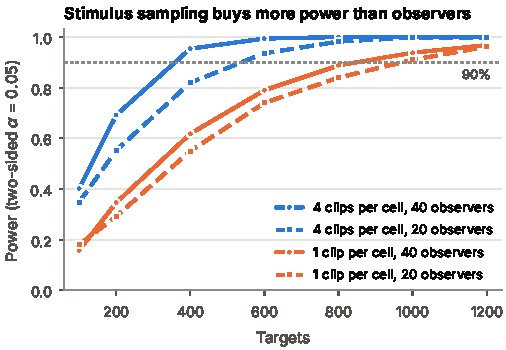
\includegraphics[width=\columnwidth]{figures/figS5_power.pdf}
\caption{\textbf{Simulated power for the Stage-2 information $\times$ ability interaction} (E8; 500 replicates per point).
Assumptions: perceived competence correlates 0.35 with true ability after informative exposure and 0.15 after control
exposure; each clip yields one impression shared by its viewers; choice logit slope 0.8 per SD of perceived competence;
target appeal SD~1; observer intercept SD~0.8; ability measured with reliability 0.8. Analysis: per-target difference in
choice rates regressed on measured ability.}
\label{fig:power}
\end{figure}

\subsection{Stages 3 and 4: field and historical evidence}

Longitudinal and cross-cultural studies in natural-fertility populations should measure $\rho_{ZC}$ (P5) separately for
dominance and prestige (P13), mutual effects (P6), kin decision rules (P7), and the contrast between embodied-capital and
wealth-based economies (P8), testing measurement comparability rather than assuming
it~\cite{vonrueden2016,smith2004,smith2017}. Existing datasets that hold both peer-rated status and cognitive or knowledge
measures, such as the Tsimane studies~\cite{vonrueden2008,vonrueden2011,mcdade2007}, could give a first estimate without new
fieldwork. Historical support requires dated brain-size steps aligned with budget and information innovations (P9), which
the breakpoint intervals of Table~\ref{tab:phases} show to be a weak test at present, and causal evidence that tissue
contributes to capacity (P10). Absence of preserved performance venues is weak evidence, because most performance leaves no
trace.


\section{Limitations and failure regimes}\label{sec:limits}

\noindent The route coefficients ($\beta_N,\beta_D,\beta_S$), the validity $R$, the coupling $a$, the loadings
$\ell_F,\ell_G$, the subordinates' share $q$, and the costs are stipulated, not estimated. The Gaussian, infinitesimal, and
weak-selection assumptions make the propositions exact or tractable; non-Gaussian traits and decentralized matching were
examined only partially, and Gaussian approximations can fail under strong selection~\cite{turelli1994}. Validity is
exogenous in Models I--VII. Model VIII lets a candidate condition delivery on being assessed, the simplest form of
deception, but it does not let observers, tasks and display coevolve, as evolving-assessment models
do~\cite{gavrilets2006,baroudagues2022}; the enforced share is stipulated, not derived from a model of sanction; and the
staging result assumes that capacity is read only at full effort. The bivariate dynamics use Lande's approximation and a fixed $\mathbf G$. The
despot's dilemma is a one-sided optimization with an exogenous price for subordinates; it bounds the skew a dominant would
choose and does not model bargaining, leveling from below, or the arms race in coalition size. The loadings that drive the
aim result are illustrations chosen to show direction, and the net effects quoted for leveling inherit that arbitrariness.

The fossil reanalysis uses published compilations with their taxonomy, dates and volume estimates as given; regional series
are not lineages; and the three datasets overlap without being identical. Breakpoints are estimated with wide intervals, and
stasis cannot be distinguished from slow change within phases. Contemporary correlations (partner correlations,
status--reproduction associations, brain--intelligence correlations) are not ancestral parameters.
Proposition~\ref{prop:identity} separates information from opportunity analytically, but in natural populations the two may
change together, and observational data alone cannot separate them. Bibliographic records were verified against a registry,
but claim-level checks relied mainly on abstracts; a specialist reading of the full texts remains necessary.
The present-day decomposition is phenotypic, from one country, and subject to the limits listed in
Section~\ref{sec:gss}; the drivers of Section~\ref{sec:hidden} are supported by field and survey associations, not by
experiments, and their ancestral importance is conjecture. The generalist results assume independent, equally weighted
domains and a single general factor; correlated specialties and unequal weights change the constants but not the direction.

The speed-dating analysis has four limits. The participants were graduate and professional students at one university,
selected for academic ability, which narrows the range of intelligence and lowers agreement about it, so the number of
observers needed is an upper estimate. A speed date is all test: it says how a first meeting between strangers is judged
and nothing about judgment among people who have known each other for years, which is reached here only through
Eq.~\eqref{eq:sb} and its assumption of independent errors. With five attributes, what observers can read cannot be
separated from what choosers want at a first meeting. And expected interest was recorded on a ten-point scale whose
rescaling is arbitrary; the difference between the sexes does not depend on it, the levels do. The comparative evidence
of Table~\ref{tab:culture} consists of associations across or within societies, several with stated preferences as the
outcome, taken from abstracts; it shows that the weights move with institutions and does not identify why.
Version 9 adds three kinds of evidence, each with its own limit. The ethnographic codes are judgments by outsiders of
societies described in the last two centuries; samples for the most sensitive variables are small and select for societies
in which the matter was recorded; and societies are not independent observations. The cross-national files are convenience
samples answering questionnaires in translation, with unequal numbers by country and more women than men; they are used
for direction and spread, never for rank. The decomposition of falling births is an identity applied to repeated
cross-sections; it locates the change and cannot say why people marry less. The effective-number result is exact for the
model stated and silent on migration, generation length and group-level drift.
Table~\ref{tab:failure} lists the conditions under which the amplification pathway fails.

\begin{table}[t]
\caption{Failure regimes.}\label{tab:failure}
\footnotesize
\begin{tabularx}{\columnwidth}{@{}P{0.40\columnwidth}L@{}}
\toprule
Condition & Consequence\\
\midrule
$R\approx0$ (no target-valid information) & Choice-mediated selection on capacity vanishes (Cor.~\ref{cor:bottleneck})\\
Display dominates score variance & Selection drives presentation, not capacity (Cor.~\ref{cor:score})\\
Standing rests on force ($\bar\ell_G\approx0$) & Selection enlarges bodies, not brains (Prop.~\ref{prop:aim})\\
Preferred cue is a life stage & No heritable response (Cor.~\ref{cor:cue})\\
$\rho_{ZC}\approx0$ & Standing route inert for capacity\\
Equal reproductive output, no standing effect & No directional response despite assortment\\
Contests too dangerous to repeat & Validity stays near $R(1)$ (Prop.~\ref{prop:repeat})\\
Saturating returns only & Budget relaxation yields small tissue gains (Prop.~\ref{prop:persist})\\
$a=0$ & No permanent tissue change; organization absorbs demand (Prop.~\ref{prop:tissue})\\
Budget never relaxes & Demand persists but tissue stays put\\
Access decoupled from performance & Positional demand and tissue investment fall (P8)\\
Validity below Eq.~\eqref{eq:threshold} & Capacity selected, tissue not enlarged (Cor.~\ref{cor:colimit})\\
Gains arise only from inequality & No information effect at fixed opportunity (P12)\\
Each person assessed in one domain & Generalist aim lost; specialties selected (Prop.~\ref{prop:division})\\
Chronology mismatch & Mechanism cannot explain earlier steps\\
\bottomrule
\end{tabularx}
\end{table}

\section{The strongest objections}\label{sec:redteam}

\noindent Each objection is stated in its strongest form before it is answered. Severity is our assessment of the threat to
the hypothesis before the response. Objections marked \emph{accepted} changed the theory or its claims.

\begin{table*}[tp]
\caption{Register of objections, part 1.}\label{tab:red}
\scriptsize
\begin{tabularx}{\textwidth}{@{}P{0.028\textwidth}P{0.225\textwidth}P{0.05\textwidth}LP{0.19\textwidth}@{}}
\toprule
\# & Objection & Severity & Response (where developed) & Residual risk\\
\midrule
O1 & \textbf{The rate is not a puzzle.} Per generation, brain size changed by about $10^{-4}$ SD; any weak force
suffices~\cite{gingerich2022}. & High & Accepted. The explanandum is persistence, cost-paying, parallelism and pattern
(E1--E8), confirmed by reanalysis (Section~\ref{sec:explananda}). & Sufficiency is cheap; discrimination must come from pattern
predictions.\\
O2 & \textbf{Drift fits better.} Neurocranial change in \Homo{} is best fit by random-walk and stasis
models~\cite{hubbe2026}. & High & Magnitude tests reject drift unless $N_e$ was small; cost and three parallel regional series
argue against neutrality; random-walk and stasis signatures are what a constraint-tracking optimum
produces~\cite{estes2007}, and Proposition~\ref{prop:tissue} predicts such steps. & If long-term $N_e\lesssim2{,}000$,
magnitude alone cannot exclude drift.\\
O3 & \textbf{Humans did not choose freely.} Kin arrange most forager marriages~\cite{walker2011}. & Medium & Assessment is
multi-party. Kin observe longer and across more domains; brideservice is a performance-before-outcome institution; parental
preferences select too~\cite{apostolou2007}. & Kin may weigh alliance and wealth over capacity (P7).\\
O4 & \textbf{Games are recent.} All attested formal games are Holocene (Table~\ref{tab:games}); strategy games track political
complexity~\cite{roberts1959}. & Medium & Accepted for games. The mechanism needs public, repeated, outcome-revealing
performance: foraging returns, contests, play, story, song, firelit talk~\cite{wiessner2014,scalise2018}. & Venue antiquity is
inferred, not observed (fire about 1~Ma at one site~\cite{berna2012}).\\
O5 & \textbf{Perceived is not measured intelligence.} Appeal tracks perception~\cite{driebe2021}; displays may signal
condition~\cite{baroudagues2025}. & High & Validity $R$ is explicit. Low $R$ predicts selection on display, not capacity
(Corollary~\ref{cor:score}); portfolios raise $R$ (Propositions~\ref{prop:portfolio}--\ref{prop:diversity}). & If ancestral
$R$ was low, selection fell on presentation.\\
O6 & \textbf{Strategic non-participation and deception.} & Medium & Disclosure unravels when hiding is read as bad
news~\cite{milgrom1981}: threshold hiding by 40\% cuts $R$ only from 0.50 to \HideThr{} (Table~\ref{tab:robust}). Small groups
observe for years. & Coordinated deception (shared presentation bias) is not averaged out.\\
O7 & \textbf{Cognition is selected against today}~\cite{kong2017}. & Medium & Post-transition fertility differs from
natural-fertility settings, where status predicts reproduction~\cite{vonrueden2016}. The identity explains the reversal as a
change of alignment, not of accuracy (Section~\ref{sec:present}). & Ancestral direction for cognition itself is unmeasured.\\
O8 & \textbf{Status is not cognition.} Status--reproduction data say nothing about capacity. & High & Accepted as the key
empirical gap: the standing--capacity correlation $\rho_{ZC}$. Even $\rho_{ZC}=0.05$ gives several times the selection
required (Section~\ref{sec:strength}). & If $\rho_{ZC}\approx0$, the standing route is inert.\\
O9 & \textbf{Mutual choice implies symmetric selection, but the evidence is male-biased.} & Medium & Routes are
sex-specific; the response is the average of the two sexes' differentials. Women's skill is assessed and pays
too~\cite{smith2017,marlowe2004,mcdade2007}. & Female-side field data are thin.\\
O10 & \textbf{Selection on cognition need not enlarge brains.} & High & Proposition~\ref{prop:tissue}: permanent tissue change
requires functional coupling $a>0$; genetic correlation alone is transient. Within-family and experimental evidence supports
coupling~\cite{lee2019,kotrschal2013}; otherwise demand is absorbed by organization~\cite{neubauer2018}. & $a$ is unmeasured
for ancestral populations.\\
O11 & \textbf{Any constant demand would do.} The hypothesis is not discriminating. & High & Rank-based demand is
mean-invariant, while absolute ecological returns saturate (Proposition~\ref{prop:persist}); the information lever $\sqrt{R}$,
the aim, and the decoupling prediction are specific (P2, P8, P13). & Social-competition accounts share
mean-invariance~\cite{flinn2005,crespi2022}.\\
O12 & \textbf{Strong selection would exhaust heritable variance.} & Low & Required selection is weak; assortment inflates
$V_A$ (Proposition~\ref{prop:assort}); cognition has a large mutational target and may capture
condition~\cite{rowe1996,keller2006,millerpenke2007}. & None specific.\\
O13 & \textbf{A Holocene brain decline would contradict the mechanism.} & Low & Timing is contested~\cite{desilva2021,villmoare2022}.
The model predicts relaxation where access decouples from assessed performance, and capacity can be selected without tissue
(Section~\ref{sec:present}). & Sign and timing remain uncertain.\\
O14 & \textbf{Unfalsifiable adaptive story.} & High & \NPred{} predictions with stated weakening results
(Table~\ref{tab:predictions}); powered design (Fig.~\ref{fig:power}). & Historical stages remain weakly testable.\\
O15 & \textbf{Information or inequality?} Apparent accuracy benefits may be more unequal reproduction. & High & Accepted.
Proposition~\ref{prop:identity} separates accuracy from intensity; at fixed opportunity the gain in a pair-output model is $\sqrt2$, not 2
(Table~\ref{tab:identity}). & In nature, information and opportunity may change together.\\
O16 & \textbf{Similar cognition in both sexes is not evidence of mutual choice}~\cite{lande1980}. & Medium & Accepted; Q6
withdrawn as support. Mutual assessment is tested directly (P6). & One supporting argument lost.\\
O17 & \textbf{Copying and runaway yield the same appeal}~\cite{duval2023,lande1981,gouda2018}. & High & These predict appeal
without accuracy; the $2\times2$ information $\times$ endorsement design separates them (Section~\ref{sec:predictions}). & In
nature both operate together.\\
O18 & \textbf{Observation is costly; assessment may not be adopted.} & Medium & Benefit grows as $\sqrt{R(n)}$, concave in
$n$, so per-event costs give an interior optimum (Proposition~\ref{prop:repeat}); one public performance serves many
assessors, and talk spreads the result. & Adoption is not modeled as an evolving strategy.\\
\bottomrule
\end{tabularx}
\end{table*}

\begin{table*}[tp]
\caption{Register of objections, part 2.}\label{tab:rednew}
\scriptsize
\begin{tabularx}{\textwidth}{@{}P{0.028\textwidth}P{0.225\textwidth}P{0.05\textwidth}LP{0.19\textwidth}@{}}
\toprule
\# & Objection & Severity & Response (where developed) & Residual risk\\
\midrule
O19 & \textbf{Comparative data refute sexual selection for brains.} Stronger male competition goes with smaller relative
brains in primates and with no increase across mammals~\cite{schillaci2006,lemaitre2009,fitzpatrick2012}. & High & Accepted as
stated. The hypothesis is not that more sexual selection enlarges brains; it is that accuracy and aim do. Contest-driven
skew aims at the body (Proposition~\ref{prop:aim}). The comparative signal that fits is the association of large brains with
pair-bonded, mutual-assessment systems~\cite{shultz2007,schillaci2006}. & Comparative support is indirect and has other
readings (the cognitive demands of pair bonds).\\
O20 & \textbf{Contests of force select brawn.} Strength is what observers read and what predicts hunting reputation and
mating success~\cite{sell2009,apicella2014,puts2010,hill2013}. & High & Accepted. Physical contest is one venue with a small
loading on capacity; under the illustrative loadings a shift from force to skill and prestige raises selection on capacity
\AimGain-fold at equal intensity (Table~\ref{tab:modelv}). & If ancestral standing rested mainly on force, the standing route
did little for brains.\\
O21 & \textbf{Leveling should slow selection.} Human reproductive skew is low for a mammal~\cite{ross2023}; by the identity,
lower inequality means a smaller response. & High & Accepted. Proposition~\ref{prop:despot} predicts the fall; it lowers
intensity \DesIntLo- to \DesIntHi-fold in the example. Leveling matters because it changes the criterion from force to
conferred standing, not because it intensifies anything. & The net effect on capacity depends on unmeasured loadings.\\
O22 & \textbf{Pleistocene war is unproven.} Most forager killings are personal disputes~\cite{fry2013}; the oldest massacre is
about 10~ka~\cite{lahr2016}. & Medium & Proposition~\ref{prop:despot} needs rival coalitions strong enough to matter, not
chronic war; coalitionary killing by outnumbering is shared with chimpanzees~\cite{wilson2014}. The brain results do not
depend on how often groups fought. & When leveling arose is unknown.\\
O23 & \textbf{Warriors do not reliably out-reproduce others.} Waorani raiders had fewer
descendants~\cite{beckerman2009}. & Medium & Accepted: evidence is mixed~\cite{chagnon1988,glowacki2015}. The model treats
courage as one venue whose payoff depends on local rewards~\cite{glowacki2013}. & The sign of selection on risk-taking is
context-dependent.\\
O24 & \textbf{Fertility and symmetry cues have weak validity and aim at a life
stage}~\cite{lassek2018a,lassek2018b,lassek2019,pound2014}. & Medium & Accepted; these preferences lie outside the mechanism. A cue
dominated by a transient state selects nothing heritable and nothing on capacity (Corollary~\ref{cor:cue}). Female energetics
and obstetrics enter on the budget side. & None for the mechanism.\\
O25 & \textbf{Neanderthals had brains as large as ours in small, inbred
communities}~\cite{prufer2014,skov2022}. & High & Accepted as a constraint. The model does not require large networks:
validity can be high where everyone watches everyone for years. Small communities lower the opportunity for selection and
raise drift, but did not prevent enlargement (Section~\ref{sec:hominins}). & Any version that needs \Hs-scale networks is
contradicted.\\
O26 & \textbf{Small-brained \Homo{} persisted} beside large-brained species~\cite{berger2015,kubo2013}. & Medium & Consistent
with a budget-limited account (islands, small ranges) but also a warning that complex behavior does not require volume,
which bears on the coupling $a$. & The selective regime of those populations is unknown.\\
O27 & \textbf{Brains shrank while status still paid.} Holocene elites had extreme reproductive
success~\cite{karmin2015,zeng2018}, yet volume fell~\cite{ruff1997,desilva2023}. & High & The Holocene raised inequality, not
accuracy, and tied access to inherited wealth and descent group~\cite{borgerhoffmulder2009}: opportunity without alignment.
Body size fell too. Combinations of alleles that today predict measures of cognitive performance rose in West Eurasia over
the same period~\cite{akbari2026}, which Proposition~\ref{prop:tissue} allows when tissue is dear; what those alleles did
in past environments is unknown. & Timing and cause of the decline are unsettled.\\
O28 & \textbf{The brain--intelligence genetic correlation is inflated} by cross-trait assortative
mating~\cite{border2022}. & Medium & The envelope spans $r_g=0.1$--$0.5$ (Table~\ref{tab:envelope}); within-family
associations support a causal contribution of size~\cite{lee2019}. & $r_g$ and $a$ for ancestral populations are unknown.\\
O29 & \textbf{Reputation is too noisy to select on.} Hadza hunting reputations track skill weakly, and hunters cannot be
ranked from short samples~\cite{stibbardhawkes2018,hillkintigh2009}. & High & This is the premise, not a refutation:
single-venue validity is low, and what matters is whether years of observation across venues raise it (P2). Weak validity
still yields weak selection, which is all the rate requires. & If lifetime, multi-venue validity is also near zero, the
mechanism fails.\\
O30 & \textbf{Correlations cannot be multiplied into a selection estimate.} A status--reproduction correlation times a
standing--capacity correlation omits the association of capacity with reproduction at fixed standing, which can have either
sign. & High & Accepted. The comparison in Section~\ref{sec:strength} is now stated as a requirement under an explicit mediation
assumption, with the omitted term written out; no adequacy claim rests on it. & The missing covariance is unmeasured.\\
O31 & \textbf{The tissue model is given its steps.} A model whose costs are lowered at chosen dates reproduces steps by
construction. & High & Accepted. The match in shape is called a consistency check; a test needs independently dated budget
changes (P9). & Dates of fire, cooking and care are too coarse at present.\\
O32 & \textbf{Phenotypic validity is not genetic accuracy.} A score can predict the phenotype better and the breeding value
worse~\cite{hazel1943}. & Medium & Accepted as a remark to Proposition~\ref{prop:identity}; all validity statements concern the
phenotype. & Genetic accuracy of social assessment has never been measured.\\
\bottomrule
\end{tabularx}
\end{table*}

\begin{table*}[tp]
\caption{Register of objections, part 3.}\label{tab:redthree}
\scriptsize
\begin{tabularx}{\textwidth}{@{}P{0.028\textwidth}P{0.225\textwidth}P{0.05\textwidth}LP{0.19\textwidth}@{}}
\toprule
\# & Objection & Severity & Response (where developed) & Residual risk\\
\midrule
O33 & \textbf{The present-day differentials are confounded.} Income is a consequence as well as a cause of family formation;
phenotypic differentials need not be genetic~\cite{morrissey2010,kleven2019}. & High & Four traits are shown, two of them largely
fixed before childbearing; signs agree with polygenic-score studies~\cite{kong2017,hughjones2022}; no causal claim is made
(Section~\ref{sec:gss}). & Causal structure remains unidentified in survey data.\\
O34 & \textbf{``General capacity'' may be opportunity.} A portfolio rewards whatever is common to all venues, including
health, family position and training. & High & Accepted: the general nuisance is selected in the same proportion as general
capacity (Corollary~\ref{cor:generalist}); the claim is about aim relative to specialties, not purity. & If the common factor of
performance is mostly non-heritable, the generalist aim selects little.\\
O35 & \textbf{Foragers do specialize.} Sexual and age division of labor is universal, and individuals favor the tasks they do
best~\cite{hooper2015}. & Medium & Common comparison within sex and age class is what the result needs; partial specialization
weakens the aim by the factor in Proposition~\ref{prop:division}, which is modest for small numbers of domains. & The number of
commonly compared domains has not been measured in any society.\\
O36 & \textbf{Capacity is not commitment.} A capable partner who does not invest is worth little to a chooser, so attraction to
competence need not select competence. & High & Accepted and formalized: selection on capacity through choice is proportional to
mean delivery, and the two traits are complements (Proposition~\ref{prop:delivery}). & Delivery and its validity are unmeasured
in any natural-fertility population.\\
O37 & \textbf{Nothing shows that assessment is more accurate today.} Records are abundant, but so are curation and copied
judgment. & Medium & Accepted. The claim is withdrawn; the text now says that information is abundant and its accuracy relative
to direct observation unmeasured (Section~\ref{sec:present}). & None.\\
O38 & \textbf{A cue that changes with age can still carry heritable variation.} Timing of life-history events is heritable and
selected. & Medium & Accepted. Corollary~\ref{cor:cue} is restricted to the part of a cue that tracks age and state; timing is
treated as a driver in its own right (Section~\ref{sec:hidden}). & The split between state and heritable timing in any cue is
unmeasured.\\
O39 & \textbf{Performance can be faked.} A theory in which assessment drives selection needs an account of honest signaling;
this one took validity as given. & High & Addressed in part. A performance at full effort cannot exceed capacity, so staged
tests are valid for capacity; delivery can be feigned whenever assessment is recognized, and is learned only from unstaged
observation, report or enforcement (Proposition~\ref{prop:staging}); exaggeration in one domain is diluted by breadth
(Corollary~\ref{cor:inflation}). & A general talent for seeming is not diluted by breadth, and the coevolution of display
and scrutiny is not modeled.\\
O40 & \textbf{If sharing is enforced, a wife gains nothing by choosing the producer.} Widely shared meat is a public good, so
enforcement should remove the incentive to choose able partners~\cite{hawkes2002}. & High & Accepted for the bride as sole
assessor. Under enforcement the assessors who matter are those who receive the product and control access: the band that
confers standing and the kin who arrange marriages. Producers' households also keep more than a public-goods account
implies in later Hadza data~\cite{wood2013}. & The enforced share has not been measured as such in any population, and the
model treats enforcement as given.\\
O41 & \textbf{Marriage is not partnership.} Parenthood among the never married says little about whether a gate exists,
because most births outside marriage are to cohabiting couples~\cite{lundberg2016}. & Medium & Accepted. The survey records
marriage, not partnership; the text describes the marriage gate only, and partnerlessness is measured separately
(Fig.~\ref{fig:today}D). & Cohabitation histories are needed to say whether assessment at partnering has weakened.\\
O42 & \textbf{Graduate students in a staged event are not the ancestral camp.} Four minutes with a stranger of similar
schooling says nothing about how intelligence was judged over years among kin. & High & Accepted, and it is the point of
the analysis. The experiment measures the single-observer, single-meeting end of Eq.~\eqref{eq:sb}; the camp is the other
end, reached only by the law. Range restriction lowers agreement about intelligence here, so the observers needed are an
upper estimate (Section~\ref{sec:speed}). & No study has measured agreement about ability among long-acquainted
co-residents with an external criterion for the same people.\\
O43 & \textbf{Legibility and taste are confounded.} Looks may earn the most because they matter most for a first meeting,
not because they are easiest to read. & High & Accepted. Five attributes cannot separate the two, and the correlation of
\SdLegPear{} is reported as a pattern. The theory needs only the weaker statement, which the data support: a trait that
observers cannot agree on cannot carry a consistent selection differential, whatever its value. & Requires the experiment of
prediction P27.\\
O44 & \textbf{Childlessness is not failure of access.} People without children include those who chose none, the infertile
and the late; calling the parenthood episode ``access'' attributes all of it to being chosen. & High &
Accepted. Episodes are named for what the survey records: marrying, becoming a parent, and number of children. Only the
first is a decision by others about the person, and it is labeled the door. Intentions and fecundity are in the second, and
the text says so (Section~\ref{sec:today}). & Fertility intentions and partnership histories for the same respondents would
separate choice from constraint; the survey used has neither in most years.\\
O45 & \textbf{Mate choice assumes consent.} Brides were given, bought and taken; rape and capture were common; so
``choice'' by women cannot have built anything. & High & Accepted as to the word. The mechanism needs an assessor with
years of evidence, and the record names parents and elders (Table~\ref{tab:cultures}). Coercion enters as
Eq.~\eqref{eq:coercion}: it scales the pathway by $1-\kappa$ and selects the body. & $\kappa$ is unknown for every
ancestral population. If it was near one, the pathway did nothing.\\
O46 & \textbf{Ethnographic codes are not data about the Pleistocene.} They are outsiders' judgments of societies
described in the last two centuries, many under colonial pressure. & High & Accepted. The codes are used to show that
free choice by brides is rare in the only record there is, not to estimate ancestral rates. & Coding error is
unquantified; one variable (types of games) was set aside for that reason.\\
O47 & \textbf{The effective-number identity ignores migration, generation time and lineage dynamics.} & Medium &
Accepted, and said in the text. The proposition shows that the headcount cannot be recovered from the ratio; adding these
processes strengthens that conclusion. & None for the claim made.\\
O48 & \textbf{Self-ratings in convenience samples.} The cross-national ``door'' result relates a man's opinion of his
prospects to his having a partner, and having a partner may improve the opinion. & High & Accepted. The result is offered
as agreement in direction with the register-like survey result for the United States, in 35 of 50 countries, and nothing
more. & Needs income records and partnership histories in several countries.\\
O49 & \textbf{Falling births have many causes.} Housing, wages, contraception, women's schooling and changing wishes all
matter; blaming the loss of community is a fashion. & High & Partly accepted. The decomposition is an accounting. It shows
where the births are missing, at union formation, and that stated ideals did not fall. Three findings against the simple
community story are reported in the same section. & The mechanism of Proposition~\ref{prop:waiting} is untested (P34,
P35).\\
O50 & \textbf{Projecting diagnoses onto the past.} Speaking of attention deficit or neurodivergence in foragers treats
modern clinical categories as natural kinds. & Medium & Accepted. The text speaks of trait variation and of one gene, gives
the evidence against as well as for, and claims only Corollary~\ref{cor:narrow}. & The corollary is untested in people
(P33).\\
O51 & \textbf{One case is an anecdote.} The Maasai tournament is a conservation program reported by its organizers and
the press. & Medium & Accepted. It is used as an illustration of Corollary~\ref{cor:ritual}, with two peer-reviewed
studies of lion killing and one of ritual fights and reproduction. & No data yet on what tournament rank predicts
(P32).\\
\bottomrule
\end{tabularx}
\end{table*}

\section{How old are games?}\label{sec:games}

\noindent Table~\ref{tab:games} lists the oldest known games. The list shows why formal games cannot be the cause. The oldest secure board games are about 5,000 years old, the oldest depictions of wrestling and
boxing a little younger, and the oldest candidate game boards under 8,000 years. Brains had reached their modern size by
300,000 to 100,000 years ago (Section~\ref{sec:explananda}). Formal games are therefore evidence of a human propensity to stage
public, rule-bound, repeatable contests, and of what institutions do with that propensity; they are not candidates for the
cause. The ancestral analogue has to be sought in what leaves no boards: play, wrestling, races, target contests, song and
verbal dueling, which are documented across the ethnographic record~\cite{roberts1959,deaner2013,scalise2018}, and which have
precursors in the play fighting that adult primates use to assess and manage one another~\cite{pellis2000}.

\begin{table}[t]
\caption{Oldest attested formal games and contests. Dates are for the earliest secure evidence.}\label{tab:games}
\scriptsize
\begin{tabularx}{\columnwidth}{@{}P{0.30\columnwidth}LP{0.13\columnwidth}@{}}
\toprule
Game or contest & Earliest evidence and place & Source\\
\midrule
Rows of pits cut in stone slabs (possible boards) & c.~5800~BCE, `Ain Ghazal, Jordan; function disputed & \cite{rollefson1992}\\
Senet and mehen & c.~3100--2700~BCE, Egypt: First Dynasty boards, Third Dynasty tomb painting & \cite{crist2016}\\
Twenty squares (``Royal Game of Ur'') & c.~2600~BCE, Ur; rules on a cuneiform tablet of 177~BCE & \cite{devoogt2013,finkel2007}\\
Fifty-eight holes (``hounds and jackals'') & Late third to early second millennium~BCE; southwest Asia, Egypt, Caspian shore &
\cite{devoogt2013,crist2025}\\
Wrestling, boxing, stick fighting & Third-millennium~BCE Mesopotamian plaques and figurines; hundreds of wrestling pairs
painted at Beni Hasan, Egypt, c.~2000~BCE & \cite{poliakoff1987,decker1992}\\
Rubber-ball game & Rubber balls c.~1600~BCE; ball court c.~1650~BCE; highland court 1374~BCE; Mesoamerica &
\cite{hosler1999,hillclark2001,blomster2020}\\
Dice and gambling games & Widespread across North America at contact, with older gaming pieces & \cite{deboer2001}\\
\bottomrule
\end{tabularx}
\end{table}

\section{Additional tables for the present-day analysis}\label{sec:sitables}

\begin{table*}[!ht]
\caption{Access--number decomposition by birth cohort (General Social Survey, ages 45--79). Units and intervals as in
Table~\ref{tab:gss}. Cells with fewer than 300 respondents are omitted.}\label{tab:gsscohort}
\scriptsize
\begin{tabularx}{\textwidth}{@{}P{0.15\textwidth}llrCCC@{}}
\toprule
\tabinput{generated/tab_gss_cohort.tex}
\bottomrule
\end{tabularx}
\end{table*}

\begin{table*}[!ht]
\caption{Robustness of the decomposition for schooling and income. Intervals are from 400 bootstrap resamples.}\label{tab:gssrobust}
\scriptsize
\begin{tabularx}{\textwidth}{@{}P{0.17\textwidth}P{0.16\textwidth}CCC@{}}
\toprule
\tabinput{generated/tab_gss_robust.tex}
\bottomrule
\end{tabularx}
\end{table*}

\begin{table*}[!ht]
\caption{Three episodes of selection (General Social Survey, ages 45--79, cohorts 1900--1979): pairing is the mean standardized
trait among the ever-married; conversion is the further difference between parents and the ever-married; number is as in
Table~\ref{tab:gss}. The three sum to the total. Units: standard deviations of the trait per generation; 95\% bootstrap
intervals from 1,000 resamples.}\label{tab:gssthree}
\scriptsize
\begin{tabularx}{\textwidth}{@{}P{0.17\textwidth}lCCCC@{}}
\toprule
\tabinput{generated/tab_gss_three.tex}
\bottomrule
\end{tabularx}
\end{table*}

\begin{table*}[!ht]
\caption{The pairing gate by birth cohort (General Social Survey, ages 45--79). Never married: percentage who had never
married when interviewed. Parents among the never married: percentage of those with at least one child. Children of the
never married: their share of all children reported by respondents of that sex and cohort. Pairing differential: mean
standardized log income among the ever-married (the first term of Table~\ref{tab:gssthree}), income measured at ages
45--64. 95\% bootstrap intervals from 1,000 resamples in brackets.}\label{tab:gssgate}
\scriptsize
\begin{tabularx}{\textwidth}{@{}llCCCC@{}}
\toprule
\tabinput{generated/tab_gss_gate.tex}
\bottomrule
\end{tabularx}
\end{table*}

\begin{table*}[!ht]
\caption{Said and did in the Columbia speed-dating experiment~\cite{fisman2006}. Said: mean points of 100 given to each
attribute before the event. Did: change in the probability of a yes, in percentage points, per standard deviation of the
rating, with a fixed effect for each chooser, using the chooser's own rating or the mean rating the partner received from
everyone else (panel). Agreement: intraclass correlation between two observers of the same person; observers for 0.8 follows
Eq.~\eqref{eq:sb}. W: women choosing; M: men choosing. Shared interests belong to a pair, so no agreement is defined.}\label{tab:speed}
\scriptsize
\begin{tabularx}{\textwidth}{@{}Lrrrrrrrr@{}}
\toprule
\tabinput{generated/tab_speed.tex}
\bottomrule
\end{tabularx}
\end{table*}

\begin{table*}[!ht]
\caption{Family size by marital history (General Social Survey, ages 45--79, cohorts 1900--1979). Relative family size is
the number of children divided by the mean for the respondent's sex and decade of birth; 95\% bootstrap intervals from 500
resamples in brackets.}\label{tab:gsshist}
\scriptsize
\begin{tabularx}{\textwidth}{@{}lLrrrC@{}}
\toprule
\tabinput{generated/tab_gss_hist.tex}
\bottomrule
\end{tabularx}
\end{table*}

\begin{table*}[!ht]
\caption{Spouses' schooling compared, by birth cohort of the respondent (General Social Survey, currently married
respondents aged 25 and over). 95\% bootstrap intervals from 500 resamples in brackets.}\label{tab:gsshyp}
\scriptsize
\begin{tabularx}{\textwidth}{@{}lrCCCr@{}}
\toprule
\tabinput{generated/tab_gss_hyp.tex}
\bottomrule
\end{tabularx}
\end{table*}

\section{Proofs}\label{app:proofs}

\noindent\textbf{Gaussian tilting lemma.} Let $(A,\mathbf X)$ be jointly Gaussian and $w=\exp(\mathbf h^\top\mathbf X)$. Then
$\E[Aw]/\E[w]=\E[A]+\Cov(A,\mathbf h^\top\mathbf X)$, by differentiating the joint moment-generating function. If instead
$w=\exp(kx-\tfrac c2x^2)$ with $x\sim\N(0,V)$, the tilted law of $x$ is $\N\big(kV/(1+cV),\,V/(1+cV)\big)$.

\textbf{Proposition~\ref{prop:identity}.} Write $\E[A\mid Y]=\mu+\kappa(Y-\E Y)$ with $\kappa=\Cov(A,Y)/V_Y$. The residual
$A-\E[A\mid Y]$ is uncorrelated with every function of $Y$, so
$\Cov(A,W)=\Cov(\E[A\mid Y],W)=\kappa\,\SD(Y)\Corr(Y,W)\SD(W)$, and $\kappa\,\SD(Y)=\sigma_A\Corr(A,Y)$. Under
Eq.~\eqref{eq:score}, $\Corr(A,Y)=\lambda V_A/(\sigma_A\SD(Y))=h\sqrt R$. Dividing by $\E W$ gives Eq.~\eqref{eq:identity}.
Without linearity the first equality still holds and Cauchy--Schwarz gives the bound. If $W$ depends on $Y$ only through
$Z$, the distribution of $W$ and $\Corr(Y,W)=\Corr(Z,W)$ do not depend on $R$. \qed

\textbf{Proposition~\ref{prop:routes}.} In the infinite-population limit with equal marginal score distributions, ideal rank
matching pairs equal scores, so the partner's score is $Y_p=Y$ and $Z_p=Z$. Then $C_p=\E[C_p\mid Y]+\varepsilon$ with
$\E[C_p\mid Y]=\mu+(\lambda V_P/V_Y)(Y-\E Y)$ and $\varepsilon$ independent of everything about the focal individual, so
$(A,C,C_p,Z)$ is jointly Gaussian. The lemma gives $S=\Cov(A,\beta_NC+\beta_DC_p+\beta_SZ)$. Here $\Cov(A,C)=V_A$;
$\Cov(A,Z)=\lambda V_A/\SD(Y)=V_A\sqrt{R/V_P}$ because $\sqrt R=\lambda\sqrt{V_P}/\SD(Y)$; and
$\Cov(A,C_p)=(\lambda V_P/V_Y)\lambda V_A=V_AR$. Each offspring has one parent of each sex, so
$\Delta\bar A=\tfrac12(S_f+S_m)$ under unbiased transmission. With unequal score marginals, rank matching equates quantiles
and the same argument applies to standardized scores. \qed

\textbf{Corollaries~\ref{cor:bottleneck}--\ref{cor:score}.} Corollary~\ref{cor:bottleneck} sets $R=0$.
A pair-output model $W=\exp[b(C_f+C_m)/2]$ implies $\beta_N=\beta_D=b/2$ and $\beta_S=0$ for each parent. For
Corollary~\ref{cor:score}, $\Cov(A_D,Z)=V_{A,D}/\SD(Y)$ and $\Cov(A,Z)=\lambda V_A/\SD(Y)$. \qed

\textbf{Propositions~\ref{prop:portfolio} and~\ref{prop:diversity}.} The domain average of $G$ is $G$; the average of $K$
independent domain terms has variance $(V_S+\tau^2+\sigma^2[\rho+(1-\rho)/n])/K$; $\Omega$ adds $\omega^2$. So $V_Y$ is the
denominator of Eq.~\eqref{eq:RG} and $\Cov(G,Y)=V_G$, giving $R_G=V_G^2/(V_GV_Y)$. For Proposition~\ref{prop:diversity}, write
each breeding value as $A_X=h_X^2X+\eta_X$ with $\eta_X$ independent of the score; then
$\Cov(A_G,Z)=h_G^2V_G/\SD(Y)$, $\Cov(A_{S_k},Z)=h_S^2V_S/(K\,\SD(Y))$, and $\Cov(A_\Omega,Z)=h_\Omega^2\omega^2/\SD(Y)$, and
the lemma applies. \qed

\textbf{Proposition~\ref{prop:assort}.} An offspring's breeding value is $(A_f+A_m)/2+\delta$ with $\Var(\delta)=V_{LE}/2$ in
the infinitesimal model~\cite{bulmer1980}. Because pairing depends on $A$ only through $C$ and $\E[A\mid C]=h^2C$,
$\Cov(A_f,A_m)=h^4\Cov(C_f,C_m)=mh^2V_A$. Log-linear selection on jointly Gaussian pairs shifts means without changing
covariances (lemma), giving Eq.~\eqref{eq:assort}. Setting $V_{A,t+1}=V_{A,t}=V$ and $h^2=V/(V+V_E)$ yields
$(1-m)V^2+(V_E-V_{LE})V-V_{LE}V_E=0$, whose product of roots is negative for $m<1$, so exactly one root is positive. For
$m=1$ the equation is linear with root $V_{LE}V_E/(V_E-V_{LE})$, positive only if $V_E>V_{LE}$; otherwise variance grows
without bound. The response follows from $\Cov(A,X)=\tfrac12V_A(1+m)$. \qed

\textbf{Proposition~\ref{prop:persist}.} Write $C=\mu+x$ and $Y-\E Y=\lambda x+\nu$ with $\nu$ independent of $x$ and $A$.
Then $\ln w=(\beta_N-c\mu+\beta_S\lambda/\SD(Y))x-\tfrac c2x^2+(\beta_S/\SD(Y))\nu+\text{const}$. The $\nu$ term tilts only
$\nu$. By the lemma the tilted mean of $x$ is $kV_P/(1+cV_P)$ with $k=\beta_N+\beta_S\sqrt{R/V_P}-c\mu$, and
$\E[A-\mu\mid x]=h^2x$, so $\Delta\bar A=V_Ak/(1+cV_P)$. Setting $k=0$ gives $\mu^*$. For the saturating benefit,
$\E[f'(C)]=\beta_Ee^{V_P/2\kappa^2-\mu/\kappa}$; differentiating $\ln\E[f'(C)]=\ln(c\mu)$ with respect to $\ln(1/c)$ gives
elasticity $\kappa/(\kappa+\mu^*)$. Corollary~\ref{cor:surplus}: $\E[Z]=0$, so $\E[\ln w]=\beta_N\mu-\tfrac c2(\mu^2+V_P)$,
maximized at $\mu=\beta_N/c$. \qed

\textbf{Proposition~\ref{prop:tissue}.} With $\ln w=\beta_{\mathrm{eff}}(aB+K)-\tfrac{\kappa_B}2B^2-\tfrac{\kappa_K}2K^2$ plus
terms independent of the means, the selection gradient at the means is
$\bm\beta=(a\beta_{\mathrm{eff}}-\kappa_B\bar B,\ \beta_{\mathrm{eff}}-\kappa_K\bar K)$ to first order. Lande's equation has a
stationary point only where $\mathbf G\bm\beta=\mathbf 0$, which for nonsingular $\mathbf G$ requires $\bm\beta=\mathbf 0$,
giving Eq.~\eqref{eq:tissue}. With $a=0$ the tissue component of $\bm\beta$ is $-\kappa_B\bar B$, so $\bar B\to0$ regardless
of the off-diagonal elements of $\mathbf G$. With positive-definite $\mathbf G$ and $\kappa_B,\kappa_K>0$ the eigenvalues of
$\mathbf G\,\mathrm{diag}(\kappa_B,\kappa_K)$ are positive, so the equilibrium is stable whenever they are below two, which
holds under weak selection. Corollary~\ref{cor:colimit}: the tissue component of $\bm\beta$ is positive exactly when
Eq.~\eqref{eq:threshold} holds; substituting the maximal validity of Proposition~\ref{prop:portfolio} into $B^*$ gives
$B_{\max}$. \qed

\textbf{Proposition~\ref{prop:aim} and Corollary~\ref{cor:cue}.} $(A_F,A_G,Y)$ is jointly Gaussian, so $\E[A_X\mid Y]$ is
linear and the first line of the proof of Proposition~\ref{prop:identity} gives
$S_{A_X}=[\Cov(A_X,Y)/\SD(Y)]\,\Corr(Y,W)\CV(W)$ for $X\in\{F,G\}$. Writing $A_X=h_X^2X+\eta_X$ with $\eta_X$ independent of
$Y$, $\Cov(A_F,Y)=h_F^2\bar\ell_FV_F$ and $\Cov(A_G,Y)=h_G^2\bar\ell_GV_G$. The ratio is free of $i$ and of
$\SD(Y)$. For the corollary, $\Cov(A_Q,Q)=V_{A_Q}$ and $\Cov(A_G,Q)=0$. \qed

\textbf{Proposition~\ref{prop:repeat}.} Put $\alpha=\lambda^2V_P$, $b_0=\tau^2+\rho\sigma^2$ and $c_0=(1-\rho)\sigma^2$, so
$R(n)=\alpha/(\alpha+b_0+c_0/n)$. Then
$g(n)\equiv\mathrm d\sqrt{R}/\mathrm dn=\tfrac12\sqrt{R}\,c_0/\big(n[(\alpha+b_0)n+c_0]\big)>0$ and
\[
\frac{\mathrm d\ln g}{\mathrm dn}=-\frac{4(\alpha+b_0)n+c_0}{2n[(\alpha+b_0)n+c_0]}<0 ,
\]
so $g$ is strictly decreasing, with $g\to\infty$ as $n\to0$ and $g\to0$ as $n\to\infty$. The first-order condition
$g(n^*)=\delta/B$ therefore has exactly one root, which decreases as $\delta/B$ rises; when the root is below one, a single
event or none is optimal. $R$ is increasing in $n$, so $R(n^*)$ falls as $\delta/B$ rises. The fixed-risk form substitutes
$n=D/\delta$. \qed

\textbf{Proposition~\ref{prop:despot}.} For $0\le k<1/q$,
\[
\phi(k)\equiv\frac{\mathrm d\ln U}{\mathrm dk}=-\frac{q}{1-kq}+\frac{\theta\,[1-p(k)]}{1+k}.
\]
The first term is strictly decreasing in $k$; so is the second, because $p$ is increasing in $k$. Hence $\ln U$ is strictly
concave with a unique maximizer, and $k^*>0$ exactly when $\phi(0)>0$, that is when $\theta M^\theta/(1+M^\theta)>q$. For
every $k$, $1-p(k)$ is increasing in $M$ and $-q/(1-kq)$ is decreasing in $q$, so $\phi$ shifts up with $M$ and down with $q$
and its root moves accordingly. As $M\to\infty$, $1-p\to1$ and $\phi(k)\to-q/(1-kq)+\theta/(1+k)$, whose root is
$k=(\theta-q)/[q(1+\theta)]$, leaving the dominant the share $1-kq=(1+q)/(1+\theta)$. \qed

\textbf{Corollary~\ref{cor:generalist} and Proposition~\ref{prop:time}.} Divide the first expression in
Eq.~\eqref{eq:diversity} by the second. For Proposition~\ref{prop:time}, set Eq.~\eqref{eq:RG} equal to $R^*$:
$D=Q/K+(1-\rho)\sigma^2/(Kn)$, and solve for $n$; the right side exceeds the left for every $n$ when $KD\le Q$. \qed

\textbf{Proposition~\ref{prop:polymath}.} The score is $Y=K^{-1}\sum_k(T_k+U_k+\bar e_k)+\Omega$, so $\partial Y/\partial g=1$ and
$\partial Y/\partial s_k=1/K$. With $\ln w=\beta_S(Y-\E Y)/\SD(Y)-\tfrac12c_Gg^2-\tfrac12c_S\sum_ks_k^2$ the gradients of log
fitness are $\beta_S/\SD(Y)-c_Gg$ and $\beta_S/(K\,\SD(Y))-c_Ss_k$, linear in the traits, so under Lande's equation the means
are stationary where they vanish, which gives Eq.~\eqref{eq:gstar}. The costs at equilibrium are
$\tfrac12c_Gg^{*2}=\beta_S^2/(2c_G\SD(Y)^2)$ and $K\cdot\tfrac12c_Ss_k^{*2}=\beta_S^2/(2Kc_S\SD(Y)^2)$; their ratio is $Kc_S/c_G$,
which gives Eq.~\eqref{eq:share}. \qed

\textbf{Proposition~\ref{prop:division} and the remark following it.} Let $k^*=\arg\max_kS_k$. $G$ is independent of the
choice, so $\Cov(A_G,Y\mid k^*)=h_G^2V_G$. Given $k^*=k$, $S_k$ is distributed as the largest of $K$ independent $\N(0,V_S)$
variables, with variance $c_KV_S$. Before selection $A_{S_k}=h_S^2S_k+\epsilon$ with $\epsilon$ independent of all the $S_j$
and hence of the choice, so $\Cov(A_{S_k},Y\mid k^*=k)=h_S^2c_KV_S$. The ratio is Eq.~\eqref{eq:division}; dividing
Eq.~\eqref{eq:aimK} by it gives $Kc_K$. The statement concerns covariances, which determine the selection differential
exactly under linear fitness and to first order in $\beta_S$ under exponential fitness, since the maximum of normal
variables is not normal. For the remark, Stein's lemma gives $\Cov(X_i,f(\mathbf X))=\sum_j\Cov(X_i,X_j)\E[\partial
f/\partial X_j]$ for jointly normal $\mathbf X$; with $f=\max_k(G+S_k+U_k+\bar e_k)$, $\partial f/\partial G=1$ and
$\partial f/\partial S_k=\mathbf 1\{k=\arg\max\}$, which has expectation $1/K$. \qed

\textbf{Proposition~\ref{prop:episodes} and Corollary~\ref{cor:floor}.} With $\E z=0$ and $\bar c_+=\E[c\mid c>0]$,
$\Cov(z,w)=\E[zc]/(p\bar c_+)=\E[zc\mid c>0]/\bar c_+=\E[z\mid c>0]+\Cov(z,c\mid c>0)/\bar c_+$. Also
$\E w^2=\E[c^2\mid c>0]/(p\bar c_+^2)=(1+I_{c>0})/p$, so $I=(1+I_{c>0})/p-1$. For the corollary, the standardized score $Z$ of
those retained has mean $\varphi(z_q)/(1-q)$, and $\E[A\mid Z]=\sigma_Ah\sqrt R\,Z$ under the assumptions of
Proposition~\ref{prop:identity}; $w$ takes the values 0 and $1/(1-q)$, so $\Var(w)=q/(1-q)$. \qed

\textbf{Proposition~\ref{prop:delivery}.} Let $\hat b=\bar b+\kappa_b(Y_b-\E Y_b)$ and $\hat p=\bar p+\kappa_p(Y_p-\E Y_p)$ be the
posterior means from independent signals, so that $\hat v=\hat p\hat b+\hat c-\hat h$ with the last two terms independent of
$A_B$ and $A_P$. Then $\Cov(A_B,\hat p\hat b)=\bar p\,\Cov(A_B,\hat b)+\E[A_B(\hat p-\bar p)(\hat b-\bar b)]$; the last term
vanishes by independence, and $\Cov(A_B,\hat b)=\kappa_b\lambda_bV_{A,B}=R_bV_{A,B}$ as in Proposition~\ref{prop:routes}. The
same argument gives $S_{A_P}$. Under Lande's equation the means change by $V_{A,B}(sR_b\bar p-c_B\bar b)$ and
$V_{A,P}(sR_p\bar b-c_P\bar p)$, a linear system whose matrix has a positive eigenvalue exactly when
$s^2R_bR_p>c_Bc_P$. With $\bar p$ held at one the first equation has the stationary point $\bar b^*=sR_b/c_B$. \qed

\textbf{Proposition~\ref{prop:staging}.} (i)~The mean of $dn$ staged performances is $b$ plus an error of variance
$\sigma^2/(dn)$, which gives $R_b$. Let $m=(1-d)n$. The number of defaults is $F\mid q\sim\mathrm{Binomial}(m,q)$, so
$\Cov(F,q)=mV_P$ and, by the law of total variance, $\Var F=m^2V_P+m\,\E[q(1-q)]$. Hence
$\Corr^2(F,q)=mV_P/(mV_P+\nu)$, which is $R_p$; no assumption about the distribution of $q$ is needed. (ii)~The first
statement is the binomial probability of no default in $m$ trials; setting it to one half and to 0.05 gives the other two.
(iii)~With $A$ and $C$ as defined, $1/(R_bR_p)=(1+A/d)(1+C/(1-d))$. Setting the derivative to zero gives
$A(1-d)(1-d+C)=Cd(d+A)$, that is $(A-C)d^2-2A(1+C)d+A(1+C)=0$. Writing $u^2=A(1+C)$ and $v^2=C(1+A)$, so that
$u^2-v^2=A-C$, the root in $(0,1)$ is $d^*=(u^2-uv)/(u^2-v^2)=u/(u+v)$. The product is zero at both ends and positive
between, so the stationary point is the maximum. \qed

\textbf{Proposition~\ref{prop:enforce}.} (i)~Replace $\hat p$ by $e+(1-e)\hat p$ in the proof of
Proposition~\ref{prop:delivery}: $\Cov(A_B,[e+(1-e)\hat p]\hat b)=[e+(1-e)\bar p]R_bV_{A,B}$ and
$\Cov(A_P,[e+(1-e)\hat p]\hat b)=(1-e)\bar bR_pV_{A,P}$. (ii)~Under Lande's equation the means change by
$V_{A,B}(sR_b[e+(1-e)\bar p]-c_B\bar b)$ and $V_{A,P}(sR_p(1-e)\bar b-c_P\bar p)$. At the origin the first is $V_{A,B}sR_be>0$.
Setting both to zero gives $\bar p=T(1-e)[e+(1-e)\bar p]$, hence Eq.~\eqref{eq:enforceeq}. The Jacobian has negative trace
and determinant proportional to $c_Bc_P-s^2R_bR_p(1-e)^2$, positive when $T(1-e)^2<1$. The interior solution satisfies
$\bar p^*\le1$ exactly when $T(1-e)\le1$, which implies $T(1-e)^2<1$; otherwise $\bar p$ rises to its bound, where the
delivered share is one. (iii)~The delivered share at equilibrium is $\delta^*=e/(1-T(1-e)^2)$, with derivative proportional
to $1-T(1-e^2)>0$. Writing $x=1-e$, $\bar p^*=Tx(1-x)/(1-Tx^2)$ has derivative proportional to $1-2x+Tx^2$, whose only root
in $(0,1)$ is $x=(1-\sqrt{1-T})/T$. \qed

\textbf{Corollary~\ref{cor:inflation}.} Exaggeration $f_k$ enters the score exactly as $s_k$ does in the proof of
Proposition~\ref{prop:polymath}, with $\partial Y/\partial f_k=1/K$ and cost $\tfrac12c_Ff_k^2$, so the gradient of log
fitness is $\beta_S/(K\,\SD(Y))-c_Ff_k$ and the total cost at equilibrium is $\beta_S^2/(2Kc_F\SD(Y)^2)$. Heritable variation
in $f_k$ is a domain-specific trait and Eq.~\eqref{eq:aimK} applies to it. \qed

\textbf{Equation~\eqref{eq:coercion}.} Relative fitness is $w=(1-F)w_a+Fw_f$, where $F$ indicates a coerced mating,
independent of $A$ with mean $\kappa$, and $w_a$, $w_f$ are relative fitness under assessment and under force. Then
$\Cov(A,w)=(1-\kappa)\Cov(A,w_a)+\kappa\Cov(A,w_f)$. \qed

\textbf{Proposition~\ref{prop:ancestors}.} For a sex with offspring number $k$, the variance effective number in a large
population is $N\bar k/(\bar k-1+V/\bar k)$~\cite{kimura1963}. With a share $q$ at zero and the rest at mean
$m=\bar k/(1-q)$ and variance $m+\alpha m^2$, $\E[k^2]=(1-q)\big(m+(1+\alpha)m^2\big)=\bar k+(1+\alpha)\bar k^2/(1-q)$, so
$V/\bar k=1+\bar k\big[(1+\alpha)/(1-q)-1\big]$ and $\bar k-1+V/\bar k=\bar k(1+\alpha)/(1-q)$. For a marker inherited
through one sex, the relevant count is offspring of that sex. If each offspring is of that sex with probability
one-half, the count has mean $\bar k/2$ and variance $V/4+\bar k/4$, and substituting gives the same ratio. \qed

\textbf{Proposition~\ref{prop:waiting}.} By Proposition~\ref{prop:staging} only unstaged occasions inform about delivery,
so after $t$ periods there are $n=k\lambda(1-d)t$ independent observations, with reliability $nr_1/(1+(n-1)r_1)$
(Eq.~\ref{eq:sb}). Setting this to $R^*$ and solving, $n=R^*(1-r_1)/[r_1(1-R^*)]$. \qed

\textbf{Corollary~\ref{cor:ritual}.} Solve $n\rho_s/(1+(n-1)\rho_s)\ge\rho_d$ for $n$. The second statement is
Proposition~\ref{prop:staging} with $d=1$. \qed

\textbf{Corollary~\ref{cor:narrow}.} The assessed score is $Y_T=G+x\,\bar a_T+\bar\varepsilon_T$ with $x$ independent of
$G$, so $\Cov(Y_T,x)=\bar a_T\Var(x)$ and $\Cov(Y_T,G)=\Var(G)$ for every $T$; the gradients follow from
Proposition~\ref{prop:identity}. \qed

\section{Reproducibility and data}\label{app:repro}

\noindent The accompanying package contains the \LaTeX{} source, the bibliography, all scripts, machine-readable results,
and figures. \texttt{code/run\_all.sh} executes, in order, the experiments (\texttt{exp\_core.py}, \texttt{exp\_rates.py},
\texttt{exp\_power.py}, \texttt{exp\_contest.py}, \texttt{exp\_polymath.py}, \texttt{exp\_verify.py}, \texttt{exp\_speed.py},
\texttt{exp\_gss.py}, \texttt{exp\_village.py}, \texttt{exp\_cultures.py}, \texttt{exp\_world.py}, \texttt{exp\_notes.py}), the audit
(\texttt{audit.py}), the figures (\texttt{make\_figures.py}) and the manuscript inputs (\texttt{make\_tex.py}); total runtime
on one CPU core is about twenty minutes, most of it the evolutionary simulations and the bootstraps. Each script writes JSON
outputs to \texttt{results/} with its seed, sizes, parameters, and verification statistics. Figures are generated only from
those files and from the datasets. Every analysis-derived number in the text and every generated table is written
by \texttt{make\_tex.py} into \texttt{paper/generated/}, so the manuscript cannot drift from the results. The bibliography
is produced by \texttt{build\_bib.py} from Crossref records; the verification log is \texttt{results/ref\_verification.json}.
Of \RefCited{} references cited, \RefResolved{} have a DOI that was resolved against Crossref; abstracts could be retrieved
for most of them and specific claims were checked against those abstracts. Where no abstract was available the citation is
limited to what the title states. The manuscript compiles with \texttt{pdflatex}, \texttt{bibtex}, and two further
\texttt{pdflatex} passes.

\emph{Third-party data.} The fossil reanalysis uses three open datasets, redistributed in \texttt{data/} with attribution
and unmodified: Supplementary Dataset~1 of Gingerich~\cite{gingerich2022} (233 specimens; CC~BY~4.0); Supplementary File~2 of
Will et al.~\cite{will2021} (166 \Homo{} specimens with taxon, age and site coordinates; CC~BY~4.0); and the dataset of Du et
al.~\cite{du2018} (94 specimens; Dryad \texttt{doi:10.5061/dryad.c30g9}; CC0). Regional assignment of Middle Pleistocene
specimens uses site coordinates and is coded in \texttt{load\_fossils.py}. The present-day analysis uses the public
cumulative file of the General Social Survey, 1972--2024~\cite{gss2024}, as packaged for R by Healy~\cite{healygssr}. The file
is not redistributed: \texttt{code/fetch\_gss.py} downloads it and extracts the variables used, and \texttt{rda\_reader.py}
reads it without R. The speed-dating analysis uses the public file of the Columbia experiment~\cite{fisman2006}; it too is
not redistributed, and \texttt{code/fetch\_speed.py} copies it from a public mirror and checks its SHA-256 digest. Both
analyses use respondent-level public data with no identifiers, report only aggregates by sex and cohort, and make no
comparison among racial, ethnic or national groups. Three further sources are fetched by scripts and not redistributed:
the D-PLACE release of the ethnographic codes (\texttt{fetch\_dplace.py}, pinned to a commit), and the 175-country and
45-country survey files (\texttt{fetch\_open.py}, checked by SHA-256 digest; the first is licensed CC~BY~4.0). In those
analyses countries and societies are units of replication; none is named or ranked, and variables describing religion or
ethnicity are not read. No new data were collected from human
participants; all simulation data are synthetic.


{\footnotesize\setlength{\bibsep}{0.5pt plus 0.4pt}
\bibliographystyle{unsrtnat}
\bibliography{refs}}

\newcommand{\authorphoto}[2]{\IfFileExists{#1}{\includegraphics[width=0.92in,height=1.17in,keepaspectratio]{#1}}%
{\colorbox{band}{\parbox[c][1.17in][c]{0.92in}{\centering\sffamily\bfseries\LARGE\color{ink2}#2}}}}
\newcommand{\authorbio}[3]{\par\vspace{9pt}\noindent\begin{minipage}[t]{0.98in}\vspace{0pt}#1\end{minipage}\hfill
\begin{minipage}[t]{\dimexpr\columnwidth-1.10in}\vspace{0pt}\small\RaggedRight{\sffamily\bfseries #2}\; #3\end{minipage}\par}
\section*{About the authors}
\authorbio{\authorphoto{figures/author_taylor.jpg}{JT}}{Jepson Taylor}{is chief executive and chief technology officer of
VEOX Inc., which builds AI systems that generate algorithms and optimizers on demand. He was chief AI strategist at
DataRobot and at Dataiku, co-founded Zeff.ai, a deep-learning company acquired by DataRobot in 2020, and earlier led data
science at HireVue, where his work contributed to fourteen patents. He began in semiconductor manufacturing at Intel and
Micron and in quantitative finance. He teaches an executive course on AI at New York University and is the author of
\emph{The Last Commit}.}
\authorbio{\authorphoto{figures/author_beilharz.png}{EB}}{Erin Beilharz}{is a principal consultant at Lufthansa Systems
and an advisor to Navon, which develops modular green data centres for the Global South. She works on AI, clean
technology and digital infrastructure, and speaks on data sovereignty, energy pragmatism and the ethical dilemmas of an
automated world.}
\par\vspace{6pt}\noindent{\sffamily\scriptsize\color{ink2} Biographical details are taken from the authors' public speaker
pages (November 2026) and are to be confirmed by the authors.\par}
\end{document}
